\documentclass[a4paper,11pt]{jsreport}

\usepackage{comment}
\usepackage{float}
\usepackage{color}
\usepackage{multicol}
\usepackage[dvipdfmx]{graphicx}
\usepackage{wrapfig}
\usepackage{graphicx} 
\usepackage{tikz}
\usepackage{enumerate}
\usepackage{bm}
\usepackage{url}
\usepackage{underscore}
\usepackage{colortbl}
\usepackage{tabularx}
\usepackage{fancyhdr}
\usepackage{ulem}
\usepackage{cite}
\usepackage{amsmath,amssymb,amsfonts}
\usepackage{algorithmic}
\usepackage{circledsteps} %丸囲み文字
\usepackage{textcomp}
\usepackage{xcolor}
\usepackage{braket}
\usepackage{here} % 図を指定した場所に配置するため
\usepackage[ipaex]{pxchfon}
\usepackage[dvipdfmx]{hyperref} % ハイパーリンク
\usepackage{pxjahyper}
\usepackage[version=4]{mhchem} % 化学式をかくため
\usepackage[hang,small,bf]{caption}
\usepackage[subrefformat=parens]{subcaption}
\hypersetup{
setpagesize=false,
 bookmarksnumbered=true,%
 bookmarksopen=true,%
 colorlinks=true,%
 linkcolor=black,
 citecolor=black,
} % 目次の赤線を表示させないように
\captionsetup{compatibility=false}
\usetikzlibrary{positioning, intersections, calc, arrows.meta,math} %tikzのlibrary

\begin{document}

\thispagestyle{empty}
\begin{center}

  \vspace{20mm}
  {\Large\noindent 2024年度 修士論文}\\
  \vspace{40mm}
  {\Huge\noindent\textbf{機械学習を用いた}}\\
  \medskip
  {\Huge\noindent\textbf{イジング模型の相転移検出}}\\
  \vspace{\baselineskip}
  \vspace{40mm}

  {\Large\noindent
    2024年2月2日\\
    \vspace{\baselineskip}
    指導教員 \ 藤原高徳    \\
    \vspace{\baselineskip}
    茨城大学大学院\\
    理工学研究科 \ 量子線科学専攻 \\
    \vspace{\baselineskip}
    学籍番号 \ 22NM021S \\
    氏名 \ 須賀 勇貴\\
  }
  \vspace{40mm}

\end{center}

\thispagestyle{empty}
\clearpage

%=====================================================================================
\renewcommand{\abstractname}{要旨}

\begin{abstract}
  研究の要旨を書く.
\end{abstract}

\thispagestyle{empty}
\clearpage

%=====================================================================================

% 目次の表示
\tableofcontents

%=====================================================================================
\pagestyle{fancy}
\lhead{\rightmark}
\renewcommand{\chaptermark}[1]{\markboth{第\ \normalfont\thechapter\ 章~~#1}{}}
%=====================================================================================
\chapter{はじめに} %章
\section{研究背景}
近年、急速なデジタル技術の進展と共にAI(人工知能)が様々な分野で注目を集め,その応用範囲が急拡大している.AI技術の進歩は,新たな解決策や知見の発見を促進し,これまで解決が難しかった課題に対するアプローチを変革している.このAIブームは,科学や技術のみならず,物理学の分野においても大きな影響を与えている.\par
特に物理学の領域では,機械学習やディープラーニングなどのAI技術が新しい研究手法として取り入れられ,研究者たちによって精力的に活用されている.これらの技術は,複雑なデータパターンや相関を検出し,理論的な予測や実験結果の解釈において有益なツールとなっている.物理学者たちは,従来の手法では到達が難しかった理論の深層を探求し,新たな物理的洞察を獲得するために機械学習を駆使している.\par
本論文では,機械学習の進展を背景に,物理学の中でも特にイジング模型の相転移に焦点を当て,その検出において機械学習の応用可能性を考察する.イジング模型は物理学において相転移の理解や解明において基本的な役割を果たしており,従来の手法では難解であった相転移の特定や解析において,機械学習が新たな可能性を提示している.本研究では,機械学習を駆使してイジング模型の相転移を検出し,その結果から得られた洞察に基づいて,物理学における新たな展望を提案することを目的としている.
\section{研究目的}
イジング模型は物理学において基本的かつ磁性に関して極めて重要な模型であり,その相転移現象の解明は物質の特性理解において不可欠である.本研究の主な目的は,機械学習を用いてイジング模型の相転移を検出し,これによって得られる新たな物理学的洞察を通じて,以下の点に焦点を当てる.
\begin{enumerate}
  \item イジング模型の相転移を効果的に検出することで,これまで謎に包まれていた様々な相転移現象について理解が深まる.従来の手法では難解であった相転移の特定や解析が,機械学習の高度なパターン認識能力によって進展し,新たな物理学的洞察が得られることが期待される.
  \item 機械学習の適用により,イジング模型の相転移に関連する特性やパラメータの明確な理解が可能となる.これによって,物理学者は実験結果をより効果的に解釈し,物質の複雑な相転移に関する理論的なモデルの精緻化を進めることができる.
  \item 機械学習によって得られた相転移の検出結果をもとに,新たな物理学的洞察を提供することで,物理学の発展に寄与する.これにより,先駆的な研究の可能性が拡大し,新しい物理学的原則や応用が発見されることが期待される.
\end{enumerate}
総じて,本研究は機械学習を通じてイジング模型の相転移を検出することで,物理学の分野における基本的な理解を深め,未知の相転移現象に対する洞察を提供することを目指している.



\chapter{イジング模型の相転移}
\section{相転移,臨界現象とは}
\subsection{物質の三態と相転移}
本論文ではイジング模型の相転移を扱うが,まずは相転移とは何かを理解するために,物質の三態について説明する.私たちにとって最も身近な相転移現象は水(\ce{H2O})の状態変化であろう.水は固体(氷),液体(水),気体(水蒸気)の3つの状態をとる.これら状態には明確な規則性があり,一気圧の環境であれば,氷点下,つまり摂氏0℃以下のとき水(\ce{H2O})は氷になる.そこから温度を徐々に上げていくと,ちょうど摂氏0℃で氷から水へ状態変化がおき,さらにその水を温めておけば,ちょうど100℃で水から水蒸気への状態変化が起きる.\footnote{そもそも摂氏という温度目盛りは1気圧の環境で水と氷が共存するときを0,水と水蒸気が共存するときを100と定義しているのである.}.\par
液体の水の温度が0℃から100℃に変化する間,密度や粘性などの水の物性は少しずつ変化する.しかし,これはあくまでも定量的な変化であり,水から氷,水から水蒸気への変化のような定性的な(あるいは質的な)変化とは違う.氷と水蒸気のそれぞれの範囲内での変化も,やはり質的な変化を伴わない,定量的な変化である.このように,定性的な変化を伴わずに移り変われるような一連の状態をひとまとめにして,相(phase)と呼ぶ.氷,水,水蒸気はそれぞれ固相,液相,気相という三つの相に対応する.温度などのパラメータを変化させたときに,物質が異なった相の間を移り変わる現象のことを相転移(phase transition)とよぶ.図\ref{三態相図}は水の三態の相図を表している.\par
\begin{figure}[H]
   \begin{center}
       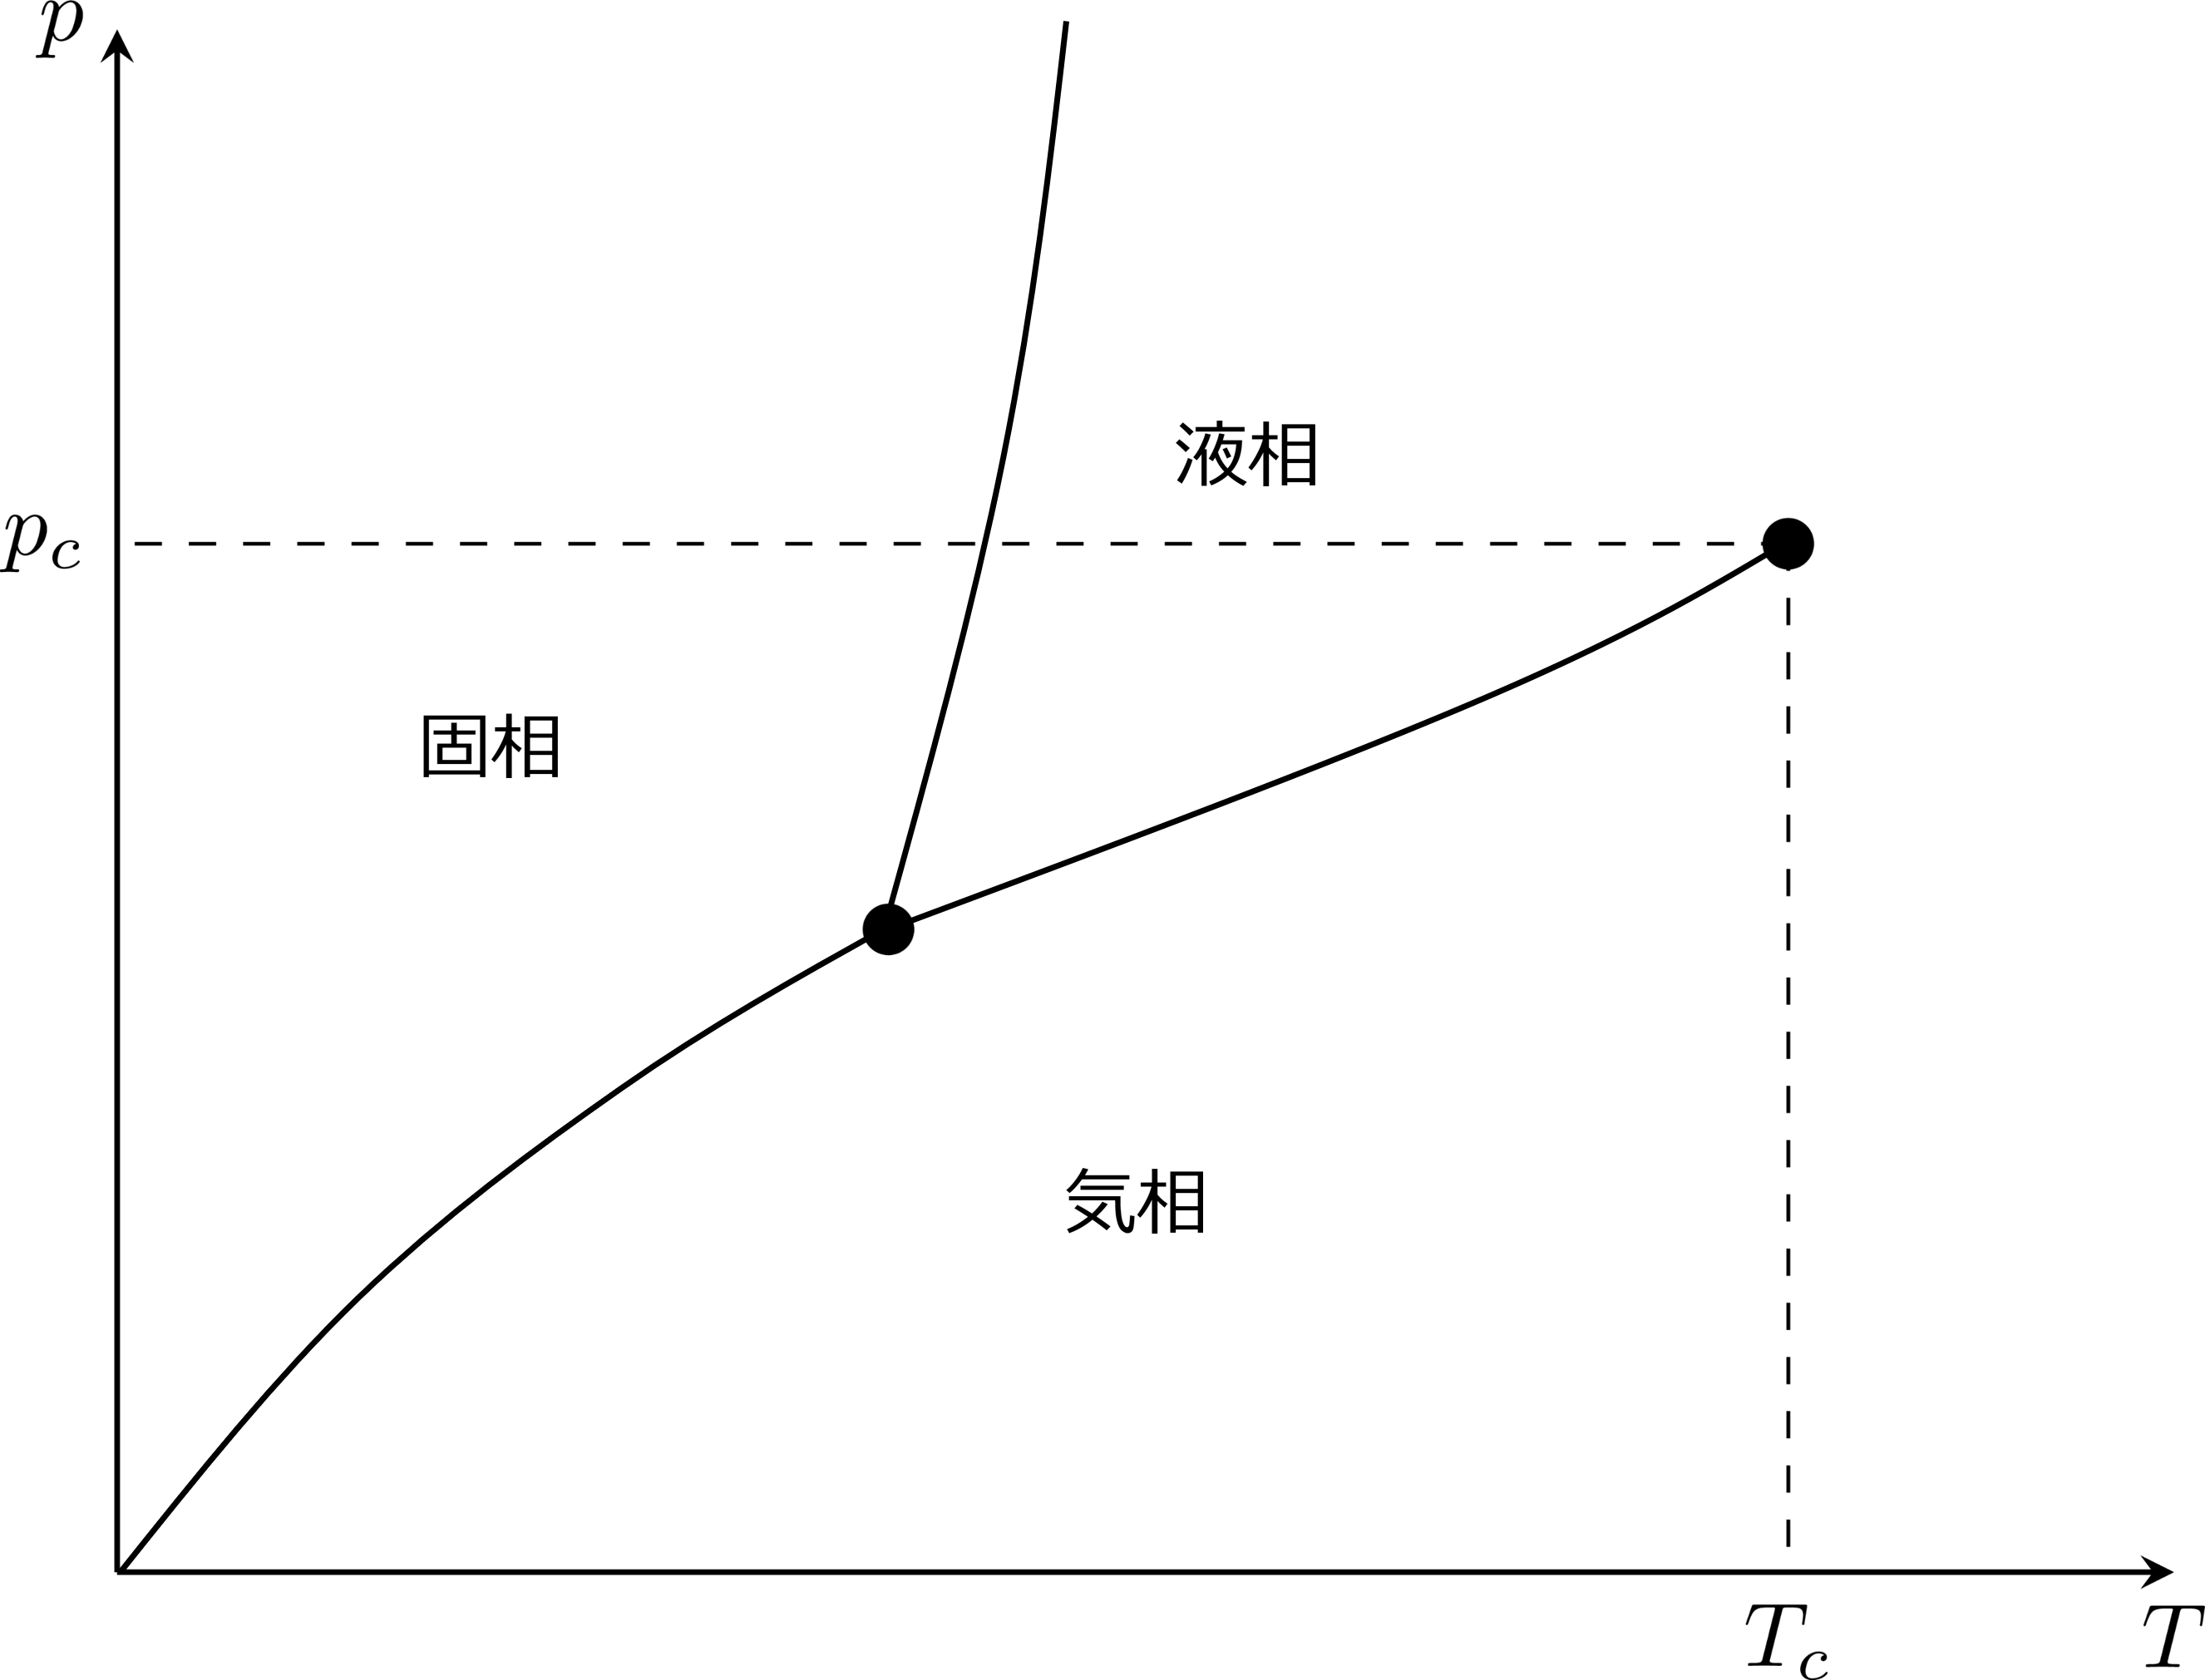
\includegraphics[height=7cm]{image/三態相図.png}
       \caption{典型的な三態の相図.}
       \label{三態相図}
   \end{center}
\end{figure}
なぜ同じ\ce{H2O}という物質が,温度を変えただけで,固相,液相,気相という全く性質の異なる状態をとるのか.素朴に考えれば,このような変化は水の素である\ce{H2O}分子の性質の変化からくると考えたくなる.つまり,何らかの意味での「ミクロなルール」が変化しているのではないかと想定するということである.\par
しかし,相転移が起こるのは「ミクロなルール」が変化するからではない.なぜなら,ミクロな自由である分子にとって,温度とは,周囲からくる熱的なノイズの平均値を決定するためのパラメータにすぎず,それによってミクロな分子の形状や相互作用が不連続に変化するなど決してありえないからである.\par
「ミクロなルール」が不変であっても,系を構成する要素(今の場合,水分子)の数がきわめて大きければ,それら相互の関連が変化することで,マクロな性質の不連続な変化が生じうる.つまり,相転移は,無数の要素が複雑に絡み合ったときに全体として生じる協力現象の一種なのである.\par
図\ref{三態相図}は典型的な純物質の相図の模式図である.絶対温度$T$と圧力$p$を変化させると,相図の境界を横切るときに相転移が生じ,例えば物質の密度や比熱が不連続に変化する.境界線で仕切られる三つの領域が固相,液相,気相である.\par
しかし,図\ref{三態相図}を見ると,液相と気相を仕切る境界線が途中で途切れている.つまり,この途切れている部分より右上の領域では液相と気相の区別がないのである.\par
これは,相というのが一部分に着目したときに意味を持つ「局所的」な概念であることを示唆している.どの状態をどの相と同定するかは,相図のどの部分に着目するかに応じて変わるのである.それに対して,どの部分で物理量の特異な変化が生じるかを示す相図(より正確には,パラメータ空間の中での境界の位置)は,解釈の余地なく定まっている.\par

\subsection{臨界現象とは}
相図(図\ref{三態相図})で液相と気相を仕切る線が消えてしまう点$(T_c,p_c)$を臨界点(critical point)とよぶ.臨界点での温度$T_c$が臨界温度,圧力$p_c$が臨界圧力である.臨界点近傍では,臨界現象(critical phenomena)とよばれる,一連のきわめて興味深い現象がみられる.\par
臨界温度$T_c$よりも低い温度$T$では,液相と気相の区別がある.温度を$T$に保ったまま圧力を変化させ,液相から気相に移るときに密度の不連続な変化量(つまり,「とび」)を$\Delta \rho(T)$とする.$T>T_c$では液相と気相の区別がなくなることから,$T \nearrow T_c$とすれば,$\Delta \rho(T) \searrow 0$となる.しかも,このとき,密度の「とび」は
\begin{equation}
  \Delta \rho(T) \approx (T_c -T)^{\beta}, \quad T \nearrow T_c \text{のとき}
\end{equation}
という,特異な温度依存性を示すことが知られている.特異性を特徴づける指数$\beta$は,臨界指数(critical exponent)とよばれる量の一つである.\par
様々な物質について臨界指数$\beta$を調べると,面白いことに,すべての物質について
\begin{equation}
  \beta \simeq 0.325
\end{equation}
に近い値が得られる.臨界指数$\beta$は,物質に依存しない普遍的な定数である可能性が高い.もちろん,$T_c$や$p_c$の値は物質ごとに大きく異なっている.臨界現象を特徴づける臨界指数$\beta$が物質に依存しないというのは驚くべき実験事実である.このような強力な定量的普遍性の背後に何があるのかを探るには,実に魅力的な理論物理学の課題である.

\section{強磁性イジング模型}
これまで,最も身近な相転移という理由で物質の三態を扱ってきたが,実は固相,液相,気相のあいだの相転移についての理論な現状,理論的な理解は進んでいない.しかし,もう一つ我々の身近にある物質である磁石,物理学の用語で言い換えると強磁性体に関係する相転移はよく知られている.そのため,本論文では強磁性体の相転移を扱う.\par
この節では,強磁性体の相転移を調べるために,強磁性イジング模型(本論文では以降,単にイジング模型とよぶ)を定義する.イジング模型は,実在の強磁性体のモデルとしては全く忠実ではないが,強磁性体での相転移の本質をつかむためには,きわめてすぐれたモデルである.つまり,相転移や臨界現象を引き起こすために必要最低限の要素だけを持ったモデルと言える.\par
「イジング模型」という呼び名は,このモデルの一次元でのふるまいを1924年の学位論文で調べたイジングにちなんだものである.ただし,モデルの発案者は当時イジングの指導教員であったレンツである.\par
\subsection{モデルの定義}
\begin{figure}[H]
  \begin{center}
      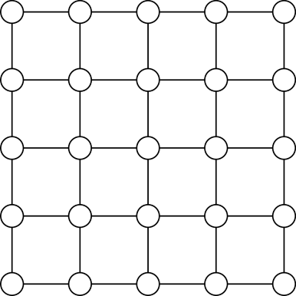
\includegraphics[height=4cm]{image/2次元格子.png}
      \caption{$d=2, L=5$の場合の格子.25個の格子点上にそれぞれスピンがのっている.線分で結ばれた2つのスピンは相互作用している.離れたスピンは直接相互作用しないが,間にあるスピンを介して,間接的に相互作用している.}
  \end{center}
\end{figure}
一辺が$L$の$d$次元立方格子を考える.全格子点の数を$N=L^d$とし,それぞれの格子点に$i=1,2,\dots ,N$と番号をつけておく.各格子点には,上向きと下向きの二つの状態をとるスピンがのっている.格子点$i$のスピンを表すスピン変数を$\sigma_i = \pm{1}$とする.$+1$が上向きスピン,$-1$が下向きスピンのに対応する.また,スピン変数$\sigma_i$に対応する物理量を$\hat{\sigma}_i$と書く.\par
系のエネルギー固有状態は,すべての格子点のスピン変数を$(\sigma_1, \sigma_2, \dots, \sigma_N)$と列挙することで指定できる,このようなスピンの並びのことをスピン配位と呼ぶ.今後,スピン配位を$\bm{\sigma}=(\sigma_1, \sigma_2, \dots, \sigma_N)$で表すことにする.それぞれのスピンが二通りの状態をとるため,系の全状態数,あるいは,スピン配位の総数は$2^N$である.スピン配位$\bm{\sigma}$に対応するエネルギー固有値を
\begin{equation}
  E(\bm{\sigma}) = -J \sum_{\langle i, j \rangle} \sigma_i \sigma_j
  - \mu_0 H \sum_{i=1}^{N} \sigma_i \label{イジングエネルギー}
\end{equation}
とする.第一項はスピン間の相互作用を表す項で,第二項は外部磁場$H$とスピン磁気モーメント$\mu_0$の相互作用を表す項である.第一項の和$\sum_{\langle i, j \rangle}$は互いに隣り合う格子点$i,j$すべてについての和という意味である.\par
ここでは相互作用定数$J$は$J>0$とする.したがって,隣り合う格子点の組$i,j$に関わる相互作用を取り出すと,
\begin{equation}
  -J \sigma_i \sigma_j =
  \begin{cases}
    -J, & \sigma_i = \sigma_j \text{のとき}    \\
    J,  & \sigma_i \neq \sigma_j \text{のとき}
  \end{cases} \label{相互作用項場合分け}
\end{equation}
となる.つまり,隣り合う格子点のスピンが揃う方がエネルギーが小さくなる.このように互いにスピンを揃えようとする相互作用を,強磁性的相互作用という.\par
このイジング模型では.1つのスピンは隣り合ったスピンと相互作用し,それ以外のスピンとは直接相互作用しない.しかし,あるスピンは隣のスピンと相互作用し,その隣のスピンとまた相互作用し,というように「伝言ゲーム」のように伝わっていく.間接的には,格子上のすべてのスピンが互いに何らかの相互作用を及ぼし合っている.

\subsection{平衡状態での物理量}
ここで,イジング模型の逆温度$\beta$での平衡状態を調べる.この場合,カノニカル分布で平衡状態を記述するのが自然である.\par
分配関数は
\begin{equation}
  Z_L(\beta, H) = \sum_{\bm{\sigma}} \exp{[-\beta E(\bm{\sigma})]} \label{イジング分配関数}
\end{equation}
である.和は$2^N$通りのすべてのスピン配位についてとる.後の便利のために格子サイズを$L$とした.物理量$\hat{g}$の期待値は
\begin{equation}
  \langle \hat{g} \rangle_{\beta, H}^{\text{can}}
  := \frac{1}{Z_L(\beta, H)}  \sum_{\bm{\sigma}} g(\bm{\sigma}) \exp{[-\beta E(\bm{\sigma})]}
\end{equation}
である.ここで,$g(\bm{\sigma})$は状態$\bm{\sigma}=(\sigma_1,\dots,\sigma_N)$における$\hat{g}$の値である.スピン一つあたりの自由エネルギーを
\begin{equation}
  f_L(\beta, H) := -\frac{1}{\beta H} \ln{Z_L(\beta, H)} \label{自由エネルギー}
\end{equation}
物理量としての磁化を
\begin{equation}
  \hat{m} := \frac{1}{N} \sum_{j=1}^{N} \mu_0 \hat{\sigma}_j
\end{equation}
と定義する.このとき,磁化の期待値は
\begin{align}
   m_L(\beta, H) &:= \langle \hat{m} \rangle_{\beta, H}^{\text{can}} \notag                                                                                       \\
   & = \frac{1}{Z_L(\beta, H)} \sum_{\bm{\sigma}} m(\bm{\sigma}) \exp{[-\beta E(\bm{\sigma})]} \notag                \\
   & = \frac{1}{Z_L(\beta, H)} \sum_{\bm{\sigma}} \frac{1}{N} \sum_{j=1}^N \mu_0 \sigma_j \exp{[-\beta E(\bm{\sigma})]} \notag      \\
   & = \frac{1}{Z_L(\beta, H)} \sum_{\bm{\sigma}} \frac{1}{\beta N} \frac{\partial}{\partial H} \exp{[-\beta E(\bm{\sigma})]}\notag \\
   & = \frac{1}{\beta N} \frac{1}{Z_L(\beta, H)} \frac{\partial}{\partial H} Z_L(\beta, H)  \notag                                                                 \\
   & = \frac{1}{\beta N}\frac{\partial}{\partial H} \ln{Z_L (\beta, H)} \notag                                                                                     \\
   & = -\frac{\partial}{\partial H} f_L(\beta, H) \label{磁化と自由エネルギーの関係式}
\end{align}
と書ける.これ以降,期待値$\langle \hat{m} \rangle_{\beta, H}^{\text{can}}$のことも,単に磁化と呼ぶ.磁化とは「系がどの程度磁石になっているか」の目安である.それに対して,「系がどの程度磁石になりやすいか」の目安になるのがゼロ磁場での磁化率は
\begin{equation}
  \chi_L(\beta) := \left.\frac{\partial m_L(\beta, H)}{\partial H}\right|_{H=0}
\end{equation}
である.
\subsection{絶対零度}
まずは,絶対零度での系のふるまいを見ていく.つまり,基底状態を求めるということである.\par
式(\ref{相互作用項場合分け})から,一つのスピンに着目すれば,$\sigma_i = \sigma_j$のときエネルギーが最小になる.したがって,相互作用項$-J\sigma_i \sigma_j$を最小化する状態は,すべてのスピンが等しくなっているときであることがわかる.つまり,すべての$i$について$\sigma_i = +1$もしくは$\sigma_i = -1$のいずれかの状態である.\par
一方,外部磁場とスピンの相互作用項$-\mu_0 H \sigma_i$を最小化する状態は,磁場の符号によって変わってくる.式(\ref{イジングエネルギー})の第二項を最小化するのは,$H>0$なら,すべての$i$について$\sigma_i=1$とした状態であり,$H<0$なら,すべての$i$について$\sigma_i=-1$とした状態である.$H=0$のときは,値は常に$0$になるため,すべてのスピン配位で最小値を与える.\par
以上をまとめると,$H \geq 0$のときはすべての$i$について,$\sigma_i=+1$としたものが基底状態となり,$H \leq 0$のときはすべての$i$について,$\sigma_i=-1$としたものが基底状態となる(図\ref{絶対零度スピン配位}).\par
\begin{figure}[h]
  \begin{center}
    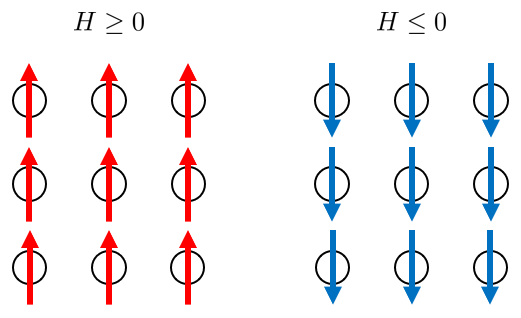
\includegraphics[height=5cm]{image/絶対零度スピン配位.png}
    \caption{絶対零度でのイジング模型の基底状態.$H>0$のときはスピンはすべて上向きになり,$H<0$のときはスピンがすべて下向きになる$H=0$のときは,これら両方の状態が基底状態になる. \label{絶対零度スピン配位}}
  \end{center}
\end{figure}
これに基づいて,絶対零度での磁化のふるまいを見てみる.すべてのスピンが$+1$の状態での磁化は$\mu_0$,すべてのスピンが$-1$の状態での磁化は$-\mu_0$なので,
\begin{equation}
  m_L(\infty, H) =
  \begin{cases}
    -\mu_0, & H \leq 0 \text{のとき} \\
    \mu_0,  & H \geq 0 \text{のとき}
  \end{cases}
\end{equation}
とわかる.(図\ref{絶対零度磁化})
\begin{figure}[h]
  \begin{center}
    \begin{tikzpicture}[scale=1]
      \draw[->,>=stealth,semithick](-3,0)--(3,0)node[below]{$H$};%x軸
      \draw[->,>=stealth,semithick](0,-2.5)--(0,2.5)node[above]{$m(\infty, H)$};%y軸
      \draw[draw=magenta,thick,domain=0:3] plot(\x,2);
      \draw[draw=magenta,thick,domain=-3:0] plot(\x,-2);
      \draw (0,0) node[below left]{0}; %原点
      \draw (0,2) node[left]{$\mu_0$};
      \draw (0,-2) node[right]{$-\mu_0$};
    \end{tikzpicture}
    \caption{絶対零度でのイジング模型の磁化のふるまい.$H=0$を境に,$-\mu_0$から$\mu_0$に不連続に変化する.\label{絶対零度磁化}}
  \end{center}
\end{figure}
つまり,磁化は$H$の関数として不連続である.もちろん,これはエネルギーを最小化する状態が入れ替わったことの単純な反映にすぎない.これに対して,同じような不連続性が$0$でない温度で見られるかどうかは,本質的に難しい問題である.

\subsection{無限体積の極限}
有限温度での相転移や臨界現象を調べるには,自由エネルギー$f_L(\beta, H)$や磁化$m_L(\beta, H)$といった物理量を計算し,それらの振る舞いを見ればよいと思える.しかし,このとき格子サイズ$L$はどの程度の大きさにとればよいのか?.実は格子サイズが有限である場合,相転移を起こさないことが示せる.ここではこれを証明する.\par
まず,格子サイズ$L$が任意の有限な整数とする.このとき,式(\ref{自由エネルギー})の形から明らかなように自由エネルギー$f_L(\beta, H)$は$\beta, H$について何度も微分できる.よって,磁化$m_L(\sigma, H)$は$H$の連続関数であることがわかる.そして,系の対称性を考える.あるスピン配位$(\sigma_1,\dots,\sigma_N)$が与えられたとき,これらすべてのスピンを反転させた新しいスピン配位を$(\tilde{\sigma}_1,\dots,\tilde{\sigma}_N)$で定義する.つまり,すべての$i$に対して$\tilde{\sigma}_i := -\sigma_i$とするということである.このとき,エネルギーの表式(\ref{イジングエネルギー})をスピン反転した変数を使って書き直せば,$\tilde{\sigma}_i \tilde{\sigma}_j = \sigma_i \sigma_j$が成り立つことを使って
\begin{equation}
  E(\bm{\sigma}) = -J \sum_{\langle i,j \rangle} \tilde{\sigma}_i \tilde{\sigma}_j -h \sum_{i=1}^{N} \tilde{\sigma}_i
\end{equation}
のように,磁場を反転させた,元のエネルギーと同じ表式が得られる.つまり,すべてのスピンを反転させることは,磁場を反転させることと等価ということである.すべての$(\sigma_1,\dots,\sigma_N)$について足し上げることは,すべての$(\tilde{\sigma}_1,\dots,\tilde{\sigma}_N)$について足し上げることと同じなので,分配関数の表式(\ref{イジング分配関数})を,
\begin{align}
  Z_L(\beta, H)
   & = \sum_{(\tilde{\sigma}_1,\dots,\tilde{\sigma}_N)} \exp{[-\beta E(\bm{\sigma})]} \notag                                                                                               \\
   & = \sum_{(\tilde{\sigma}_1,\dots,\tilde{\sigma}_N)} \exp{\left[ \beta\left( J \sum_{\langle i,j \rangle} \tilde{\sigma}_i \tilde{\sigma}_j -H \sum_{i=1}^{N} \tilde{\sigma}_i \right) \right]} \notag \\
   & = \sum_{\bm{\sigma}} \exp{\left[ \beta\left( J \sum_{\langle i,j \rangle} \sigma_i \sigma_j -H \sum_{i=1}^{N} \sigma_i \right) \right]} \notag                                         \\
   & = Z_L(\beta, -H)
\end{align}
となり,磁場を反転させても分配関数は変わらないという結果になる.自由エネルギーの定義である式(\ref{自由エネルギー})より
\begin{equation}
  f_L(\beta, H) = f_L(\beta, -H)
\end{equation}
という自由エネルギーの対称性が示せる.さらに磁化は式(\ref{磁化と自由エネルギーの関係式})より,$f_L(\beta, H)$の$H$微分で書けるので,
\begin{equation}
  m_L(\beta, H) = -m_L(\beta, -H) \label{磁化反対称性}
\end{equation}
のように書け,磁化は磁場の反転について反対称になることがわかる.\par
$f_L(\beta, H)$が微分可能なので,$m_L(\beta, H)$はすべての$\beta, H$において定義されている.よって式(\ref{磁化反対称性})で$H=0$とすれば,$m_L(\beta, 0) = -m_L(\beta, 0)$となり,$m_L(\beta, 0)=0$が得られる.したがって,有限系では$0\leq \beta < \infty$の任意の逆温度$\beta$で磁化がゼロになり,相転移を示さないことがわかる.

\section{一次元イジング模型}
一次元のイジング模型を考える.ハミルトニアンは
\begin{equation}
  H = -J \sum_{i=1}^N \sigma_i \sigma_j - h \sum_{i=1}^N \sigma_i \label{一次元イジングエネルギー}
\end{equation}
なり,周期的境界条件$\sigma_{N+1} = \sigma_{1}$を課す.分配関数は
\begin{equation}
  Z = \sum_{(\sigma_i,\dots,\sigma_N)} \exp{\left[ \beta J \sum_{i=1}^N \sigma_i \sigma_j + \beta h \sum_{i=1}^N \sigma_i \right]} \label{一次元イジング分配関数}
\end{equation}
となる.ここで,次のような対称行列$\mathrm{T}$を定義する.
\begin{equation}
  (\mathrm{T})_{\sigma_i, \sigma_{i+1}} = \exp{\left[ \beta J \sigma_i \sigma_{i+1} + \frac{\beta h}{2}(\sigma_i + \sigma_{i+1}) \right]},
\end{equation}
\begin{equation}
  \mathrm{T} = \begin{pmatrix}
    (\mathrm{T})_{1,1}  & (\mathrm{T})_{1,-1}  \\
    (\mathrm{T})_{-1,1} & (\mathrm{T})_{-1,-1}
  \end{pmatrix}=
  \begin{pmatrix}
    e^{\beta J + \beta h} & e^{-\beta J}          \\
    e^{-\beta J}          & e^{\beta J - \beta h}
  \end{pmatrix}
\end{equation}
このようにすることで,分配関数(\ref{一次元イジング分配関数})を
\begin{align}
  Z
   & = \sum_{(\sigma_i,\dots,\sigma_N)} (\mathrm{T})_{\sigma_1, \sigma_2} (\mathrm{T})_{\sigma_2, \sigma_3} \cdots (\mathrm{T})_{\sigma_N, \sigma_1} \notag \\
   & = \sum_{(\sigma_i,\dots,\sigma_N)} \prod_{i = 1}^N (\mathrm{T})_{\sigma_i, \sigma_{i+1}}
\end{align}
を書くことができる.行列の積の定義より,
\begin{equation}
  \sum_{\sigma_k = \pm{1}}(\mathrm{T}^n)_{\sigma_i, \sigma_k}(\mathrm{T}^m)_{\sigma_k, \sigma_j}
  = (\mathrm{T}^{n+m})_{\sigma_i, \sigma_j}
\end{equation}
であることを用いると,分配関数は
\begin{align}
  Z
   & = \sum_{\sigma_1 = \pm{1}}\sum_{\sigma_2 = \pm{1}} \cdots \sum_{\sigma_N = \pm{1}} (\mathrm{T})_{\sigma_1, \sigma_2} (\mathrm{T})_{\sigma_2, \sigma_3} \cdots (\mathrm{T})_{\sigma_N, \sigma_1} \notag   \\
   & = \sum_{\sigma_1 = \pm{1}}\sum_{\sigma_3 = \pm{1}} \cdots \sum_{\sigma_N = \pm{1}} (\mathrm{T}^2)_{\sigma_1, \sigma_3} (\mathrm{T})_{\sigma_3, \sigma_4} \cdots (\mathrm{T})_{\sigma_N, \sigma_1} \notag \\
   & = \sum_{\sigma_1 = \pm{1}}\sum_{\sigma_4 = \pm{1}} \cdots \sum_{\sigma_N = \pm{1}} (\mathrm{T}^3)_{\sigma_1, \sigma_4} (\mathrm{T})_{\sigma_4, \sigma_5} \cdots (\mathrm{T})_{\sigma_N, \sigma_1} \notag \\
   & = \cdots \notag                                                                                                                                                                                          \\
   & = \sum_{\sigma_1 = \pm{1}} (\mathrm{T}^N)_{\sigma_1, \sigma_1} \notag                                                                                                                                    \\
   & = \mathrm{Tr}\left[ \mathrm{T}^N \right] \label{1Dイジング分配関数トレース}
\end{align}
と表すことができる.対称行列$\mathrm{T}$は,スピン間の相互作用を次々と伝える役割を果たしているため,転送行列(transfer matrix)と呼ばれる.\par
分配関数(\ref{1Dイジング分配関数トレース})は,初等的な線形代数の知識で計算することができる.実対称であるため,転送行列$\mathrm{T}$は適当な直行行列$\mathrm{O}$を用いて,
\begin{equation}
  \mathrm{O}^{-1} \mathrm{T} \mathrm{O} =
  \begin{pmatrix}
    \lambda_{+} & 0           \\
    0           & \lambda_{-}
  \end{pmatrix}
\end{equation}
と対角化できる.転送行列$\mathrm{T}$の固有値は
\begin{equation}
  \lambda_{\pm{1}}
  = e^{\beta} \left\{ \cosh{\beta h} \pm{\sqrt{(\sinh{\beta h})^2 + e^{-4\beta J}}} \right\}
\end{equation}
より,(\ref{1Dイジング分配関数トレース})はさらに
\begin{align}
  Z
   & = \mathrm{Tr} \left[ \left\{ \mathrm{O}
  \begin{pmatrix}
      \lambda_{+} & 0           \\
      0           & \lambda_{-}
    \end{pmatrix} \mathrm{O}^{-1} \right\}^N \right] \notag   \\
   & = \mathrm{Tr} \left[
  \begin{pmatrix}
      \lambda_{+} & 0           \\
      0           & \lambda_{-}
    \end{pmatrix}^N \right] \notag                            \\
   & = (\lambda_{+})^N + (\lambda_{-})^N \label{1Dイジング分配関数}
\end{align}
と表すことができる.\par
(\ref{1Dイジング分配関数})より,スピン一つあたりの自由エネルギー$f$は
\begin{align}
  f
   & = -\frac{1}{\beta L} \ln{Z} \notag                                                                                              \\
   & = -\frac{1}{\beta L} \ln{(\lambda_{+})^N + (\lambda_{-})^N} \notag                                                              \\
   & = -\frac{1}{\beta} \ln{\lambda_{+}} - \frac{1}{\beta L} \left\{ 1 + \left( \frac{\lambda_{-}}{\lambda_{+}} \right)^{L} \right\}
\end{align}
と表すことができる.ここで,$\lambda{-}/\lambda_{+}<1$に注意して,$L \nearrow \infty$とすると,
\begin{align}
  f
   & = \lim_{L \nearrow \infty} f = -\frac{1}{\beta} \ln{\lambda_{+}} \notag                                                   \\
   & = -\frac{1}{\beta} \ln{e^{\beta} \left\{ \cosh{\beta h} \pm{\sqrt{(\sinh{\beta h})^2 + e^{-4\beta J}}}\right\}} \notag    \\
   & = -1 -\frac{1}{\beta} \ln{\left\{\cosh{\beta h} \pm{\sqrt{(\sinh{\beta h})^2 + e^{-4\beta J}}}\right\}} \label{1D自由エネルギー}
\end{align}
となり,無限体積極限での自由エネルギーを厳密に計算することができる.\par
自由エネルギーの表式(\ref{1D自由エネルギー})から,磁化を計算すると,
\begin{align}
  m(\beta, h)
   & = -\frac{\partial}{\partial h} f(\beta, h) \notag                                                                                                                                                   \\
   & = \frac{\partial}{\partial (\beta h)} \ln{\left\{ \cosh{\beta h} + \sqrt{(\sinh{\beta h})^2 + e^{-4\beta J}} \right\}} \notag                                                                       \\
   & = \frac{1}{\cosh{\beta h} + \sqrt{(\sinh{\beta h})^2 + e^{-4\beta J}}} \frac{\partial}{\partial (\beta h)}\left\{ \cosh{\beta h} + \sqrt{(\sinh{\beta h})^2 + e^{-4\beta J}} \right\} \notag        \\
   & =  \frac{1}{\cosh{\beta h} + \sqrt{(\sinh{\beta h})^2 + e^{-4\beta J}}} \left\{ \sinh{\beta h} + \frac{2\sinh{\beta h} \cosh{\beta h}}{2 \sqrt{(\sinh{\beta h})^2 + e^{-4\beta J}}} \right\} \notag \\
   & = \frac{\sinh{\beta h}}{\sqrt{(\sinh{\beta h})^2 + e^{-4\beta J}}}
\end{align}
となる.これは明らかに$\beta$と$h$について連続な関数である.特に$h=0$のとすれば$m(\beta, 0) = 0$となる.つまり,有限温度の一次元イジング模型での自発磁化は$0$であり,この系は相転移を示さないことがわかる.\par
さらに,この結果を使って磁化率$\chi(\beta)$を求めると,
\begin{align}
  \chi(\beta)
   & = \left.\frac{\partial}{\partial h} m(\beta, h)\right|_{h=0} \notag                                                                                                                                       \\
   & = \left.\frac{\partial}{\partial h} \frac{\sinh{\beta h}}{\sqrt{(\sinh{\beta h})^2 + e^{-4\beta J}}}\right|_{h=0} \notag                                                                                  \\
   & = \beta \left.\frac{\partial}{\partial (\beta h)} \frac{\sinh{\beta h}}{\sqrt{(\sinh{\beta h})^2 + e^{-4\beta J}}}\right|_{h=0} \notag                                                                    \\
   & = \beta \left.\left[ \frac{\cosh{\beta h}}{\sqrt{(\sinh{\beta h})^2 + e^{-4\beta J}}} +\frac{(\sinh{\beta h})^2 \cosh{\beta h}}{\{(\sinh{\beta h})^2 + e^{-4\beta J}\}^{3/2}} \right]\right|_{h=0} \notag \\
   & = \beta e^{2\beta J}
\end{align}
となる.$\beta J \ll 1$が成り立つ高温領域では,$\chi(\beta) \simeq \beta$となり,相互作用のない場合の振る舞い(キュリーの法則)が成り立つ.一方,低温に向かい$\beta \rightarrow \infty$となると,相互作用のない場合の磁化率との比$e^{2\beta J}$は限りなく大きくなる.これは,低温で無限個のスピンが互いにそろい合おうとすることの現れとみることができる.\par

% \section{イジング模型の平均場近似}




\begin{figure}[htbp]
  \begin{minipage}[b]{0.45\linewidth}
    \centering
    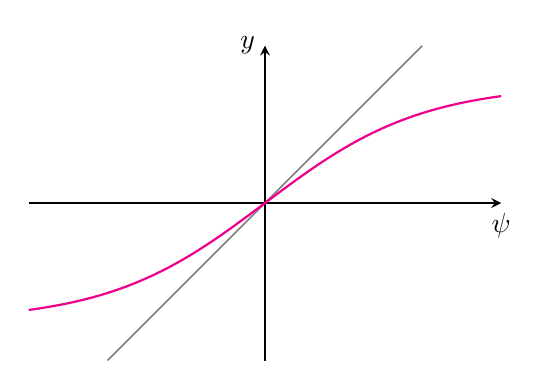
\begin{tikzpicture}[scale=1,samples=300]
      \draw[->,>=stealth,semithick](-3,0)--(3,0)node[below]{$\psi$};%x軸
      \draw[->,>=stealth,semithick](0,-2)--(0,2)node[left]{$y$};%y軸
      \draw[draw=gray,semithick,domain=-2:2] plot(\x,\x);
      \draw[draw=magenta,thick,domain=-3:3] plot(\x,{1.5*tanh(0.5*\x)});
    \end{tikzpicture}
    \subcaption{$\beta zJ \leq 1$}
  \end{minipage}
  \begin{minipage}[b]{0.45\linewidth}
    \centering
    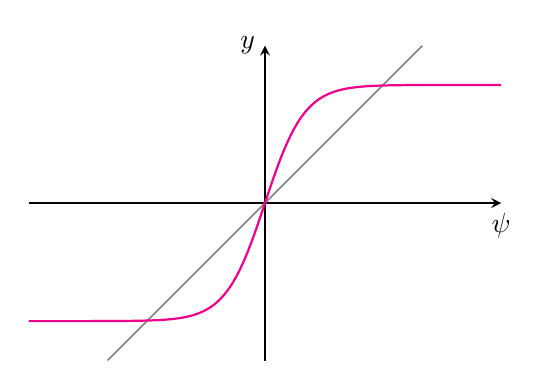
\begin{tikzpicture}[scale=1,samples=300]
      \draw[->,>=stealth,semithick](-3,0)--(3,0)node[below]{$\psi$};%x軸
      \draw[->,>=stealth,semithick](0,-2)--(0,2)node[left]{$y$};%y軸
      \draw[draw=gray,semithick,domain=-2:2] plot(\x,\x);
      \draw[draw=magenta,thick,domain=-3:3] plot(\x,{1.5*tanh(2*\x)});
    \end{tikzpicture}
    \subcaption{$\beta zJ > 1$}
  \end{minipage}
  \caption{$h=0$での自己整合方程式$\psi = \tanh{(\beta ZJ\psi)}$}
\end{figure}

\section{二次元イジング模型}
% \section{二次元イジング模型の厳密解の計算}
% 二次元イジング模型の厳密解はOnsagerによって求められた.Onsagerは,転送行列を対角化することで磁場のないときの自由エネルギーを求め,比熱をある温度で発散することを示した.いくつかの解法があるが,ここでは,高温展開を用いた解法を説明する.高温展開は,温度が高いとして自由エネルギーを$\beta J$のべきで展開する方法である.十分高温であれば,その展開を数項で打ち切って自由エネルギーの近似値とする.計算が比較的簡単なため,汎用的な手法として用いられているが,近似の正当性に十分に注意する必要がある.この近似のみを用いて相転移を調べることはできない.有限項の和から特異性が生じることはないからである.本節では,無限和を計算することにより厳密解を求め,特異性が生じることを示す.\par
% $h=0$の場合に高温展開を行う.二次元イジング模型の分配関数は
% \begin{equation}
%   Z = \mathrm{Tr}\prod_{\langle i, j \rangle} \exp{(\beta J \sigma_i \sigma_j)}
% \end{equation}
% と書ける.積はスピンの最近近接についてとる.スピン変数に関する恒等式
% \begin{align}
%   e^{x\sigma_i \sigma_j}
%    & = \frac{e^x + e^{-x}}{2} + \sigma_i \sigma_j \frac{e^x + e^{-x}}{2} \notag \\
%    & = \cosh{x} + \sigma_i \sigma_j \sinh{x}
% \end{align}
% を用いれば,
% \begin{align}
%   Z
%    & = \mathrm{Tr}\prod_{\langle i, j \rangle}(\cosh{\beta J} + \sigma_i \sigma_j \sinh{\beta J}) \notag                \\
%    & = (\cosh{\beta J})^{N_B}\mathrm{Tr}\prod_{\langle i, j \rangle}(1 + \sigma_i \sigma_j \tanh{\beta J}) \label{分配関数}
% \end{align}
% と書ける.$N_B$は最近接の数を表す.$v = \tanh{\beta J}$は有限温度で$1$より有限温度で$1$より小さい非負の量なので,(\ref{分配関数})を$v$について次のように展開する.
% \begin{equation}
%   \prod_{\langle i, j \rangle}(1 + v \sigma_i \sigma_j)
%   = 1 + v \sum_{\langle i, j \rangle} \sigma_i \sigma_j
%   + v^2 \sum_{\langle i, j \rangle, \langle k, l \rangle} \sigma_i \sigma_j \sigma_k \sigma_l + \cdots
% \end{equation}
% ここで,$\langle i, j \rangle \neq \langle k, l \rangle$である.

% \begin{equation}
%   v\sigma_i \sigma_j \longleftrightarrow
%   \begin{tikzpicture}[baseline={([yshift=-.5ex]current bounding box.center)}]
%     \draw[very thick](0,0)--(0,-1);
%     \fill(0,0)circle(0.1)node[left]{$i$};
%     \fill(0,-1)circle(0.1)node[left]{$j$};
%   \end{tikzpicture}
% \end{equation}

% \begin{equation}
%   v^2\sigma_i \sigma_j \sigma_k \sigma_l \longleftrightarrow
%   \begin{tikzpicture}[baseline={([yshift=-.5ex]current bounding box.center)}]
%     \draw[very thick](0,0)--(0,-1);
%     \draw[very thick](1,0)--(1,-1);
%     \fill(0,0)circle(0.1)node[left]{$i$};
%     \fill(0,-1)circle(0.1)node[left]{$j$};
%     \fill(1,0)circle(0.1)node[right]{$k$};
%     \fill(1,-1)circle(0.1)node[right]{$l$};
%   \end{tikzpicture}, \ \ \
%   v^2\sigma_i \sigma_j^2 \sigma_k \longleftrightarrow
%   \begin{tikzpicture}[baseline={([yshift=-.5ex]current bounding box.center)}]
%     \draw[very thick](0,0)--(0,-1);
%     \draw[very thick](0,0)--(1,0);
%     \fill(0,0)circle(0.1)node[left]{$i$};
%     \fill(0,-1)circle(0.1)node[left]{$j$};
%     \fill(1,0)circle(0.1)node[right]{$k$};
%   \end{tikzpicture}
% \end{equation}

% \begin{equation}
%   Z = (\cosh{\beta J})^{N_B}\mathrm{Tr}
%   \left[
%     1 + \sum
%     \begin{tikzpicture}[baseline={([yshift=-.5ex]current bounding box.center)}]
%       \draw[very thick](0,0)--(0,-1);
%       \fill(0,0)circle(0.1);
%       \fill(0,-1)circle(0.1);
%     \end{tikzpicture}
%     + \sum
%     \left(
%     \begin{tikzpicture}[baseline={([yshift=-.5ex]current bounding box.center)}]
%       \draw[very thick](0,0)--(0,-1);
%       \draw[very thick](1,0)--(1,-1);
%       \fill(0,0)circle(0.1);
%       \fill(0,-1)circle(0.1);
%       \fill(1,0)circle(0.1);
%       \fill(1,-1)circle(0.1);
%     \end{tikzpicture} +
%     \begin{tikzpicture}[baseline={([yshift=-.5ex]current bounding box.center)}]
%       \draw[very thick](0,0)--(0,-1);
%       \draw[very thick](0,0)--(1,0);
%       \fill(0,0)circle(0.1);
%       \fill(0,-1)circle(0.1);
%       \fill(1,0)circle(0.1);
%     \end{tikzpicture}
%     \right) + \cdots
%     \right]
% \end{equation}

% \subsection{行列を用いた定式化}
% 2次元イジング模型の厳密解に向けた前段階として,行列の観点で2次元イジング模型の定式化を行う.$n$行$n$列の正方格子上にある$N=n^2$個のスピンを考える.そして,周期的境界条件を課す.\par
% スピン座標の$\alpha$列にあるスピンをまとめて次のように表す.
% \begin{equation}
%   \mu_{\alpha}
%   \equiv \{\sigma_1, \sigma_2, \dots, \sigma_n\}
% \end{equation}
% ここで,$\mu$について次の境界条件が成り立つ
% \begin{equation}
%   \mu_{n+1} = \mu_1 
% \end{equation}
% また,スピン配位全体を$\{\mu_1, \dots, \mu_n\}$で表す.イジング模型では,$\alpha$列にあるスピンと相互作用する列は$(\alpha-1)$列と$(\alpha+1)$列のみある.そこで,$\alpha$列と$\alpha+1$列との相互作用エネルギーを$E(\mu_{\alpha}, \mu_{\alpha+1})$,$\alpha$列のスピン内でのスピン同士の相互作用エネルギーと磁場との相互作用エネルギーの総和を$E(\mu_{\alpha})$とすると,それぞれ次のようになる.
% \begin{align}
%   E(\mu, \mu')
%    & = -\epsilon \sum_{k=1}^n s_k s'_k                         \\
%   E(\mu)
%    & = -\epsilon \sum_{k=1}^n s_k s_{k+1} - H \sum_{k=1}^n s_k
% \end{align}
% ここで,$\mu$と$\mu'$はそれぞれ,隣り合った列のスピン座標の集まりである.
% \begin{align}
%   \mu  & \equiv \{s_1, \dots, s_n \} \notag \\
%   \mu' & \equiv \{s'_1, \dots, s'_n \}
%   \label{イジングエネルギー2}
% \end{align}
% 配位$\{\mu_1, \dots, \mu_n\}$における全エネルギーは
% \begin{equation}
%   E_t\{\mu_1, \dots, \mu_n \}
%   = \sum_{\alpha=1}^n [E(\mu_{\alpha}, \mu_{\alpha+1}) + E(\mu_{\alpha})]
% \end{equation}
% となり,分配関数は
% \begin{equation}
%   Z(H,T)
%   = \sum_{\mu_1} \cdots \sum_{\mu_n} \exp{\left\{ -\beta \sum_{\alpha=1}^n [E(\mu_{\alpha}, \mu_{\alpha+1}) + E(\mu_{\alpha})] \right\}}
% \end{equation}
% となる.\par
% ここで,次のように行列要素が定義された,$2^n \times 2^n$行列$\mathrm{P}$を考える.
% \begin{equation}
%   \bra{\mu} \mathrm{P} \ket{\mu'} \equiv e^{-\beta [E(\mu_{\alpha}, \mu_{\alpha+1}) + E(\mu_{\alpha})]}
%   \label{行列要素}
% \end{equation}
% これを用いると分配関数は
% \begin{align}
%   Z(H,T)
%    & = \sum_{\mu_1} \cdots \sum_{\mu_n} \bra{\mu_1} \mathrm{P} \ket{\mu_2}\bra{\mu_2} \mathrm{P} \ket{\mu_3}\cdots\bra{\mu_n} \mathrm{P} \ket{\mu_1} \\
%    & = \sum_{\mu_1}\bra{\mu_1} \mathrm{P}^n \ket{\mu_1} = \mathrm{Tr} \ \mathrm{P}^n
% \end{align}
% と$\mathrm{P}^n$のトレースで表せることがわかる.行列のトレースは行列の表現から独立しているため,上式のトレースは,以下のような対角化された$\mathrm{P}$で評価しても結果に影響を与えない.
% \begin{equation}
%   \mathrm{P} = \begin{bmatrix}
%     \lambda_1 &           &        &               \\
%               & \lambda_2 &        &               \\
%               &           & \ddots &               \\
%               &           &        & \lambda_{2^n} \\
%   \end{bmatrix}
% \end{equation}
% ここで,$\lambda_1, \lambda_2, \dots, \lambda_{2^n}$は$\mathrm{P}$の固有値である.$\mathrm{P}^n$もまた対角行列であり,対角成分は$(\lambda_1)^n, (\lambda_2)^n, \dots, (\lambda_{2^n})^n$である.したがって,分配関数は
% \begin{equation}
%   Z(H,T)
%   = \sum_{\alpha=1}^{2^n} (\lambda_\alpha)^n
% \end{equation}
% で表される.$E(\mu, \mu')$と$E(\mu)$は$n$のオーダーであるため,式(\ref{行列要素})の形式から,$n$が大きい場合,$\mathrm{P}$の固有値は一般に$e^n$のオーダーであることが予想される.$\lambda_{\text{max}}$を$\mathrm{P}$の最大固有値とすると,
% \begin{equation}
%   \lim_{n \rightarrow \infty} \frac{1}{n} \ln{\lambda}_{\text{max}}
%   = \text{finite number}
%   \label{最大固有値有限}
% \end{equation}
% と予想される.そして,もしこれが正しく,すべての固有値$\lambda_{\alpha}$が正ならば,
% \begin{equation}
%   (\lambda_{\text{max}})^n \leq Z \leq 2^n (\lambda_{\max})^n
% \end{equation}
% もしくは
% \begin{equation}
%   \frac{1}{n}\ln{\lambda_{\text{max}}}
%   \leq \frac{1}{n^2}\ln{Z}
%   \leq \frac{1}{n}\ln{\lambda_{\text{max}}} + \frac{1}{n} \ln{2}
% \end{equation}
% となる.したがって,はさみうちの原理より,
% \begin{equation}
%   \lim_{N \rightarrow \infty} \frac{1}{N} \ln{Z}
%   = \lim_{n \rightarrow \infty} \frac{1}{n} \ln{\lambda_{\text{max}}}
%   \label{n極限}
% \end{equation}
% か成り立つことがわかる.$N=n^2$.式(\ref{最大固有値有限}) が真であり,すべての固有値$\lambda_{\alpha}$が正であるという仮定が正しいことは後でわかる.したがって,$P$の最大の固有値が分かれば$n \rightarrow \infty$での分配関数が分かる.このセクションの残りの部分は,$P$の明示的な表現の説明に当てられる.


% \subsection{行列$\mathrm{P}$}
% 式(\ref{行列要素})と式(\ref{イジングエネルギー2})から我々は$\mathrm{P}$の行列要素を
% \begin{align}
%   \bra{s_1,\dots,s_n}\mathrm{P}\ket{s'_1,\dots,s'_n}
%    & = e^{-\beta[E(\mu, \mu') + E(\mu)]} \notag                                                        \\
%    & = e^{\beta \sum_{k=1}^{n}} \left( \epsilon s_k s'_k + \epsilon s_k s_{k+1} + H s_k \right) \notag \\
%    & = \prod_{k=1}^n e^{\beta H s_k} e^{\beta \epsilon s_k s_{k+1}} e^{\beta \epsilon s_k s'_k}
% \end{align}
% のように得た.ここで,$2^n \times 2^n$の3つの行列$V'_1, V_2, V_3$を定義する.それぞれ行列要素は次のように与える.
% \begin{align}
%   \bra{s_1,\dots,s_n}V'_1\ket{s'_1,\dots,s'_n}
%    & \equiv \prod_{k=1}^n e^{\beta \epsilon s_k s'_k} \label{V1}                                 \\
%   \bra{s_1,\dots,s_n}V_2\ket{s'_1,\dots,s'_n}
%    & \equiv \delta_{s_1 s'_1}\dots\delta_{s_n s'_n} \prod_{k=1}^n e^{\beta \epsilon s_k s_{k+1}} \\
%   \bra{s_1,\dots,s_n}V_3\ket{s'_1,\dots,s'_n}
%    & \equiv \delta_{s_1 s'_1}\dots\delta_{s_n s'_n} \prod_{k=1}^n e^{\beta \epsilon H s_k}       \\
% \end{align}
% ここで,$\delta_{ss'}$はクロネッカーのデルタ記号である.したがって,この表現では$V_2$と$V_3$は対角行列になる.それは簡単に示せる.
% \begin{equation}
%   \mathrm{P} = V_3 V_2 V'_1
% \end{equation}
% 行列乗算の通常の意味で,つまり
% \begin{align*}
%   & \bra{s_1,\dots,s_n}\mathrm{V}_3\mathrm{V}_2\mathrm{V}'_1\ket{s'_1,\dots,s'_n}                                                            \\
%   & = \sum_{s''_1, \dots, s''_n} \sum_{s'''_1, \dots, s'''_n} \bra{s_1,\dots,s_n}\mathrm{V}_3\ket{s''_1,\dots,s''_n} \bra{s''_1,\dots,s''_n}\mathrm{V}_2\ket{s'''_1,\dots,s'''_n}       \\
%   & \times \bra{s'''_1,\dots,s'''_n}\mathrm{V}'_1\ket{s'_1,\dots,s'_n} \\
%   & = \sum_{s''_1, \dots, s''_n} \sum_{s'''_1, \dots, s'''_n}
%   \delta_{s_1s''_1} \cdots \delta_{s_ns''_n} \delta_{s''_1s'''_1} \cdots \delta_{s''_ns'''_n} \prod_{k =1}^{n} e^{\beta H s_k} e^{\beta \epsilon s''_k s'''_{k+1}} e^{\beta \epsilon s'''_k s'_k} \\
%   & = \sum_{s''_1, \dots, s''_n} 
%   \delta_{s_1s''_1} \cdots \delta_{s_ns''_n} \prod_{k =1}^{n} e^{\beta H s_k} e^{\beta \epsilon s''_k s''_{k+1}} e^{\beta \epsilon s''_k s'_k} \\
%   & = \prod_{k =1}^{n} e^{\beta H s_k} e^{\beta \epsilon s_k s_{k+1}} e^{\beta \epsilon s_k s'_k}
% \end{align*}

% \subsection{行列の直積}
% ここで,$\mathrm{V}_3, \mathrm{V}_2, \mathrm{V}'_1$による便利な方法を述べる前に,行列の積の概念を導入する.\par
% $m \times m$の2つの行列$A, B$を考える.行列要素はそれぞれ,$\bra{i}A\ket{j}, \bra{i}B\ket{j}$である.$i, j$はそれぞれ$1, 2, \dots, m$の値をとる.このとき,直積$A \times B$は$m^2 \times m^2$の行列となり,行列要素は
% \begin{equation}
%   \bra{ii'}A \times B\ket{jj'}
%   \equiv \bra{i} A \ket{j} \bra{i'} B \ket{j'}
% \end{equation}
% と定義する.3つ以上の行列の直積$A \times B \times \cdots \times C$にも拡張でき,行列要素は
% \begin{equation}
%   \bra{ii' \cdots i''} A \times B \times \cdots \times C \ket{jj' \cdots j''}
%   \equiv \bra{i}A\ket{j} \bra{i'}B\ket{j'} \cdots \bra{i''}A\ket{j''}
% \end{equation}
% で表される.もし$AB$が通常の行列乗算のもとでの行列AとBの積を表すなら,次のようになる.
% \begin{equation}
%   (A \times B)(C \times D) = (AC) \times (BD)
% \end{equation}
% これは以下のように示せる.
% \begin{align*}
%   \bra{ii'} (A \times B)(C \times D) \ket{jj'}
%    & = \sum_{kk'} \bra{ii'} A \times B \ket{kk'} \bra{kk'} C \times D \ket{jj'} \\
%    & = \bra{i} AC \ket{j} \bra{i'} BD \ket{j'}                                  \\
%    & = \bra{ii'} (AC) \times (BD) \ket{jj'}
%   \label{直積公式}
% \end{align*}
% 式(\ref{直積公式})を一般化した,以下の等式も成り立つ.
% \begin{equation}
%   (A \times B \times \cdots \times C) (D \times E \times \cdots \times F)
%   = (AD) \times (BE) \times \cdots \times (CF)
% \end{equation}

% \subsection{スピン行列}
% ここで,$\mathrm{V}'_1, \mathrm{V}_2, \mathrm{V}_3$を便利に表現できる特別な行列をいくつか紹介する.よく知られた3つの$2 \times 2$パウリスピン行列を$X, Y, Z$とする.
% \begin{equation}
%   X \equiv \begin{pmatrix}
%     0 & 1 \\ 1 & 0
%   \end{pmatrix}, \ \ \
%   Y \equiv \begin{pmatrix}
%     0 & -i \\ i & 0
%   \end{pmatrix}, \ \ \
%   Z \equiv \begin{pmatrix}
%     1 & 0 \\ 0 & -1
%   \end{pmatrix}
% \end{equation}
% これらパウリ行列は次の関係式を満たす.\par
% \begin{equation*}
%   X^2 = Y^2 = Z^2 = 1
% \end{equation*}
% \begin{equation}
%   XY + YX = 0, \ \ YZ + ZY = 0, \ \ ZX + XZ = 0
%   \label{スピン行列性質}
% \end{equation}
% \begin{equation*}
%   XY = iZ, \ \ YZ = iX, \ \ ZX = iY
% \end{equation*}
% ここで,$2^n \times 2^n$行列$\mathrm{X}_{\alpha}, \mathrm{Y}_{\alpha}, \mathrm{Z}_{\alpha}$を定義する.
% \begin{align}
%   \mathrm{X}_{\alpha} \equiv 1 \otimes 1 \otimes \cdots \otimes \mathrm{X} \otimes \cdots \otimes 1 \notag \\
%   \mathrm{Y}_{\alpha} \equiv 1 \otimes 1 \otimes \cdots \otimes \mathrm{Y} \otimes \cdots \otimes 1        \\
%   \mathrm{Z}_{\alpha} \equiv 1 \otimes 1 \otimes \cdots \otimes \mathrm{Z} \otimes \cdots \otimes 1 \notag
% \end{align}
% $\alpha \neq \beta$のとき以下の関係式が成り立つ.
% \begin{align}
%    & [\mathrm{X}_{\alpha}, \mathrm{X}_{\beta}]
%   = [\mathrm{Y}_{\alpha}, \mathrm{Y}_{\beta}]
%   = [\mathrm{Z}_{\alpha}, \mathrm{Z}_{\beta}]
%   = 0 \notag                                   \\
%    & [\mathrm{X}_{\alpha}, \mathrm{Y}_{\beta}]
%   = [\mathrm{X}_{\alpha}, \mathrm{Z}_{\beta}]
%   = [\mathrm{Y}_{\alpha}, \mathrm{Z}_{\beta}]
%   = 0
% \end{align}
% $2^n \times 2^n$行列$\mathrm{X}_{\alpha}, \mathrm{Y}_{\alpha}, \mathrm{Z}_{\alpha}$は(\ref{スピン行列性質})のすべての関係式を満たす.

% \subsection{行列$\mathrm{V}'_1, \mathrm{V}_2, \mathrm{V}_3$}
% 式(\ref{V1})から,$\mathrm{V}'_1$が$n$個の同じ$2 \times 2$行列の直積で表せることがわかる.
% \begin{equation}
%   \mathrm{V}_1'=\bm{a} \times \bm{a} \times \cdots \times \bm{a}
% \end{equation}
% ここで,
% \begin{equation}
%   \bra{s}\bm{a} \ket{s'}
%   =e^{\beta \epsilon s s'}
% \end{equation}
% である.したがって,
% \begin{equation}
%   \bm{a}=\left[\begin{array}{cc}
%       e^{\beta \epsilon}  & e^{-\beta \epsilon} \\
%       e^{-\beta \epsilon} & e^{\beta \epsilon}
%     \end{array}\right]=e^{\beta \epsilon}+e^{-\beta \epsilon} X
%     \label{a行列}
% \end{equation}
% である.ここで,$\alpha$と$\theta$を定数として
% \begin{equation}
%   \bm{a} 
%   = \alpha e^{\theta X}
%   = \alpha (\cosh{\theta} + X \sinh{\theta})
% \end{equation}
% として,式(\ref{a行列})と係数比較すれば,
% \begin{equation}
%   \begin{cases}
%     e^{\beta \epsilon} = \alpha \cosh{\theta} \\
%     e^{- \beta \epsilon} = \alpha \sinh{\theta}
%   \end{cases}
% \end{equation}
% となり,これを解くことで
% \begin{equation}
%   \bm{a}
%   =\sqrt{2 \sinh (2 \beta \epsilon)} e^{\theta X}, \quad
%   \tanh \theta \equiv e^{-2 \beta \epsilon}
% \end{equation}
% である.したがって
% \begin{equation}
%   \mathrm{V}_1'=[2 \sinh (2 \beta \epsilon)]^{\frac{n}{2}} e^{\theta X} \otimes e^{\theta X} \otimes \cdots \otimes e^{\theta X}
% \end{equation}
% と表せる.ここで,
% \begin{align}
%   &e^{\theta X} \otimes e^{\theta X} \otimes \cdots \otimes e^{\theta X} \\
%   &= (e^{\theta X} \otimes 1 \otimes \cdots \otimes 1) (1 \otimes e^{\theta X} \otimes \cdots \otimes 1) \cdots (1 \otimes 1 \otimes \cdots \otimes e^{\theta X}) \\
%   &= e^{\theta \mathrm{X}_1} e^{\theta \mathrm{X}_2} \cdots e^{\theta \mathrm{X}_n} \\
%   &= e^{\theta\left(\mathrm{X}_1+\mathrm{X}_2+\cdots+\mathrm{X}_n\right)}
% \end{align}
% と表せることを使う.2つ目の等式では$1 \otimes \cdots \otimes e^{\theta X} \otimes \cdots \otimes 1 = e^{\theta (1 \otimes \cdots \otimes X \otimes \cdots 1)}$を使った.これより,$\mathrm{V}'_1$は次のように書ける.
% \begin{align}
%   \mathrm{V}_1'
%    & =[2 \sinh (2 \beta \epsilon)]^{\frac{n}{2}} \mathrm{~V}_1                               \\
%   \mathrm{V}_1
%    & =\prod_{\alpha=1}^n e^{\theta \mathrm{x}_{\alpha}}, \quad \tanh \theta \equiv e^{-2 \beta \epsilon}
% \end{align}
% 同様な考えより,$\mathrm{V}_2, \mathrm{V}_3$に関しても,
% \begin{align}
%   \mathrm{V}_2
%    & =\prod_{\alpha=1}^n e^{\beta \epsilon \mathbf{Z}_\alpha \mathbf{Z}_{\alpha+1}}                      \\
%   \mathrm{~V}_3
%    & =\prod_{\alpha=1}^n e^{\beta H \mathbf{Z}_\alpha} \quad, \quad \mathbf{Z}_{n+1} \equiv \mathbf{Z}_1
% \end{align}
% が示せる.したがって
% \begin{equation}
%   \mathrm{P}
%   = [2 \sinh (2 \beta \epsilon)]^{\frac{n}{2}} \mathrm{V}_3 \mathrm{V}_2 \mathrm{V}_1
%   \label{行列P最終形態}
% \end{equation}
% と表すことができる.$H=0$のとき,つまり$V_3 = 1$のとき,2次元イジング模型を完全に定式化できる.

% \subsection{数学的余談}
% 磁場がない場合の2次元イジング模型の解法に関連する,一般的なクラスの行列の研究を以下に示す.\par
% 次の反交換関係を満たす$2n$個の行列$\Gamma_{\mu} (\mu = 1,\dots,2n)$を定義する.
% \begin{equation}
%   \{\Gamma_{\mu}, \Gamma_{\nu}\}
%   =\Gamma_{\mu} \Gamma_{\nu} + \Gamma_{\nu} \Gamma_{\mu} 
%   = 2\delta_{\mu \nu}
%   \label{ガンマ反交換}
% \end{equation}

% \begin{enumerate}[(a)]
%   \item $\Gamma_{\mu}$の次元は$2^n \times 2^n$より小さくならない
%   \item もし,$\Gamma_{\mu}$と$\Gamma'_{\mu}$が\ref{ガンマ反交換}を満たす組ならば,$\Gamma_{\mu} = \mathrm{S} \Gamma'_{\mu} \mathrm{S}^{-1}$となる正則行列$\mathrm{S}$が必ず存在する.
%   \item すべての$2^n \times 2^n$行列は,単位行列,ガンマ行列$\Gamma_{\mu}$,およびガンマ行列の積$\Gamma_{\mu} \Gamma_{\nu}, \Gamma_{\mu} \Gamma_{\nu} \Gamma_{\lambda}, \cdots$の線形結合で表せる.
% \end{enumerate}
% $n=1$のとき,\ref{ガンマ反交換}を満たすのは$2 \times 2$パウリスピン行列である.すべての$2 \times 2$行列が単位行列とパウリスピン行列の線形結合で表せることは明らかである.また,$n=2$のときはすべての$4 \times 4$のDirac行列$\gamma_{\mu}$となる.\par
% $2^n \times 2^n$行列の可能な$\{\Gamma_{\mu}\}$の表現は次のようなものである.
% \begin{align*}
%   \Gamma_1 &= \mathrm{Z}_1 & \Gamma_2 &= \mathrm{Y}_1 \\
%   \Gamma_3 &= \mathrm{X}_1 \mathrm{Z}_2 & \Gamma_4 &= \mathrm{X}_1 \mathrm{Y}_1 \\
%   \Gamma_5 &= \mathrm{X}_1 \mathrm{X}_2 \mathrm{Z}_2 & \Gamma_6 &= \mathrm{X}_1 \mathrm{X}_2 \mathrm{Y}_1 \\
%   &\vdots & &\vdots
% \end{align*}
% つまり,
% \begin{align}
%   \begin{split}
%     \Gamma_{2\alpha-1} &= \mathrm{X}_1 \mathrm{X}_2 \cdots \mathrm{X}_{\alpha-1} \mathrm{Z}_{\alpha} \quad (\alpha=1,\dots,n) \\
%     \Gamma_{2\alpha} &= \mathrm{X}_1 \mathrm{X}_2 \cdots \mathrm{X}_{\alpha-1} \mathrm{Y}_{\alpha} \quad (\alpha=1,\dots,n)
%   \end{split}
% \end{align}

% \subsection{厳密解}
% 磁場がない,つまり$H=0$の場合,行列$\mathrm{P}$は
% \begin{align}
%   \mathrm{P}
%   &= [2 \sinh (2 \beta \epsilon)]^{\frac{n}{2}} \mathrm{V}_2 \mathrm{V}_1 \notag \\
%   &\equiv [2 \sinh (2 \beta \epsilon)]^{\frac{n}{2}} \mathrm{V}
%   \label{行列P磁場ゼロ}
% \end{align}
% となる.ここで,$\mathrm{V} = \mathrm{V}_1 \mathrm{V}_2$とした.
% 式(\ref{n極限})より,
% \begin{align}
%   \lim_{N \rightarrow \infty} \frac{1}{N} \ln{Z(0, T)} 
%   &= \lim_{n \rightarrow \infty} \frac{1}{n} \ln{\left\{[2 \sinh{2 \beta \epsilon}]^{\frac{n}{2}}\Lambda\right\}} \notag \\
%   &= \frac{1}{2} \ln{[2 \sinh{2 \beta \epsilon}]}
%   + \lim_{n \rightarrow \infty} \frac{1}{n} \ln{\Lambda}
% \end{align}
% となる.ここで,$\Lambda$は$\mathrm{V} = \mathrm{V}_1 \mathrm{V}_2$の最大固有値である,$\mathrm{V}_1$は式(\ref{?}),$\mathrm{V}_1$は(\ref{?})で与えられる.これらの式は,$\mathrm{V}$の固有値がすべて正で,$\lim_{n \rightarrow \infty} n^{-1}\ln{\Lambda}$が存在する場合に成り立つ.したがって行列$\mathrm{V}$を対角化を考えればよい.

% \subsection{スピン代数による$\mathrm{V}$の表現}
% 式(\ref{?})より,
% \begin{align}
%   \Gamma_{2\alpha}\Gamma_{2\alpha-1} 
%   &= (\mathrm{X}_1 \mathrm{X}_2 \cdots \mathrm{X}_{\alpha-1} \mathrm{Y}_{\alpha}) (\mathrm{X}_1 \mathrm{X}_2 \cdots \mathrm{X}_{\alpha-1} \mathrm{Z}_{\alpha}) \notag \\
%   &= (\mathrm{X}_1)^2 (\mathrm{X}_2)^2 \cdots (\mathrm{X}_{\alpha-1})^2 \mathrm{Y}_{\alpha} \mathrm{Z}_{\alpha} \notag \\
%   &= \mathrm{Y}_{\alpha} \mathrm{Z}_{\alpha} \notag \\
%   &= i \mathrm{X}_{\alpha}
% \end{align}
% \begin{align}
%   \Gamma_{2\alpha+1}\Gamma_{2\alpha} 
%   &= (\mathrm{X}_1 \mathrm{X}_2 \cdots \mathrm{X}_{\alpha} \mathrm{Z}_{\alpha+1}) (\mathrm{X}_1 \mathrm{X}_2 \cdots \mathrm{X}_{\alpha-1} \mathrm{Y}_{\alpha}) \notag \\
%   &= (\mathrm{X}_1)^2 (\mathrm{X}_2)^2 \cdots (\mathrm{X}_{\alpha-1})^2 \mathrm{X}_{\alpha} \mathrm{Z}_{\alpha+1} \mathrm{Y}_{\alpha} \notag \\
%   &= \mathrm{X}_{\alpha} \mathrm{Z}_{\alpha+1} \mathrm{Y}_{\alpha} \notag \\
%   &= \mathrm{X}_{\alpha} \mathrm{Y}_{\alpha} \mathrm{Z}_{\alpha+1} \notag \\
%   &= i \mathrm{Z}_{\alpha} \mathrm{Z}_{\alpha+1}
% \end{align}
% \begin{align}
%   \Gamma_1\Gamma_{2n} 
%   &= \mathrm{Z}_1 (\mathrm{X}_1 \mathrm{X}_2 \cdots \mathrm{X}_{\alpha-1} \mathrm{Y}_n) \notag \\
%   &= -i \mathrm{Z}_1 \mathrm{Z}_n (\mathrm{X}_1 \mathrm{X}_2 \cdots \mathrm{X}_n) \notag \\
%   &\equiv -i \mathrm{Z}_1 \mathrm{Z}_n \mathrm{U}
% \end{align}
% これより
% \begin{equation}
%   \mathrm{V_1}
%   = \prod_{\alpha=1}^{n} e^{\theta \mathrm{X}_{\alpha}}
%   = \prod_{\alpha=1}^{n} e^{-i \theta \Gamma_{2\alpha} \Gamma_{2\alpha-1}}
% \end{equation}
% \begin{align}
%   \mathrm{V}_2
%   &= \prod_{\alpha=1}^{n} e^{\beta \epsilon \mathrm{Z}_{\alpha} \mathrm{Z}_{\alpha+1}} \notag \\
%   &= \left[ \prod_{\alpha=1}^{n-1} e^{\beta \epsilon \mathrm{Z}_{\alpha} \mathrm{Z}_{\alpha+1}} \right] e^{\beta \epsilon \mathrm{Z}_n \mathrm{Z}_1} \notag \\
%   &= e^{\beta \epsilon \mathrm{Z}_n \mathrm{Z}_1} \left[ \prod_{\alpha=1}^{n-1} e^{\beta \epsilon \mathrm{Z}_{\alpha} \mathrm{Z}_{\alpha+1}} \right] \notag \\
%   &= e^{i \beta \epsilon \mathrm{U} \Gamma_1 \Gamma_{2n}} \prod_{\alpha=1}^{n-1} e^{-i \beta \epsilon \Gamma_{2\alpha+1} \Gamma_{2\alpha}} 
% \end{align}
% したがって,$\phi = \beta \epsilon$として
% \begin{equation}
%   \mathrm{V} \equiv \mathrm{V}_1 \mathrm{V}_2
%   = e^{i \beta \epsilon \mathrm{U} \Gamma_1 \Gamma_{2n}}\left[ \prod_{\alpha=1}^{n-1} e^{-i \beta \epsilon \Gamma_{2\alpha+1} \Gamma_{2\alpha}} \right] \left[ \prod_{\lambda=1}^{n} e^{-i \theta \Gamma_{2\lambda} \Gamma_{2\lambda-1}} \right]
% \end{equation}
% ここで,いくつか$\mathrm{U}$の性質を書く
% \begin{enumerate}[(a)]
%   \item $\mathrm{U}^2 = 1, \quad \mathrm{U}(1 + \mathrm{U}) = 1 + \mathrm{U}, \quad \mathrm{U}(1 - \mathrm{U}) = -(1 - \mathrm{U})$
%   \item $\mathrm{U} = i^n \Gamma_1 \Gamma_2 \cdots \Gamma_{2n}$
%   \item $\{\mathrm{U}, \Gamma_{\mu}\} = 0$
% \end{enumerate}
% これらの性質を用いることで
% \begin{align}
%   e^{i \phi \Gamma_1 \Gamma_{2n}}
%   &= \left[\frac{1}{2} (1 + \mathrm{U}) + \frac{1}{2} (1 + \mathrm{U})\right]\left[\cosh{\phi} + i \Gamma_1 \Gamma_{2n} \sinh{\phi}\right]
%   \notag \\
%   &= \frac{1}{2} (1 + \mathrm{U})\left[\cosh{\phi} + i \Gamma_1 \Gamma_{2n} \sinh{\phi}\right]
%   + \frac{1}{2} (1 - \mathrm{U})\left[\cosh{\phi} - i \Gamma_1 \Gamma_{2n} \sinh{\phi}\right] \notag \\
%   &= \frac{1}{2} (1 + \mathrm{U}) e^{i \phi \Gamma_1 \Gamma_{2n}}
%   + \frac{1}{2} (1 - \mathrm{U}) e^{-i \phi \Gamma_1 \Gamma_{2n}}
% \end{align}
% したがって
% \begin{equation}
%   \mathrm{V} 
%   = \frac{1}{2} (1 + \mathrm{U}) \mathrm{V}^+
%   + \frac{1}{2} (1 - \mathrm{U}) \mathrm{V}^-
% \end{equation}
% \begin{equation}
%   \mathrm{V}^{\pm}
%   \equiv e^{\pm i \phi \mathrm{U} \Gamma_1 \Gamma_{2n}}\left[ \prod_{\alpha=1}^{n-1} e^{-i \phi \Gamma_{2\alpha+1} \Gamma_{2\alpha}} \right] \left[ \prod_{\lambda=1}^{n} e^{-i \theta \Gamma_{2\lambda} \Gamma_{2\lambda-1}} \right]
% \end{equation}

\chapter{機械学習と深層学習}
ここでは,イジング模型に対して機械学習,深層学習による手法を応用する上で必要となる機械学習と深層学習の基礎知識について説明する.
\section{学習とは}
機械学習(Machine Learning)とはデータ分析の一種で,人間が行う知的作業を計算機に実行させる手法のことを意味する.機械学習では,データセットのみを機械(コンピュータ)に与えることでデータセットの中に潜むパターンや特徴を自動で``学習''することができる.\par
機械が学習を行うため,機械学習と名付けられているわけだが,``学習''とは何かをきちんと定式化する必要がある.さまざまな定式化が存在するが,ここでは,T. M. ミッチェル(Tom Michael Mitchell)の書籍\cite{Tom1997Machine}で書かれている有名な定式化を紹介する.次の文章はその書籍に書かれている学習の定義の部分をそのまま日本語訳したものである.
\begin{quote}
  ``コンピュータプログラムが,ある種のタスクTとパフォーマンス評価尺度Pにおいて,経験Eから学習するとは,タスクTにおけるその性能をPによって評価した際に,経験Eによってそれが改善されている場合である.''
  \hfill T. M. ミッチェル
\end{quote}
ここで,タスクTは解きたい問題,パフォーマンス評価尺度Pは精度や誤差率などの評価指標のこと,経験Eはデータセットのことを指す.\par
この内容をもう少しかみ砕いて説明する.機械学習では,学習を行うための``モデル''を構築する必要がある.機械学習の分野でモデルとは,多数のパラメータを持った非線形関数
\begin{equation}
  f_{\bm{\theta}}(\bm{x}), \quad \bm{\theta} = \{ \theta_1, \theta_2, \theta_3, \cdots \}
\end{equation}
のことを指す.モデルのパラメータすべてを何かしらの値$\bm{\theta}^* = \{ \theta_1^*, \theta_2^*, \theta_3^*, \cdots \}$と決めてしまえば,入力データ$\bm{x}$を与えたときになにかしらの出力$\bm{y}=f_{\bm{\theta}^*}(\bm{x})$を返すようになる.つまり,モデルの出力結果は関数の形とパラメータの値によって決まるということである.\par
我々は,モデルに対してデータを入力したときに,タスクをこなせるような正しい結果を出力させるようにモデルのパラメータの値を適切に設定する必要がある.これをパラメータ最適化とよぶ,この作業を機械学習では機械に行わせる.\par
パラメータ最適化のおおまかな流れを説明する.まず,パラメータの初期値を乱数を用いてランダムに決め,データ入力する.当然この状態で返ってくる出力結果は本来出力してほしい正解の値からは外れた値が帰ってくる.そこで,出力と正解の誤差を測るような評価基準を決めておき,算出された評価結果を良くするようにモデルのパラメータを更新してあげることによってモデルを改善する.再びデータを入力して,評価結果からパラメータ更新を行う.この流れを繰り返し行うことで,モデルを改善を何度も行う.そうすることで最終的には正解に近い出力結果を得られるモデルを作成する.これがパラメータ最適化の大まかな流れである.ここで注目してほしいのは,機械学習ではモデルのパラメータ最適化を機械に行わせているという点である.\par
そして,パラメータ最適化を行うことこそが機械学習における``学習''なのである.学習についての細かい説明は3.3章以降で説明する.
\begin{figure}[H]
  \begin{center}
    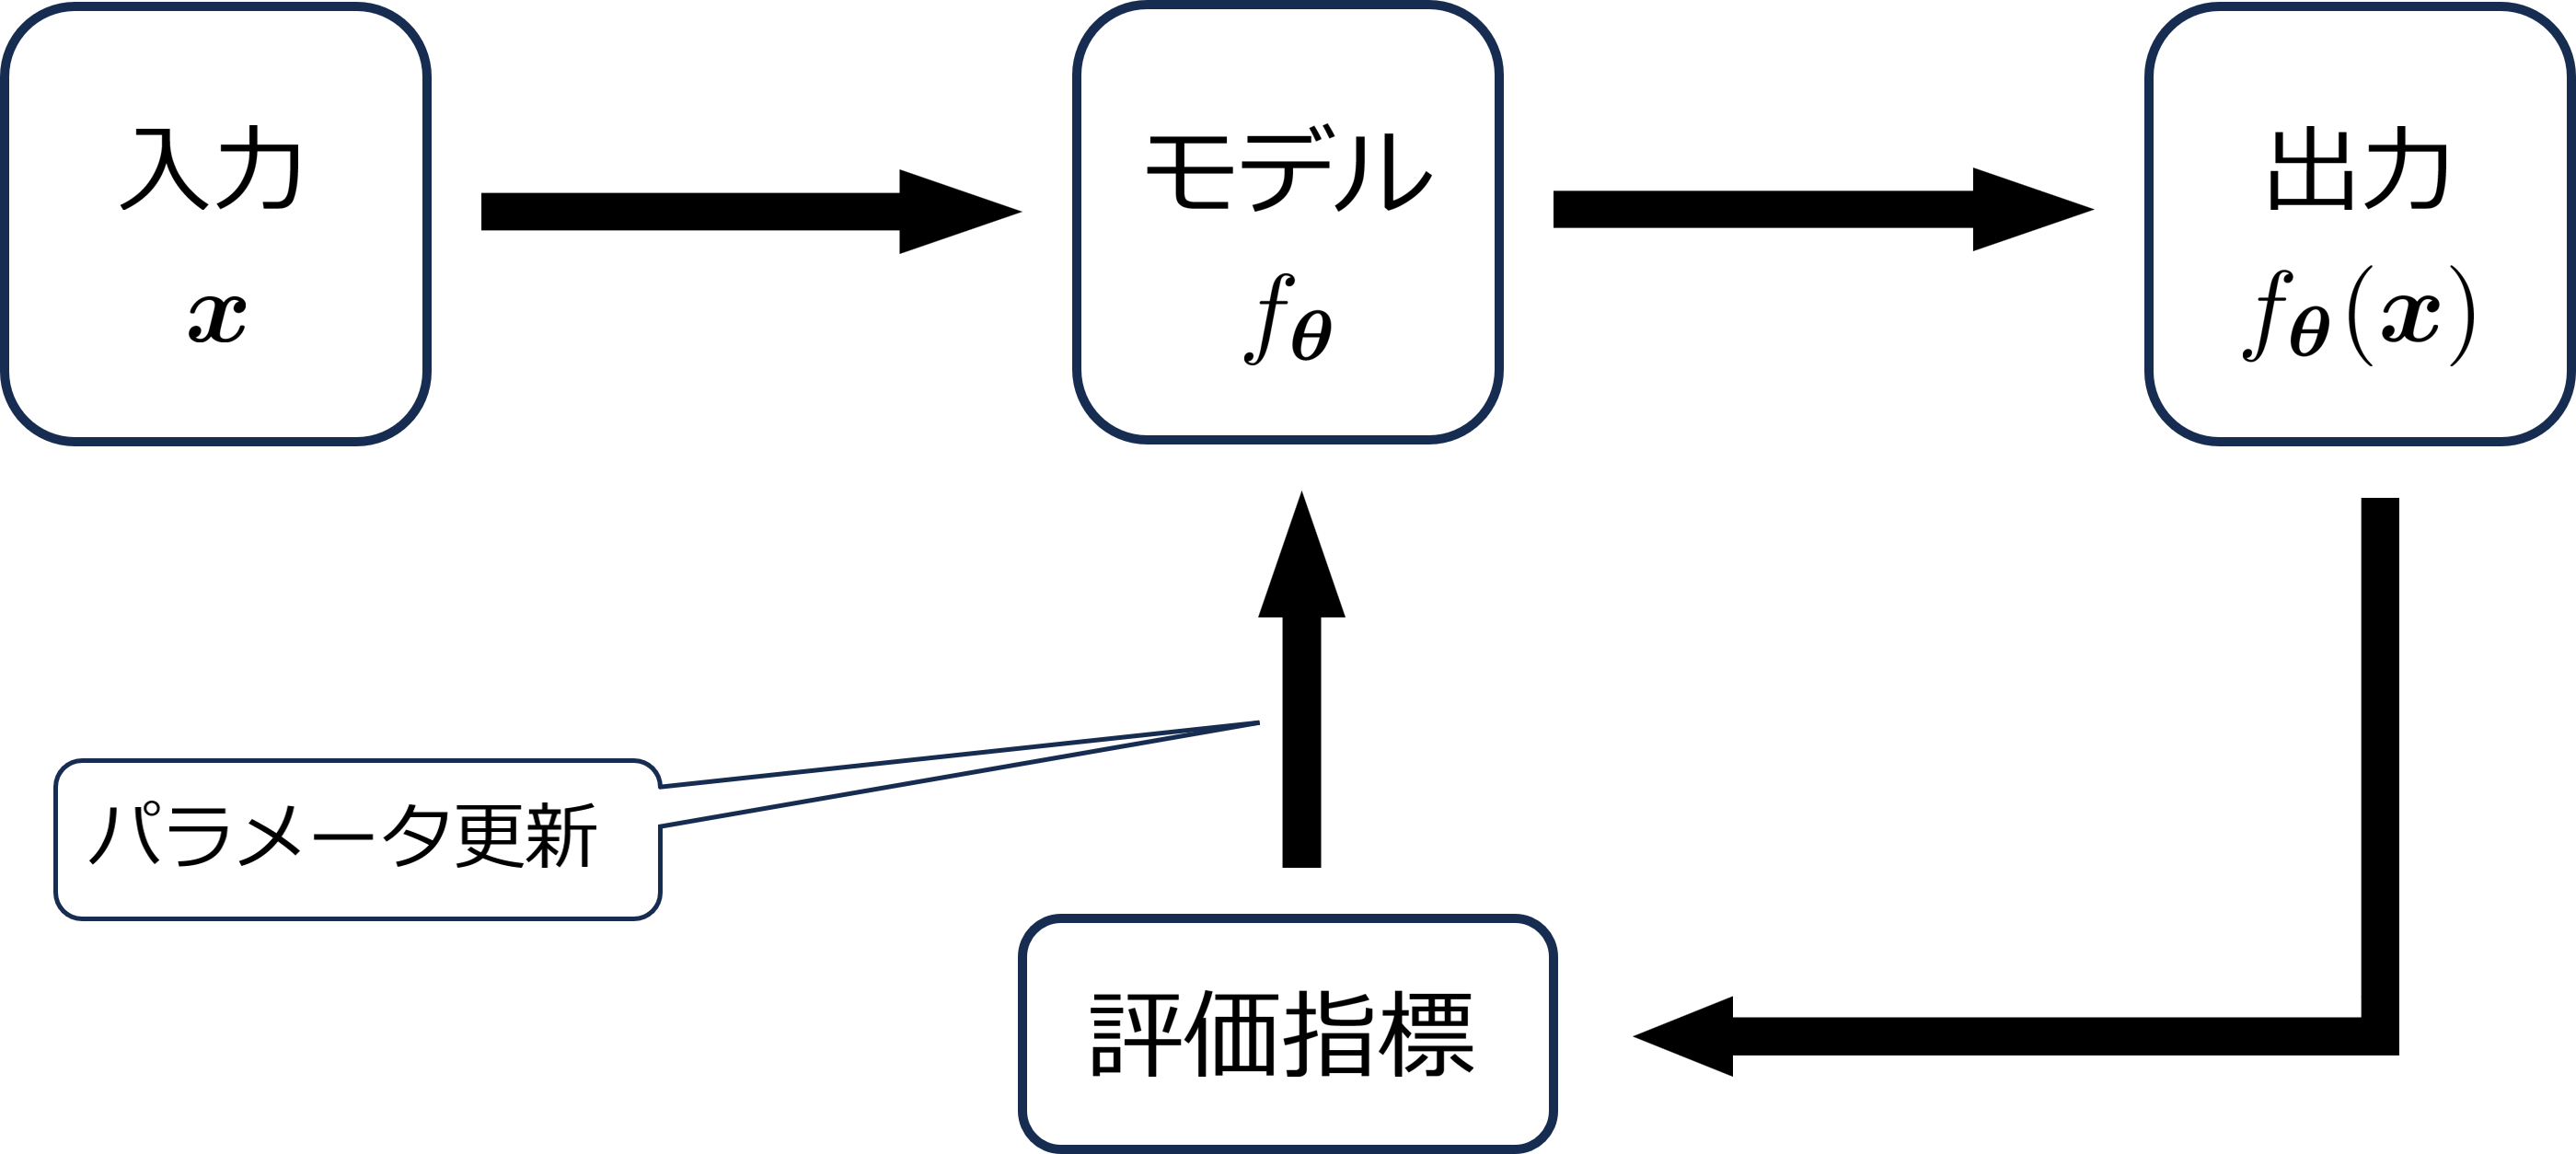
\includegraphics[height=4cm]{image/機械学習概要図.png}
    \caption{機械学習における学習の大まかな流れ}
  \end{center}
\end{figure}

\subsection{代表的なタスク}
機械学習におけるタスク,つまり解きたい問題にはどのようなものがあるか.ここでは代表的な例である「クラス分類」と「回帰」について説明する.
\subsubsection*{クラス分類}
まずクラス分類について説明する.機械学習の分野における分類(classification)とは,データをいくつかのクラスに仕分ける作業のことである.簡単な例として,送られてきた電子メールをみて,それがスパムメールか通常メールを判別するような作業を考える.これは「スパムメールor通常メール」という2つのクラスに分類するため,2クラス分類と呼べる.スパムメールを$C_0$,通常メールを$C_1$とラベル付けし,入力データを$\bm{x}$とすれば\footnote{機械学習では文章や画像データなど様々なデータを扱うが,これらのデータは基本的にベクトルの形で表現できる.},この2クラス分類というのは,与えられた$\bm{x}$が$C_0$と$C_1$のどちらに属するかを決定する作業であると言える.さらに数値的な変数$y = 0, 1$を導入すると,$\bm{x}$をクラス$C_{y}$へ分類するということは,$\bm{x}$の所属クラスを表す離散ラベル$y(\bm{x})$の値を決めることであると言い換えられる.\par
\begin{equation}
  \bm{x} \longrightarrow y(\bm{x}) \in \{0, 1\}
\end{equation}
分類先のクラスが多数にわたる場合は多クラス分類と呼ばれる.例えば分類先を「仕事」「家族」$\cdots$「友人」と複数($K$個)のファルダに分ける場合,分類先が$C_1,C_2,\cdots,C_K$となり,ラベル$y(\bm{x})$も$1$から$K$の整数値をとる.\par
\begin{equation}
  \bm{x} \longrightarrow y(\bm{x}) \in \{1, 2, \cdots, K\}
\end{equation}
\subsubsection*{回帰}
次に回帰(regression)について説明する.回帰とは,データからそれに対応する実数値ベクトル$\bm{y}$を予測する作業のことである.例えば,過去数日の気象データ$\bm{x}$から明日の気温を予測したとき,$y$は温度の数値に相当し,連続的な実数値をもつ変数になる.つまり,回帰とは,与えられた$\bm{x}$を,対応する$\bm{y}$に変換するために関数$\bm{y}(\bm{x})$を決定する作業である.
\begin{equation}
  \bm{x} \longrightarrow \bm{y}(\bm{x}) \in \mathbb{R}
\end{equation}

\subsection{データセットの例}
機械学習ではデータセットを用いて学習を行うと説明したが,具体的にどのようなデータセットが用いられるか説明だけではわかりづらいだろう.そこで,ここでは機械学習でよく用いられる有名なデータセット,MNIST,CIFAR-10,ImageNetについて紹介する.
\subsubsection*{MNIST}
\begin{figure}[H]
  \begin{center}
      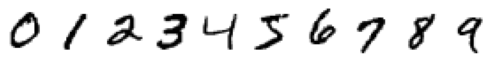
\includegraphics[height=1.8cm]{image/mnist.png}
      \caption{MNISTデータセットの一部}
      \label{MNIST}
  \end{center}
\end{figure}
0から9までの整数の手書き文字データセット.機械学習のプログラミング実装のチュートリアルとして0から9までの整数を機械に分類させるというタスクを行うのが王道になっており,このときに使われるデータベースがMNISTである.MNISTデータベース(Mixed National Institude of Standards and Technology database)はアメリカの国立標準技術研究所(NIST),昔の国立標準局が提供した手書き数字のデータベースをシャッフルして作られたデータ集合である(図\ref{MNIST}).国勢調査局職員と高校生から集められた手書き数字の画像データが訓練用に6万枚,テスト用に1万枚用意されている.それぞれのサンプルはグレースケールの$28 \times 28$ピクセル画像に整えられている.

\subsubsection{CIFAR-10}
\begin{figure}[H]
  \begin{center}
      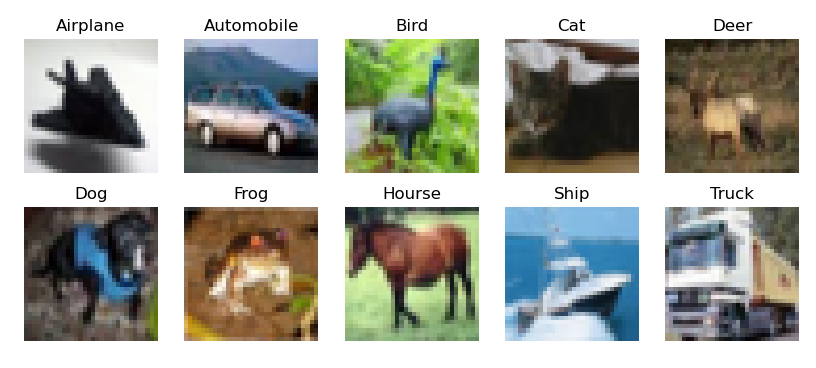
\includegraphics[height=6cm]{image/CIFAR10.png}
      \caption{CIFAT-10データセットの一部}
      \label{CIFAR10}
  \end{center}
\end{figure}
MNISTデータセットによる手書き数字の分類の次のステップとして自然画像の分類を機械学習で実装することが多い,このときチュートリアルとしてよく用いられるのがCIFAR-10である.CIFAR-10は10のカテゴリに分けられた$32 \times 32$ピクセルの自然画像のデータセットである(図\ref{CIFAR10}).訓練用画像6万枚とテスト用画像1万枚からなる.

\subsubsection{ImageNet}
ImageNetは,約1400万枚の自然画像からなる巨大なデータベースである.各画像に対して,写っている物体1つのカテゴリの正解ラベルがつけられており,クラス数は2万にも及ぶ.このデータベースは写真に写っている特定の物体を分類させる物体カテゴリ認識や,一般の画像に写っている物体を検出させて,さらにそれらを分類させる物体検出などのタスクを行う機械学習モデルを開発するために用意されたものである.

\section{統計入門}
機械学習では,データ(経験)をもとにしてプログラムがいろいろなタスクをこなせるようにさせることが目標である.ではどのようにしたらプログラムはデータからタスクをこなすための知識を学びとれるか.それを理解するにはデータを科学的に分析する数理的手法である統計学の知識が必要である.ここでは,統計の基礎を確認し,どのようにして学習アルゴリズムやパフォーマンス評価尺度を設計できるかについて説明する.
\subsection{標本と推定}
まず,データ(集合)やサンプル,標本という用語についてきちんと定めておく.これらはデータ点の集まりからなる.画像データの例でいえば,データというのは統計分析に用いるために用意した画像の集合のことで,1枚1枚の画像のことをデータ点と呼ぶ.ただし,実際はデータ点も略してデータと呼んだり,さらにはサンプルをサンプルの要素であるデータ点の意味でも用いられたりする.つまり,これらは用語の乱用でされている.そのため,本論文でも文脈に応じてこの使い方に準じることにする.\par
データ点(サンプル)の集まりからなるデータを分析するのが統計である.ここでは「推定」について考える.例として,日本人の平均身長の値を知りたい場合,これを正確に測るにはすべての日本人(母集団)の身長を調べて,それの平均を求めればよい.しかし,それは現実的に不可能である.そのため,母集団の中から十分な数だけランダムに選び取った(抽出した)日本人の身長データを集めて,その平均値をすべての日本人の平均身長であると推定するのである.つまり,「推定」というのは母集団からランダムに抽出\footnote{データの要素を1つ取り出すことは,正確には抜き取りという.}されたデータのみを用いて分析し,母集団についての知識を獲得することを指すのである.\par
統計学では母集団の性質はデータ生成分布$P_{\text{data}}({x})$により特徴づけられているものと仮定する.つまり,不確実性を伴う現象を確率的にモデル化するのである.なぜモデル化が必要なのかというと,我々が手にするデータは自然界の様々な物理的過程を経て存在しているわけだが,その過程すべてを人間には認識することは不可能であるからである.そのため,データを何らかの確率論的な過程したがってランダムに生じているとみなしているのである.例として「サイコロを振ってどの目が出るか」という試行を考えてみる.もしサイコロやその周囲のすべての物理的情報を把握できるのであれば,原理的には出る目は力学で計算できるはずである.しかし人間には有限の認識・計算能力しかないため,どの目も1/6の確率で出るようにしか見えない.そのため,私たちはサイコロを振るという行為を,どの目も出る確率が1/6である確率現象とみなしているのである.このように確率的にモデル化することでさまざまな現象を確率論的に予測することができる.\par
ここで,$\bm{x}$という具体的なサンプルはデータ生成分布から抽出されたものであると仮定したとき,ある確率変数$\mathrm{x}$の実現値$x$がデータ生成分布$P(\mathrm{x})$から抽出されたことを
\begin{equation}
  \bm{x} \sim P_{\text{data}}(\mathbf{x})
\end{equation}
と表す
\footnote{抽出について1つ注意が必要である.それは,抽出されたデータは基本的に無作為抽出によって得られたもの.つまり,すべてのサンプルは同一分布から独立に抽出されたものとする点である.なぜなら,我々は母集団について知りたいため,サンプルの抽出方法によって,結果に偏りが生じてしまっては困るからである.}.\par
したがって母集団について知識を得るということは,データ生成分布を知ることを意味する.データを特徴づける十分な統計量をパラメータと呼ぶ.実際にはデータの生成の過程は極めて複雑なため,本当の$P(\mathrm{x})$は無数のパラメータをもっており,分布を完全に知ることはほぼ不可能である.そこで通常は$P(\mathrm{x})$をよく近似できると期待できるモデル分布$P(\mathrm{x};\bm{\theta})$を仮定し,そのモデルのパラメータ$\bm{\theta}$の最適値$\bm{\theta}^*$をデータから推定する.これはパラメトリックはアプローチと呼ばれる.パラメトリックなモデルを仮定したことで,分布を特徴付ける少数のパラメータの値を推定すればよいことになる.このようにデータ生成の過程について推論できれば,その結果を使うことで新規のデータに関してもいろいろと予測することができる.
\subsection{点推定}
点推定とは,手持ちの有限個要素のデータ集合$\mathcal{D} = \{ x_1, x_2,\dots, x_N \}$からパラメータの尤もらしい値を推定する手法である.点推定では,データを決める確率変数$\{ \mathrm{x}_1, \mathrm{x}_2, \dots, \mathrm{x}_N \}$の関数である推定量
\begin{equation}
  \hat{\bm{\theta}}( \mathrm{x}_1, \mathrm{x}_2, \dots, \mathrm{x}_N )
\end{equation}
を作る.推定量そのものも確率変数であるため,データが具体的に与えられて,はじめてパラメータの推定値
\begin{equation}
  \hat{\bm{\theta}}^*( x_1, x_2, \dots, x_N )
  =\hat{\bm{\theta}}( x_1, x_2, \dots, x_N )
\end{equation}
を与えることになる.この推定値が,いま考えているパラメータをよく近似するように推定量を作れれば.データの数値から,背後にある分布について知ることができる.\par
よい推定量の作り方にはいくつもの指標がある.そこで,ここでは推定量に推奨される性質をいくつか紹介する.

\subsubsection*{バイアスが小さい}
推定量の期待値$\mathrm{E} \left[ \hat{\bm{\theta}} \right]$と真の値$\bm{\theta}^*$との差
\begin{equation}
  b(\hat{\bm{\theta}})
  = \mathrm{E} \left[ \hat{\bm{\theta}} \right] - \bm{\theta}^*
\end{equation}
のことをバイアスという.ここでの期待値は,データ生成分布での期待値なので,たくさんのデータ集合を用意して計算した平均値である.バイアスが小さいとは,推定量の偏りが小さく真の値から不要にズレていないということである.特にバイアスがゼロのものを不偏推定量と呼び,典型的な望ましい推定量である.一方でバイアスがあるものの,データの数が増えるにつれゼロへ漸近する状況$\lim_{N \rightarrow \infty} b(\hat{\bm{\theta}}) = 0$を漸近不偏推定量と呼ぶ.

\subsubsection*{分散が小さい}
分散は,真の値に対してどれだけ推定量がばらつくかを測っている.したがって,これが小さいことは望ましいのは明らかである.
\begin{equation}
  \text{Var}\left( \bm{\theta} \right)
  = \mathrm{E} \left[ \left( \hat{\bm{\theta}} - \bm{\theta} \right)^2 \right]
\end{equation}

\subsubsection*{一致性}
一致性とは,データ点の数を増えるにつれて統計量が真のパラメータに近づいていくという性質である.つまり,$N \rightarrow \infty$に従い
\begin{equation}
  \hat{\bm{\theta}}
  \rightarrow \bm{\theta}^*
\end{equation}
となるということである.この性質を満たす推定量を一致推定量と呼ぶ.

\subsubsection{ガウス分布の場合}
点推定の例としてガウス分布を考える.ガウス分布とは実数値をとる確率変数$\mathrm{x}$上の次のような分布である.
\begin{equation}
  P(\mathrm{x})
  = \mathcal{N}(\mathrm{x}; \mu, \sigma^2)
  = \frac{1}{\sqrt{2 \pi \sigma^2}} e^{-\frac{(\mathrm{x}-\mu)^2}{2\sigma^2}}
\end{equation}
この場合,$\bm{\theta} = \{ \mu, \sigma^2 \}$であり,$\mu$は平均,$\sigma^2$は分散を表している.したがってこの2つのパラメータが決ればこの分布が定まる.では,ガウス分布から無作為に取り出した$N$個のデータからパラメータ$\{ \mu, \sigma^2 \}$を推定するにはどうすればよいか?\par
まず,$\mu$の推定量$\hat{\mu}$について考える.今,どのサンプルも無作為に抽出されているとしたため,任意のデータ点$\mathrm{x}_n$はガウス分布に従う独立な確率変数である.したがって,その期待値は
\begin{align}
  E_{\mathcal{N}}[\mathrm{x}_n]
  &= \int_{-\infty}^{\infty} x_n P(x_n) dx_n \notag \\
  &= \frac{1}{\sqrt{2 \pi \sigma^2}} \int_{-\infty}^{\infty} x_n e^{-\frac{(x - \mu)^2}{2\sigma^2}} dx_n \notag \\
  &= \frac{1}{\sqrt{2 \pi \sigma^2}} \int_{-\infty}^{\infty} ({x'}_n + \mu) e^{-\frac{{x'}_n^2}{2\sigma^2}} dx'_n \notag \\
  &= \frac{\mu}{\sqrt{2 \pi \sigma^2}} \int_{-\infty}^{\infty} e^{-\frac{{x'}_n^2}{2\sigma^2}} dx'_n \notag \\
  &= \mu
\end{align}
となり,分布のパラメータ$\mu$に一致していることがわかる.
そこで,$\mu$の推定量$\hat{\mu}$を,与えられたデータ$\mathcal{D} = \{ x_1, x_2, \dots, x_N \}$に関する平均値
\begin{equation}
  \hat{\mu}
  = \frac{1}{N} \sum_{n=1}^{N} \mathrm{x}_n
\end{equation}
とする.そうすると,この推定量の期待値は
\begin{equation}
  E_{\mathcal{N}}[\hat{\mu}]
  = \frac{1}{N} \sum_{i=1}^N \mathrm{E}[\mathrm{x}_n] = \mu
\end{equation}
と見事に$\mu$と一致し,不変推定量になっていることがわかる.\par
次に$\sigma^2$の推定量はどう決めればよいか?$\sigma^2$の期待値を計算してみると
\begin{align}
  \mathrm{E}_{\mathcal{N}}[(\mathrm{x}_n - \mu)^2]
   & = \int_{-\infty}^{\infty} (x_n - \mu)^2 P(x_n) dx_n \notag \\
   & = \frac{1}{\sqrt{2 \pi \sigma^2}}\int_{-\infty}^{\infty} {x'}_n^2 e^{-\frac{{x'}_n^2}{2 \sigma^2}} dx'_n \notag \\
   & = \sigma^2
\end{align}
となることから,安直には$\mu$のときと同様に,サンプル平均
\begin{equation}
  \hat{\sigma}^2
  = \frac{1}{N} \sum_{n=1}^N (\mathrm{x}_n - \hat{\mu})^2
\end{equation}
を用いればよいと思う.しかし,これの期待値を計算すると
\begin{align*}
  \mathrm{E}_\mathcal{N}\left[\hat{\sigma}^2\right]
   & =\mathrm{E}_\mathcal{N}\left[\frac{1}{N} \sum_{n=1}^N\left(\mathrm{x}_n-\hat{\mu}\right)^2\right]                                                                                                                                       \\
   & =\frac{1}{N} \mathrm{E}_\mathcal{N}\left[\sum_{n=1}^N\left\{\left(\mathrm{x}_n-\mu\right)^2-2\left(\mathrm{x}_n-\mu\right)(\hat{\mu}-\mu)+(\hat{\mu}-\mu)^2\right\}\right]                                                                       \\
   & =\frac{1}{N}\left\{\sum_{n=1}^N \mathrm{E}_\mathcal{N}\left[\left(\mathrm{x}_n-\mu\right)^2\right]-2 \sum_{n=1}^N \mathrm{E}_N\left[\left(\mathrm{x}_n-\mu\right)(\hat{\mu}-\mu)\right]+N \mathrm{E}_N\left[(\hat{\mu}-\mu)^2\right]\right\}                       \\
   & =\sigma^2-\frac{2}{N^2} \sum_{n=1}^N \sum_{m=1}^N \mathrm{E}_\mathcal{N}\left[\left(\mathrm{x}_n-\mu\right)\left(\mathrm{x}_m-\mu\right)\right]+\frac{1}{N^2} \sum_{n=1}^N \sum_{m=1}^N \mathrm{E}_\mathcal{N}\left[\left(\mathrm{x}_n-\mu\right)\left(\mathrm{x}_m-\mu\right)\right] \\
   & =\sigma^2-\frac{1}{N^2} \sum_{n=1}^N \mathrm{E}_\mathcal{N}\left[\left(\mathrm{x}_n-\mu\right)^2\right]                                                                                                                                 \\
   & =\sigma^2-\frac{1}{N} \sigma^2                                                                                                                                                                              \\
   & =\left(1-\frac{1}{N}\right) \sigma^2
\end{align*}
となり,不偏推定量ではないという結果になる.ただし,$N \rightarrow \infty$の極限でこの期待値は$\sigma^2$に一致するため,漸近的不偏推定量になっている.余分な係数を除けば,バイアスがゼロになるため
\begin{equation}
  \hat{\tilde{\sigma}}^2 
  = \frac{1}{N - 1} \hat{\sigma^2} = \frac{1}{N - 1} \sum_{n=1}^N (\mathrm{x}_n - \hat{\mu})^2
\end{equation}
とすれば不変推定量が得られる.

\subsubsection{ベルヌーイ分布の場合}
次にベルヌーイ分布の場合を考える.ベルヌーイ分布とはコイン投げの結果が表裏どちらかなど,2つのランダムな値をとる現象を記述する分布である.確率変数を0か1の離散値をとるものとし,$\mathrm{x}$が1をとる確率を$p$とすると,この分布は,
\begin{equation}
  P(\mathrm{x}) = p^\mathrm{x} (1 - p)^{1-\mathrm{x}}
\end{equation}
と書ける.このときパラメータは$p$のみである.ベルヌーイ分布の期待値と分散は,
\begin{equation}
  \mathrm{E}_{P}[\mathrm{x}] 
  = \sum_{\mathrm{x} = 0,1} x P(x) 
  = 1 \cdot P(1) 
  = p
\end{equation}
\begin{align}
  \mathrm{E}_{P}[(\mathrm{x} - p)^2] 
  &= \sum_{\mathrm{x} = 0,1} (x -2px + p^2) P(x) \notag \\
  &= p^2 \cdot P(0) + (1 - 2p + p^2) \cdot P(1) \notag \\
  &= p(1-p)
\end{align}
であるため,パラメータの推定量は再びサンプル平均
\begin{equation}
  \hat{p} 
  = \frac{1}{N} \sum_{n=1}^N x_n
\end{equation}
がよさそうである.実際,
\begin{equation*}
  \mathrm{E}_{P}[\hat{p}] 
  = \frac{1}{N} \sum_{N=1}^{n} E_P[\mathrm{x}_n]  
  = p
\end{equation*}
となり,不変推定量であることがわかる.\par
では,分散はどうなるか?期待値を計算してみると
\begin{equation}
  \mathrm{E}\left[ (\hat{p} - p)^2 \right]
  = \frac{1}{N^2} \sum_{n=1}^{N} \mathrm{E}_{P} \left[ (x_n - p)^2 \right] 
  = \frac{1}{N} p(1 - p)
\end{equation}
となり,データサイズが大きくなるほど推定値のばらつきがゼロに近づいていく,したがって大きなデータに対して分散は小さくなるような推定量である.

\subsection{最尤推定}
点推定では発見的な方法で推定量を探してきたが,これでは複雑な分布の場合に推定量を見つけることができない.ところがパラメトリックな場合には,実は広く使える強力な手法がある.それが最尤推定法である.\par
データ生成分布のパラメトリックモデル$P_{\text{model}}(\mathrm{x}; \bm{\theta})$が与えられているとする.与えられたサンプル$\mathcal{D} = \{x_1, x_2, \dots, x_N\}$は,この分布から無作為に抽出されていると近似する.すると,これらは独立に同じモデルから生成された実現値であるため,このデータ集合が得られる同時確率は
\begin{equation*}
  P(x_1, x_2, \dots, x_N; \bm{\theta}) 
  = \prod_{n=1}^N P_{\text{model}}(x_n; \bm{\theta})
\end{equation*}
である.これを変数$\bm{\theta}$に対する量とみなして$L(\bm{\theta}) = P(x_1, x_2, \dots, x_N; \bm{\theta})$と書き,尤度または尤度関数と呼ぶ.データ値が$\{ x_1, x_2, \dots, x_N \}$という観測値を取ったのは,パラメータ$\bm{\theta}$の値が確率$P(x_1, x_2, \dots, x_N; \bm{\theta})$を大きくするようなものであったからであると考える.つまり,$L(\bm{\theta})$を最大にするようなパラメータ値であるためにデータ$\{ x_1, x_2, \dots, x_N \}$が実現されやすかったと解釈するのである.すると,与えられたデータに対して尤もらしいパラメータの値は尤度を最大化したものということになる.
\begin{equation}
  \bm{\theta}_{ML} = \underset{\bm{\theta}} {\operatorname{argmax}} L(\bm{\theta})
\end{equation}
ただし,尤度は確率の積であるため,1以下の数値を何回も掛け合わせた値になる.値が小さすぎると計算機上でアンダーフローを起こしうるため,実用上,対数尤度を最大化する.\par
\begin{equation}
  \bm{\theta}_{ML} = \underset{\bm{\theta}} {\operatorname{argmax}} (\ln{L(\bm{\theta})})
\end{equation}
尤度と対数尤度のどちらで最大化を行っても結果は変わらないことか明らかである.機械学習ではこのように何らかの目的関数を最大化,もしくは最小化することで推定に用いる最適なパラメータ値を決定するのがほとんどである.実際,多くの機械学習アルゴリズムは最尤法を基礎に構築される.ただし,実際の機械学習では,最大値よりも最小値をして問題を書く場合が多いため,負の対数尤度を目的関数とした最小化問題として表現する.
\begin{equation}
  \bm{\theta}_{ML} = \underset{\bm{\theta}} {\operatorname{argmin}} (-\ln{L(\bm{\theta})})
\end{equation}

\subsubsection{ガウス分布の場合}
ガウス分布で最尤推定法を考える.$N$個のデータに対する尤度は
\begin{equation}
  L(\bm{\theta})
  = \prod_{n=1}^N \frac{1}{\sqrt{2 \pi \sigma^2}} e^{-\frac{(x_n - \mu)^2}{2 \sigma^2}}
\end{equation}
である.ただし,$\bm{\theta} = (\mu, \sigma^2)$とした.対数尤度は
\begin{equation}
  \ln{L(\bm{\theta})}
  = -\frac{N}{2} \ln{\sigma^2} - \sum_{n} (x_n - \mu)^2 + \text{const.}
\end{equation}
となる.この関数の最大値を探すには,微分係数がゼロの場所を求めればよいので,
\begin{align}
& \left.\frac{\partial \ln L(\bm{\theta})}{\partial \mu}\right|_{\bm{\theta}_{ML}}
= \frac{1}{\sigma_{M L}^2} \sum_{n=1}^N\left(x_n-\mu_{M L}\right) = 0 \\
& \left.\frac{\partial \ln L(\bm{\theta})}{\partial \sigma^2}\right|_{\bm{\theta}_{ML}}
= -\frac{N}{2 \sigma_{M L}^2}+\frac{1}{2\left(\sigma_{M L}^2\right)^2} \sum_{n=1}^N\left(x_n-\mu_{M L}\right)^2 = 0
\end{align}
を解けばよい.これはすぐに解け,得られる推定量は
\begin{align}
  \mu_{ML}
  &= \frac{1}{N} \sum_{n=1}^{N} x_n \\
  \sigma_{ML}^2
  &= \frac{1}{N} \sum_{n=1}^{N} (x_n - \mu_{ML})^2
\end{align}
となる.これは推定量$(\hat{\mu}, \hat{\sigma}^2)$での推定値と等しくなっている.

\subsubsection{ベルヌーイ分布の場合}
ベルヌーイ分布に対しては,対数尤度は
\begin{equation}
  L(p) = \prod_{n=1}^{N} p^{x_n} (1 - p)^{1 - x_n}
\end{equation}
となる.よって対数尤度は
\begin{equation}
  \ln{L(p)} = \sum_{n=1}^{N} (x_n \ln{p} + (1 - x_n)\ln{(1 - p)})
\end{equation}
となる.これの微分係数がゼロの場所は
\begin{align}
  \left.\frac{\partial \ln{L(p)}}{\partial p}\right|_{p_{ML}}
  &= \left.\sum_{n=1}^{N} \left(\frac{x_n}{p} - \frac{1 - x_n}{1 - p}\right) \right|_{p_{ML}} \notag \\
  % &= \left.\sum_{n=1}^{N} \left(\frac{x_n - p}{p(1-p)}\right) \right|_{p_{ML}} \notag \\
  &= \left(\frac{\sum_n x_n - N p_{ML}}{p_{ML}(1-p_{ML})}\right)
\end{align}

を解けばよい.したがって
\begin{equation}
  p_{ML} = \frac{1}{N} \sum_{n=1}^{N} x_n
\end{equation}
となり,これもまた先ほど求めた推定量$\hat{p}$の推定値と一致している.このように最尤法は推定量を求めるための汎用性のある方法である.

\section{機械学習の基礎}
3.1章で機械学習とは何かについて定義し,大まかな学習の流れを説明した.ここでは機械学習についてもう少し踏み込んだ内容について詳しく説明していく.
% 機械学習ではデータ集合を学習アルゴリズムで処理することでコンピュータプログラムを学習させる.それによって,プログラムが与えられたタスクをよりうまくこなせるようにすることを目標にする.データ(集合)は機械学習の文脈では訓練データと呼ばれる.\par
% 学習を担うのは,人間がデザインするアーキテクチャである.そして,アーキテクチャの学習プロセスを決めているのが学習アルゴリズムで,これもまた人間が設計する.アルゴリズムの詳細は学習させたいタスクやデータの種類によって変わる.ただし,一般的な設計思想は,まず与えられたタスクに対するパフォーマンスの良さを測る尺度を導入し,その値を改善するようなアルゴリズムを実現するというものである.この評価尺度を機械学習では損失関数や誤差関数と呼ぶ.

\subsection{教師あり学習}
機械学習にはいくつもの枠組が存在しているが,大きく「教師あり学習」,「教師なし学習」,「強化学習」の3つに分類される.ここでは教師あり学習について説明する.\par
「教師あり」と「教師なし」の違いはモデルの学習に用いるデータ(訓練データとよぶ)が前者は入力値とそれに対する正解値のペアになっており,後者は入力値のみになっているという点である.したがって,教師あり学習では用意すべき訓練データが必ず入力$\bm{x}$と正解$\bm{y}$のペアの形をとっている.
\begin{equation}
  \mathcal{D} 
  = \{ (\bm{x}_1, \bm{y}_1), \dots, (\bm{x}_N, \bm{y}_N) \}  
\end{equation}
この入力と正解の間の関係を推定することで,新しい未知の$\bm{x}$が与えられたときに対応する正解$\bm{y}$を適切に予測できるようになることが教師あり学習での目的である.\par
\begin{equation}
  \bm{x} \longrightarrow \bm{y}
\end{equation}
統計学の用語を用いていえば,説明変数$\mathbf{x}$と目標変数$\mathbf{y}$の間の関係式を知り,常に目標変数を予測できるモデルを作ろうということである.そのために目標変数\footnote{目標変数には,離散値ととる確率変数である質的変数と,連続値をとる確率変数である量的変数の2種類がある}の適切な推定量$\hat{y}$を探すのが学習である.実際には推定量の関数モデルを仮定して,そのパラメータを訓練データから最適化する学習アルゴリズムを実装する.

\subsection{最小二乗法による線形回帰}
教師あり学習における回帰問題の手法として最小二乗法を用いた線形回帰について説明する.ここでは出力がベクトルではなくスカラーの場合を考える.つまり,入力$\bm{x}$から正解$y$を予想するという回帰問題を扱うということである.\par
まず,パラメトリックなモデルを考える.つまり,すべてのパラメータをまとめて$\bm{w}$としたとき,$y$は常にある関数$\hat{y} = f(\bm{x}; \bm{w})$で表される規則で$\bm{x}$が決まっているとする.このとき,パラメータ$\bm{w}$の値はまだ未知であり,与えられたデータから最適なパラメータ値を決める作業を行う.これが学習に相当する.また,データの観測には必ずノイズが生じるため,それを確率変数$\epsilon$として,
\begin{equation}
  y = f(\bm{x}; \bm{w}) + \epsilon
\end{equation}
のようにモデル化する.その一方で我々が知りたいのは$\bm{x}$と$y$の間の対応規則を捉える項$f(\bm{x}; \bm{w})$である.\par
ここで考えるのは,特に規則性の部分がパラメータの1次関数であることを仮定した回帰モデルである.
\begin{equation}
  f(\bm{x}; \bm{w})
  = \bm{w}^{\top} \bm{h}(x) 
  = \sum_{j=0} w_j h_j(\bm{x})
\end{equation}
これはパラメータに対して線形であるため線形回帰と呼ばれる.一方で$h_j(\bm{x})$は必ずしも線形関数である必要はない.例えば,入力$x$がベクトルではなくスカラーの場合,$h_j(x) = x^j$という単項式を選んでもよい.
\begin{equation}
  f(x; \bm{w}) = \bm{w}^{\top} \bm{h}(x) = \sum_{j=0}^M w_j x^j
\end{equation}
これは多項式回帰とよばれ,多項式回帰も線形回帰の一種である.\par
回帰分析ではモデル$f(\bm{x}; \bm{w})$が与えられたデータ$\mathcal{D}$の入出力が満たす対応関係によく当てはまるように,モデルのパラメータ$\bm{w}$を調整する.そのためにはモデルがどの程度データに当てはまっているかを測る尺度が必要である.機械学習では特に,誤差関数または損失関数と呼ばれるモデル$f(\bm{x}; \bm{w})$をパフォーマンスの悪さを測る尺度を最小化することにより最適パラメータ$\bm{w}^*$を決定する.誤差関数にはさまざまな種類があるが,その中で最も有名で理解しやすいのが,次のような平均二乗誤差である.
\begin{equation}
  E_{\mathcal{D}}(\bm{w})
  = \frac{1}{N} \sum_{n=1}^{N}(\hat{y}(\bm{x}_n; \bm{w}) - y_n)^2
\end{equation}
$\hat{y}(\bm{x}_n; \bm{w})$はモデルに$n$番目の入力データを入れて得られるモデル予測であり,$y_n$が実際にデータに対応した正解値である.したがって,$(\hat{y}(\bm{x}_n; \bm{w}) - y_n)^2$は予測と正解の差を2乗したものである.これはまさに予測と正解のズレを測っており,それを全サンプルについて平均したものがこの誤差関数である.そして,平均二乗誤差を最小化してパラメータ最適化を行う手法が平均二乗法である.\par
平均二乗法とは平均二乗誤差を最小化するパラメータの探索であるため,次のような最小値問題を解くことに対応する.
\begin{equation}
  \bm{w}^* = \underset{\bm{\theta}} {\operatorname{argmin}} (E_{\mathcal{D}}(\bm{w}))
\end{equation}
これを解くことで,関数$\hat{y}$から正しい出力値を得ることができるようになる.
\subsection{訓練誤差と汎化誤差}
ここで誤差関数の最小化によるパラメータ最適化を行う上で知っておきたい重要な概念を述べておく.機械学習の本来の目的は,手持ちの訓練データだけでなく,母集団すべてデータに対してよい良い出力をするモデルを作ることである.訓練データをもとにしてアーキテクチャを訓練し,訓練データにない未知のデータに対してまでよく働く状況が実現されることを汎化(generalization)という.汎化を達成するために本来最小化すべき誤差関数は本来は訓練誤差ではなく,次のような,モデルの出力と実際の正解値との差の2乗をデータ生成分布による期待値で定義した誤差である.
\begin{equation}
  E_{\text{gen}}(\bm{w}) 
  = \mathrm{E}_{(\mathbf{x}, \mathrm{y}) \sim P_{\text{data}}} \left[ (\hat{\mathrm{y}}(\mathbf{x}; \bm{w}) - y)^2 \right]
\end{equation}
これを汎化誤差とよぶ.しかしながら,有限な能力しかない我々には,可能なすべてのデータを集めてくることはできない.したがって,汎化誤差を最小化を行うことは不可能なのである.そこで機械学習では手持ちのデータのサンプル平均で汎化誤差を近似的に見積った,訓練誤差を最小化している.訓練誤差を小さくしただけでは,汎化がそう易々と実現するとはなかなか言えない.しかし驚くべきことに,訓練誤差の最小化でも,汎化を実現することは可能である.

\subsection{学習不足と過学習}
訓練誤差の最小化によって汎化を実現することは可能であることを述べたが,汎化の実現がそう簡単ではない.なぜなら,モデルのパラメータ数の設定値によって,学習不足や過学習といった汎化を妨げる現象が起こるからである.ここでは,パラメータの値によって学習不足や過学習が生じることを簡単な例を用いて説明する.\par
1次元データの多項式回帰を考える.つまり,与えられた入力$x$から出力$y$を予測する規則性を推定するために,多項式モデル
\begin{equation}
  \hat{y} = \sum_{j=0}^M w_j x^j
\end{equation}
をデータにフィッティングする.この際,多項式の次数$M$がパラメータで,値を我々が選ばなくてはならない.このようにモデルの選択時に決めなければならないパラメータのことをハイパーパラメータとよび,重みやバイアスといった学習されるパラメータとは区別する.例として,$M=2$で設定した場合,
\begin{equation}
  \hat{y} = w_2 x^2 + w_1 x + w_0  
\end{equation}
となり,これは2次関数でフィッティングするということである.
このような多項式モデルの場合,$M$を設定することで自動的に重みパラメータの個数も決定しているため,まさに$M$がモデルの自由度を与えていることが分かる.図\ref{線形回帰}は1次元データに対して$M=2, 4, 20$でフィッティングした結果である.

\begin{figure}[H]
  \begin{minipage}[b]{0.3\linewidth}
    \centering
    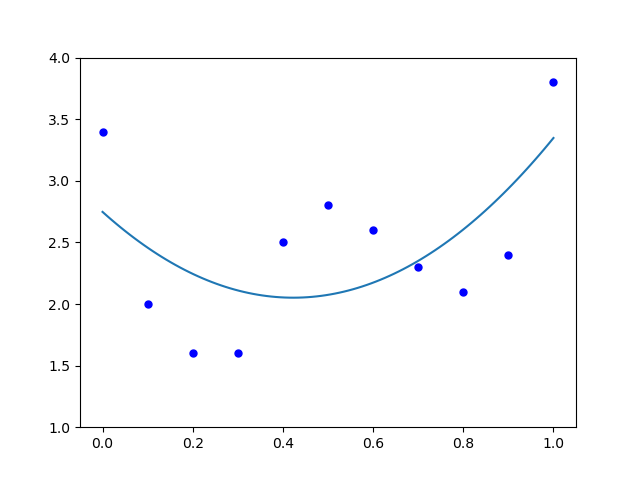
\includegraphics[keepaspectratio, scale=0.3]{image/多項式回帰(a).png}
    \subcaption{$M=2$でフィッティング}
  \end{minipage}
  \begin{minipage}[b]{0.3\linewidth}
    \centering
    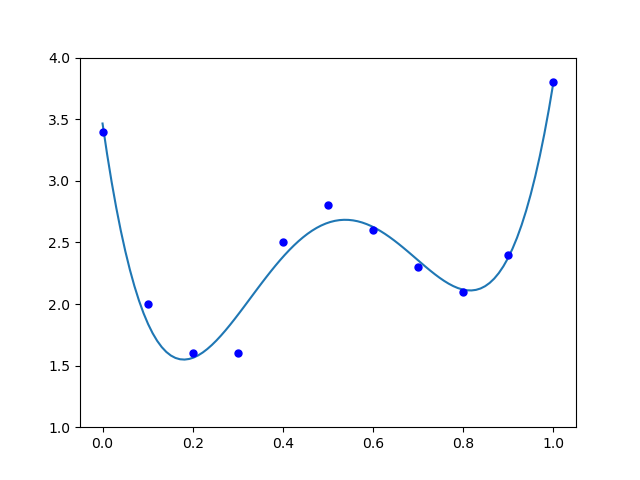
\includegraphics[keepaspectratio, scale=0.3]{image/多項式回帰(b).png}
    \subcaption{$M=4$でフィッティング}
  \end{minipage}
  \begin{minipage}[b]{0.3\linewidth}
    \centering
    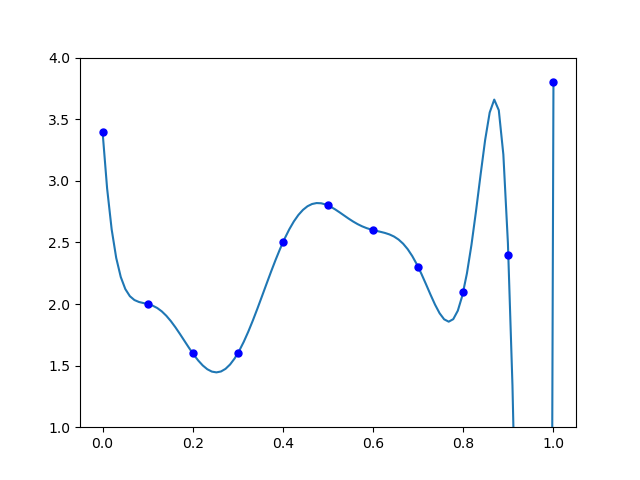
\includegraphics[keepaspectratio, scale=0.3]{image/多項式回帰(c).png}
    \subcaption{$M=20$でフィッティング}
  \end{minipage}
  \caption{1次元データの線形回帰の例.}
  \label{線形回帰}
\end{figure}

$M=2$に対応する図\ref{線形回帰}(a)のように,データに対してモデルの自由度が小さすぎると,データの構造を捉えることはまったくできない.つまり,訓練誤差の値が大きすぎて,これでは何の予測能力の得られないだろう.このような状況は学習不足またはアンダーフィッティングと呼ばれる.\par
$M$を大きくしていけば,データの複雑な構造をよりよく捉えられるようになる.しかし,不必要に大きな自由度をもったモデルは,異なる問題を引き起こす.というのも,モデルの自由度が大きすぎると,学習データのもつノイズ(統計的なゆらぎ)までも多項式モデルが正確にフィッティングしてしまうのである.図\ref{線形回帰}(c)は$M=20$でフィッティングを行った結果であり,ちょうどそのような状況になっている.与えられた訓練データに関する誤差関数に値は確かにどんどん小さくできるが,未知のデータに対してはどんどん予測能力を失っていく.図の右側はそれが顕著に表れていることがわかる.この状況は過学習またはオーバーフィッティングとよばれる.\par
このようにモデルの自由度が小さすぎると学習不足になり,逆に大きすぎると過学習になってしまうため,我々はこの間にあるちょうどよい自由度のモデルを設定する必要場ある.図(\ref{線形回帰})(b)は$M=4$でフィッティングした結果であるが.これはモデルの自由度と学習すべきデータを含む情報の豊かさがつり合っており汎化が実現していそうな良い状況であることが見てわかる.\par
このように機械学習をうまくいかせるためには,ちょうどよいモデルパラメータの数,つまりモデルの自由度を見積もらなくてはならない.自由度の見積もりにはいろいろな基準があるが,残念なことに深層学習のような複雑なモデルではどれもあまり役立たないのが現状である.そこで実務の場面では,学習に用いるデータとは別に検証用のデータ(検証データとよぶ)を用意して検証用データに関する誤差を目安に,仮定したモデルがよいものかどうかを見極めることになる.

\subsection{正則化}
過学習を避けるための一番わかりやすい方法は,自由度の数が大きすぎないモデルをはじめから選んでおくことである.自由度を実質的に減らしてしまうさまざまな手法は正則化と呼ばれる.実はモデル自体を修正することなく,学習アルゴリズムを少し変更するだけで実質的な自由度を減らすことができる.一般的にこのような正則化は,最適化すべき誤差関数の変更として表現することができる.
\begin{equation}
  E_{\text{new}}(\bm{w}) 
  = E(\bm{w}) + \lambda R(\bm{w})
\end{equation}
$\lambda$は正則化の効果の大きさを調整するための正則化パラメータである.\par
重み減衰(weight decay)はこのような正則化の代表例である.多項式回帰の例からわかるように,もし強制的に多くのパラメータの値を0に制限することができれば,はじめから調整できるパラメータが少ないため自由度を減らしたことと同じことになる.そこで最小化する誤差関数に,次のような項を加えてみる.
\begin{equation}
  E_{\text{wd}}(\bm{w}) 
  = E(\bm{w}) + \lambda \bm{w}^{\top} \bm{w}
\end{equation}
新たに項に加わった右辺全体を最小化するということは,重みベクトルのノルム$\bm{w}^{\top} \bm{w}$をできる限り小さくする解$\bm{w}^*$がより好まれるようになるということである.そのため,このように修正された後の最適解では,可能な限りの$\bm{w}$の成分がほぼゼロになっている.したがって重み減衰はモデル自体を変えずに,最小化する誤差関数へのパラメータ数を減らすペナルティ項を加える正則化である.回帰に重み減衰を適用したものはRidge回帰と呼ばれる.\par
Ridge回帰以外にも,さまざまな回帰の正則化が存在する.その一例は
\begin{equation}
  E_{\text{wd}}(\bm{w}) 
  = E(\bm{w}) + \lambda \sum_i |w_i|
\end{equation}
という誤差関数と用いるLASSO回帰である.この手法もまた,不要な重みをできるだけゼロへ近づける効果がある.\par
与えられたタスクのパフォーマンス向上という目標は維持しつつも,モデルの自由度を減らして過学習を避ける正則化の手法は,汎化性能の実現を目指す機械学習では極めて重要な位置を占める.


\subsection{クラス分類}
これまで教師あり学習の回帰問題を扱ってきた.ここでは,分類問題について考える,クラス分類とは与えられた入力$\bm{x}$を$K$個のクラス$\mathcal{C}_1, \mathcal{C}_2, \dots, \mathcal{C}_K$へ分類する作業である.これらのクラスは互いに排他的であり,1つの入力に対して必ず1つの所属先があるものとする.そして,回帰のように数値的に扱うために離散的な目標変数を導入する.導入の仕方は,分類先が2つの2クラス分類と3つ以上の多クラス分類で次のように異なる.
\subsubsection*{2クラス分類の場合}
分類先が2つしかない状況では,1つ目のクラスに属していることを$y=1$,2つ目のクラスに属していることを$y=0$として表現する2値変数$y$を用いればよい.
\subsubsection*{多クラス分類の場合}
手書き数字$0 \sim 9$のどれかを判定する場合など,分類先クラスが複数ある場合はいろいろなアプローチがあるが最もシンプルなものは,$K$個のクラスそれぞれに対応して$y = 1, 2, \dots, K$という$K$個の値をとる離散変数を用いる方法である.手書き数字の例では$K = 10$である.この変数を,ベクトルを用いた別の表現である,1-of-hot符号化に写像できる.$y$によって決まる$K$成分ベクトル
\begin{equation}
  \bm{t}(y) = \begin{pmatrix}
    t(y)_1 & t(y)_2 & \cdots & t(y)_K
  \end{pmatrix}^{\top}
\end{equation}
が1-of-hot符号化である.この手法では入力が$k$番目のクラスに属している.つまり,$y=k$であることを,第$k$成分が$t(y=k)_{k} = 1$でそれ以外の成分$t(y=k)_{l \neq k}$はすべて0であることで表現している.このような表現法をone-hot表現と呼ぶ.例えば一番のクラスに属しているのであれば,
\begin{equation}
  \bm{t}(y=1) = \begin{pmatrix}
    1 & 0 & \cdots & 0
  \end{pmatrix}^{\top}
\end{equation}
ということである.ここで,クロネッカーのデルタ記号
\begin{equation}
  \delta_{i, j} 
  = \begin{cases}
    1 & (i = j) \\
    0 & (i \neq j)
  \end{cases}
\end{equation}
を使うと,one-hot表現ベクトルの成分は
\begin{equation}
  t(y)_k = \delta_{y, k}
  \label{one-hot成分}
\end{equation}
と書くことができる.

\subsection{クラス分類へのアプローチ}
クラス分類では与えられた入力に対し,離散的な目標変数を予測したいわけだが,そのためには複数のアプローチが考えられる.

\subsubsection*{関数モデル}
関数モデルは,入力と出力の間の関係を関数としてモデル化する方法である.
\begin{equation}
  \hat{y} = y(\bm{x}; \bm{w})
\end{equation}
例えば0,1の2値をとる目標変数に対し,
\begin{equation}
  y(\bm{x}; \bm{w}) = f(\bm{w}^{\top} \bm{x} + b)
\end{equation}
というモデルを仮定すると,これは1層ニューラルネットワークになっている.

\subsubsection*{生成モデル}
関数モデルによるアプローチ以外の手法では,データを確率的に取り扱う.生成モデルではデータに潜むランダム性を同時分布$P(\bm{x}, \bm{y})$のモデル化により表現し,このモデルをデータにフィットさせる.$k$成分だけが1の$\bm{t}(\bm{y})^{\top} = \begin{pmatrix} 0 & \cdots & 0 & 1 & 0 & \cdots & 0 \end{pmatrix}$に対する$P(\bm{x}, \bm{y})$は,入力が$\bm{x}$で所属クラスが$\mathcal{C}_k$である確率を意味する.この代わりに$P(\bm{x}, \mathcal{C}_k)$をモデル化しても同じことである.\par
この確率をすべてのクラスについて求めたあと,$\bm{x}$について周辺化して$P(\bm{x})$を求めてベイズの公式を使うことで条件付き確率$P(\mathcal{C}_k | \bm{x})$を求める.$P(\mathcal{C}_k | \bm{x})$がわかれば任意のデータ$\bm{x}$がわかれば任意のデータ$\bm{x}$が各クラスに属している確率が評価でき,得られた確率の値がもっとも大きくなるクラス$\mathcal{C}_k$を$\bm{x}$の所属先と予測することになる.

\subsubsection*{識別モデル}
生成モデルではまず同時分布を得て,そこから条件付き確率分布$P(\mathcal{C}_k | \bm{x})$を計算していた.このような回りくどいことをせずに$P(\mathcal{C}_k | \bm{x})$おモデル化してデータに学習させるのが認識モデルである.予測する方法は生成モデルと同様である.

\subsection{ロジスティック回帰}
クラス分類を例にとって,識別モデルをもう少し詳しく見ていく.まずは2クラス分類から考える.この場合はクラスが2つしかないため,確率分布は$P(\mathcal{C} | \bm{x}) = P(\bm{x} | \mathcal{C}) = 1$を満たす.ここでシグモイド関数
\begin{equation}
  \sigma(u) 
  = \frac{1}{1 + e^{-u}}
  = \frac{e^u}{1 + e^u}
\end{equation}
を導入する.今考えていた,条件付き確率は
\begin{equation}
  P(\mathcal{C}_1 | \bm{x}) 
  = \sigma(u)
  \label{条件付き確率がシグモイド}
\end{equation}
とシグモイド関数で書くことができる.ここで,$u$は対数オッズと呼ばれる因子で
\begin{equation}
  u 
  = \ln{\frac{P(\mathcal{C}_1 | \bm{x})}{1 - P(\mathcal{C}_1 | \bm{x})}}
  = \ln{\frac{P(\mathcal{C}_1 | \bm{x})}{P(\mathcal{C}_2 | \bm{x})}}
\end{equation}
である.
\begin{equation}
  e^u
  = \frac{P(\mathcal{C}_1 | \bm{x})}{P(\mathcal{C}_2 | \bm{x})}
\end{equation}
がオッズ比と呼ばれ,$\mathcal{C}_1$である確率とそうでない確率の比率を表す.対数オッズが0を超えると$\mathcal{C}_1$である確率が$\mathcal{C}_2$である確率を上回ることになる.したがって対数オッズも明快な意味をもつため,確率モデルを設計する際に基本的な道具となる.\par
実際多くのクラス分類では,対数オッズ$u$が入力に関する線形関数であることを仮定した単純な確率モデルが用いられる.
\begin{equation}
  u = \bm{w}^{\top} \bm{x} + b
  \label{ロジスティック回帰}
\end{equation}
$\bm{w}$はモデルのパラメータをまとめて表したベクトルである.このモデルは統計分析においてロジスティック回帰と呼ばれ,ベルヌーイ分布の統計分析法として広く用いられている.また,ロジスティック回帰は,一般化線形モデルという重要な統計モデルの典型例である.\par
訓練データとのフィッティングには最尤法を用いる.これもまた,一般化線形モデル全般に通じる方法である.まず離散数値をとる目標変数$y$は,$y=1$が1つ目のクラス$\mathcal{C}_1$に入っている場合,$y=0$が$\mathcal{C}_2$に入っている場合を表していた.つまり,
\begin{equation}
  P(y=1 | \bm{x})
  = P(\mathcal{C}_1 | \bm{x}), \quad
  P(y=0 | \bm{x})
  = 1 - P(\mathcal{C}_1 | \bm{x}), \quad
\end{equation}
である.$P(y | \bm{x})$はベルヌーイ分布なので,一般的に次のように書ける.
\begin{equation}
  P(y|\bm{x})
  = \left( P(\mathcal{C}_1)|\bm{x} \right)^y \left( 1 - P(\mathcal{C}_1)|\bm{x} \right)^{1 - y}
\end{equation}
これは右辺に$y = 1$と$y = 0$を実際に代入すればすぐに理解できる.したがって,これをデータ$\{ (\bm{x}_1, y_1), \cdots, (\bm{x}_N, y_N) \}$によって学習させるには,最尤法に従って,次の尤度関数
\begin{equation}
  L(\bm{w}) 
  = \prod_{n=1}^N \left( P(\mathcal{C}_1)|\bm{x}_n \right)^{y_n} \left( 1 - P(\mathcal{C}_1)|\bm{x}_n \right)^{1 - y_n}
\end{equation}
を最大化すればよかった.ここでロジスティック回帰のパラメータ$\bm{w}$は,対数オッズの部分を線形関数でモデル化した際に式(\ref{ロジスティック回帰})で挿入されたパラメータであったことを思い出しておこう.機械学習の実装で用いられるのは対数尤度であったので,負の対数尤度で誤差関数を定義する.
\begin{equation}
  E(\bm{w}) 
  = -\sum_{n=1}^{N} \left( y_n \ln{P(\mathcal{C}_1|\bm{x}_n)} + (1 - y_n)\ln{(1 - P(\mathcal{C}_1|\bm{x}_n))} \right)
\end{equation}
これはデータの経験分布とモデル分布の間の交差エントロピーと呼ばれ,深層学習でもよく登場する重要な誤差関数の1つである.

\subsection{ソフトマックス回帰}
多クラス分類の識別モデルについて考える.この場合もロジスティック回帰の一般化で取り扱うことができる.次の式に注目する.
\begin{equation}
  P(y | \bm{x}) 
  = \prod_{k=1}^{K} (P(\mathcal{C}_k | \bm{x}))^{t(y)_k}
  \label{ソフトマックス回帰の尤度}
\end{equation}
これが正しい式であることは,one-hot表現の定義である式(\ref{one-hot成分})からわかる.例えば,これは$\bm{t}(y) = \begin{pmatrix} 1 & 0 & 0 & \cdots \end{pmatrix}^{\top}$に対応した$y$を考えたならば,式(\ref{ソフトマックス回帰の尤度})の右辺は$P(\mathcal{C} | \bm{x})$となるからである.この分布はベルヌーイ分布の多値変数への自然な拡張である,マルチヌーイ分布やカテゴリカル分布と呼ばれる.この分布を少し書き換えてみると,$\sum_{k=1}^{K} t(y)_k = 1$が常に成り立っているため,
\begin{align}
  P(y | \bm{x}) 
  &= \prod_{k=1}^{K-1} (P(\mathcal{C}_k | \bm{x}))^{t(y)_k} (P(\mathcal{C}_K | \bm{x}))^{1 - \sum_{k=1}^{K-1} t(y)_k} \notag \\
  &= (P(\mathcal{C}_K | \bm{x})) \prod_{k=1}^{K-1} \left( \frac{P(\mathcal{C}_k | \bm{x})}{P(\mathcal{C}_k | \bm{x})} \right)^{t(y)_k} \notag \\
  &= (P(\mathcal{C}_K | \bm{x})) \prod_{k=1}^{K-1} e^{t(y)_k u_k} \notag \\
  &= (P(\mathcal{C}_K | \bm{x})) e^{\sum_{k=1}^{K} t(y)_k u_k} 
\end{align}
が得られる.$u_k$は対数オッズを多クラス問題に一般化した
\begin{equation}
  u_k = \ln{\frac{P(\mathcal{C}_k | \bm{x})}{P(\mathcal{C}_k | \bm{x})}}
\end{equation}
である.\par
このように多クラス分類でも,対数オッズは分布を記述するためのよいパラメータである.対数オッズの定義からただちに$P(\mathcal{C}_K | \bm{x}) e^{u_k} = P(\mathcal{C}_k | \bm{x})$が得られるが,右辺の和を取ると全確率の法則から$\sum_{k} P(\mathcal{k} | \bm{x}) = 1$なので,
\begin{equation}
  P(\mathcal{C}_K | \bm{x})
  = \frac{1}{\sum_{k=1}^{K} e^{u_k}}
\end{equation}
という関係式が得られる.これを元の式$P(\mathcal{C}_K | \bm{x}) e^{u_k} = P(\mathcal{C}_k | \bm{x})$に入れ直すことで,各クラスの分布をソフトマックス関数で書き表すことがわかった.
\begin{equation}
  P(\mathcal{C}_k | \bm{x})
  = \text{softmax}_k (u_1, u_2, \dots, u_K) 
  = \frac{e^{u_k}}{\sum_{k'=1}^{K} e^{u_{k'}}}
  \label{対数オッズ}
\end{equation}
このように,カテゴリカル分布は対数オッズを引数とするソフトマックス関数で書き表すことができた.そこで,ロジスティック回帰に倣い,その対数オッズを線形関数でモデル化する.
\begin{equation}
  u_k = \bm{w}_k^{\top} \bm{x} + b_k, \quad (k = 1,2,\dots,K-1)
\end{equation}
この線形の対数オッズを用いた識別モデルをソフトマックス回帰と呼ぶ.ソフトマックス回帰を最尤法で取り扱う方法も,ロジスティック回帰の場合とまったく同じである.つまり,負の対数尤度関数
\begin{equation}
  E(\bm{w}_1,\dots,\bm{w}_{K-1})
  = -\sum_{n=1}^{N}\sum_{k=1}^{K} t(y_n) \ln{P(\mathcal{C}_k | \bm{x}_n)}
  \label{ソフトマックス交差エントロピー}
\end{equation}
を最小化することでパラメータを最適化する.後でまた出てくるが,これを交差エントロピーとよぶ.ただし,$\sum_{k} P(\mathcal{C}_k | \bm{x}_n) = 1$と$\sum_{k} t(y_n)_k = 1$という条件が付いていることに注意である.そのため余分な1自由度が消去され,式(\ref{対数オッズ})により,$u_K=0$となっている.したがって,$K$番目のクラスにはパラメータ$\bm{w}_K$が付与されていない.


\section{ニューラルネットワーク}
ニューラルネットワークは人間の脳の神経回路を模した数理モデルである.ここでは,ニューラルネットワークの構造や内部の仕組みについて理解するためにまず,人間の脳内での情報伝達の仕組みについて概要を説明し,ニューラルネットワークの出発点である形式ニューロン,パーセプトロンを説明した後,現代のニューラルネットワークの最も基本である順伝播ニューラルネットワークまでを説明する.\par
\subsection{神経細胞のネットワーク}
\begin{figure}[H]
  \begin{center}
    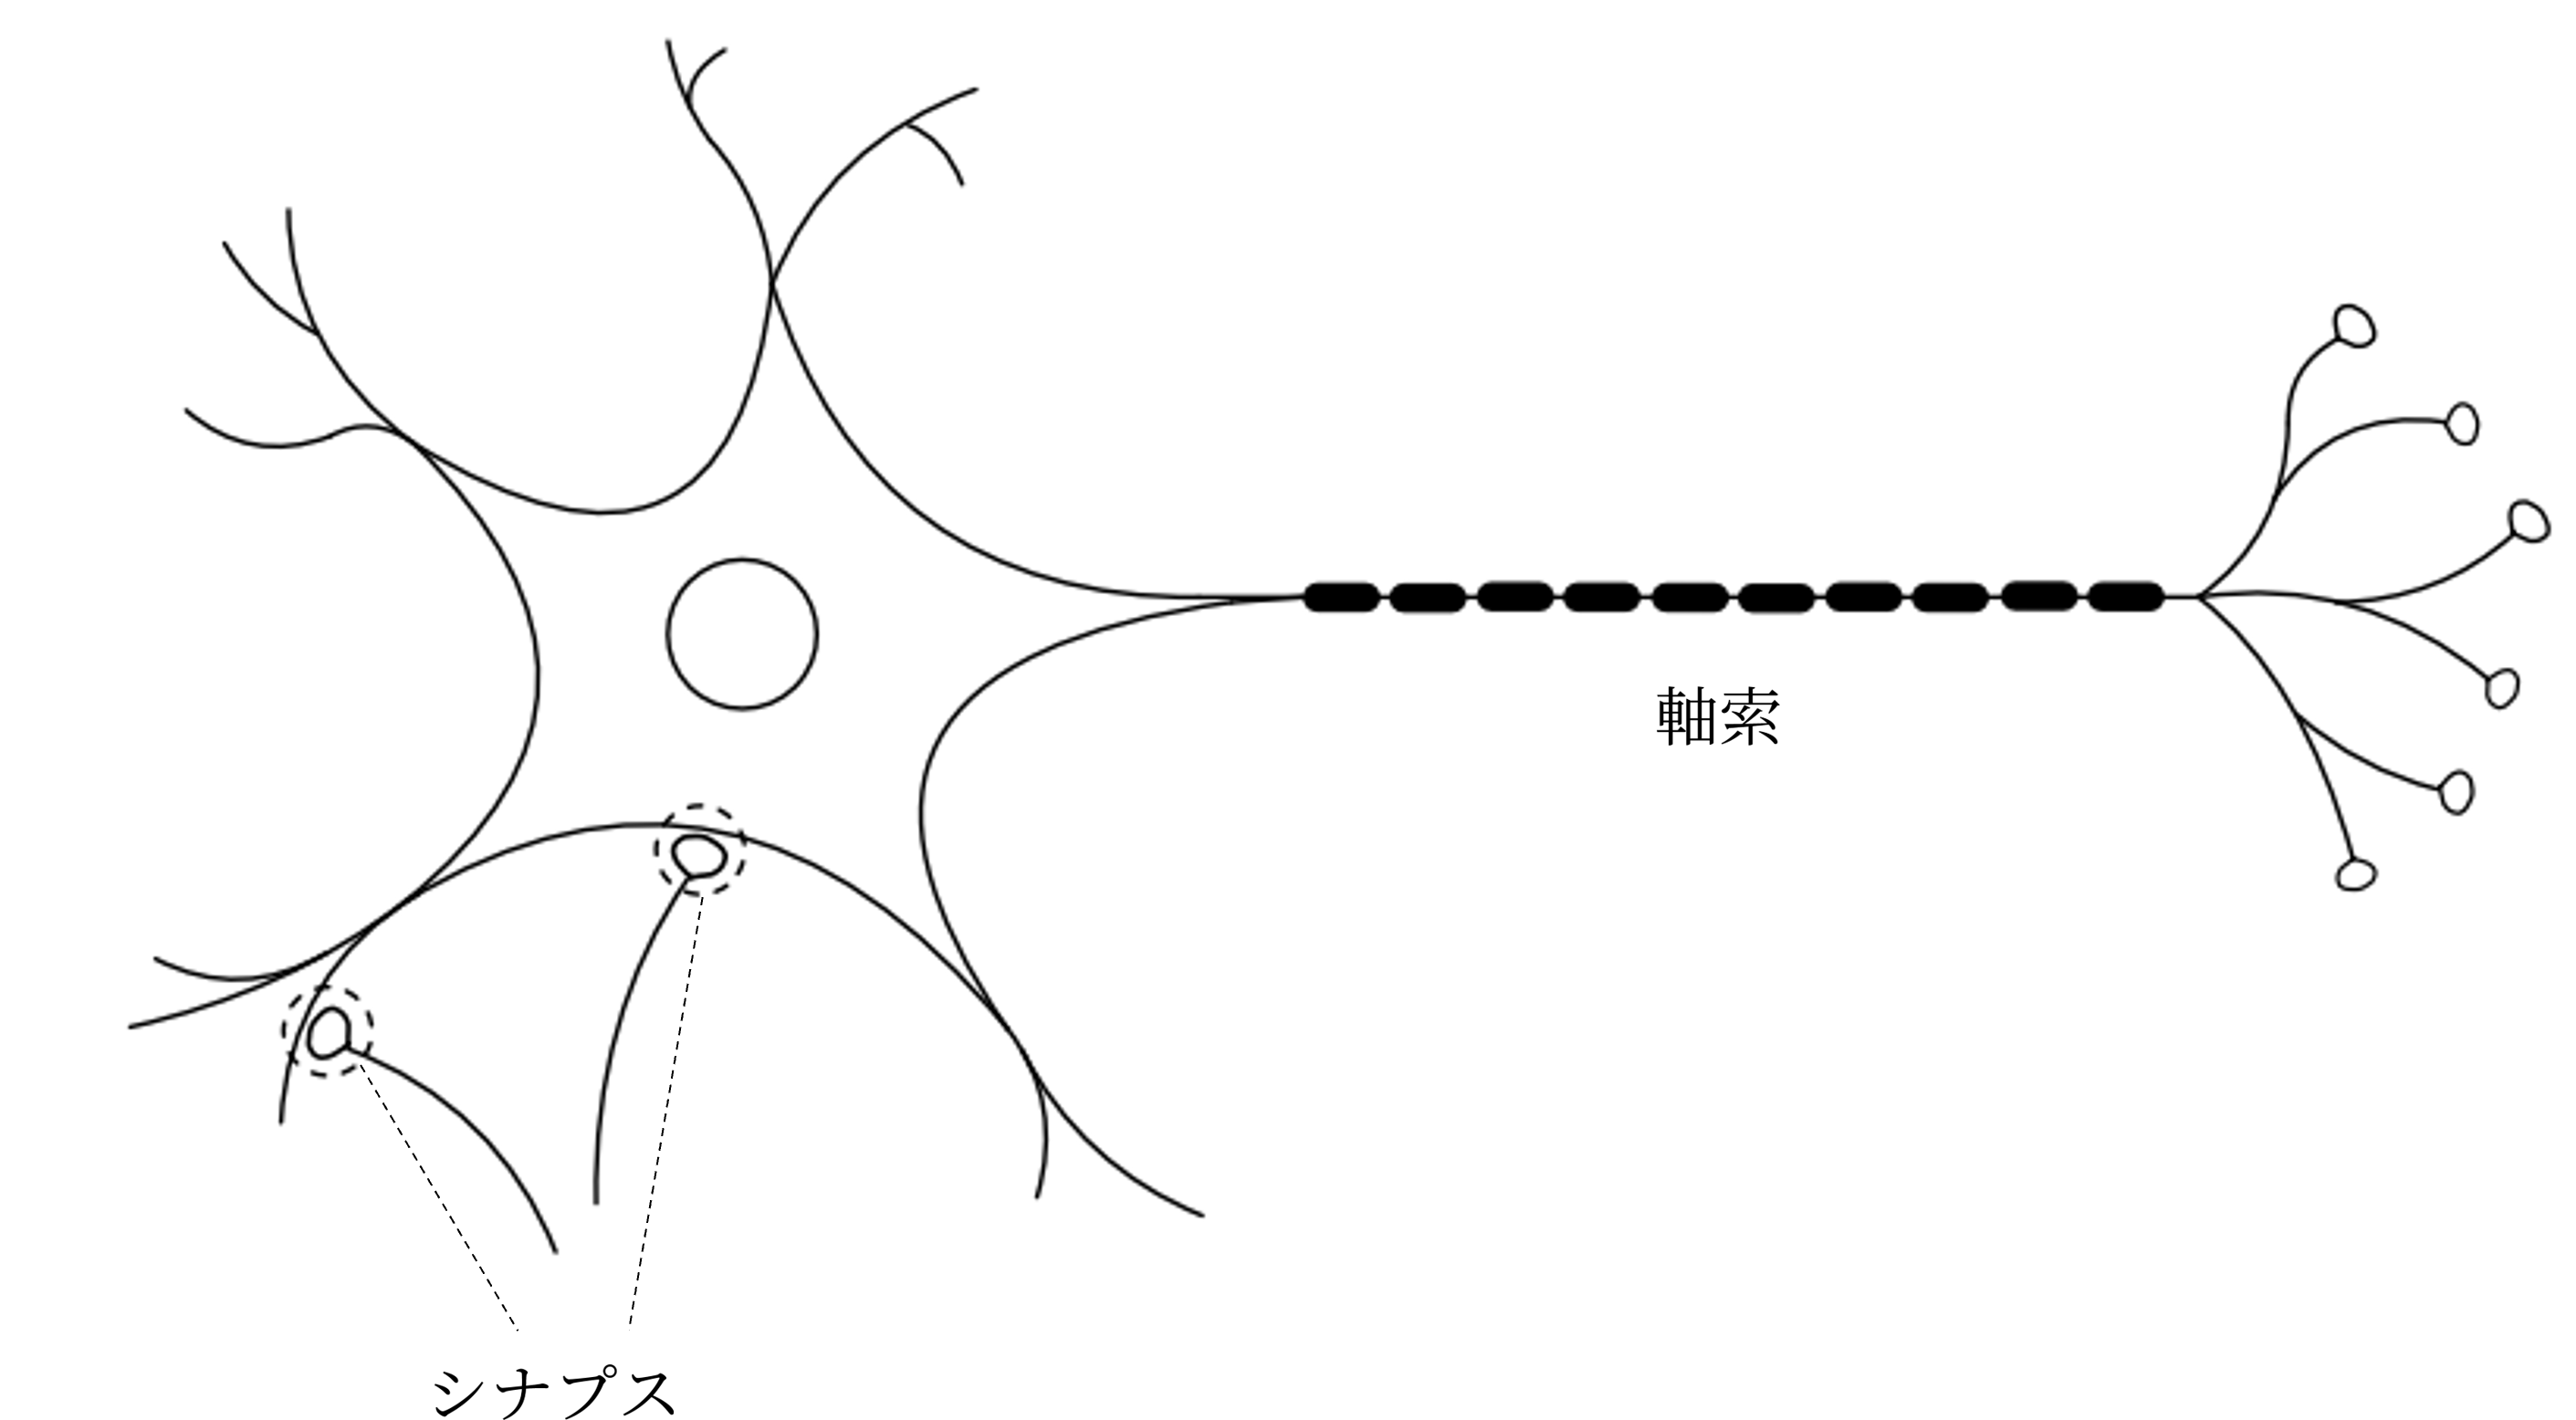
\includegraphics[height=7cm]{image/ニューロン.png}
    \subcaption{ニューロンの概要図}
    \label{ニューロン}
    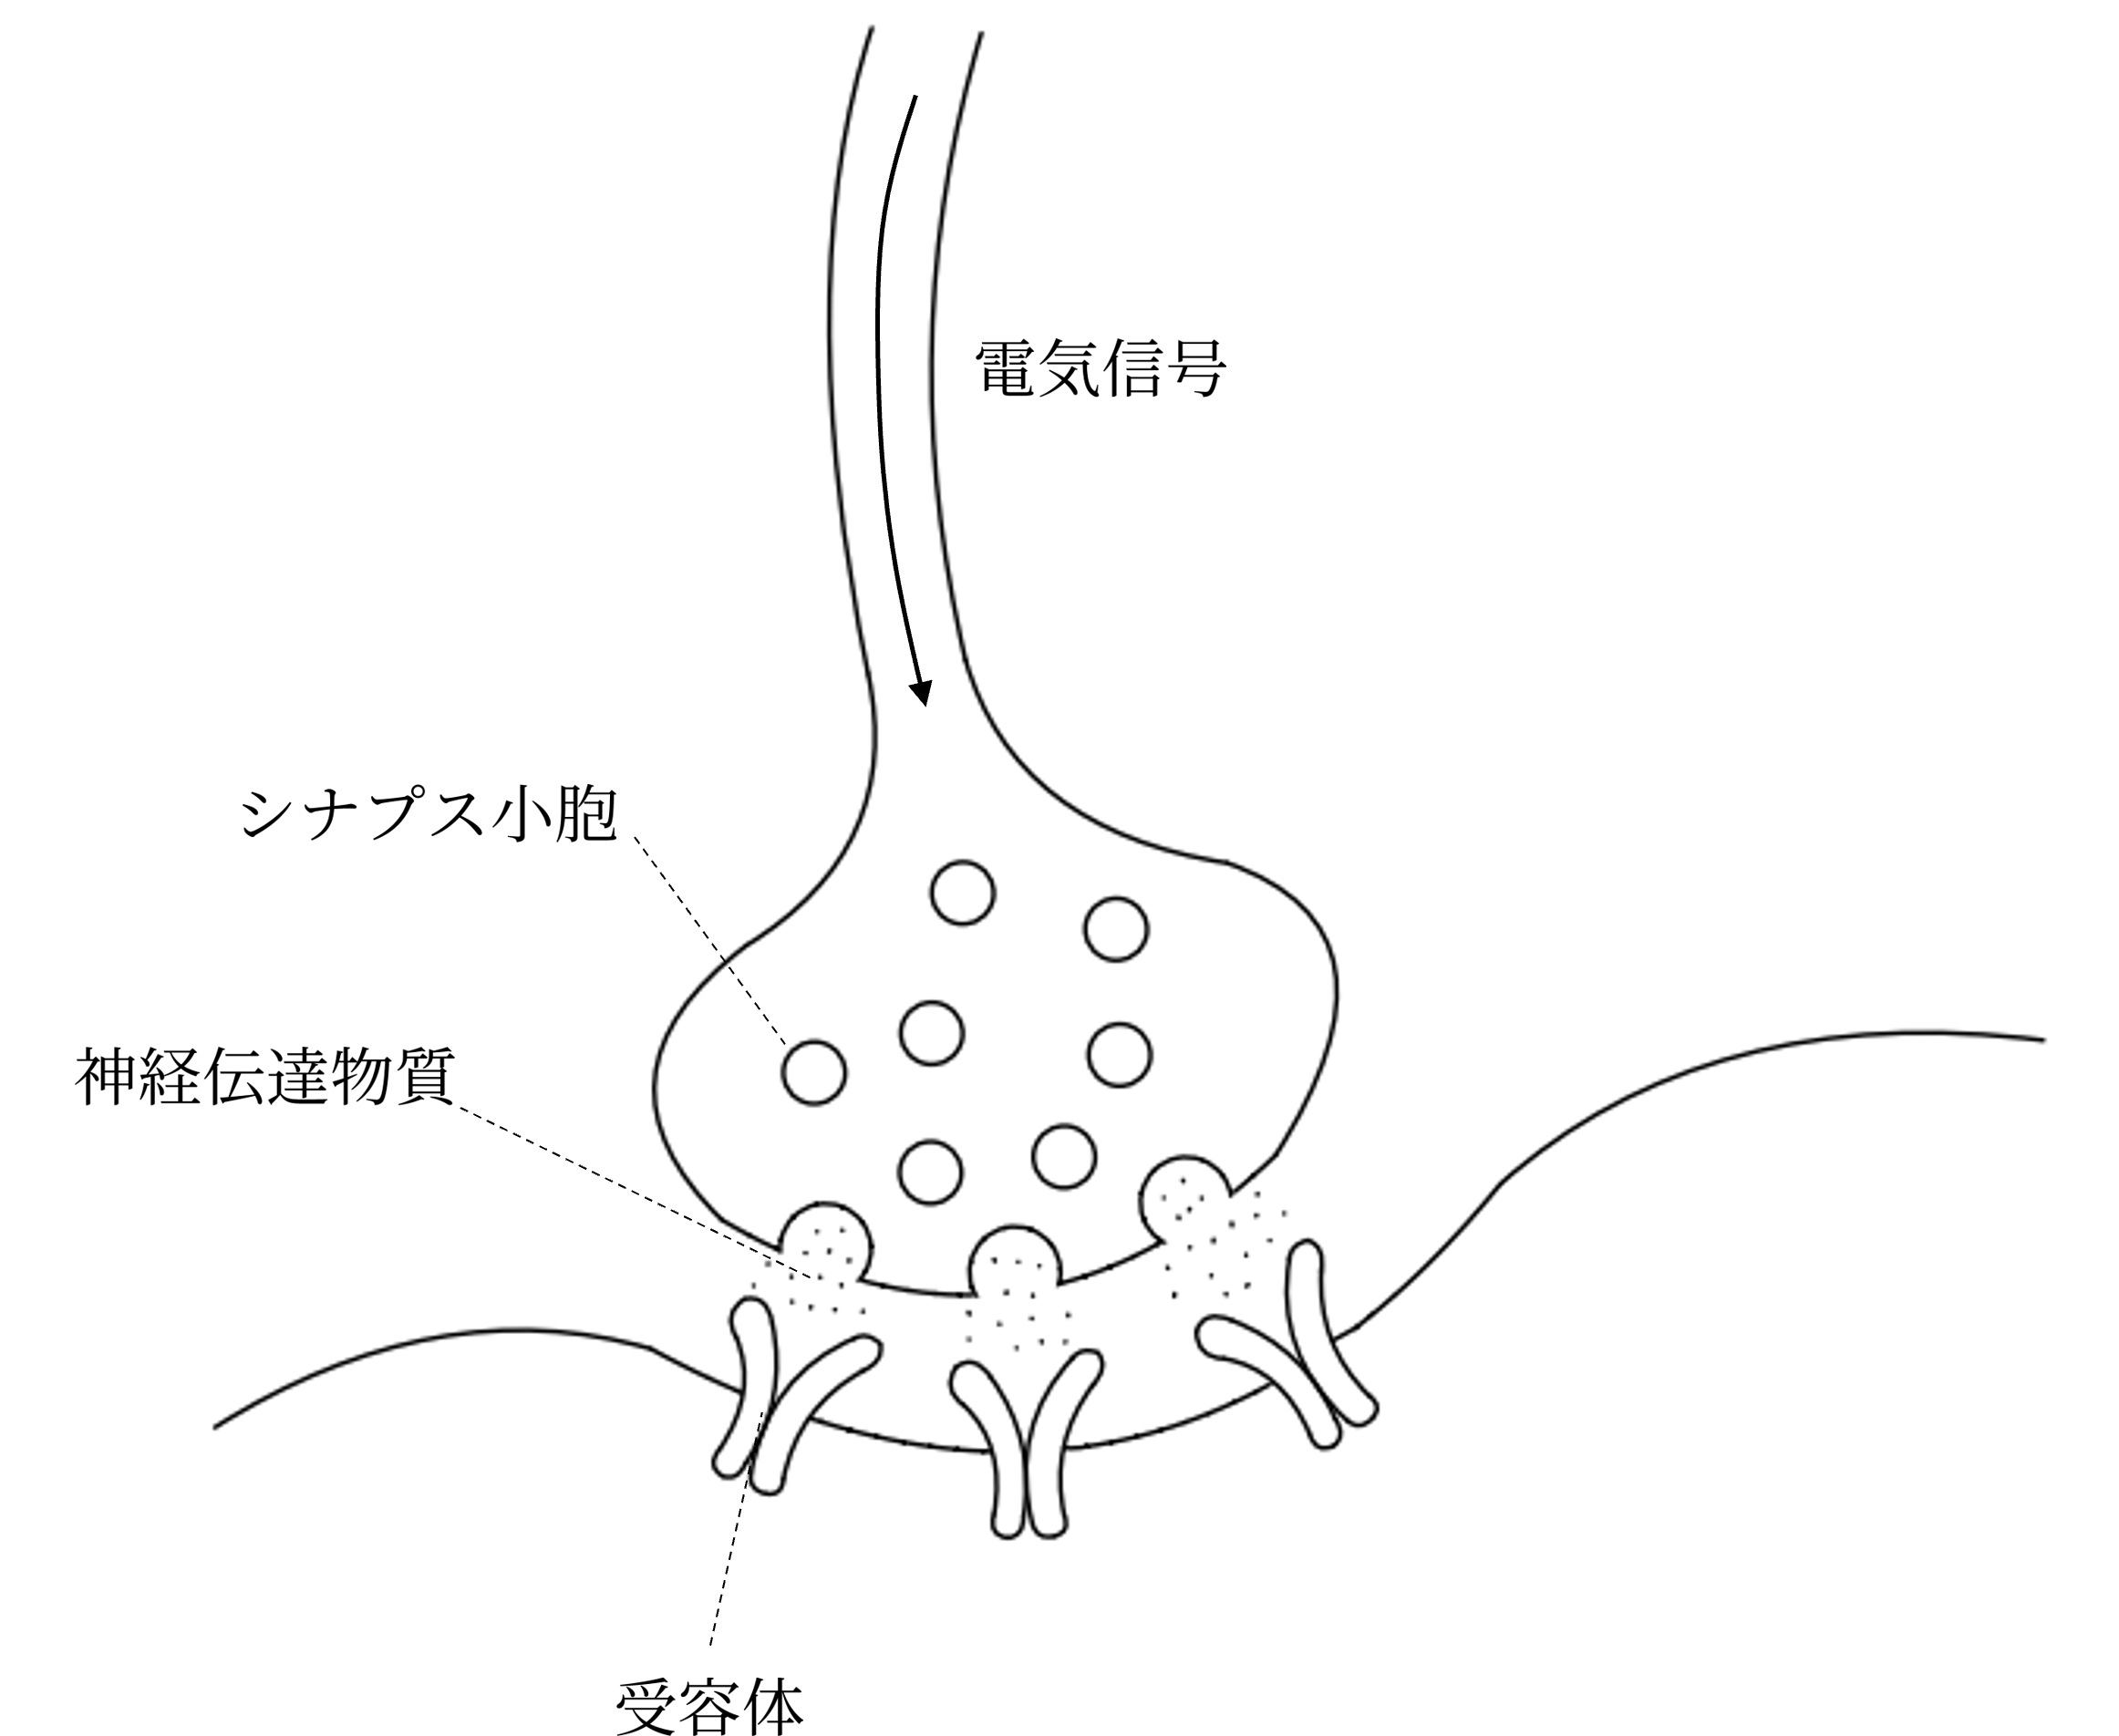
\includegraphics[height=6cm]{image/シナプス.png}
    \subcaption{シナプスの概要図}
    \label{シナプス}
  \end{center}
  \caption{ニューロンとシナプスの概要図}
\end{figure}
人間の脳は,1000億個以上ものニューロンと呼ばれる神経細胞が寄り集まって構成されている.ニューロンの形状は1873年にC.ゴルジが銀とクロムを用いた細胞の染色法によって観察に成功したことで明らかになった.図\ref{ニューロン}の形状を簡単に表した図である.ニューロンは通常の細胞とは大きく異なり,約10$\mathrm{\mu}$mほどの大きさの細胞体と呼ばれる部分から何本もの突起が伸びた構造をしている.このうち1本ある細長い突起は軸索と呼ばれ,その長さはヒトの場合,1mmから1mである.軸索の先端付近ではいくつもの分岐しており,これらを軸索側枝と呼ぶ.側枝はせいぜい数十$\mathrm{\mu}$mほどの長さしかない.そして側枝の終端を軸索終末と呼ぶ.軸索以外の突起は樹状突起と呼ばれる.樹状突起は植物の根のような途中でいくつも枝分かれした形状をしており,樹状突起の全長はせいぜい数mmと,軸索と比べるとはるかに短い.\par
このように突起がたくさん飛び出したニューロンがたくさん集まり,それらが規則的に接合を繰り返して脳はできている.図\ref{ニューロン}の丸で囲まれた部分がニューロン同士が接合する部分でこれをシナプスと呼ぶ.シナプスは軸索終末と樹状突起,または細胞体と接合して形成される.シナプスを拡大したものが図\ref{シナプス}である.\par
% では,軸索,樹状突起,そしてシナプスはどのような働きをしているかといいうと,まず軸索も樹状突起も,電気信号(パルス)を伝える電線のような役割を果たしている.神経回路上の電気信号は,極めて短い時間だけ立ち上がるパルスとして伝播する.このパルスの振幅は決まっているため,パルスの波の高さが信号の大きさを決めるわけではない.パルスは短い時間に細かく密集して伝わるが,信号強度に対応するのはそのパルスの密度である.\par
シナプス部ではまず,軸索に伝わってきた電気信号を合図に,軸索終末がシナプス小胞というカプセルに詰め込まれた化学物質を外にばらまく.その化学物質は神経伝達物質とよばれ,放出後はシナプスの樹状突起側で受け止められる.この場所には多数のレセプターがあり,そこに神経伝達物質が結合すると,その刺激から新たな電気信号が生み出される仕組みになっている.シナプスは樹状突起上にたくさんあり,各シナプスで樹状突起は他のさまざまなニューロンから電気信号の出力を受け入れる.この電気信号は細胞体へと向かって伝播する.そして数多くの樹状突起から伝わってきた電気信号は,細胞体に到達しすべて合算される.\par
細胞体は,ある一定以上の大きさ,つまり閾値を越える電気信号を受けると,軸索に向かって電気信号を出力する.電気信号は各軸索終末にあるシナプスにおいて他のニューロンの樹状突起に入力し,同じ伝播のパターンを繰り返していく.このように相互作用を複数に繰り返すことで,神経細胞のネットワークはできている.


\subsection{形式ニューロン}
\begin{figure}[H]
  \centering
  \begin{tikzpicture}[scale=1/2]
    \draw[-{Latex[length=2mm]}](1,0)--(8,0);
    \draw[-{Latex[length=2mm]}](-7,0)--(-1,0);
    \draw[-{Latex[length=2mm]}](-7,3.5)--(-0.84,0.55);
    \draw[-{Latex[length=2mm]}](-7,-3.5)--(-0.84,-0.55);
    \draw(0,1)--(0,-1);
    \draw (0,0) circle[radius=1];
    \draw (-0.5,0) node{$u$};
    \draw (0.5,0) node{$z$};
    \draw (-8,0) node{$x_2$};
    \draw (-8,4) node{$x_1$};
    \draw (-8,-4) node{$x_3$};
    \draw (-4,2.7) node{$w_1$};
    \draw (-4,0.5) node{$w_2$};
    \draw (-4,-3) node{$w_3$};
  \end{tikzpicture}
  \caption{形式ニューロンの例}
  \label{形式ニューロン}
\end{figure}
1943年にW.マカロックとW.ピッツによってニューロンの活動を数理論理学的な手法でモデル化できることを発見し,神経活動の数理モデルと論理回路との対応を明らかにした.彼らは,形式ニューロン,または人工ニューロンとよばれる素子を定義した.図\ref{形式ニューロン}はその一例である.実際のニューロンのように,形式ニューロンも他の多数の形式ニューロン$i=1,2,\dots$から入力信号$x_i$を受け入れる.図\ref{形式ニューロン}では入り込んでくる複数の矢印として入力を表している.ただし,ニューロンを出す信号はオンとオフの情報しかないとして,$x_i$の値は$0$か$1$しかとらないものとする.しかしシナプスごとに,ニューロン同士の結合の強さが違うため,重み$w_i$を導入して,層への総入力を
\begin{equation}
  u = \sum_{i} w_i x_i
\end{equation}
と定義する.$u$は細胞体に実際に入ってくる電気信号の総量に相当する.\par
総入力$u$を受けて,ニューロンは「軸索」方向へ出力を出すが,そこには閾値があるはずである.その状況をヘビサイドの階段関数
\begin{equation}
  \theta(x+b) = \begin{cases}
    1 & (x \geq -b) \\
    0 & (x \leq -b) \\
  \end{cases}
\end{equation}
でモデル化する.$b$は閾値を与えるパラメータである.すると,この形式ニューロンの出力は結局
\begin{equation}
  z = \theta(u + b) = \theta\left( \sum_{i} w_i x_i + b \right)
\end{equation}
となる.ここで用いた階段関数のように,総入力$u$を出力$z$へ変換する関数を一般的に活性化関数という.活性化関数に階段関数を用いため,$z$の値もまた,$0$か$1$の2値となり,それを再び他のニューロンへの入力とすることができる.\par
マカロックとピッツの形式ニューロンを多数組み合わせることで,計算機と同じようにどんな論理演算でも実現することができる.任意の論理回路がNANDゲートの組み合わせで実現できることは計算機科学でよく知られているため,この証明はNANDゲートの出力を実現する形式ニューロンの回路を組めることを示せばよい.\par
NANDゲートとは,2つの2値入力$x_1, x_2$に対する出力値の関係が次のようになっている論理回路のことである.
\begin{equation*}
  \begin{tabular}{c|cccc}
    $(x_1, x_2)$ & $(0,0)$ & $(1,0)$ & $(0,1)$ & $(1,1)$ \\ \hline
    $y$          & $1$     & $1$     & $1$     & $0$     \\
  \end{tabular}
\end{equation*}
つまり,2つの入力$x_1, x_2$からなる形式ニューロン(図\ref{ニューロン回路の例})を考え,NANDゲートによる出力$y$を満たすような重みとバイアスの値を見つければよいということである.\par
\begin{figure}[H]
  \centering
    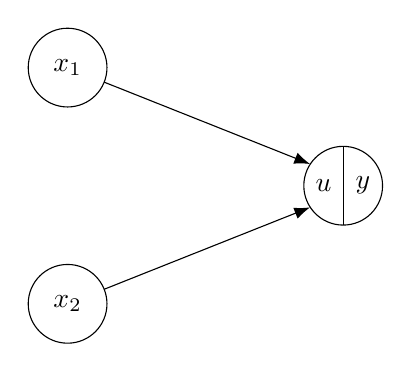
\begin{tikzpicture}[scale=1/2]
      \draw[-{Latex[length=2mm]}](-7,3)--(-0.84,0.55);
      \draw[-{Latex[length=2mm]}](-7,-3)--(-0.84,-0.55);
      \filldraw[fill=white] (0,0) circle[radius=1];
      \filldraw[fill=white] (-7,3) circle[radius=1];
      \filldraw[fill=white] (-7,-3) circle[radius=1];
      \draw(0,1)--(0,-1);
      \draw (-0.5,0) node{$u$};
      \draw (0.5,0) node{$y$};
      \draw (-7,3) node{$x_1$};
      \draw (-7,-3) node{$x_2$};
    \end{tikzpicture}
    \caption{簡単なニューロン回路の例}
    \label{ニューロン回路の例}
\end{figure}
これは簡単に見つけることができ,例えば
\begin{align}
  y
  &= \theta(w_1 x_1 + w_2 x_2 + b) \notag \\
  &= \theta(-x_1 - x_2 + 1.5)
\end{align}
とすればよい.実際
\begin{align*}
  y(0,0) & = \theta(1.5) = 1  \\
  y(1,0) & = \theta(0.5) = 1  \\
  y(0,1) & = \theta(0.5) = 1  \\
  y(1,1) & = \theta(-0.5) = 0 \\
\end{align*}
となり,NANDゲートの出力そのものであると分かる.したがって,このニューロン回路を適切に組み合わせることにより,任意の論理演算を実現することができる.

\subsection{パーセプトロン}
\begin{figure}[H]
  \begin{center}
    \centering
    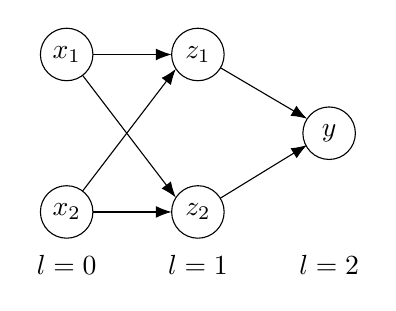
\begin{tikzpicture}[scale=1/3]
      \draw[-{Latex[length=2mm]}](-5,3)--(-0.84,-2.45);
      \draw[-{Latex[length=2mm]}](-5,-3)--(-0.84,2.45);
      \draw[-{Latex[length=2mm]}](0,3)--(4.16,0.55);
      \draw[-{Latex[length=2mm]}](0,-3)--(4.16,-0.45);
      \draw[-{Latex[length=2mm]}](-5,3)--(-1,3);
      \draw[-{Latex[length=2mm]}](-5,-3)--(-1,-3);
      \filldraw[fill=white] (0,3) circle[radius=1];
      \filldraw[fill=white] (0,-3) circle[radius=1];
      \filldraw[fill=white] (-5,3) circle[radius=1];
      \filldraw[fill=white] (-5,-3) circle[radius=1];
      \filldraw[fill=white] (5,0) circle[radius=1];
      \draw (0,3) node{$z_1$};
      \draw (0,-3) node{$z_2$};
      \draw (-5,3) node{$x_1$};
      \draw (-5,-3) node{$x_2$};
      \draw (5,0) node{$y$};
      \draw (-5,-5) node{$l=0$};
      \draw (0,-5) node{$l=1$};
      \draw (5,-5) node{$l=2$};
    \end{tikzpicture}
    \caption{2層のパーセプトロン}
    \label{2層パーセプトロン}
  \end{center}
\end{figure}
形式ニューロンでどんな論理回路でも作ることがわかったが,解きたい問題をニューロン回路によって計算してくれる効率的な回路が設計できるがはわからない.そこでローゼンブラットは形式ニューロンのネットワークの重み$w$とバイアス$b$を解きたい問題に対してよく処理できるように訓練させるという「教師あり学習」のアイデアを付け加えた.ここでは,パーセプトロンの構造について説明し,教師あり学習については3.9章で説明する.\par
パーセプトロンとは形式ニューロンを層構造をなすように複数組み合わせて作ったニューロン回路のことである.図\ref{2層パーセプトロン}はパーセプトロンの例で,$l=0,1,2$の3つの層で形成されている.最も左側にある層はデータが入力される部分であるため,入力層とよばれる.それに対して最も右側にある層は最終的な出力を行う層であることから,出力層とよばれる.そして,入力層と出力層の間にある層は中間層または隠れ層とよばれる.パーセプトロンでは層数に入力層を含めないため,これは2層のパーセプトロンである.\par
パーセプトロンで解きたい問題を解かせたい場合,各層で形式ニューロンの数をいくつに設定すればよいかというと,入力層は入力値のベクトル$\bm{x}^{\top}=(x_1, x_2, \cdots)$の各成分$x_i$を出力値としてもつ入力用の形式ニューロンの集まりであるため,入力ベクトルの次元の数に,出力層は推定したい最終結果$\bm{t}^{\top}=(y_1, y_2, \cdots)$の各成分$y_i$の数で設定する必要がある.中間層の形式ニューロン数に関しては特に制限はない.さらに,中間層は層数を2つ以上に設定してもよい.

\subsection{順伝播ニューラルネットワーク}
これまでの形式ニューロンやパーセプトロンについて説明した.ここでは,それらをもとにした現代の順伝播ニューラルネットワークについて説明する.\par
\begin{figure}[H]
  \centering
  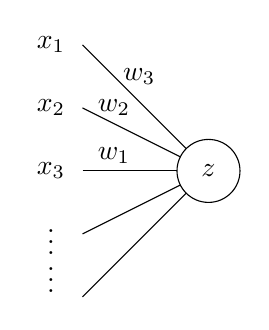
\begin{tikzpicture}[scale=1/2.5]
    \draw (-4,4)--(0,0);
    \draw (-4,2)--(0,0);
    \draw (-4,0)--(0,0);
    \draw (-4,-2)--(0,0);
    \draw (-4,-4)--(0,0);
    \filldraw[fill=white] (0,0) circle[radius=1];
    \draw (-5,4) node{$x_1$};
    \draw (-5,2) node{$x_2$};
    \draw (-5,0) node{$x_3$};
    \draw (-3,0.5) node{$w_1$};
    \draw (-3,2) node{$w_2$};
    \draw (-2.2,3) node{$w_3$};
    \draw (0,0) node{$z$};
    \draw (-5,-2) node{$\vdots$};
    \draw (-5,-3.2) node{$\vdots$};
  \end{tikzpicture}
  \caption{ユニットの構造.$x_1,x_2,\dots$の入力を受け,$z$を出力する}
  \label{ユニットの構造}
\end{figure}
順伝播型ニューラルネットワークでは丸で書かれた素子のことをユニット,ユニット間を結ぶ線のことをエッジとよぶ.図\ref{ユニットの構造}はユニットの構造を示したものである.見た目はパーセプトロンにおける形式ニューロンと変わらない.しかし,ユニットは形式ニューロンとは違い,0,1の値ではなく,実数値の入出力を持つことができる.また,もう1つの大きな違いは,活性化関数として階段関数ではなく,微分可能は増化関数を採用するということである.まず,ユニットにさまざまな入力$x_i$は入ってきているとする.各ユニットによって結合強度が異なるため,実際にはそれらの重み付き和
\begin{equation}
  u = \sum_{i} w_i x_i
\end{equation}
がユニットへの総入力となる.$u$は活性とも呼ばれる.この活性にバイアス$b$を加えたうえで,さらに活性化関数$f$での変換を施したものが,このユニットからの出力$z$になる.
\begin{equation}
  z = f(u + b) = f\left( \sum_{i} w_i x_i + b \right)
\end{equation}
活性化関数は閾値$-b$を超えるとニューロンが信号を発することをモデル化する部分であるため,昔の研究では階段関数によく似た連続関数がよく用いられていた.その一例がシグモイド関数
\begin{equation}
  \sigma(u + b) = \frac{1}{1 + e^{-u-b}}
\end{equation}
である.図\ref{シグモイド関数}をみると,閾値付近で信号が立ち上がっていることがわかる.
\begin{figure}[H]
  \begin{center}
    \centering
    \begin{tikzpicture}[scale=2,samples=300]
      \draw[->,>=stealth,semithick](-2,0)--(2,0)node[below]{$u$};%x軸
      \draw[->,>=stealth,semithick](0,-0.5)--(0,1.5)node[above]{$\sigma(u+b)$};%y軸
      \draw (-0.5,0.08)--(-0.5,-0.08)node[below]{-b};
      \draw (0.08,1)--(-0.08,1)node[left]{1};
      \draw (0,0)node[below left]{0};
      \draw[draw=magenta,thick,domain=-2:2] plot(\x,{1/(1+pow(e,-6*\x-3))});
    \end{tikzpicture}
    \caption{シグモイド関数}
    \label{シグモイド関数}
  \end{center}
\end{figure}

順伝播型ニューラルネットワークとはこのようなユニットを層状につなぎ合わせたアーキテクチャである.図\ref{順伝播ニューラルネットワークの例}はその典型的な一例である\footnote{本論文ではニューラルネットワークのユニット同士をつなぐ線を矢印ではなく,線で表すことにする.}.$l$は層数で,$l=0$が入力層,$l=3$が出力層,そして,$l=1,2$が中間層を表している.信号の伝達は$l=0,1,2,3$の順に進み,そのため順伝播型と呼ばれる.\par

\begin{figure}[H]
  \begin{center}
    \centering
    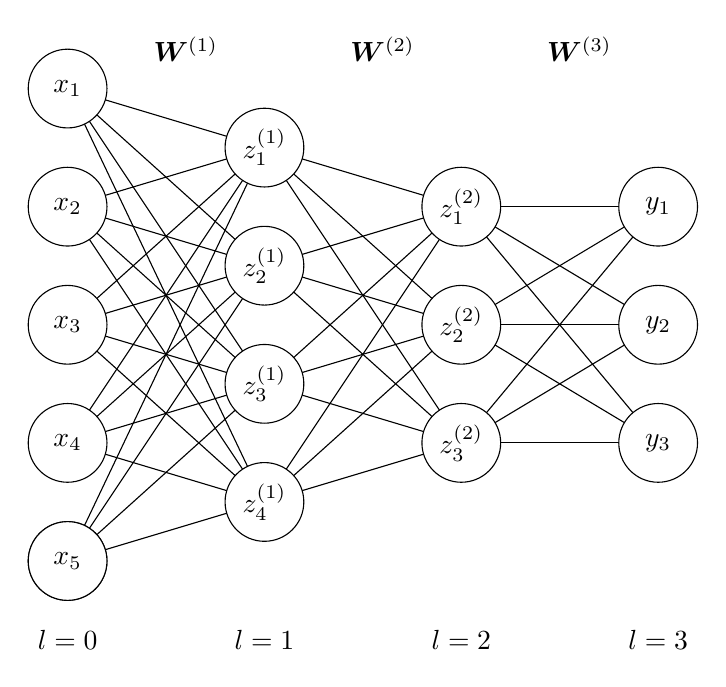
\begin{tikzpicture}[scale=1/2]
      \draw (0,0)--(5,1.5);
      \draw (0,0)--(5,4.5);
      \draw (0,0)--(5,7.5);
      \draw (0,0)--(5,10.5);
      \draw (0,3)--(5,1.5);
      \draw (0,3)--(5,4.5);
      \draw (0,3)--(5,7.5);
      \draw (0,3)--(5,10.5);
      \draw (0,6)--(5,1.5);
      \draw (0,6)--(5,4.5);
      \draw (0,6)--(5,7.5);
      \draw (0,6)--(5,10.5);
      \draw (0,9)--(5,1.5);
      \draw (0,9)--(5,4.5);
      \draw (0,9)--(5,7.5);
      \draw (0,9)--(5,10.5);
      \draw (0,12)--(5,1.5);
      \draw (0,12)--(5,4.5);
      \draw (0,12)--(5,7.5);
      \draw (0,12)--(5,10.5);
      \draw (5,1.5)--(10,3);
      \draw (5,1.5)--(10,6);
      \draw (5,1.5)--(10,9);
      \draw (5,4.5)--(10,3);
      \draw (5,4.5)--(10,6);
      \draw (5,4.5)--(10,9);
      \draw (5,7.5)--(10,3);
      \draw (5,7.5)--(10,6);
      \draw (5,7.5)--(10,9);
      \draw (5,10.5)--(10,3);
      \draw (5,10.5)--(10,6);
      \draw (5,10.5)--(10,9);
      \draw (10,3)--(15,3);
      \draw (10,3)--(15,6);
      \draw (10,3)--(15,9);
      \draw (10,6)--(15,3);
      \draw (10,6)--(15,6);
      \draw (10,6)--(15,9);
      \draw (10,9)--(15,3);
      \draw (10,9)--(15,6);
      \draw (10,9)--(15,9);
      \filldraw[fill=white] (0,0) circle[radius=1];
      \filldraw[fill=white] (0,3) circle[radius=1];
      \filldraw[fill=white] (0,6) circle[radius=1];
      \filldraw[fill=white] (0,9) circle[radius=1];
      \filldraw[fill=white] (0,12) circle[radius=1];
      \filldraw[fill=white] (5,1.5) circle[radius=1];
      \filldraw[fill=white] (5,4.5) circle[radius=1];
      \filldraw[fill=white] (5,7.5) circle[radius=1];
      \filldraw[fill=white] (5,10.5) circle[radius=1];
      \filldraw[fill=white] (10,3) circle[radius=1];
      \filldraw[fill=white] (10,6) circle[radius=1];
      \filldraw[fill=white] (10,9) circle[radius=1];
      \filldraw[fill=white] (15,3) circle[radius=1];
      \filldraw[fill=white] (15,6) circle[radius=1];
      \filldraw[fill=white] (15,9) circle[radius=1];
      \filldraw[fill=white] (0,0) circle[radius=1];
      \draw (0,0) node{$x_5$};
      \draw (0,3) node{$x_4$};
      \draw (0,6) node{$x_3$};
      \draw (0,9) node{$x_2$};
      \draw (0,12) node{$x_1$};
      \draw (3,13) node{$\bm{W}^{(1)}$};
      \draw (8,13) node{$\bm{W}^{(2)}$};
      \draw (13,13) node{$\bm{W}^{(3)}$};
      \draw (5,1.5) node{$z_4^{(1)}$};
      \draw (5,4.5) node{$z_3^{(1)}$};
      \draw (5,7.5) node{$z_2^{(1)}$};
      \draw (5,10.5) node{$z_1^{(1)}$};
      \draw (10,3) node{$z_3^{(2)}$};
      \draw (10,6) node{$z_2^{(2)}$};
      \draw (10,9) node{$z_1^{(2)}$};
      \draw (15,3) node{$y_3$};
      \draw (15,6) node{$y_2$};
      \draw (15,9) node{$y_1$};
      \draw (0,-2) node{$l=0$};
      \draw (5,-2) node{$l=1$};
      \draw (10,-2) node{$l=2$};
      \draw (15,-2) node{$l=3$};
    \end{tikzpicture}
    \caption{入力層と3層からなる順伝播ニューラルネットワークの例.ユニットを表す丸の中に書かれた変数は,各ユニットの出力値を意味する.}
    \label{順伝播ニューラルネットワークの例}
  \end{center}
\end{figure}

一般的な順伝播型ニューラルネットワークを考える.まず,入力層の各ユニットはニューラルネットワーク全体への入力ベクトル$\bm{x}^{\top}=(x_1, x_2, \cdots)$の各成分が入力して,それをそのまま出力する.つまり,入力ユニットは活性化関数をもたず,単に値$x_i$を出力するだけである.入力層は入力ベクトル$\bm{x}$の次元数だけユニットをもつ.また,「第0層からの出力である」という意味を込めて次のようなラベル付けをする.
\begin{equation}
  \bm{z}^{(0)} = \bm{x}
\end{equation}\par
次に中間層について考える.第$l$層中の$j$番目のユニットを考える.このユニットは第$l-1$層の各ユニットからの入力$z_i^{(l-1)}$を入力として受けるため.活性は
\begin{equation}
  u_l^{(l)} = \sum_i w_{ji}^{(l)} z_i^{(l-1)}
\end{equation}
となる.ただし$w_{ji}^{(l)}$は,第$l-1$層のユニット$i$を第$l$層のユニット$j$の間の結合の重みである.\par
ユニットの出力は,活性$u_j^{(l)}$にユニット固有のバイアス$b_j^{(l)}$を加え,さらに活性化関数$f^{(l)}$を作用させたもの
\begin{equation}
  z_j^{(l)}
  = f^{(l)} \left( u_j^{(l)} + b_j^{(l)} \right)
  = f^{(l)} \left( \sum_i w_{ji}^{(l)} z_i^{(l-1)} + b_j^{(l)} \right)
\end{equation}
で与えられる.\footnote{活性化関数は$f^{(l)}$はユニットごとに変えても問題ないが,一般的には層ごとに共通の関数を用いる.}\par
これらの式を行列表示しよう.まず$l$層の全ユニットの活性をまとめてベクトル$\bm{u}^{(l)}=\left( u_j^{(l)} \right)$で,出力をまとめて$\bm{z}^{(l)}=\left( z_j^{(l)} \right)$で表す.また,第$l-1$層のユニット$i$と第$l$層のユニット$j$の間の結合の重み$w_{ji}^{(l)}$を$(j,i)$成分とする重み行列
\begin{equation}
  \bm{W}^{(l)}
  =\begin{pmatrix}
    w_{11}^{(l)} & w_{11}^{(l)} & \cdots \\
    w_{21}^{(l)} & w_{22}^{(l)} &        \\
    \vdots       &              & \ddots \\
  \end{pmatrix}
\end{equation}
も導入する.さらにバイアスのまとめて縦ベクトル$\bm{b}^{(l)} = \left( b_j^{(l)} \right)$で表記することにすると,中間層が行う演算処理は
\begin{equation}
  \bm{u}^{(l)}
  = \bm{W}^{(l)} \bm{z}^{(l-1)}, \ \ \ \bm{z}^{(l)} = f^{(l)}\left( \bm{u}^{(l)} + \bm{b}^{(l)} \right)
\end{equation}
とまとめることができる.ただし,一般のベクトル$\bm{v}^{\top} = \begin{pmatrix} v_1 & v_2 & v_3 & \cdots \end{pmatrix}$に対する関数$f$の作用は,次のように各成分にそれぞれ作用するものとして定義することにする.\par
\begin{equation}
  f(\bm{v}) = f\begin{pmatrix}
    v_1 \\ v_2 \\ v_3 \\ \vdots
  \end{pmatrix} = \begin{pmatrix}
    (f(\bm{v}))_1 \\ (f(\bm{v}))_2 \\ (f(\bm{v}))_3 \\ \vdots
  \end{pmatrix} \equiv \begin{pmatrix}
    f(v_1) \\ f(v_2) \\ f(v_3) \\ \vdots
  \end{pmatrix}
\end{equation}
これまで重みとバイアスを区別して書いたが,バイアスも重みに含めてしまうことができる.それを理解するためにすべての中間層(と入力層)に,常に$1$という出力をするユニットを1つ加える.そしてそれを$i=0$というラベルで呼ぶことにする.
\begin{equation}
  z_0^{(l)} = 1
\end{equation}\par
第$l-1$層の$i=0$と第$l$層の$j \neq 0$の間に重み$w_{j0}^{l}$を導入する.すると,これはバイアスそのものになる.なぜなら$w_{j0}^l = b_j^l$とおくと,
\begin{equation}
  \sum_{i=0} w_{ji}^l z_i^{l-1}
  = \sum_{i=1} w_{ji}^l z_i^{l-1} + w_{j0}^l
  = \sum_{i=1} w_{ji}^l z_i^{l-1} + b_j^l
\end{equation}
となるからである.そのため,今後,必要のない場合は重みの中にバイアスも含めてしまい,バイアスをあらわに書かない次のような表記を用いることにする.
\begin{equation}
  \bm{u}^{(l)}
  = \bm{W}^{(l)} \bm{z}^{(l-1)}, \ \ \ \bm{z}^{(l)} = f^{(l)}\left( \bm{u}^{(l)} \right)
\end{equation}\par
最後に出力層について考える.$L$層からなる順伝播型ニューラルネットワークを考える.すると最後の第$L$層が出力層に相当する.出力層は,手前の第$L-1$層から$\bm{z}^{(L-1)}$を入力され,それを変換することでニューラルネットの最終出力$\bm{y}=\bm{z}^{L}$を出力する.出力層の役割は,回帰など機械学習で実行したいタスクを処理することである.つまり,$\bm{h}=\bm{z}^{(L-1)}$が入力$\bm{x}$の表現であり,この表現$\bm{h}$の回帰分析を通じて$\bm{x}$と$\bm{y}$の関係を推定するのが出力層の役割である.\par
\begin{equation}
  \hat{\bm{y}}
  = \bm{z}^{(L)}
  = f^{(L)}\left( \bm{u}^{(L)} \right), \ \ \
  \bm{u}^{(L)}
  = \bm{W}^{(L)} \bm{h}
\end{equation}
出力層においては,活性化関数の値域が目標変数の値域と一致するように$f^{(L)}$を選ぶ必要がある.\par
入力層から出力層に至る一連の情報処理の仕組みを説明した.結局のところ順伝播型ニューラルネットは,各総出の処理を順次入力ベクトル$\bm{x}$に施していくことで,$\bm{x}$から次の出力値を与える関数モデルということになる.
\begin{equation}
  \hat{\bm{y}}
  = f^{(L)}\left( \bm{W}^{(L)}f^{(L-1)} \left( \bm{W}^{(L-1)}f^{(L-2)} \left( \cdots \bm{W}^{(2)}f^{(1)}(\bm{x}) \right) \right) \right)
\end{equation}

\section{ニューラルネットワークによる機械あり学習}
これまで,脳の神経回路を模した数理モデルとしてニューラルネットワークを定義した.ここでは,構築したニューラルネットワークに対して,機械学習によってタスクを遂行させるにはどうすればよいかを説明する.\par
順伝播ニューラルネットは入力$\bm{x}$を受け取ることで出力
\begin{equation}
  \bm{y}(\bm{x}; \bm{w})
  \equiv \bm{y}\left( \bm{x}; \bm{W}^{(1)},\dots ,\bm{W}^{(L)},\bm{b}^{(1)},\dots ,\bm{b}^{(L)} \right) \label{NN出力}
\end{equation}
を出す.ただし,重み$\bm{W}^{(l)}$とバイアス$\bm{b}^{(l)}$をまとめて$\bm{w}$と書いた.したがって,出力の値はパラメータ$\bm{w}$によって決まることになる.この出力を機械学習における識別関数とみなすと,データを用いてパラメータ$\bm{w}$に関してフィッティングすることができる.この手順は通常の教師あり学習と同じであり,まず訓練データ$\mathcal{D}=\{ (\bm{x}_n, \bm{y}_n) \}_{n=1,\dots ,N}$を用意する.そのうえで訓練データ$\bm{x}_n$を入れた際のニューラルネットワークの出力値$\bm{y}(\bm{x}_n; \bm{w})$と,目標値$\bm{y}_n$のズレができるだけ小さくなるように,重みとバイアスを調整して学習する.ズレを測る誤差関数$E(\bm{w})$の選び方は,考えるタスクと出力層の構造に依存する.そして誤差関数の最小化
\begin{equation}
  \bm{w}^* = \underset{\bm{w}} {\operatorname{argmin}} \ E(\bm{w})
\end{equation}
が学習に対応する\par
式(\ref{NN出力})のように考えると,入力から一気に$\bm{y}$が得られているように見えるが,実際は層状の構造に従って信号が処理されていた.特に,第$L-1$層までの情報処理と,最後の出力層を切り分けて考えてみよう.なぜなら,第$L-1$層の部分までは,入力$\bm{x}$から層ごとに順次高次な表現を構成する役割を果たしているとみなせるからである.すると第$L-1$層からの出力は,入力$\bm{x}$に対する深層表現$\bm{h}$である.
\begin{equation}
  \bm{h}\left( \bm{x}; \bm{W}^{(1)},\dots ,\bm{W}^{(L-1)} \right)
  = \bm{z}^{(L-1)}\left( \bm{x}; \bm{W}^{(1)},\dots ,\bm{W}^{(L-1)} \right)
\end{equation}
すると出力層は,この表現を使って回帰のような通常の機械学習を行う役割を担っているとみなせる.\par
では次に,ニューラルネットワークにさせたいタスクごとに分けて,出力層の構造を見ていく.
\subsubsection*{回帰の場合}
もし表現$\bm{h}$について線形回帰を行いたいのであれば,自明な活性化関数,つまり単なる恒等写像を用いた出力層を用意すればよい.
\begin{equation}
  \bm{y}
  = \bm{W}^{(L)} \bm{h}
\end{equation}
このようなユニットは線形ユニットと呼ばれる.ただし多くの場合は線形ではない一般的な回帰を行いたいため,何らかの非自明な活性化関数を考える.
\begin{equation}
  \bm{y}(\bm{x}; \bm{\theta})
  = f^{(L)}\left( \bm{W}^{(L)} \bm{h} \right)
\end{equation}
具体的にどのような$f^{(L)}$を選ぶかは,問題の性質に応じて我々が設定する必要がある.\par
出力をデータでフィッティングするには,$\bm{y}(\bm{x}; \bm{\theta})$を用いたモデルの予測値と実際のデータができるだけ近くなるように,平均二乗誤差を最小化する.
\begin{equation}
  E(\bm{\theta})
  = \frac{1}{2} \sum_{n=1}^N \left( \bm{y}(\bm{x}_n; \bm{\theta}) - \bm{y}_n \right)^2, \ \ \
  \bm{\theta}^* = \underset{\bm{\theta}} {\operatorname{argmin}} \ E(\bm{\theta})
\end{equation}
学習により得られた最適パラメータ$\bm{\theta}^*$を代入したモデル$\bm{y}(\bm{x}; \bm{\theta}^*)$は,入力$\bm{x}$の値に応じて$\bm{y}$をよく予測できるようになるだろう.これが通常の回帰と異なるのは,回帰関数のパラメータだけでなく,表現を決める中間層の重みパラメータも同時に学習しているということである.これがニューラルネットワークによる表現学習である.

\subsubsection*{2値分類の場合}
回帰と並んで代表的なタスクは,データを2つのクラスに分類する2値分類であった.ただし,2つのクラスに対応するラベル$y$の値は0か1の2値であるとする.ニューラルネットワークで2値分類を表現するには,出力層が表現$\bm{h} = \bm{z}^{(L-1)}$のロジスティック回帰を与えるようにデザインすればよい.\par
訓練データ$\mathcal{D} = \{ (\bm{x}_n, y_n) \}_{n=1,\dots ,N}$の標準値$y_n$は0か1だが,ロジスティック回帰では,この2値変数そのものではなく,$y$が1である確率$\hat{y} = P(y=1 | \bm{x})$を推定する.言い換えれば$y$の期待値を推定する.なぜなら,2値変数$\mathrm{y}$の従うベルヌーイ分布のもとで期待値は$E_{P(y | \bm{x})}[\mathrm{y} | \bm{x}] = \sum_{y=0,1} y P(y | \bm{x}) = P(y=1 | \bm{x})$となるからである.したがってロジスティック回帰を行うには,出力層のユニットが1つでその出力値が$P(y=1 | \bm{x})$を推定するようなニューラルネットワークを考えるのが自然である.つまり,出力層の構造は式(\ref{条件付き確率がシグモイド})に合わせて,次のようにすればよい.
\begin{equation}
  y(\bm{x}; \bm{\theta})
  = P(y=1 | \bm{x}; \bm{\theta})
  = \sigma\left( \sum_i w_i^{(L)} h_i \right)
\end{equation}
このようなユニットはシグモイドユニットと呼ばれる.シグモイドユニットの活性化関数はまさにロジスティック回帰におけるシグモイド関数であり,ユニットへの総入力が対数オッズである.\par
\begin{equation}
  f^{(L)} = \sigma, \ \ \
  u^{(L)}(\bm{x}; \bm{\theta}) = \ln{\frac{P(y=1 | \bm{x}; \bm{\theta})}{1 - P(y=1 | \bm{x}; \bm{\theta})}}
\end{equation}
このニューラルネットワークが訓練できれば,学習済みモデルに分析したいデータ$\bm{x}$を入力した際の出力値から,$\bm{x}$のどちらのクラスに属するかを判定できる.なぜならば,$P(y=1 | \bm{x})$が1/2を越えれば$y=1$のクラス,下回れば$y=0$のクラスに属するのが尤もらしいと判断できるからである.\par
ではこのようなニューラルネットワークはどのように学習させればよいか.出力層はロジスティック回帰の構造をもっているため,ロジスティック回帰同様,最尤法を用いればよいことがわかる.つまり,ニューラルネットワークが$P(y=1 | \bm{x};\bm{\theta})$を推定するベルヌーイ分布
\begin{equation}
  P(y | \bm{x}; \bm{\theta})
  = P(y = 1 | \bm{x}; \bm{\theta})^y (1 - P(y = 1 | \bm{x}; \bm{\theta}))^{(1-y)}
\end{equation}
を推定することと同じであるため,この分布の負の対数尤度を誤差関数にすればよい.したがって出力$y(\bm{x}_n; \bm{\theta}) = P(y=1 | \bm{x}_n; \bm{\theta})$に対し,
\begin{equation}
  E(\bm{\theta})
  = -\sum_{n=1}^N \left( y_n \ln{y(\bm{x}_n; \bm{\theta})}
  + (1 - y_n) \ln{1 - y(\bm{x}_n; \bm{\theta})} \right)
\end{equation}
が誤差関数であり,これを最小化するパラメータを見つけることが学習である.\par
このようにニューラルネットワークによって,ロジスティック回帰に向いた深層表現を表現学習できることになる.

\subsubsection*{多クラス分類の場合}
最後に多クラス分類について考える.例えば手書き文字認識や画像認識は典型的な多クラス分類である.いまクラスが$K$個だけあるとする.$K$が3以上の場合は,表現$\bm{h}=\bm{z}^{(L-1)}$をソフトマックス回帰する出力層を作ればよい.\par
各クラスに対して目標変数が$y=1,2,\dots,K$という値をとるものとする.そして出力層には$K$個のユニットを用意し,それらの各ユニットは出力値として,入力$\bm{x}$が$y=k$番目のクラスに属する確率$P(y=k | \bm{x})$を推定するものとする.この出力層でソフトマックス回帰を表現するためには,出力層の$k$番目のユニットは次の出力値をもてばよい.
\begin{align}
  y_k(\bm{x}; \bm{\theta}) = P(y=k | \bm{x}; \bm{\theta})
  = \text{softmax}_k \left( u_1^{(L)},\dots ,u_K^{(L)} \right) \\
  \bm{u}^{(L)} = \bm{W}^{(L)} \bm{h}
\end{align}
ここで出力層の活性化関数はソフトマックス関数である.学習済みニューラルネットワークへ分析したいデータ$\bm{x}$を入力し,出力$y_k$が最大になる$k$を所属クラスと判定する.\par
ソフトマックス関数には,目標変数をベクトル表示するのが便利である.
\begin{equation}
  y \ \ \longleftrightarrow \ \
  \bm{t}(y)
  = (t(y)_j)
  = \begin{pmatrix}
    0 & \cdots & 0 & 1 & 0 & \cdots & 0
  \end{pmatrix}^{\top}
\end{equation}
右辺は$y=k$のとき,第$k$成分のみが1で他の成分は0のベクトルである.訓練データも,この$t$にかんして与えることにする.
\begin{equation}
  \mathcal{D}
  = \{ (\bm{x}_n, \bm{t}_n) \}_{n=1,\dots,N}
\end{equation}
このベクトル$\bm{t}_n$の第$k$成分を$t_{n,k}$と書くと,ニューラルネットワークのソフトマックス出力に対する交差エントロピーは
\begin{equation}
  E(\bm{\theta}) = -\sum_{n=1}^N \sum_{k=1}^K t_{n,k} \ln{y_k}(\bm{x}_n; \bm{\theta})
\end{equation}
であり,これが誤差関数に他ならない.

\subsection{中間層で使われる活性化関数}
ここでは,現在のニューラルネットワークの中間層でよく使われる活性化関数である双曲線正接関数とReLU関数を紹介する.\par
\subsubsection*{双曲線正接関数}
\begin{figure}[H]
  \begin{center}
    \centering
    \begin{tikzpicture}[scale=2,samples=300]
      \draw[->,>=stealth,semithick](-2,0)--(2,0)node[below]{$u$};%x軸
      \draw[->,>=stealth,semithick](0,-1.2)--(0,1.2)node[above]{$f(u)$};%y軸
      \draw (0.08,1)--(-0.08,1)node[left]{1};
      \draw (0.08,-1)--(-0.08,-1)node[left]{-1};
      \draw (0,0)node[below right]{0};
      \draw[draw=magenta,thick,domain=-2:2] plot(\x,{tanh(2*\x)});
    \end{tikzpicture}
    \caption{双曲線正接関数}
    \label{双曲線正接関数}
  \end{center}
\end{figure}
シグモイド関数$(\ref{シグモイド関数})$の値域は$0 \leq \sigma(u) \leq 1$であったが負の値も欲しい場合に双曲線正接関数が用いられる.
\begin{equation}
  f(u) = \frac{e^u - e^{-u}}{e^u + e^{-u}}
\end{equation}

\subsubsection*{ReLU関数}
\begin{figure}[H]
  \begin{center}
    \centering
    \begin{tikzpicture}[scale=2,samples=300]
      \draw[->,>=stealth,semithick](-2,0)--(2,0)node[below]{$u$};%x軸
      \draw[->,>=stealth,semithick](0,-0.3)--(0,2.2)node[above]{$f(u)$};%y軸
      \draw[draw=magenta,thick,domain=-2:0] plot(\x,0);
      \draw[draw=magenta,thick,domain=0:2] plot(\x,\x);
      \draw (0,0)node[below left]{0};
    \end{tikzpicture}
    \caption{ReLU接関数}
    \label{ReLU関数}
  \end{center}
\end{figure}
シグモイド関数や双曲線正接関数を活性化関数として用いると,勾配消失という問題を引き起こすという大きな問題があった.この問題を解消できる活性関数がReLU関数である.
\begin{equation}
  f(u) 
  = \mathrm{max}\{0,u\}
  = \begin{cases}
    u & (x > 0) \\
    0 & (x \leq 0)
  \end{cases} 
\end{equation}


\section{畳み込みニューラルネットワーク}
\subsection{一次視覚野と畳み込み}
\begin{figure}[H]
  \begin{minipage}[b]{0.5\linewidth}
    \centering
    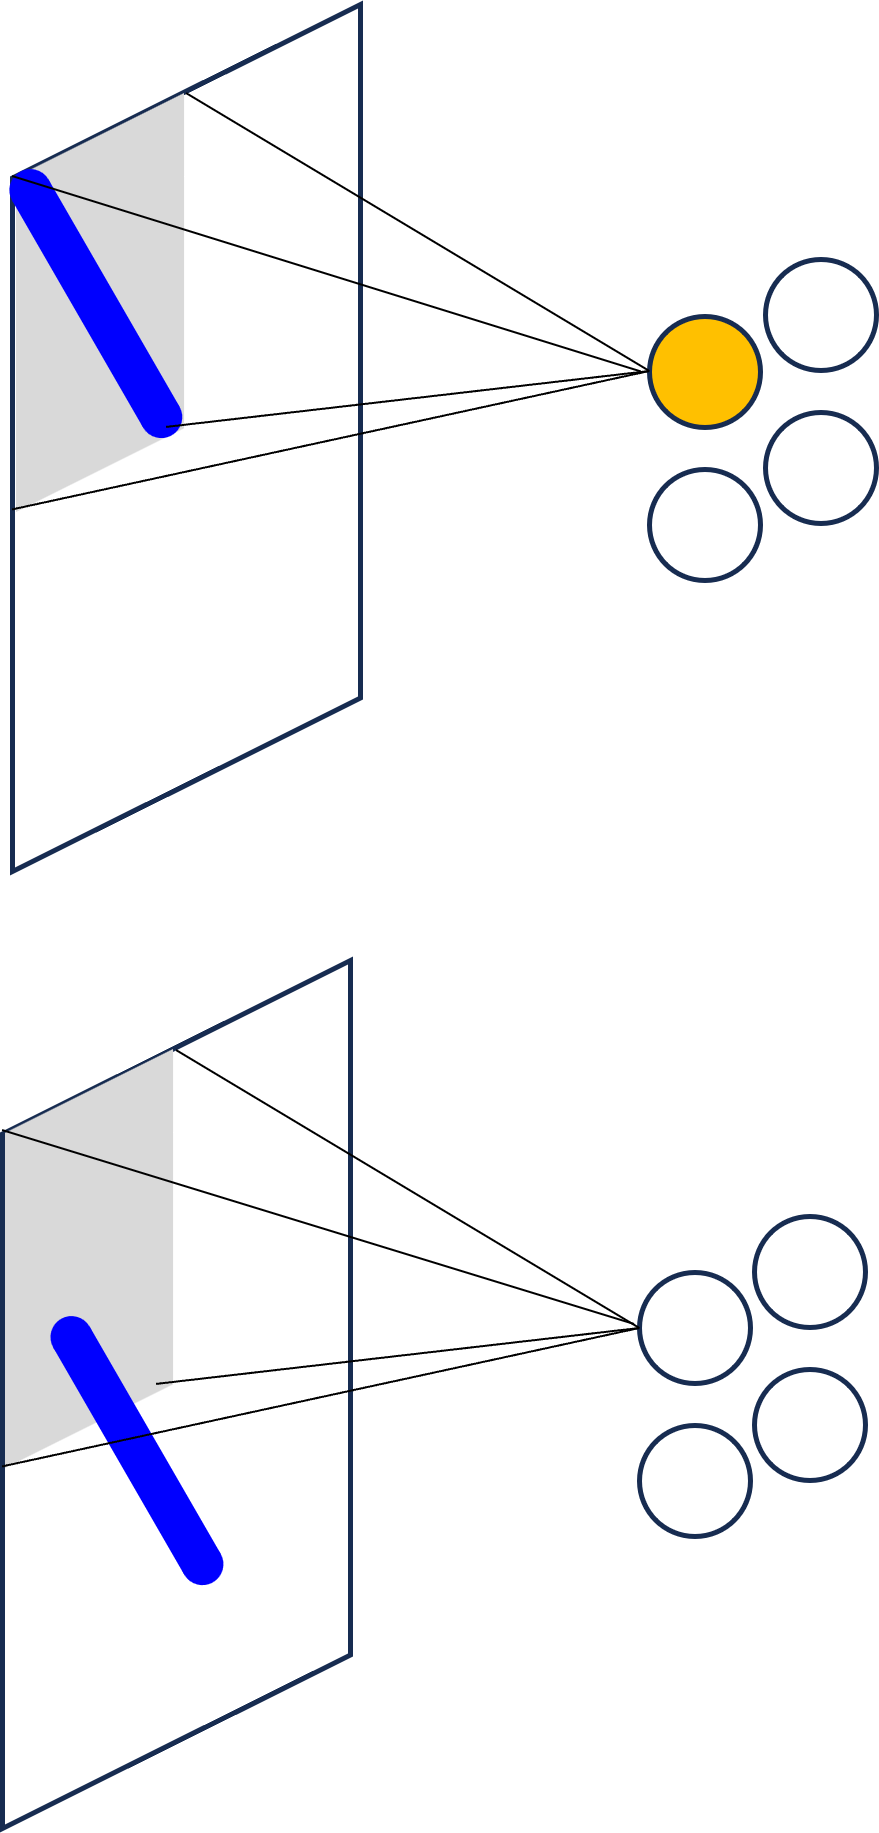
\includegraphics[height=8cm]{image/単純型細胞.png}
    \subcaption{単純型細胞}
    \label{単純型細胞}
  \end{minipage}
  \begin{minipage}[b]{0.5\linewidth}
    \centering
    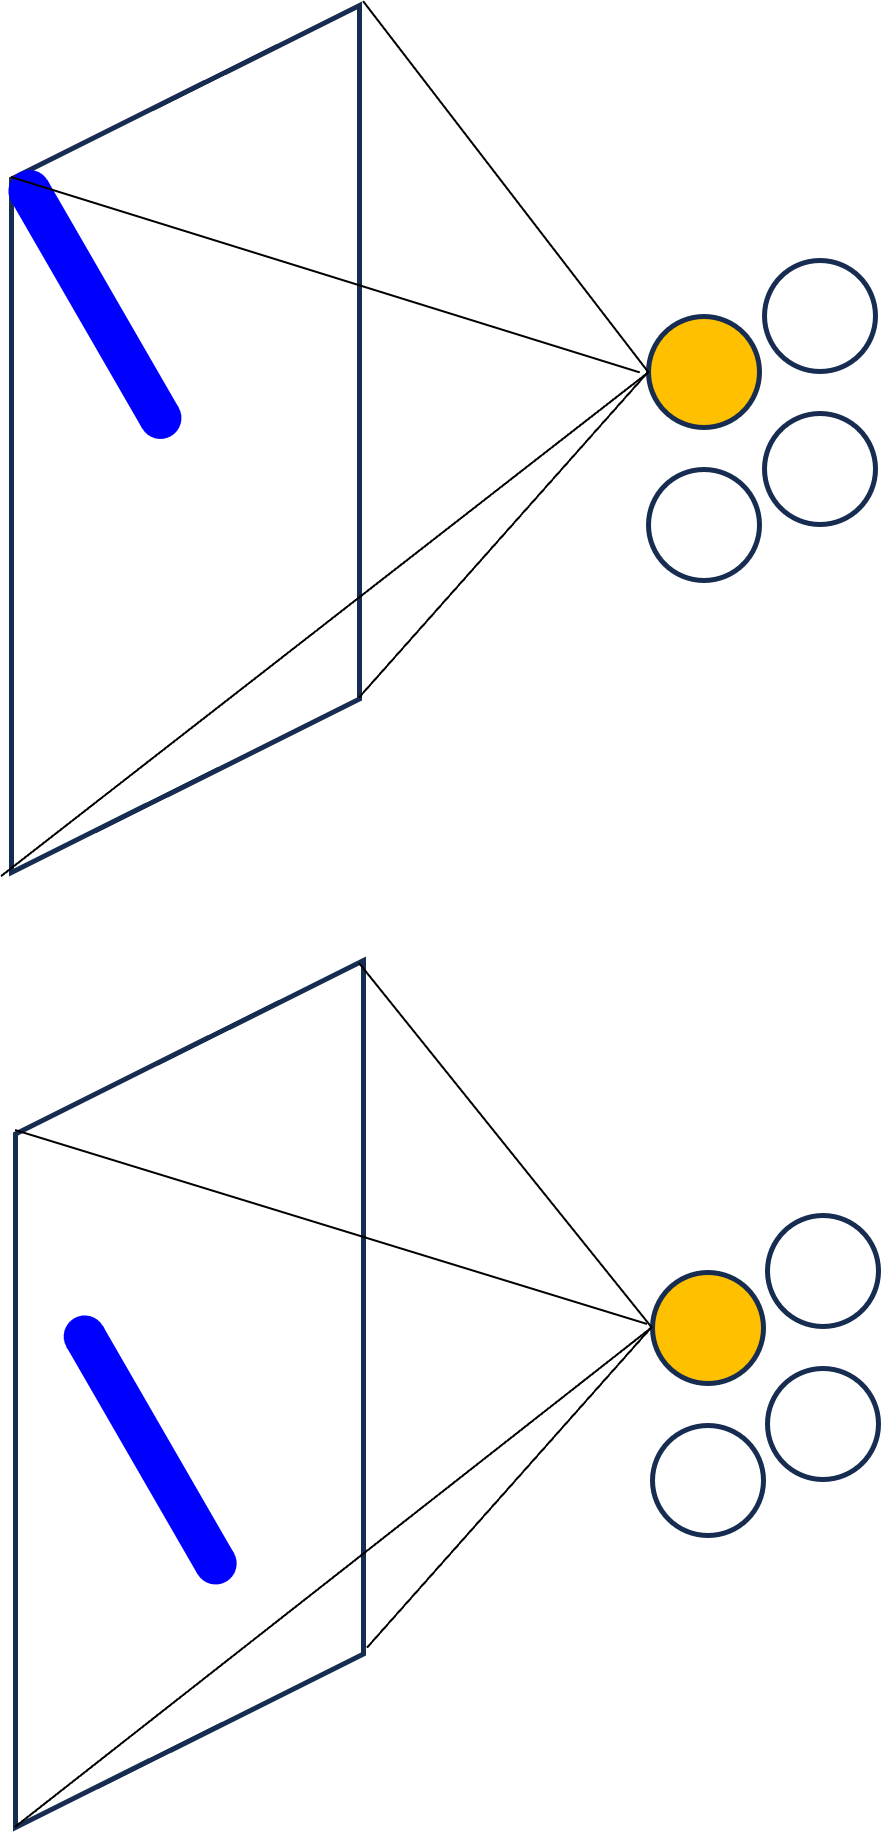
\includegraphics[height=8cm]{image/複雑型細胞.png}
    \subcaption{複雑型細胞}
    \label{複雑型細胞}
  \end{minipage}
  \caption{単純型細胞と複雑型細胞}
\end{figure}
多くの目をもつ生き物には視界に入っている物体を認識し,それが何であるかを判断することができる.なぜそのようなことができるのかというと,視覚情報からパターンを認識する高い能力が備わっているからである.どのようなメカニズムでパターンを認識しているか,その詳細はまだわかっていないが,ニューロンのネットワークがもつ構造に理由があると考えられている.\par
1958年にハーバード大学のヒューベルとウィーゼルは,猫の視覚野\footnote{視覚野とは,視覚情報の処理に関連する脳の部位である.大脳皮質の後頭葉という部分に位置する.}に特定の傾きをもつ線分を見せたときにだけ反応する細胞があることを発見した.さらにそのような細胞は2種類に大別できることを明らかにした.それらの細胞は単純型細胞と複雑型細胞とよばれ,受容野とよばれるニューロンを発火させるような入力を生じさせる領域の広さによって分別される.\par
図\ref{単純型細胞と複雑型細胞}は,網膜から視覚刺激を受け取ったときに,ニューロンがどう変化するかを示した概念図である.それぞれ左側ある四角が網膜の一部の領域に対応し,青で塗りつぶされた線分が視覚情報に対応する.そして,右側の4つの丸がニューロンであり,(a)は単純型細胞,(b)は複雑型細胞である.灰色で塗りつぶされた部分はそれぞれ左上のニューロンがもつ受容野で,見てわかるとおり単純型細胞における受容野は四角の一部の領域のみしか持たず,複雑型細胞は全領域を持っている.\par
単純型細胞(a)に注目しよう.左上の図では線分が受容野にすっぽりと収まっており,ニューロンが発火している.しかし左下の図のように,線分の位置がずれると,受容野に収まらなくなり発火しなくなってしまう.それに対して,複雑型細胞(b)は広い受容野をもつため,線分の位置がずれても発火し続けている.\par
2種類の細胞により,ある特定の位置にあるパターンと,ある領域内にあるパターンの2種類のパターンを検出することが可能になる.

\subsection{ニューラルネットワークと畳み込み}
畳み込みニューラルネットワークは,主に2種類に層からできている.1つ目は単純型細胞と類似のユニットからなる層で,局所的な受容野をもっている.パターン認識では,抽出すべきパターンが画像のどの位置に現れるかはあらかじめわからない.そこで図\ref{単純型細胞}のように,入力側の層を,局所的な受容野をもつ単純型細胞で覆う.これにより,どの局所受容野にパターンが現れても次層のユニットに活性が生じる.これまで考えてきた全結合型のニューラルネットワークと比べ,構造が疎になっていることに注目してほしい.このようにCNNでは重み行列がスパースになっている.\par
CNNがパターン抽出のためのモデルであるならば,パターンが現れる画像中の位置によってパターン認識能力が変化しては困る.それを防ぐには,どこの局所受容野と単純型細胞の結合も,すべて同じ重みを共有すればよい.つまり図\ref{単純型細胞}において同じ色の線で書かれた結合重みは,すべて同じパラメータを共有している.このようにすることで,学習中に訓練サンプルのある受容野に現れたパターンから学んだ結果を,ほかの位置に現れたパターンの抽出にも適用できるからである.したがって単純型細胞への入力はすべて同じ重み行列をもつため,結合の多さにもかかわらずパラメータの数は少数である.CNNにおいてこれを実現する層を畳み込み層と呼ぶ.\par
この一方,複雑型細胞は図\ref{複雑型細胞}のように,多数の単純型細胞の出力をとりまとめる役割を果たす.つまりパターン抽出には直接関与しない.そのためこの細胞へ入力する結合の重みは固定し,学習しないものとする.CNNにおいてこれを実現する層はプーリング層とよばれる.

\subsection{画像データの扱い}
\begin{figure}[H]
  \begin{center}
      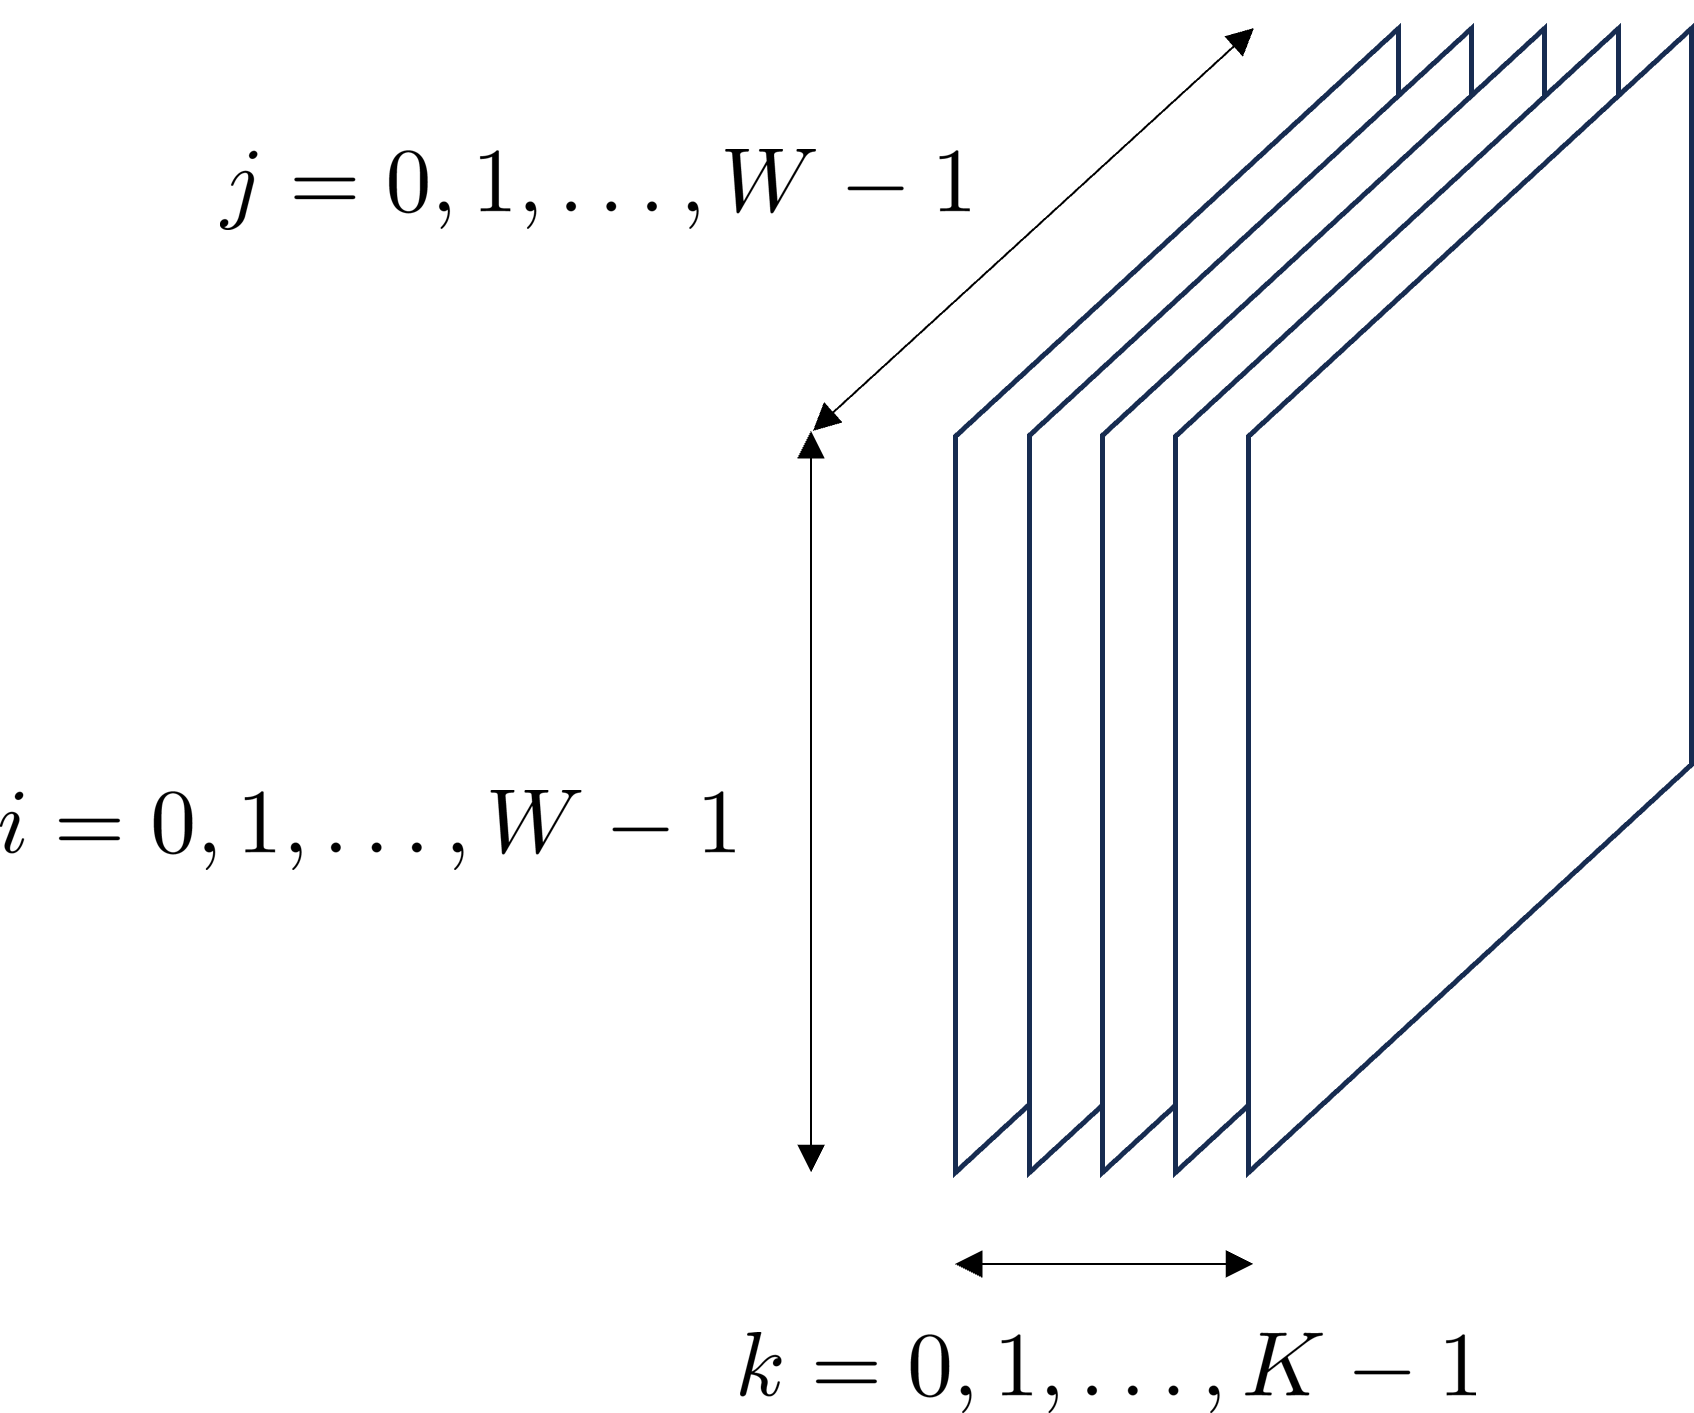
\includegraphics[height=6cm]{image/Kチャンネル画像.png}
      \caption{$K$チャンネルからなる$W \times W$画像}
      \label{Kチャンネル画像}
  \end{center}
\end{figure}
画像などの2次元データを用いて機械学習を行う場合,2次元のデータをわざわざ1次元のベクトルに変換してモデルに入力するよりも,2次元の構造を保ったままモデルに入力するほうが画像の2次元構造を最大限に活用できて便利である.ここでは,2次元画像データをどう扱うかについて説明する.\par
モノクロ画像の場合,画像データは実数画素値$x_{ij}$を持った2次元配列として表現することができる.添え字は画素の位置が$(i,j)$にあることを指定している.サイズが$W \times W$の画像の場合,
\begin{equation}
  i,j = 0,1,\dots,W-1
\end{equation}
の範囲で値をとる.0から数え始めているのは数式をシンプルにするためである.一般的な画像の場合,画像の位置$(i,j)$の自由度に加え,色成分などの自由度が付与される.このような自由度をチャンネルと呼ぶ.例としてRGBカラーを用いた画像では位置$(i,j)$に加え,赤,緑,青の3成分に対応した$k=0,1,2$の成分が加わり,画素値は$x_{ijk}$となる.一般化して$K$チャンネル$k=0,1,2,\dots,K$を考えると図\ref{Kチャンネル画像}のように,1枚の画像も,各チャンネルに応じた$K$枚の画像でできているとみなすことができる.

\subsection{畳み込み層}
まず1チャンネルの簡単な場合から考える.畳み込み層は行列入力$(z_{ij}^{(l-1)})$へフィルタを作用させる役割を果たす.そこでまずフィルタの役割を説明しよう.フィルタは入力よりも小さいサイズをもつ$H \times H$画像として定義する.その画素値を$h_{pq}$とする.画素の位置を表す添え字は
\begin{equation}
  p,q = 0,1,\dots,H-1
\end{equation}
の値をとる.$(z_{ij}^{(l-1)})$に対するフィルタ$(h_{pq})$の畳み込みを次の演算て定義する.
\begin{equation}
  u_{ij}^{(l)}
  = \sum_{p,q=0}^{H-1} z_{i+p,j+q}^{(l-1)} h_{pq} + b_{ij}
\end{equation}
ここで,$b_{ij}$はバイアスである.この畳み込み演算を$\ast$という記号で表すこともある.画像の画素$(i,j)$にフィルタの画素$(0,0)$が重なるようして両者を重ねる.そしてフィルタと重なった位置での両者の画素値の積$z_{i+p,j+q}^{(l-1)} h_{pq}$を計算する.この値を重なりの領域全体にわたって足し合わせたものを$u_{ij}^{(l)}$とする.これを畳み込み後の画像の$(i,j)$における画素値とする.この操作をフィルタが画像からはみ出ない範囲で行う.したがって畳み込める位置は$i,j=0,1,\dots,W-H$で与えられ,畳み込みの画像サイズは$(W-H+1)\times(W=H+1)$である.\par
\begin{figure}[H]
   \begin{center}
       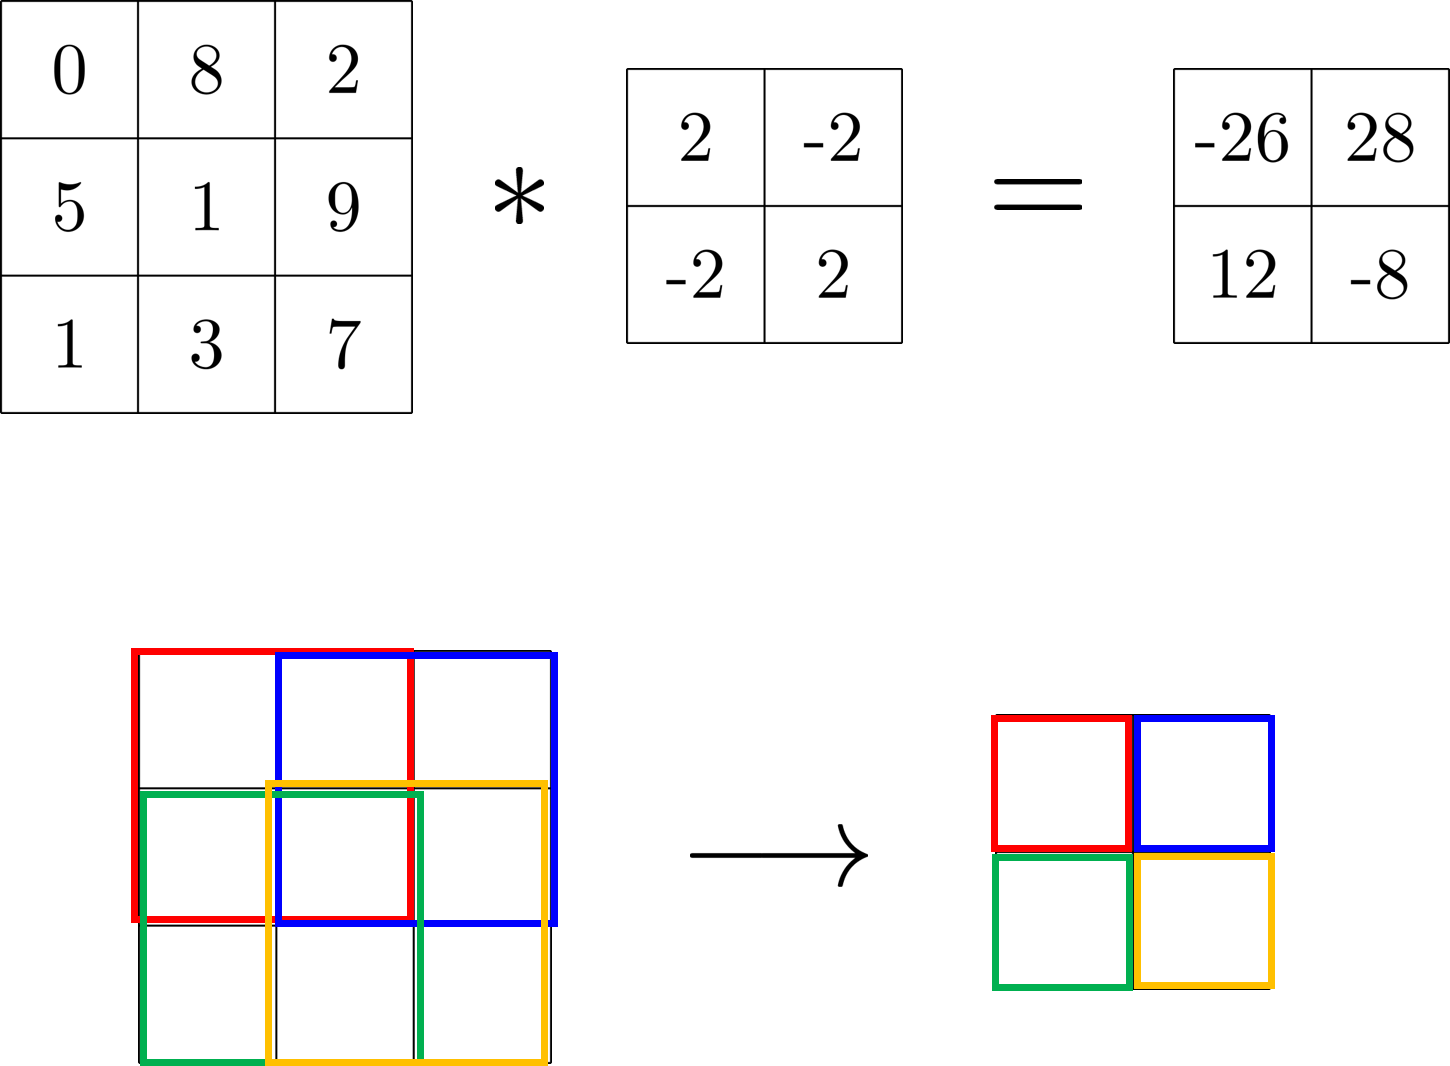
\includegraphics[height=5cm]{image/畳み込み演算の例.png}
       \caption{$3 \times 3$に対する$2 \times 2$フィルタの畳み込みの例.}
       \label{畳み込み演算の例}
   \end{center}
\end{figure}
フィルタは図\ref{畳み込み演算の例}のように作用し,画像からあるパターンを抽出する.このようにフィルタを畳み込むことで,画像から特定のパターンを抽出できる.CNNではパターンを抽出するのに適したフィルタは,我々が与えるのではなく訓練データから学習させる.つまり,CNNにおけるフィルタ$h_{pq}$が重みパラメータに他ならない.これらの重みは,かなり強く重み共有により正則化されている.というのもユニット$(a,b)$と次層のユニット$(i,j)$を結ぶ重みは,適当な整数$\Delta_{1,2}$で平行移動した場所のユニット$(a+\Delta_1,b+\Delta_2),(i+\Delta_1,j+\Delta_2)$間を結ぶ重みと全く同じだからである.つまり自由に動かせるパラメータは$H^2$しかない.\par
次に$K$チャンネル画像の対する畳み込みを考える.$K$チャンネル画像は$z_{ijk}^{(l-1)}$のように3つの添え字でラベルされているため,$W \times W \times K$画像とみなせる.このような画像を畳み込むには,同じチャンネル数を持つ$H \times H \times K$フィルタ$h_{pqk}$を用意する.そのうえで,各チャンネルごとに先ほどの畳み込みを行い,その後同じ位置の画素は全チャンネルにわたって足し上げてしまう.その結果得られる次の$(W-K+1)\times(W-K+1)$画像が畳み込みの結果となる.
\begin{equation}
  u_{ij}^{(l)}
  = \sum_{k=0}^{K-1}\sum_{p,q=0}^{H-1} z_{i+p,j+q,k}^{(l-1)} h_{pqk} + b_{ij}
\end{equation} \par
多チャンネルのフィルタが1種類しかない場合,このように畳み込み後の画像は1種類しかない.畳み込み後も多チャンネル画像が欲しいならば,ほしいチャンネル数$M$に応じて$K$チャンネルのフィルタを$M$種類用意する.つまり
\begin{equation}
  u_{ijk}^{(l)}
  = \sum_{k=0}^{K-1}\sum_{p,q=0}^{H-1} z_{i+p,j+q,k}^{(l-1)} h_{pqkm} + b_{ijm}
  \label{畳み込み計算式}
\end{equation}
のように畳み込めばよい.\par
畳み込み層の最終的な出力は,この画像に活性化関数$f$を作用させたものになる.
\begin{equation}
  z_{ijm}^{(l)}
  = f(u_{ijm}^{(l)})
  \label{畳み込み計算式2}
\end{equation}
畳み込み層からの出力のことを特徴量マップともいう.活性化関数としては,最近はよくReLU関数が用いられる.\par
このように$W \times W \times K$画像$(Z_{ijk}^{(l-1)})$から$(W-H+1) \times (W-H+1) \times M$の画像$(Z_{ijm}^{(l)})$を出力するのが畳み込み層である.とはいえ,式(\ref{畳み込み計算式}),式(\ref{畳み込み計算式2})からわかるように,この層は$w \times W \times K$個のユニットからなる$l-1$層と$(W-H+1) \times (W-H+1) \times M$個のユニットの$l$層を,共有させた重み${h_{pqkm}}$で結合させた普通の順伝播層ともみなせる.したがって通常の誤差逆伝播法を用いることで,重みであるフィルタを学習することができる.
\subsubsection{ストライド}
これまでフィルタは1目盛りずつ動かして,パターン抽出を行っていた.しかしもう少し大雑把に画像の特徴を捉えたい場合には,必ずしも1画素ずつ動かして一のパターンをこまめに調べる必要はない.そこでCNNではストライドという方法がとられる.ストライド$S$とは,画素を$S-1$個余分に飛ばしてフィルタを動かしていくことを意味する.フィルタが$S$画素動くごとに1回畳み込みを行うストライド$S$では,畳み込みの式は次のようになる.
\begin{equation}
  u_{ijk}^{(l)}
  = \sum_{k=0}^{K-1}\sum_{p,q=0}^{H-1} z_{Si+p,Sj+q,k}^{(l-1)} h_{pqkm} + b_{ijm}
\end{equation}
このようなストライドを用いた場合の畳み込み後の画像のサイズは
\begin{equation}
  \left(\left\lfloor \frac{W-H}{S} \right\rfloor + 1\right) \times \left(\left\lfloor \frac{W-H}{S} \right\rfloor + 1\right)
\end{equation}
となる.ここで床記号$\lfloor x \rfloor$は$x$を超えない最大の整数を意味する.このようにストライドを用いることで畳み込み後の画像サイズを小さくすることができる.しかしあまり大きなストライドを用いるとこまめな構造を捉えられず,捉えるべきパターンをストライドのせいでスキップしてしまう可能性もある.したがって考えるデータの性質に応じて,ストライドの設定には注意を払う必要がある.

\subsubsection{パディング}
畳み込みをすると必ず画像サイズが小さくなってしまう.特にフィルタサイズやストライドが大きいときはその縮小が顕著である.これはフィルタを重ね合わせる際に,元の画像からはみ出せないという制約に起因している.しかし,画像処理では,画像サイズが小さくなると技術的に都合がよくない状況も存在する.\par
そのような状況の場合,パディングという手法を用いることで,畳み込み後の画像サイズをある程度大きくすることができる.パディング$P$とは,元の画像の周りに厚さ$P$のふちを加える操作である.したがってストライド$S$,パディング$P$の畳み込みをした後の画像サイズは
\begin{equation}
  \left(\left\lfloor \frac{W-H+2P}{S} \right\rfloor + 1\right) \times \left(\left\lfloor \frac{W-H+2P}{S} \right\rfloor + 1\right)
\end{equation}
となる.パディングには加えた画素にどのような値を入れるかによって複数種類が存在する.よく使われるのがゼロパディングで,増やした画素すべてに画素値0を代入する.\par
ゼロパディングはとても簡単な手法であるが,0を用いるためどうしても畳み込み後の画像は周辺部の画素値が小さくなり,暗くなってしまう.そこで,ゼロパディング以外にも,元の画像の画素値を用いてパディングする方法がある.名前だけ紹介すると周期パディングや反射パディングである.

\subsection{プーリング層}
次に複雑型細胞に対するプーリング層について説明する.この層の役割は,畳み込み層で捉えた局所的なパターンを,その位置がある程度移動しても捉えられるようにすることであった.入力位置の平行移動に対してロバストにするためには,各位置で局所的パターンを抽出して単純型細胞からの出力を合算すればよかった.\par
プーリングではまず,$W \times W \times K$入力画像$z_{ijk}^{(l-1)}$の各チャンネルに対し,各画素位置$(i,j)$を中心とした$H \times H$の大きさの領域$\mathcal{P}_{ij}$を考える.ただし画像はパディングしておき,どの点に対しても$\mathcal{P}_{ij}$の領域を考えられるようにしておく.そして$\mathcal{P}_{ij}$中の画素値から,その領域での代表的な画素$u_{ij}^{(l)}$を決定する.代表値を決める方法は複数あるが最大プーリングでは,領域内の最も大きな画素値を代表値として取り出す.
\begin{equation}
  u_{ijk}^{(l)}
  = \underset{(p,q) \in \mathcal{P}_{ij}} {\operatorname{max}} z_{pqk}^{(l-1)} 
\end{equation}
また,最大値の代わりに,領域内の平均を用いる平均プーリングという方法もよく使われる.
\begin{equation}
  u_{ijk}^{(l)}
  = \frac{1}{H^2} \sum_{(p,q) \in \mathcal{P}_{ij}} z_{pqk}^{(l-1)} 
\end{equation}\par
なおプーリング層の役割は畳み込み層の出力を束ねるだけであるため,重みの学習は行わない.したがって学習中もプーリングの式は一切変更されない.



\section{勾配降下法}
ニューラルネットワークの学習は損失関数の最小化によって行われる.つまり,ネットワークパラメータの空間上でスカラー関数$L(\bm{\theta})$の最小値を探すという最適化問題を解くことになる.
\begin{equation}
  \bm{\theta}^* = \underset{\bm{\theta}} {\operatorname{argmin}} \ L(\bm{\theta})
\end{equation}
損失関数は基本的に多くのパラメータを含む複雑な関数であるため,このような最適化問題を厳密に解くことはできない.そのため,計算機によって数値的に近似解を求めることになる.\par

\subsection{勾配降下法}
誤差関数$E(\bm{\theta})$の最小点を見つける手法のうち,最も直観的で単純なアイデアは図\ref{勾配降下法イメージ図}のように,誤差関数のグラフの形状をした凹みにおいて.上のほうからボールを転がり落してボールの一番低いところにたどり着くまで待つ方法である.これがまさに勾配降下法の考え方である.\par

\begin{figure}
  \begin{center}
    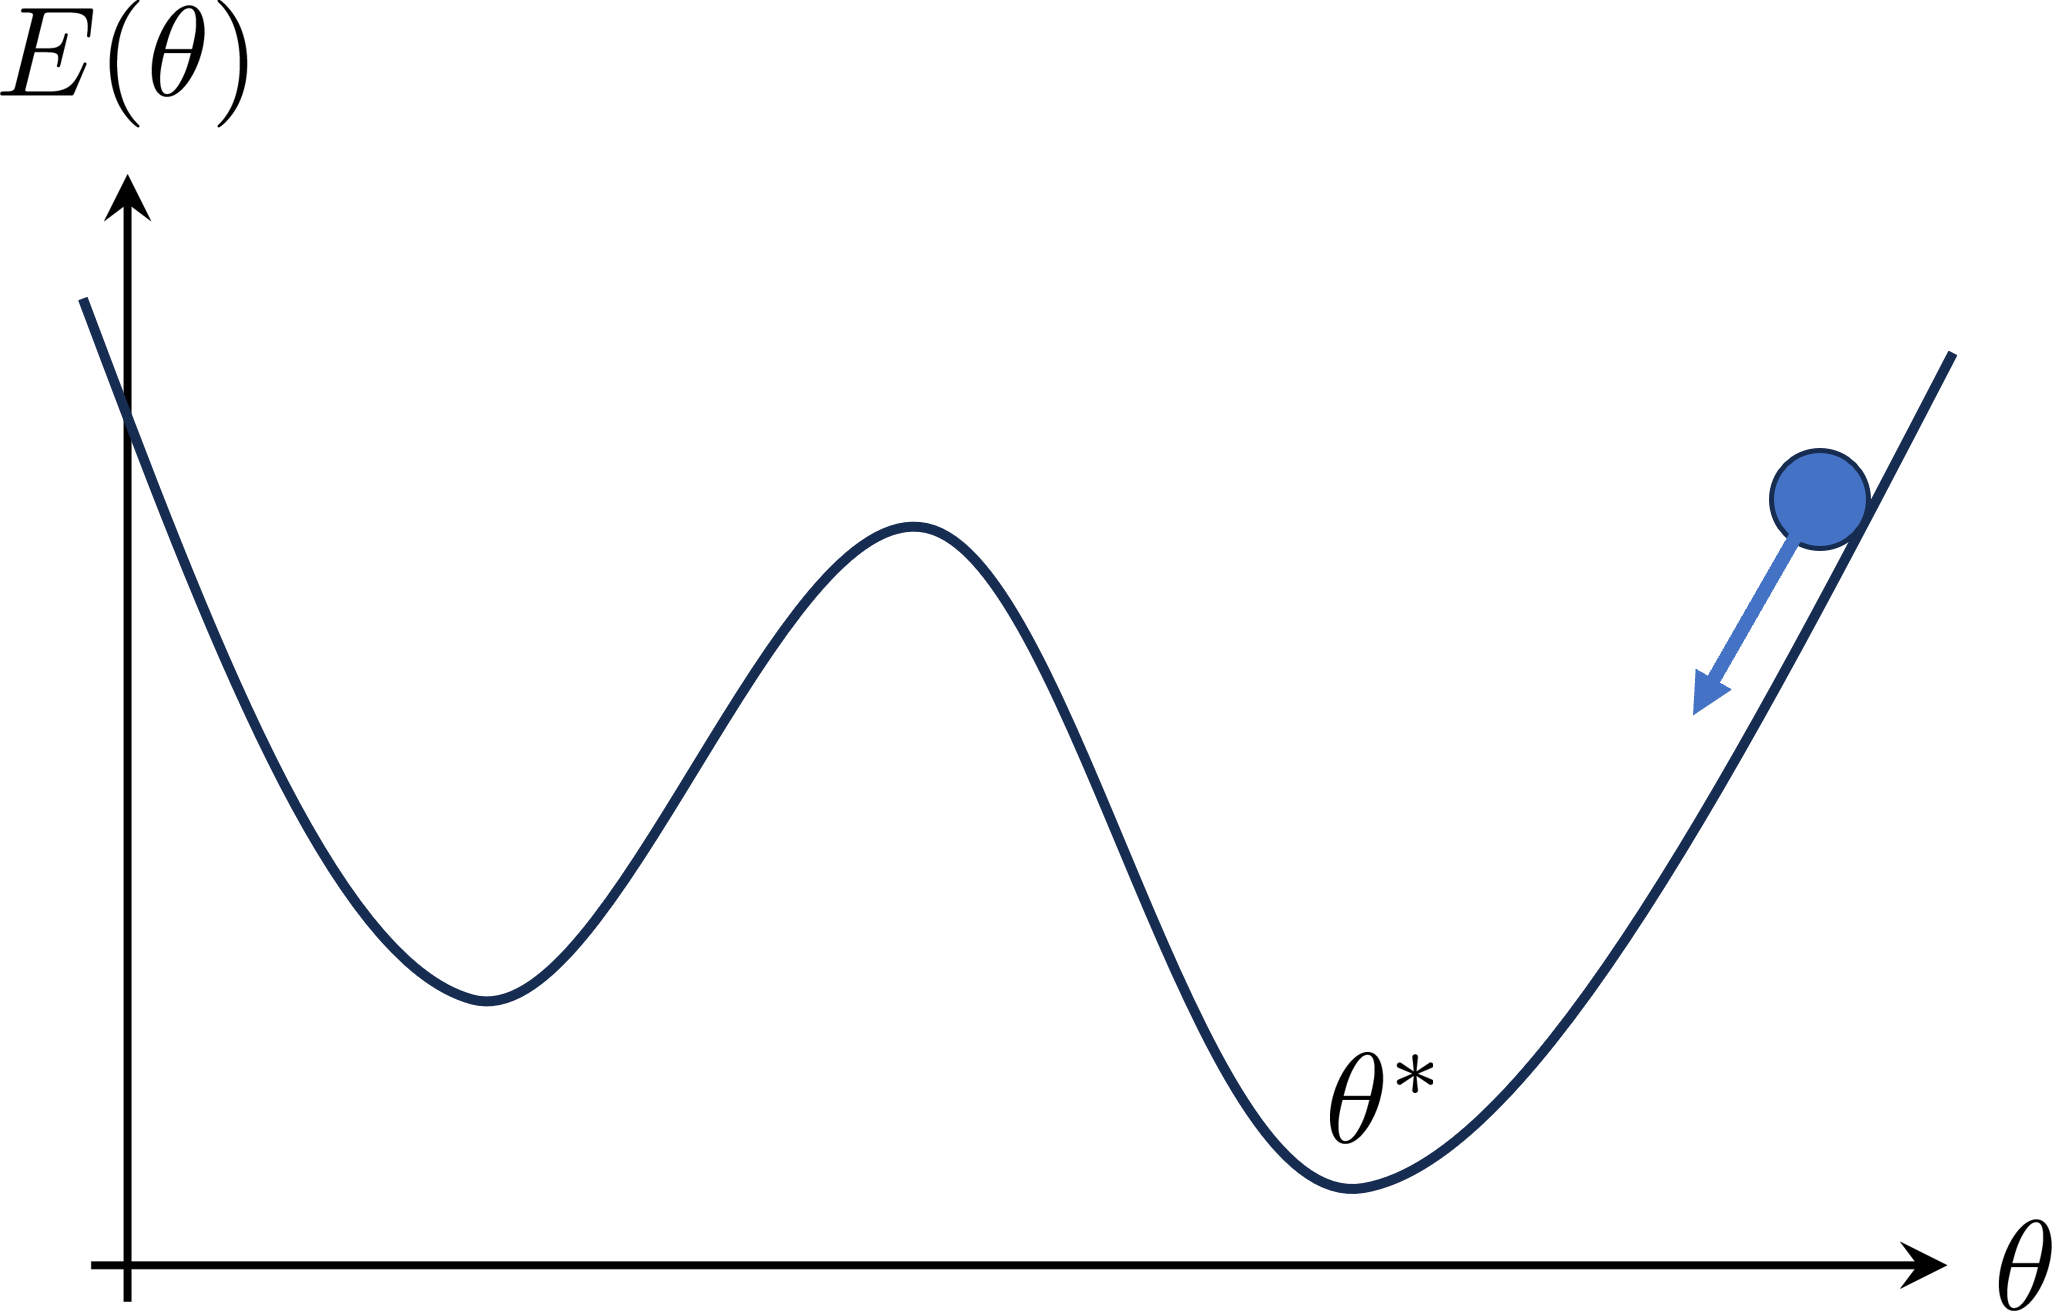
\includegraphics[height=5cm]{image/gradient_decent.png}
    \caption{勾配降下法による極小値の見つけ方}
    \label{勾配降下法イメージ図}
  \end{center}
\end{figure}

ボールを転がり始めさせる位置に対応して,勾配降下法ではパラメータの初期値$\theta^{(0)}$を用意する.この初期値から始めて,坂道でボールを転がすような操作を,離散的な時間$t=0,1,2,\dots$を用いて定式化しよう.坂を転がすというのは,現在位置におけるグラフの勾配
\begin{equation}
  \nabla E(\bm{\theta})
  = \frac{\partial E(\bm{\theta})}{\partial \bm{\theta}}
  \equiv \left(  \frac{\partial E(\bm{\theta})}{\partial \theta_1}, \cdots,  \frac{\partial E(\bm{\theta})}{\partial \theta_D} \right)
\end{equation}
の逆方向に動かすことを意味する.ここで表記を簡単にするため,ニューラルネットワークの重みパラメータを下付き添え字$\theta_1,\theta_2,\dots,\theta_D$でラベル付けした.$D$はニューラルネットワークの全パラメータ数である.すると時刻$t$で位置$\bm{\theta^{(t)}}$にあったボールを勾配の逆方向に動かす際のルールは次のようになる.
\begin{equation}
  \bm{\theta^{(t+1)}} = \bm{\theta^{(t)}} + \Delta \bm{\theta^{(t)}} , \ \  \Delta \bm{\theta^{(t)}} = - \eta \nabla E\left( \bm{\theta}^{(t)} \right)
\end{equation}
右辺で次時刻の$\theta^{(t+1)}$を定義する操作を$t=0,1,2,\dots$と順次繰り返していくことで,どんどんと誤差関数のグラフの底のほうに降りていくことができる.$1$ステップでの移動距離$\Delta \bm{\theta^{(t)}}$の大きさを決めるハイパーパラメータ$\eta$は学習率(learning late)と呼ばれる.この操作が収束し,もはや動けなくなった点が勾配が消える極小値である.ここでいう収束とは,計算機の数値制度の範囲内でもはや$\theta^{(t)}$の変化が見られなくなる状況のことである.\par
学習率の取り方には一般論は存在せず,現状ではトライアルアンドエラーに基づかざるを得ない.しかし学習率をあまり大きくすると,$1$ステップの刻みが荒らすぎて誤差関数の形状をうまく捉えられずに,収束に問題を起こす.その一方であまり小さくしすぎると学習が一向に進まなくなる.したがって,程よい大きさの学習率を見つけることが,学習をうまく進めるために重要となる.\par

\subsection{局所的最小値の問題}
いままでは最小値と極小値の区別に注意を払わなかった.誤差関数が下に凸な関数である簡単な状況では任意の極小値は必ず最小値に一致するので区別する必要がない.しかしながらディープラーニングにおける誤差関数は一般的にとても複雑な非凸関数なので,本当の極小値である大域的極小値以外にも,膨大な数の局所的極小値をもつ.\par
さらにニューラルネットワークには高い対称性と極小値の重複がある.例えば,第$l$層の2つのユニット$j=1,2$に注目すると,この2つのユニットを入れ替えても最終層の出力は変わらない.なぜなら,$\theta_{1i}^{(l)},\theta_{k1}^{(l+1)}$と$\theta_{2i}^{(l)},\theta_{k2}^{(l+1)}$をすべて同時に入れ替えれば何もしていないことと同じになるからである.各層でこのような入れ替えは${}_{d_l} C_2$通りだけある.したがってニューラルネットワーク全体では$\prod_l {}_{d_l} C_2$通りだけの入れ替え対称性があることがわかる.つまり,局所的極小値が1つでも見つかれば,自動的に$\prod_l {}_{d_l} C_2$個の極小値が重複して存在することになる.このように,深層モデルでは極小値の数は膨大になる.\par
このような場合,勾配降下法で大域的極小値を探すのは,干草の中から針を探すようなものである.したがってディープラーニングでは極小値にはたどり着けても,真の極小値にはまずたどり着けない.通常の機械学習の文脈ではこれは深刻な問題であり,局所的最小値の問題や局所的最適解の問題と呼ばれる.\par
ところが不思議なことに,ディープラーニングでは真の最小値を見つけずとも,誤差関数のよい極小値さえ見つけられれば十分であると予想されている.これはディープラーニングを他の機械学習とは一線を画す画期的な手法にしていると同時に,ディープラーニングにおける大きな謎の1つである.この点に関しては現在でもさまざまな研究がなされている.\par

\subsection{確率的勾配降下法}
ディープラーニングが真の最小値を必要としないとはいっても,誤差関数の値があまりに大きい臨界点にはまり込んでしまっては全く使い物にならない.そこで臨界点にトラップされることをできるだけ回避するためにランダムな要素を取り入れて,はまり込んだ場所から弾き出す効果を生み出すことで勾配降下法を改良していく.\par
ランダムな要素を入れるためには,学習の仕組みを復習する必要がある.学習データ$\mathcal{D}=\{(\bm{x}_n,\bm{y}_n)\}_{n=1,2,\dots,N}$が与えられたとき,誤差関数は各学習サンプル要素$(\bm{x}_n,\bm{y}_n)$で計算した誤差の和として表現できた.
\begin{equation}
  E(\bm{\theta}) = \frac{1}{N}\sum_{n=1}^{N}E_n(\bm{\bm{\theta}}) \label{勾配降下法}
\end{equation}
例えば平均二乗誤差を用いるならば
\begin{equation}
  E_n(\bm{\bm{\theta}}) = \frac{1}{2}\left( \bm{y}(\bm{x}_n ; \bm{\theta}) - \bm{y}_n \right)^2
\end{equation}
であり,$K$クラス分類ならば交差エントロピー
\begin{equation}
  E_n(\bm{\bm{\theta}}) = - \sum_{k=1}^{K} t_{nk}\log{y_k(\bm{x}_n ; \bm{\theta})}
\end{equation}
を用いた.先ほどの勾配降下法では式(\ref{勾配降下法})のように毎回の更新ですべての訓練サンプルを用いていた.このような方法はバッチ学習と呼ばれる.\par
しかし勾配によるパラメータ更新は何回も繰り返すことになるので,1回の更新で毎回すべてのサンプルを用いる必要がない.各時間ステップで,一部の訓練サンプルだけを用いる方法をミニバッチ学習という.ミニバッチ学習ではまず,各時間$t$で用いる訓練サンプルの部分集合$\mathcal{B}^{(t)}$を用意する.この$\mathcal{B}^{(t)}$のことをミニバッチと呼び,通常は学習前にランダムに作成しておく,そして時刻$t$における更新ではミニバッチ上で平均した誤差関数
\begin{equation}
  E^{(t)}(\bm{\theta}) = \frac{1}{\mathcal{B}^{(t)}} \sum_{n\in \mathcal{B}^{(t)}} E_n(\bm{\theta})
\end{equation}
を用いる.ここで$n\in \mathcal{B}^{(t)}$はミニバッチに含まれる訓練サンプルのラベルを表し,$|\mathcal{B}^{(t)}|$はミニバッチの中のサンプル要素の総数である.これを用いてバッチ学習同様,パラメータを更新する.
\begin{equation}
  \bm{\theta^{(t+1)}} = \bm{\theta^{(t)}} + \Delta \bm{\theta^{(t)}} , \ \  \Delta \bm{\theta^{(t)}} = - \varepsilon \nabla E^{(t)}\left( \bm{\theta}^{(t)} \right)
\end{equation}
特に各時刻のミニバッチに1つの訓練サンプルしか含まない$|\mathcal{B}^{(t)}|=1$という場合をオンライン学習や確率的勾配降下法と呼ぶ.\par
ミニバッチ学習ではランダムにミニバッチを選んだことにより,時刻ごとに誤差関数$E^{(t)}(\bm{\theta})$の形もランダムに変化する.したがって,ずっと同じ関数$E(\bm{\theta})$を使い続けるバッチ学習とは違い,望ましくない臨界点にはまり込む可能性がかなり小さくなる.これがミニバッチ学習が重宝される大きな理由である.\par
さらにサンプルを効率的に使う観点からもミニバッチは好まれる.訓練データのサイズが大きくなると,似たようなサンプルが含まれる可能性が高くなる.そこで訓練データ集合全体ではなく,ミニバッチを使用することで,1回の更新ステップにおいて似たデータを重複して使用する無駄が省けるようになる.\par
またミニバッチでの勾配降下法では,各勾配$\nabla E_n(\bm{\theta})$の計算が独立で容易に並列化できる.したがって,コアのたくさんあるGPGPUなどの並列計算環境がある場合には,ある程度のサイズのミニバッチを利用するほうが理にかなっている.

\subsection{ミニバッチの作り方}
(ミニ)バッチ学習では,学習時間をエポック(epoch)という単位ごとに分けて考える.1エポックという単位は,訓練データ全体を1周すべて使い切る時間単位を意味する.\par
まずはじめのエポックでは,データを適当なサイズのミニバッチにランダムに分割する.そして,これらのミニバッチを用いて勾配を更新していく.すべてのミニバッチを使い切ったら,このエポックは終了になる.しかし通常は,1エポックでは不十分で,次のエポックに進み,改めてランダムにミニバッチを作り,同じプロセスを繰り返していく,そして,誤差関数が十分小さくなるまでエポックを繰り返したら,学習終了になる.\par
また,バッチ学習では毎回データを使い切るため,エポックと更新時間は一致する.

\section{改良された勾配降下法}
\subsection{勾配降下法の課題}
前節で勾配法には,局所最適解の問題があることをみたが,それ以外にも多くの課題がある.\par
図\ref{勾配法の課題}(a)のように誤差関数が深い谷を作っている状況を考える.このような谷に対して勾配降下法で勾配の方向にパラメータを更新するだけでは谷に沿って激しく振動するばかりで,いつまでたってもパラメータが収束しない.\par
一方,図\ref{勾配法の課題}(b)のように,平らな領域があった場合を考える.このような場所はプラトーと呼ばれる.一度プラトーに入り込んでしまうと勾配が消えるため,パラメータの更新も止まってしまう.ミニバッチアドでランダムな要素を入れたとしても,深層学習の誤差関数に現れるプラトーは学習の進みを遅くする原因になってしまう.\par
さらに,図\ref{勾配法の課題}(c)のような急に切り立った絶壁の存在も危険である.それまで緩やかな坂を下ってきたとしても,絶壁に当たった瞬間に極めて大きな勾配によって吹き飛ばされてしまう.
\begin{figure}[htbp]
  \begin{minipage}[b]{0.3\linewidth}
    \centering
    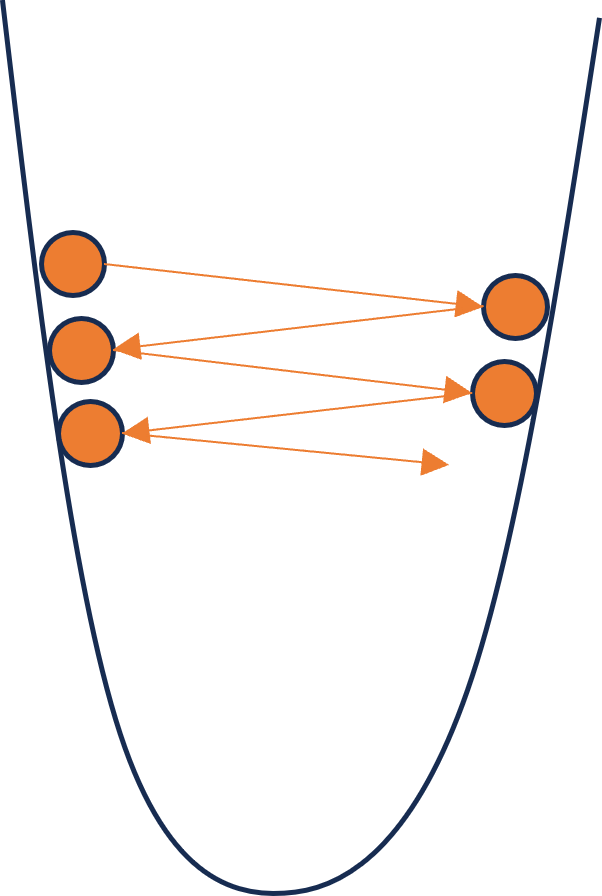
\includegraphics[keepaspectratio, scale=0.5]{image/勾配法課題(a)}
    \subcaption{}
  \end{minipage}
  \begin{minipage}[b]{0.3\linewidth}
    \centering
    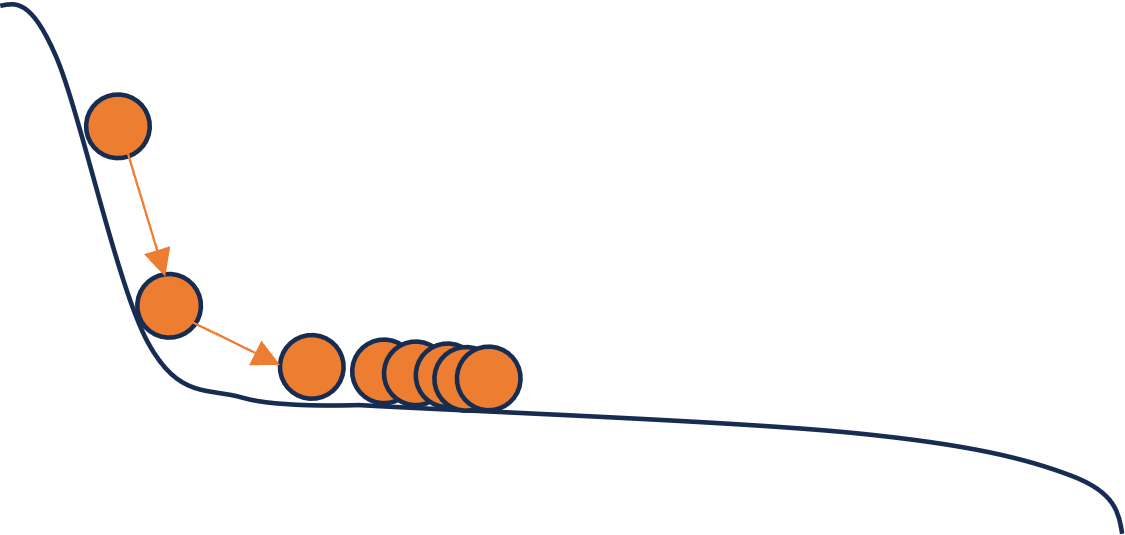
\includegraphics[keepaspectratio, scale=0.5]{image/勾配法課題(b)}
    \subcaption{}
  \end{minipage}
  \begin{minipage}[b]{0.3\linewidth}
    \centering
    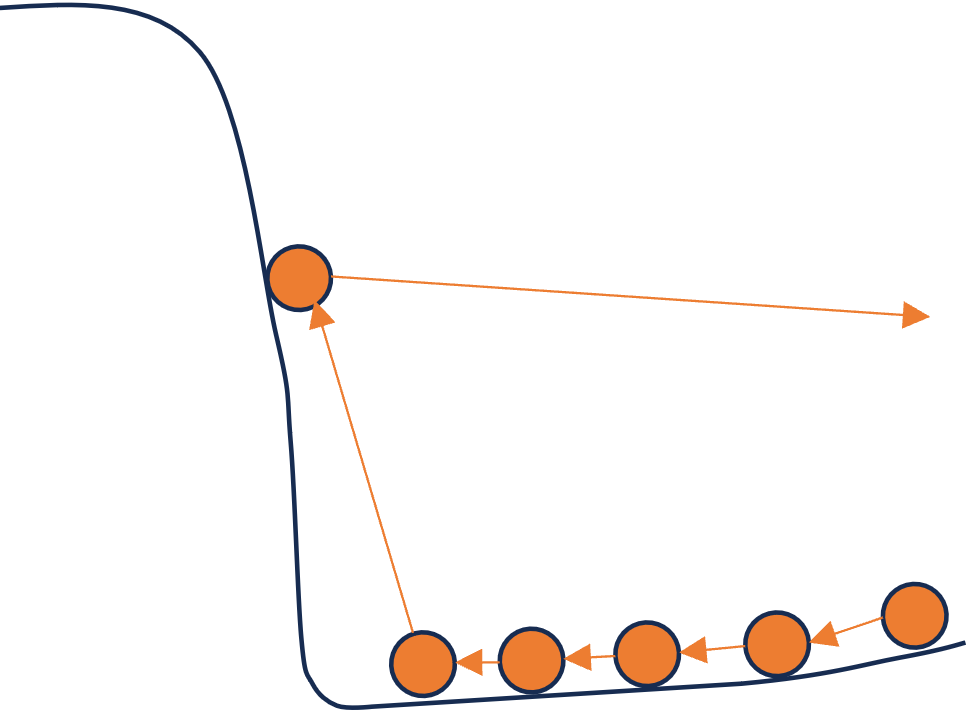
\includegraphics[keepaspectratio, scale=0.5]{image/勾配法課題(c)}
    \subcaption{}
  \end{minipage}
  \caption{(a)谷で振動.(b)プラトーで停止.(c)絶壁で反射}
  \label{勾配法の課題}
\end{figure}


\subsection{モーメンタム法}
振動による問題を改善する手法としてモーメンタム(momentum)というものがある.モーメンタムは「慣性」とも訳され.前時刻での勾配の影響を引きずらせることで振動を防ぐことができる.\par
振動の原因は,深い谷の底周りで急激な勾配が正負交互に発生するためであった.そこで,1個前のステップでの勾配の影響を,現在の勾配に加えることを考える.前回のパラメータ更新量$\Delta \bm{\theta}^{(t-1)}$が負の値で,現在の勾配$\nabla E(\bm{\theta}^{(t)})$が正の大きな値であるとする.すると前回の更新量を現在の勾配に少し加えることで,図\ref{モーメンタム法による勾配抑制図}のように今回の更新量$\Delta \bm{\theta}^{(t)}$を比較的小さな値に抑えることができる.つまり,手法で勾配が大きく正負に振れること防ぐことができる.
\begin{align}
  \bm{\theta}^{(t+1)}
   & = \bm{\theta}^{(t)} + \Delta \bm{\theta}^{(t)}                              \\
  \Delta \bm{\theta}^{(t)}
   & = \mu \Delta \bm{\theta}^{(t-1)} - (1-\mu) \eta \nabla E(\bm{\theta}^{(t)}) \label{モーメンタム法}
\end{align}
\begin{figure}
  \begin{center}
    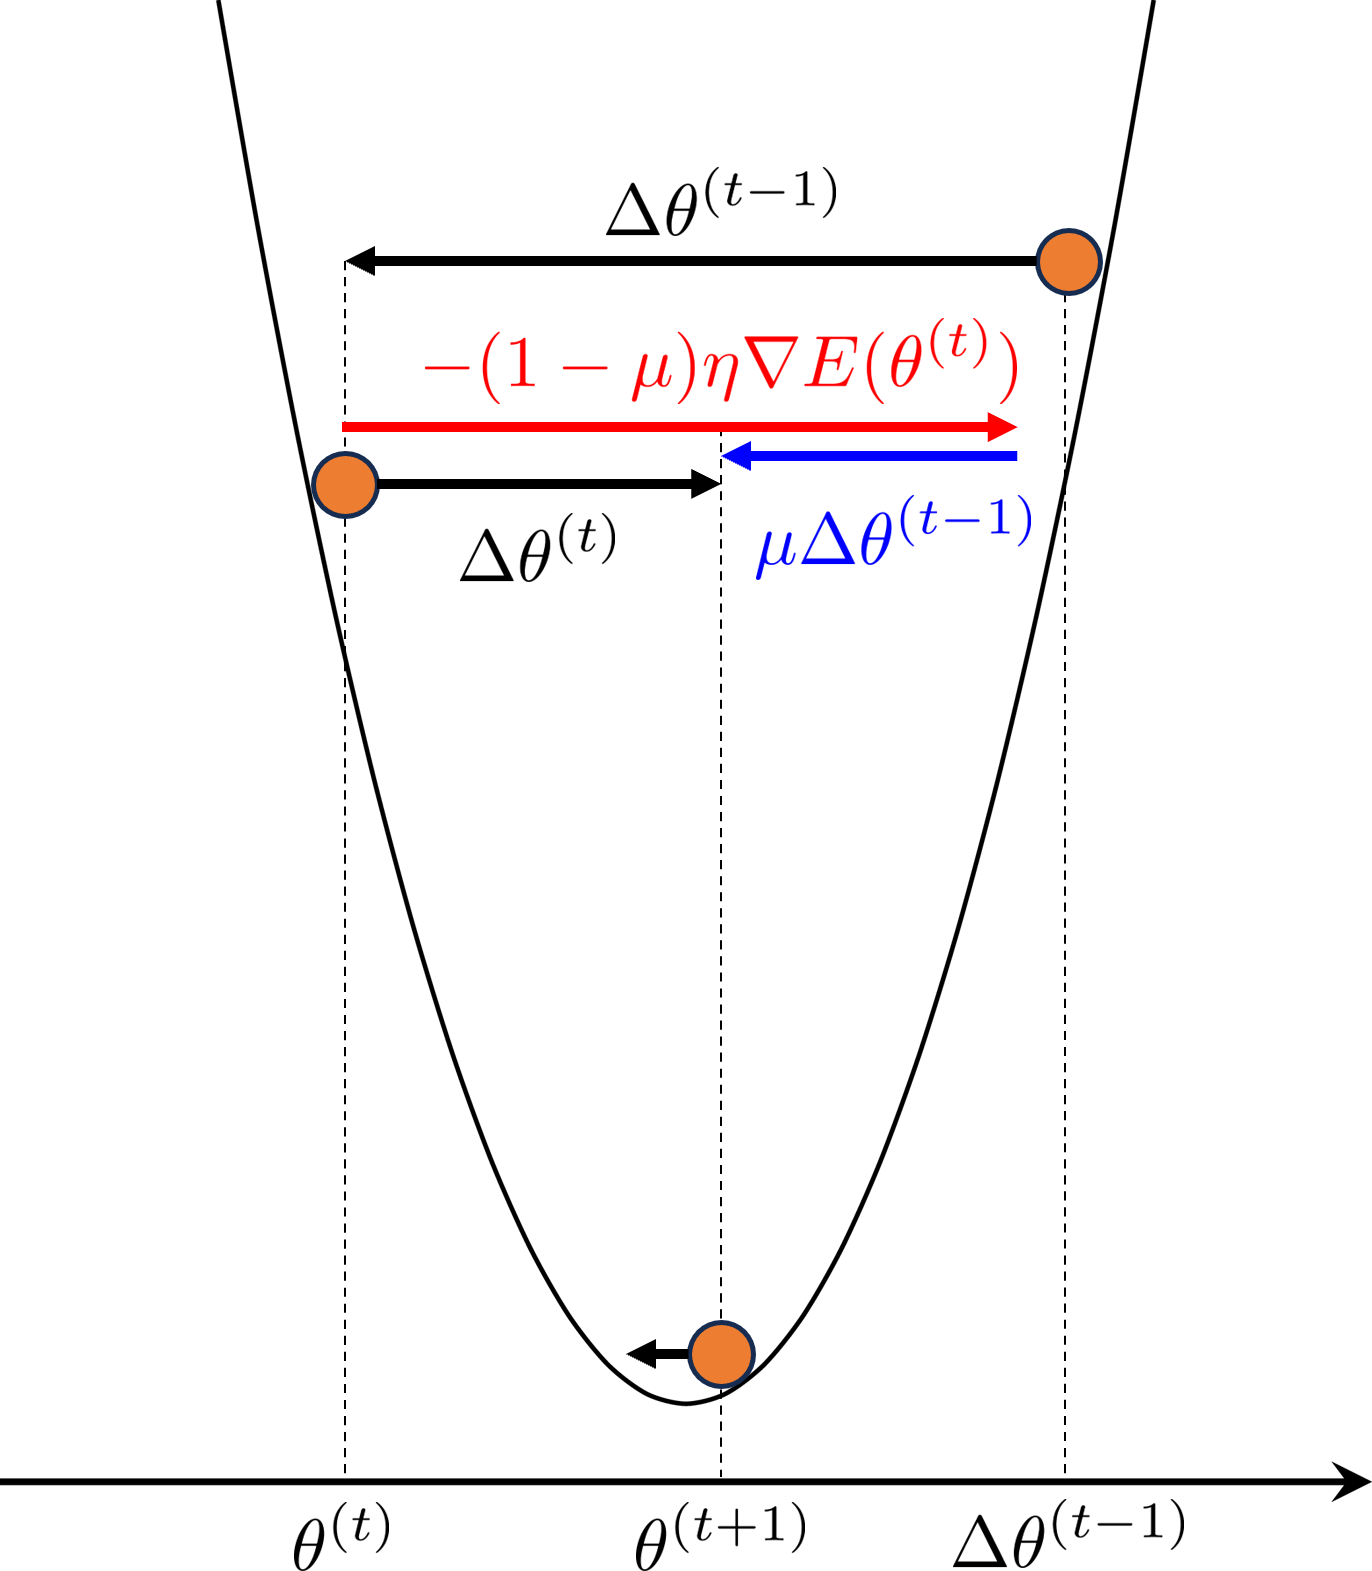
\includegraphics[height=8cm]{image/モーメンタム法.png}
    \caption{モーメンタム法による谷での振動の抑制}
    \label{モーメンタム法による勾配抑制図}
  \end{center}
\end{figure}
初期値は$\Delta \bm{\theta}^{(0)} = 0$にとる.また,$\mu$は比較的$1$に近い$0.5 \sim 0.99$程度の値をとる.\par
モーメンタム法は振動を防ぐ効果だけではなく,普通の斜面において勾配法でのパラメータ更新の加速も可能にする.これを見るために誤差関数の傾き$\nabla E(\bm{\theta}^{(t)})$が一定の領域を考える.この場合,式(\ref{モーメンタム法})の終端速度は$\Delta \bm{\theta}^{(t)} = \Delta \bm{\theta}^{(t+1)} = \Delta \bm{\theta}$として更新式を解くことで,
\begin{equation}
  \Delta \bm{\theta} = -\eta \nabla E(\bm{\theta})
\end{equation}
となる.つまり傾きの一定の斜面では,もともとの式(\ref{モーメンタム法})においては$(1-\mu)\eta$であった学習率が$\eta$にまで増える加速効果を与える.また,$\mu=0$にとるとモーメンタムの効果は消え,通常の勾配法に帰着する.

\subsection{AdaGrad}
モーメンタム法では勾配法の振動を防いだり,パラメータ更新を加速させたりする効果があった.ここでは,異なる側面に注目した改善策を説明する.\par
勾配降下法にはこれまで1つの学習率$\eta$しかなかった.しかし実際には,パラメータ空間の座標方向によって誤差関数の勾配に大きな違いが現れることが想定できる.例えば,$w_1$方向には急激な勾配を持つ一方,$w_2$方向には緩やかな傾きしか持たない誤差関数があったとする.すると$w_1$方向には大きな勾配に従い大きくパラメータ値が更新される一方,$w_2$方向には一向にパラメータ更新が進まない.これは勾配法をコントロールする学習率が1つしかないからである.\par
もし各パラメータ方向に応じて複数の学習率が導入できれば,どの方向にも均等な速度で学習を進めることができ,勾配降下法の収束性が良くなるはずである.ただし,むやみにやたらに学習率を増やしてしまっては,それらを我々がトライアンドエラーによって決めなくてはいけなくなり都合がよくない.そこでここでは,パラメータをあまり増やさずに,各方向に適切な有効学習率を持たせる手法を説明する.\par
このような手法のうち,早くから用いられていたものがAdaGrad(adaptive subgradient descent)である.
\begin{equation}
  \Delta \bm{\theta}_i^{(t)}
  = -\frac{\eta}{\sqrt{\sum_{s=1}^{t}\left(\nabla E(\bm{\theta}^{(s)})_i\right)^2}} \nabla E(\bm{\theta}^{(t)})
\end{equation}
左辺は$\Delta \bm{\theta}^{(t)}$の第$i$成分であり,$\nabla E(\bm{\theta}^{(t)})_i$は勾配の第$i$成分である.AdaGradでは,過去の勾配成分の二乗和の平方根で学習率を割っている.それにより,すでに大きな勾配値をとってきた方向に対しては勾配を小さく減少させ,いままで勾配の小さかった方向への学習率を増大させる効果がある.これにより,学習が一向に進まない方向が生じてしまうことを防ぐことができる\par
AdaGradの欠点をしては,学習の初期に勾配が大きいとすぐさま更新量$\Delta \bm{\theta}_i^{(t)}$が小さくなってしまうことである.そのままだと学習がストップするので,適切な程度にまで$\eta$を大きく選んであげる必要がある.そのためにAdaGradは学習率の選び方に敏感で使いにくい方法である.また,はじめから勾配が大きすぎるとすぐさま更新が進まなくなるため,重みの初期値にも敏感である.

\subsection{RMSprop}
RMSpropはヒントンにより講義の中で紹介された手法である.論文として出版していないにも関わらず,世界中で広く用いられている手法として有名である.\par
AdaGradの問題は,ひとたび更新が$0$になってしまったら二度と有限の値に戻らないことであった.これは過去のすべての勾配の情報を収集してしまっていたためである.そこで十分過去の勾配の情報を指数的な減衰因子によって消滅させるように,二乗和ではなく指数的な移動平均$v_{i,t}$から決まるroot mean square(RMS)を用いることにする.
\begin{align}
   & v_{i,t}
  = \rho v_{i,t-1} + (1-\rho) (\nabla E(\bm{\theta^{(t)}})_i)^2 \label{RMSprop} \\
   & \Delta \bm{\theta}_i^{(t)}
  = - \frac{\eta}{\sqrt{v_{i,t}+\epsilon}} \nabla E(\bm{\theta^{(t)}})_i
\end{align}
初期値は$v_{i,0}=0$とする.また,$\epsilon$は分母が$0$とならないように導入した.よく$\epsilon = 10^{-6}$の値が用いられる.また簡単のために
\begin{equation}
  \mathrm{RMS}[\nabla E_i]_t = \sqrt{v_{i,t} + \epsilon}
\end{equation}
という記法を今後用いる.\par
RMSpropでは最近の勾配の履歴のみが影響するため,更新量が完全に消えてしまうことはない.また,深層学習では,うまく鞍点を抜け出した阿多は更新を加速したいため,モーメンタム法などと組み合わせて用いられる.RMSpropの有効性は広く実証されている.


\subsection{Adam}
Adamでは,式(\ref{RMSprop})の分母にある勾配のRMSのみならず,勾配自身も指数的な移動平均による推定値で置き換える.これはRMSpropの勾配部分に,指数的減衰を含むモーメンタムを適用したようなものであるが.実際はAdamはもっと手が込んでいる\par
まず勾配とその2乗の指数的な移動平均を定義する.
\begin{align}
  m_{i,t} = \rho_1 m_{i,t-1} + (1 - \rho_1) \nabla E(\bm{w^{(t)}})_i \\
  v_{i,t} = \rho_2 v_{i,t-1} + (1 - \rho_2) \left(\nabla E(\bm{w^{(t)}})_i\right)^2 \label{Adam}
\end{align}
ただし初期値は$m_{i,0}=v_{i,0}=1$である.これは一見すると勾配の1次モーメントと2次モーメントのよい推定量のように見えるが,実はバイアスをもっている.というのも初期値は0にとってしまうので,更新の初期はモーメントの推定量が0のほうに偏ってしまう.\par
そこでバイアスを補正し,できるだけ不偏推定量に近づくようにする.例として2次モーメント$v_{i,t}$を考える.初期値のもとで式(\ref{Adam})を解くと
\begin{equation}
  v_{i,t} = (1 - \rho_2)\sum_{s=1}^t (\rho)^{t-s} \left(\nabla E(\bm{w})^{(s)_i}\right)^2 \label{Adam2}
\end{equation}
である.SGDなどでは各ステップで訓練サンプルがランダムにサンプリング去れるのに対応して,各時刻の勾配$\nabla E(\bm{w}^{(s)})$も,とある確率分布から毎時刻サンプリングされているものとみなせる.そこで式(\ref{Adam2})の期待値をとると
\begin{align}
  \mathrm{E}[v_{i,t}]
  &= (1-\rho_2)\sum_{s=1}^t (\rho)^{t-s} \mathrm{E}\left[\left(\nabla E(\bm{w})^{(s)_i}\right)^2\right] \notag \\
  &\approx \mathrm{E}\left[(\nabla E(\bm{w^{(t)}})_i)^2 \right] (1 - \rho_2) \sum_{s=2}^t (\rho_2)^{t-s} \notag \\
  &= \mathrm{E}\left[(\nabla E(\bm{w^{(t)}})_i)^2 \right] (1 - (\rho_2)^t)
\end{align}
が得られる.2行目の近似は,もし勾配が時間的に一定ならば厳密に成り立つ.そうでなくても減衰率を適切にとることで,勾配の値が大きく異なってしまうほどの十分に過去の寄与は小さく抑えることができるため,良い近似式であると思われる.したがって$v_{i,t}$だけずれていることになる.これは$t$が小さいうちはとても大きなズレを生じさせる.そこでこの因子で割ることでバイアスを補正したモーメントの推定量
\begin{equation}
  \hat{m}_{i,t} = \frac{m_{i,t}}{(1 - (\rho_1)^t)}, \quad \hat{v}_{i,t} = \frac{v_{i,t}}{(1 - (\rho_2)^t)}
\end{equation}
を導入しよう.Adamはこれら推定値を用いた勾配降下法である
\begin{equation}
  \Delta \bm{w}_i^{(t)}
  = -\eta \frac{\hat{m}_{i,t}}{\sqrt{\hat{v}_{i,t} + \epsilon}}
\end{equation}
現論文におけるパラメータの推奨値は
\begin{equation}
  \eta = 0.001, \quad \rho_1 = 0.9, \quad \rho_2 = 0.999, \quad \epsilon = 10^{-8}
\end{equation}
である.さまざまな深層学習フレームワークでも,基本的にはこの推奨値が用いられている.

\section{誤差逆伝播法}
誤差逆伝播法とは多層ニューラルネットワークの学習手法である.1967年に甘利俊一によって多層ニューラルネットワークの勾配降下法の定式化がなされ,これが誤差逆伝播法の考えの最初の発見となった.しかし,この頃は計算機技術がまだ発展しておらず,誤差逆伝播法を計算機で実装することができなかった.また,当時この手法がうまくいくと考える研究者がほとんどいなかったことからほとんど注目されなかった.約20年後の1986年にアメリカの心理学者であったデビッド・ラメルハートらによってこの手法が再発見された.この頃には計算機技術の発展により実装が可能になっており,実際に実装したことで誤差逆伝播法が驚くべきパフォーマンスを発揮することが示され,世界中で注目を浴びるようになった.これは第2次AIブームを巻き起こしたきっかけの一つである.\par
この節では,ニューラルネットワークの起源となったパーセプトロンの学習から入り,誤差逆伝播法の考え方と具体的な計算の仕組みを説明する.
\subsection{パーセプトロンの学習測とデルタ則}
ニューラルネットワークの学習を考える前に,3.4.3章で紹介したニューラルネットワークの起源となった古典パーセプトロン\footnote{3.4章ではパーセプトロンとよんでいた.}の学習と,それを拡張した現代パーセプトロンの学習について考える.古典パーセプトロンとは脳の神経細胞であるニューロンをモデル化した人工ニューロンを層構造を持たせながらつなげたものであった.これは現代の視点でいれば,入出力の値が0か1の2値であるユニットを用いたニューラルネットワークと言える.\par
パーセプトロンを学習させ,望みの出力を生成させるにはどうすればよいかを理解するために,中間層なし,出力ユニット1つの簡単なパーセプトロンの学習について考える.パーセプトロンではユニット間を結ぶエッジにそれぞれ重み$w_i$が割り当てられている.この値は最初ランダムな値に初期化されているものとする.そして,パーセプトロンを学習させるために学習サンプル$\{\bm{x}, y\}$を1つもってくる.パーセプトロンの入力層のユニットに学習データ$\bm{x}$を入力すると,出力$\hat{y}(\bm{x})$が得られる.それを目標出力の値$y$と比較し,もし値が異なっていれば正解の値が出力される方向に重みパラメータを調整する.これを何度も繰り返し行えば重みパラメータの最適化が進む.\par
パーセプトロンの場合,モデルの出力と目標出力が異なるのは2パターンのみである.まず,目標出力が$y=1$であるのに,実際の出力が$\hat{y}(\bm{x})=0$となった場合である.この場合は出力ユニットへの入力$u=\sum_{i}w_i x_i$の値が小さすぎるということになる.したがって,入力ユニットから多くの信号が入ってくるように,発火している入力ユニット$x_i=1$との結合を強めてやればよいことになる.そこで発火しているユニット$x_i$との結合定数$w_i$をそれぞれ
\begin{equation}
  w_i \rightarrow w_i + \eta x_i
\end{equation} 
と値を更新する.ここで,$\eta$は学習率である.もう一つは目標出力が$y=0$であるのに,実際の出力が$\hat{y}(\bm{x})=1$となった場合である.この場合は出力ユニットへの入力$u=\sum_{i}w_i x_i$の値が大きすぎるということになる.したがって,入力ユニットから信号が小さくなるように,発火している入力ユニット$x_i=1$との結合を弱めてやればよいことになる.つまり発火しているユニット$x_i$との結合定数$w_i$をそれぞれ
\begin{equation}
  w_i \rightarrow w_i - \eta x_i
\end{equation} 
と値を更新する.\par
この2つの更新式は,次のように1つの式にまとめることができる.
\begin{equation}
  w_i \rightarrow w_i - \eta (\hat{y}(\bm{x},\bm{w}) - y) x_i
\end{equation}
したがって,訓練サンプルが与えられるたびに,このようにパラメータを更新させていけば,やがてパーセプトロンは目標信号と同じ値を出力するようになると期待できる.この学習手法は1958年にローゼンプラットによって提唱され,パーセプトロンの学習則とよばれる.しかし,ローゼンプラットによるパーセプトロンの学習則は線形分離が可能な問題に対しては学習データを十分に与えることでパラメータが最適値に収束していくが,線形分離が不可能な問題の場合は必ずしも収束しないという問題が生じることがわかった.そして,その原因の1つは,ユニットの入出力値が0,1の2値しかとり得ないことにあった.\par
そこで,パーセプトロンを連続の入出力値をもった現代パーセプトロン(ニューラルネットワーク)に拡張し,その学習を考えることにする.この場合も学習則は(古典)パーセプトロンのときと変わらない.
\begin{equation}
  w_i \rightarrow w_i - \eta (\hat{y}(\bm{x},\bm{w}) - y) x_i \label{現代パーセプトロンの学習則}
\end{equation}
ただし,いまの場合は$\hat{y}(\bm{x};\bm{w})$と$y$どちらも実数値をとる.訓練サンプルが与えられるたびに,この学習則で重みパラメータを調整していき,正しい出力結果を行えるようにする方法はウィドロウ・ホフ則または,デルタ則とよばれる.デルタ則とよばれるの理由は,訓練信号と出力のズレを表すデルタ$\delta \equiv \hat{y}(\bm{x}-y)$という量を用いて重みパラメータを更新しているからである.\par
これまでは中間層のない現代パーセプトロン(ニューラルネットワーク)の学習を考えてきたが,中間層を追加した多層ニューラルネットワークの場合はどのように学習を行えばよいか.式(\ref{現代パーセプトロンの学習則})の形のままでは,最終層以外の重みパラメータをどのように調整すればよいかわからない.したがってすべての層のノードに対してデルタの概念を拡張
する必要がある.そのために中間層にある重みパラメータが,どれだけ出力の誤差に寄与しているかを知る必要がある.そこでデルタ則を違う視点から見てみる.実は$(\hat{y}(\bm{x})-y)x_i$という量には,数理的な意味があり,出力層の活性化関数を恒等写像としバイアスを無視すると,出力は$\hat{y}(\bm{x})=\sum_i w_i x_i$となる.これと目標出力の間の二乗誤差は$E=(\hat{y}(\bm{x}-y)^2/2)$なので,$(\hat{y}(\bm{x})-y)x_i$はこの誤差のパラメータ$w_i$による微分にほかならない.つまり,デルタ則は,出力の二乗誤差を極小にするように最適化する勾配降下法にほかならない.したがってパーセプトロンの学習を一般化することで勾配降下法のアイデアに自然にたどり着くのである.そして,多層ニューラルネットワークに勾配降下法を応用させた学習手法が誤差逆伝播法である.

\subsection{誤差逆伝播法の考え方}
勾配降下法を用いた多層ニューラルネットワークの学習手法を誤差逆伝播法とよぶ.ここでは,単純なモデルを用いて誤差逆伝播法の考え方について説明する.ここで扱う勾配とは誤差関数の微分係数
\begin{equation}
  \Delta_{\bm{w}}E(\bm{w}) = \frac{\partial E(\bm{w})}{\partial \bm{w}}
\end{equation}
であった.誤差関数$E$はモデルの出力と正解値の間のズレを測る量であるため,出力$\hat{\bm{y}}(\bm{x};\bm{w})$を通じてニューラルネットワークのパラメータに依存している.例えば二乗誤差関数の場合は,$E(\bm{w}) = (\hat{\bm{y}}(\bm{x};\bm{w}) - \bm{y})^2 / 2$である.つまり,微分のチェインルールを使うと誤差関数の第$l$層にあるパラメータ$w_{ji}^{(l)}$による微分は
\begin{equation}
  \frac{\partial E(\bm{w})}{\partial w_{ji}^{(l)}} 
  = \sum_{k=1}^{D_l} \frac{\partial E(\bm{w})}{\partial \hat{y}_k} \frac{\partial \hat{y}_k}{\partial w_{ji}^{(l)}} 
\end{equation}
と書ける.$\partial E(\bm{w}) / \partial \hat{y}_k$の値は簡単に計算できるため,この値は$\hat{\bm{y}}(\bm{x};\bm{w})$をパラメータ$w_{ji}^{(l)}$で偏微分する計算に帰着するが,深層ニューラルネットワークにおいてこの計算がかなる複雑になる.\par
このことを理解するために例として各層が1つのユニットからなる$L$層の深層ニューラルネットワークという単純なモデルを考える.図\ref{チェインニューラルネットワーク}は第$l$層とその前後にあるユニットに注目したものである.
\begin{figure}[H]
  \begin{center}
    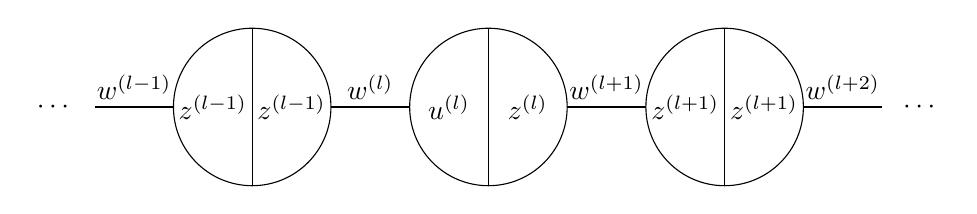
\begin{tikzpicture}[scale=1]
      \draw (-5,0) -- (5,0);
      \draw (5.5,0) node{$\cdots$};
      \draw (-5.5,0) node{$\cdots$};
      \filldraw[fill=white] (-3,0) circle[radius=1];
      \filldraw[fill=white] (0,0) circle[radius=1];
      \filldraw[fill=white] (3,0) circle[radius=1];
      \draw (-0.5,0) node{$u^{(l)}$}; 
      \draw (0.5,0) node{$z^{(l)}$}; 
      \draw (2.5,0) node{$z^{(l+1)}$}; 
      \draw (3.5,0) node{$z^{(l+1)}$}; 
      \draw (-2.5,0) node{$z^{(l-1)}$}; 
      \draw (-3.5,0) node{$z^{(l-1)}$}; 
      \draw (-4.5,0.25) node{$w^{(l-1)}$};
      \draw (-1.5,0.25) node{$w^{(l)}$};
      \draw (1.5,0.25) node{$w^{(l+1)}$};
      \draw (4.5,0.25) node{$w^{(l+2)}$};
      \draw (-3,-1) -- (-3,1);
      \draw (0,-1) -- (0,1);
      \draw (3,-1) -- (3,1);
    \end{tikzpicture}
    \caption{1つのユニットからなる層を1列につなげたニューラルネットワークの第$l$層に注目した図}
    \label{チェインニューラルネットワーク}
  \end{center}
\end{figure}
この場合,第$l$層の活性は$u^{(l)} = w^{(l)} z^{(l-1)} = w^{(l)}  f(u^{(l-1)})$で出力が$\hat{y} = z^{(L)} = f(u^{(L)})$であることから,
\begin{align}
  y
  &= f(u^{(L)}) \notag \\
  &= w^{(L)} f\left(u^{(L-1)} \right) \notag \\
  &= w^{(L)} f\left(w^{(L-1)} f\left(u^{(L-2)} \right) \right) \notag \\
  & \qquad \vdots \notag \\
  &= f\left( w^{(L)} f\left(w^{(L-1)} f\left( \cdots w^{(l+1)} f\left(w^{(l)} f\left(\cdots f(x)\right)\right)\right)\right)\right)
\end{align}
となり,これは多数の写像の合成になっているということがわかる.したがって,これを$w^{(l)}$で微分しようと思う場合,最終の第$L$層から離れれば離れるほど巨大な合成関数を計算して,その微分を実行することになる.このように多層ニューラルネットワークのパラメータ微分は層の深さが原因で計算が複雑になってしまう.計算の複雑さのほかにも,そのまま安直に数値微分として実装するのは精度としても計算量の観点からしても良い方法ではない.ではどうするかというと,我々の手で簡略化できるところは数学的に計算し尽くして,シンプルなアルゴリズムの形に帰着させてから実装するのである.その結果から得られるアルゴリズムが誤差逆伝播法というスマートな手法である\par
誤差逆伝播法の仕組みを理解するため,まず$u^{(l)} = w^{(l)} z^{(l-1)}$という関係に注目する.$w^{(l)}$の変動はまずは$u^{(l)}$の値に直接影響を与えるため,チェインルールより
\begin{equation}
  \frac{\partial E}{\partial w^{(l)}}
  = \frac{\partial E}{\partial u^{(l)}} \frac{\partial u^{(l)}}{\partial w^{(l)}}
  = \frac{\partial E}{\partial u^{(l)}} z^{(l-1)}
  \equiv \delta^{(l)} z^{(l-1)}
\end{equation}
と書き換えられる.したがって$\delta^{(l)} \equiv \partial E / \partial u^{(l)}$という量がわかれば勾配が決まる.ところが$u^{(l+1)} = w^{(l+1)} f(u^{(l)})$であるため,このデルタが次の層の$\delta^{(l+1)}$と関係付く.つまり,
\begin{align}
  \delta^{(l)}
  &= \frac{\partial E}{\partial u^{(l+1)}} \frac{\partial u^{(l+1)}}{\partial u^{(l)}}
  = \delta^{(l+1)} w^{(l+1)} f'(u^{(l)}) \notag \\
  \delta^{(l+1)}
  &= \frac{\partial E}{\partial u^{(l+2)}} \frac{\partial u^{(l+2)}}{\partial u^{(l+1)}}
  = \delta^{(l+2)} w^{(l+2)} f'(u^{(l+1)}) \notag \\
  & \qquad \vdots \notag \\
  \delta^{(L-1)}
  &= \frac{\partial E}{\partial u^{(L)}} \frac{\partial u^{(L)}}{\partial u^{(L-1)}}
  = \delta^{(L)} w^{(L)} f'(u^{(L)}) \notag \\
  \delta^{(L)}
  &= \frac{\partial E}{\partial u^{(L)}}
\end{align}
である.したがって$\delta^{(L)}$から順に遡って$\delta$の値を計算していけば,誤差関数のパラメータ微分を計算することができる.これが誤差逆伝播法の考えである.

\subsection{誤差関数の勾配計算}
\begin{figure}[H]
  \begin{center}
    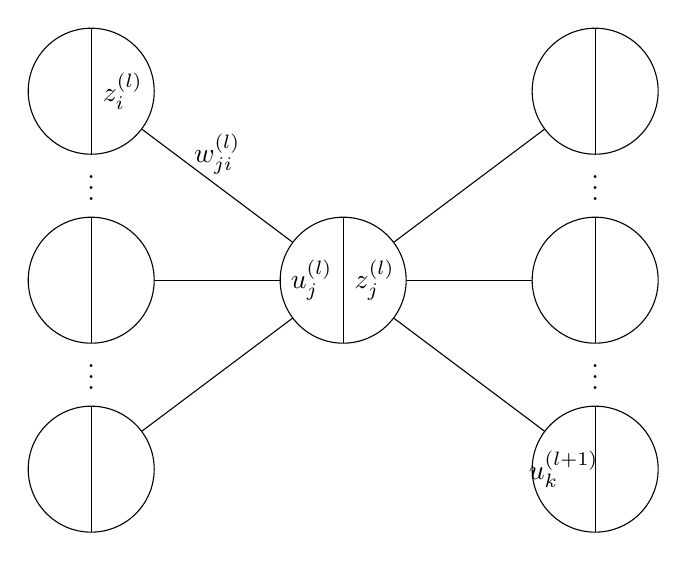
\begin{tikzpicture}[scale=0.8]
      \draw (-3,0) -- (3,0);
      \draw (-4,3) -- (4,-3);
      \draw (-4,-3) -- (4,3);
      \filldraw[fill=white] (-4,3) circle[radius=1];
      \filldraw[fill=white] (-4,0) circle[radius=1];
      \filldraw[fill=white] (-4,-3) circle[radius=1];
      \filldraw[fill=white] (0,0) circle[radius=1];
      \filldraw[fill=white] (4,3) circle[radius=1];
      \filldraw[fill=white] (4,0) circle[radius=1];
      \filldraw[fill=white] (4,-3) circle[radius=1];
      \draw (-0.5,0) node{$u_j^{(l)}$}; 
      \draw (0.5,0) node{$z_j^{(l)}$}; 
      \draw (-3.5,3) node{$z_i^{(l)}$}; 
      \draw (3.5,-3) node{$u_k^{(l+1)}$}; 
      \draw (-2,2) node{$w_{ji}^{(l)}$}; 
      \draw (-4,1.6) node{$\vdots$}; 
      \draw (-4,-1.4) node{$\vdots$}; 
      \draw (4,1.6) node{$\vdots$}; 
      \draw (4,-1.4) node{$\vdots$}; 
      \draw (0,-1) -- (0,1);
      \draw (-4,4) -- (-4,2);
      \draw (-4,1) -- (-4,-1);
      \draw (-4,-2) -- (-4,-4);
      \draw (4,4) -- (4,2);
      \draw (4,1) -- (4,-1);
      \draw (4,-2) -- (4,-4);
    \end{tikzpicture}
    \caption{1つのユニットからなる層を1列につなげたニューラルネットワークの第$l$層に注目した図}
    \label{誤差逆伝播法の例}
  \end{center}
\end{figure}

誤差逆伝播法に至るためのアイデアの1つ目は,巨大な合成関数の微分を一挙に計算せず,困難を分割することであった.そのために注目している重み$w_{ji}^{(l)}$の変動が,ネットワークの局所的な構造を通じて周囲にどれくらいの影響を与えるか,という観点から勾配を書き換える.図\ref{誤差逆伝播法の例}のように,重み$w_{ji}^{(l)}$の変動は,まず$l$のユニット$j$の総入力を変化させる.この総入力$u_j^{(l)}$の変動がネットワークを順次伝播していき,出力を変化させ,最終的に誤差関数の変動を与える.この事実を微分操作で表現すると,誤差関数$E_n(u_j^{(l)}(w_{ji}^{(l)}))$は総入力$u_j^{(l)}$を通じて,重み$w_{ji}^{(l)}$に間接的に依存しているため,
\begin{equation}
  \frac{\partial E_n}{\partial w_{ji}^{(l)}}
  = \frac{\partial E_n}{\partial u_j^{(l)}} \frac{\partial u_j^{(l)}}{\partial w_{ji}^{(l)}} \notag \\
  = \delta_j^{(l)} z_i^{(l-1)} \label{ニューラルネットワークパラメータ微分}
\end{equation}
と書くことができる.2行目の右辺の1つ目の因子をデルタとよび.
\begin{equation}
  \delta_j^{(l)}
  \equiv \frac{\partial E_n}{\partial u_j^{(l)}}
\end{equation}
と定義した.これはユニット$j$からのシグナルが,どれほど最終的に誤差に聞いているかを測る尺度となる量である.したがって,この値が求まれば勾配が決定する.このように勾配をデルタとユニット出力に分けることが第1ステップである.\par
第2ステップであるデルタを決めるアルゴリズムは誤差逆伝播法の核となる部分である.実はこの部分も,答えが一度わかってしまえばそれほど難しい話ではない.なぜなら,デルタを満たす漸化式を見つけてやればよいからである.漸化式を導くのみ,デルタの定義に立ち返ってみる.デルタは誤差関数をユニット$j$への総入力$u_j^{(l)}$で微分したものである.そこでこの総入力の変化がどのように誤差関数に影響をするのかを見るために,再びネットワークの局所的な構造に注目する.図\ref{誤差逆伝播法の例}より,ユニット$j$の総入力$u_j^{(l)}$は活性化関数が作用することでこのユニットの出力へ変換され,隣接する$l+1$層のユニットたちへ入力する.したがって$u_j^{(l)}$の変動は,次層のユニットたちの総入力$u_k^{(l+1)}$の変化を通じて誤差関数を変動させる.つまり微分係数は
\begin{equation}
  \delta_j^{(l)}
  = \frac{\partial E_n}{\partial u_j^{(l)}}
  = \sum_{k=0}^{d_{l+1}-1} \frac{\partial E_n}{\partial u_k^{(l+1)}}\frac{\partial u_k^{(l+1)}}{\partial u_j^{(l)}}
\end{equation}
という性質を満たす.右辺の1つ目の因子は$l+1$層でのデルタ$\delta_k^{(l+1)}$にほかならないため,この式は隣接層間のデルタの間の漸化式である.
\begin{equation}
  u_k^{(l+1)}
  = \sum_{j'} w_{kj'}^{(l+1)} f(u_{j'}^{(l)})
\end{equation}
であったことを思い出すと,この式は次のようにまとめることができる.
\begin{equation}
  \delta_j^{(l)}
  = \sum_{k=0}^{d_{l+1}-1} \delta_k^{(l+1)} w_{kj}^{(l+1)} f'(u_{j'}^{(l)})
\end{equation}
これがデルタの逆伝播を記述する式である.逆伝播とよばれる理由は,通常のニューラルネットワークの入力が
\begin{equation}
  u_j^{(l)}
  = \sum_{k=0}^{d_{l+1}-1} w_{kj}^{(l)} f(u_{i'}^{(l-1)}) \label{デルタ逆伝播}
\end{equation}
を通じて重み$w_{ji}^{(l)}$と活性化関数$f$を受け取りながら$l-1$層から$l$層へ順伝播するのに対し,式\ref{デルタ逆伝播}を見ると,デルタという量が$w_{kj}^{(l+1)}$倍の作用を受けて$l+1$層から$l$層へ逆向きに伝播しているからである.実際にデルタを計算するアルゴリズムにおいても,出力層で計算されたデルタの「初期値」の情報を入力層側に向けて順次逆向きに伝播させている.したがって,実際の計算では,まず入力を出力層まで順伝播させ,出力層での誤差を計算させる.そして,その結果をもとにデルタを逆伝播させる.
\begin{align}
  &\bm{x}_n = \bm{z}^{(1)} \rightarrow \bm{z}^{(2)} \rightarrow \cdots \rightarrow \bm{z}^{(L-1)} \rightarrow \bm{z}^{(L)} = \hat{\bm{y}} \notag\\
  &\bm{\delta}^{(1)} \leftarrow \bm{\delta}^{(2)} \leftarrow \cdots \leftarrow \bm{\delta}^{(L-2)} \leftarrow \bm{\delta}^{(L-1)} \leftarrow \bm{\delta}^{(L)}
\end{align}
$\bm{\delta}^{(l)}$は$l$層のデルタを並べて作ったベクトルである.来れたの結果を式\ref{ニューラルネットワークパラメータ微分}の形に組み合わせることですべての勾配が決まる.
\begin{equation}
  \frac{\partial E_n}{\partial \bm{w}_{ji}^{(l)}}
  = \bm{\delta}^{(l)} \left( \bm{z}^{(l-1)} \right)^{\top}
\end{equation}
これが誤差逆伝播法である.

\subsection{逆伝播計算の初期値}
逆伝播において漸化式を解くための初期値にあたるのは,出力層におけるデルタである.この値は簡単に計算できる.というのも出力層の活性化関数を$f$とすると,最終出力は$\hat{y}_j=f(u_j^{(L)})$であるため,出力層のユニット$j$のデルタは$E_n(\hat{y}_j(u_j^{(L)}))$を$u_j^{(L)}$で微分して,
\begin{equation}
  \delta_j^{(L)}
  = \frac{\partial E_n}{\partial \hat{y}_j} f'(u_j^{(L)})
\end{equation}
となるからである.例えば回帰問題などの場合には誤差関数として二乗誤差$E_n=(\hat{\bm{y}}(\bm{x};\bm{w})-\bm{y})^2/2$が用いられる.この場合デルタの具体形は
\begin{equation}
  \delta_j^{(L)} = (\bm{y}_j - y_j)\hat{y}'_j (u_j^{(L)})
\end{equation}
である.出力層の活性化関数が恒等写像であれば,当然ながら$\delta_j^{(L)}=(\hat{y}_j-y_j)$であり,前節のデルタ則のパラメータ更新(\ref{現代パーセプトロンの学習則})を再現する.\par
一方,誤差関数が交差エントロピー(\ref{ソフトマックス交差エントロピー})である場合,
\begin{equation}
  \delta_j^{(L)}
  = -\sum_k \frac{t(y_n)_k}{\hat{y}_k}\hat{y}'_k(u_j^{(L)})
\end{equation}
であった.この出力層の活性化関数はソフトマックス$y_k = e^{u_k^{(L)}}/\sum_{k'}e^{u_{k'}^{(L)}}$である.ソフトマックスの微分はクロネッカーのデルタを用いると
\begin{equation}
  \frac{\partial \hat{y}_k}{\partial u_j^{(L)}}
  = \delta_{kj} \hat{y_k} - \hat{y}_j \hat{y}_k
\end{equation}
と書き換えられるという性質がある.さらにクラス分類のときは,どのような訓練サンプルも$\sum_kt_k=1$という性質を満たしているため,デルタは結局$\delta_j^{(L)}=(\hat{y}_j - t_j)$という先ほどと同じ形に帰着する.

\subsection{勾配計算}
勾配計算の目的はニューラルネットワークの勾配法による学習であったので,誤差逆伝播で終わりではない.各訓練サンプルに対して計算された勾配$\partial E_n/\partial w_{ji}^{(l)}$を,学習に用いる(ミニ)バッチ$\mathcal{D}$で平均して実際のパラメータの更新量を求める必要がある.
\begin{equation}
  \Delta w_{ji}^{(l)}
  = -\eta \frac{\partial E}{\partial w_{ji}^{(l)}}
  = -\eta \frac{1}{|\mathcal{D}|} \sum_{n \in \mathcal{D}}\frac{\partial E}{\partial w_{ji}^{(l)}}
\end{equation}
そのうえで,各時刻$t$でのパラメータ値で計算した$\Delta w_{ji}^{(t,l)}$を使って
\begin{equation}
  w_{ji}^{(t+1,l)}
  = w_{ji}^{(t,l)} + \Delta w_{ji}^{(t,l)}
\end{equation}
と重みパラメータを更新する.その後再び順伝播と逆伝播を行い,次時刻にも同じ操作を繰り返す.これをパラメータの収束まで繰り返すのが勾配降下法による学習であった.

\subsection{デルタの意味}
ここでは誤差逆伝播法に現れたデルタの意味について説明する.出力層におけるデルタには$\delta_j^{(L)}=\hat{y}_j(\bm{x};\bm{w})-y_j$という形をしていた.これは訓練サンプル$\bm{x}$を入力した際の最終出力$\bm{y}$と,訓練サンプルの目標信号$\bm{y}$の差なので,まさにニューラルネットワークによる推論の誤差である.勾配降下法はこの誤差をできるだけ打ち消すように,出力層とその手前の層の間の重みパラメータ$w_{pq}^{(L)}$を修正する.つまり,このデルタ$\bm{\delta}^{(L)}$は,出力層ノードにつながる重みがどの程度誤差に寄与しているかを測る量になっている.では,中間層のノードたちがどのくらい誤差関数に効いているかを測っているのでしょうか.\par
中間層のノードの総入力を
\begin{equation}
  u_j^{(l)} \rightarrow u_j^{(l)} + \Delta u_j^{(l)}
\end{equation}
と変動させてみる.デルタの定義から,この変動により誤差関数はだいたい
\begin{equation}
  \Delta E \approx \delta_j^{(l)} \Delta u_j^{(l)}
\end{equation}
だけズレる.もしこのデルタ係数がほとんど0に近ければ,このノードの総入力の大きさを調整してもほとんど誤差関数の大きさは改善できないことになる.つまりこのノードへの総入力を決めている重みたちは,ほとんど誤差に寄与しないということになる.\par
一方デルタの絶対値が大きい場合は,このノードの総入力を変えることで誤差関数は劇的に変動する.つまり,パラメータ空間の中で,現在地点から少しずれるだけで大きく誤差関数が変化しえるため,現在のニューラルネットワークは最適値よりかなり上にいる可能性があるといえる.つまりこのノードの総入力は,誤差関数を極小化しない不適切な値を示しているということであるため,誤差を減らすようにこのノードへの入力重み$w_{ji}^{(l)}$を修正すべきである.この総入力の変動と逆符号の方向に変動を与えるパラメータの修正をする.これが誤差逆伝播法をもとにした勾配降下法を行っていることにほかならない.このように一般化デルタ$\delta_j^(l)$は,$l$層のノード$j$に付随した局所的な誤差を測る量になっている.






\chapter{機械学習によるイジング模型の相転移検出}
この章では,機械学習,特にニューラルネットワークを用いたイジング模型の磁気相転移温度の検出に関する研究について述べる.\par
相転移を機械学習で捉えることができるかという問題は,カラスクイラ(Juan Carrasquilla)とメルコ―(Roger G.Melko)によって議論され,2016年5月に実際にうまくいくということを示した.彼らは,イジングスピン配位を入力したときに,その配位が強磁性相と常磁性相のどちらに属するかを分類するモデルをニューラルネットワークを用いて構築し,それを配位データとどちらの相に属しているかを与える教師ラベルの教師ありデータセットを用いて教師あり学習を行い,相の分類器を作成した.\par
この研究は,ニューラルネットワークが相転移温度を見分けることができるということ示す大きな発見であった.ただし,学習データするのに相転移の情報が必要であるため,相転移温度が未知の系に対して応用するのは難しいという,汎用性に問題があった.\par
そんな中,2017年6月に富谷昭夫と田中章詞は,教師データに相転移ラベルではなく,温度ラベルを用いて教師あり学習を行って,入力された配位データから,その配位の温度を測定する温度測定器を作成し,作成した温度測定器の重みパラメータから相転移温度を高い精度で予測できることを示した.これは,学習データに相転移温度に関する情報は全く含まれていないため,モデルが配位と温度のみから,相転移温度を学習できることを示しており.カラスクイラとメルコーによる研究の問題点である汎用性を改善する結果となった.\par
また,なぜニューラルネットワークが相転移温度の情報を学習できるのかという研究が2019年に柏浩二,菊池勇太,富谷昭夫によってニューラルネットワークによる学習の仕組みの理論的な部分まで理解された.
\section{イジング模型のモンテカルロ法}
相転移検出に関する研究の前に,学習に用いるためのデータセットをどのようにして生成するかを説明する必要がある.ここでは,モンテカルロ法を用いて,イジング模型による機械学習で必要な学習データをどのようにして生成するのかについて説明する.\par
モンテカルロ法とは乱数を使って積分や和を行う手法である.ここでは,期待値の和を乱数を用いて調べる.表記の都合上,今後スピン配位を$C(=\{\bm{\sigma}\})$と表記することにする.あるスピン配位$C$の実現確率を
\begin{equation}
  \label{スピン配位の実現確率}
  P(C)=\frac{1}{Z}e^{-\beta E[C]}
\end{equation}
として確率的にスピン配位$C$を生成して,生成したスピン配位$C$を使った平均を用いて期待値を推定する手法をとる.\par
しかし,スピン配位$C$の実現確率(\ref{スピン配位の実現確率})は直接計算できない.なぜなら,分母の分配関数$Z$を計算するために,結局全ての配位の和を計算する必要があるからである.そこで,分配関数$Z$の計算を避けてスピン配位を生成できる手法であるマルコフ連鎖モンテカルロ法(Markov chain Monte-Carlo)を以下で説明する.

\subsection{マルコフ連鎖モンテカルロ法}
今,調べたい期待値は一般的に
\begin{equation}
  \mathbb{E}[f(C)] = \sum_{C} f(C)P(C)
\end{equation}
と書ける.ここで$f(C)$は配位の関数で,例えば磁化率などである.また,$\sum_{C}$は可能なスピン配位についての足し上げを表す.格子点の数が$K$個であるとき,イジング模型なら$2^K$個の足し算になる.これを
\begin{equation}
  \mathcal{C} = \{ C_1, C_2, C_3, \cdots \}
\end{equation}
という$2^K$よりもずっと短い列の平均に置き換え,
\begin{equation}
  \mathbb{E}[f(C)] \approx \frac{1}{|\mathcal{C|}}\sum_{C_k \in \mathcal{C}}f(C_k)
\end{equation}
を代わりに評価したい.ここで$|\mathcal{C}|$は配位の数を表す.当然,適当に作った列では正しい期待値を与えないが,以下を満たす$P(C_a|C_b)$に従って$C$を生成すれば正しい期待値を与えることが知られている.
\begin{equation}
  P(C_a|C_b)P(C_b) = P(C_b|C_a)P(C_a)
\end{equation}
これは大数の法則を用いることで証明することができる.ここで条件付き確率$P(C_a|C_b)$は遷移確率とよばれ,この式は詳細釣り合い(detailed balance)の式と呼ばれている.乱数を使ったアルゴリズムをモンテカルロ法と呼ぶが,上のような確率的に配位の列を作るアルゴリズムをマルコフ連鎖モンテカルロ法という.\par

\subsection{イジング模型に対するメトロポリス法}
マルコフ連鎖モンテカルロ法にもいくつかの手法が存在し,その中でとくによく用いられているものとして,メトロポリス法と熱浴法があげられる.ここではメトロポリス法について説明する.\par
ある配位$C_b$と$C_a$を比較したときに$C_a$のエネルギーの方が低い場合,つまり$E(C_b)>E(C_a)$を考える.この場合は$C_a$の方がエネルギー的に安定なので,$C_b$から$C_a$への遷移確率を
\begin{equation}
  P(C_a|C_b) = 1
\end{equation}
ととることにする.このとき,詳細釣り合いの式は
\begin{equation}
  P(C_b) = P(C_b|C_a)P(C_a)
\end{equation}
となる.これより,$C_a$から$C_b$の遷移確率が決まってしまい,
\begin{equation}
  P(C_b|C_a) = \frac{P(C_b)}{P(C_a)} = \frac{e^{-\beta E(C_b)}/Z}{e^{-\beta E(C_a)}/Z} = e^{ -\beta\Big( E(C_b)-E(C_a) \Big)}
\end{equation}
となる.したがって,$C_a$から$C_b$の遷移確率として,
\begin{equation}
  P(C_b|C_a)=
  \begin{cases}
    \exp\Big[ -\beta\Big( E(C_b)-E(C_a) \Big) \Big], & E(C_b)>E(C_a) \\
    1,                                               & E(C_b)<E(C_a)
  \end{cases}
\end{equation}
ととると詳細釣り合いの式を満たすことになる.このアルゴリズムをメトロポリス法と呼ぶ.\par
メトロポリス法をイジング模型に適用する場合の手順をまとめる.
\begin{enumerate}
  \item 適当な配位$C_1$を用意する.
  \item 以下を$i = 1,2,3,\cdots,N_{\text{conf}}$まで繰り返す,
        \begin{enumerate}
          \item $C_i$のあるサイトのスピンを反転し,その配位を$C'_i$とおく.
          \item エネルギー$E(C_i)$と$E(C'_i)$を計算する.
          \item $E(C_i)>E(C'_i)$なら$C_{i+1}=C'_i$とし,$i \rightarrow i+1$とおいて(a)へ戻る.(受理(accept))
          \item 乱数$r \in [0,1]$を用意し,$\Delta E = E(C'_i)-E(C_i)$に対して,$r < \exp(-\beta\Delta E)$ならば$C_{i+1}=C'_i$とし,$i \rightarrow i+1$とおいて(a)へ戻る.(受理(accept))
          \item $C_{i+1}=C_i$とし,$i \rightarrow i+1$とおいて(a)へ戻る.(棄却(reject))
        \end{enumerate}
\end{enumerate}
ここで,「棄却」は提案された配位を使わずに前の配位をそのまま次の配位として受け入れるという意味であることに注意が必要である.\par
上記の手順に従うと,配位の列
\begin{equation}
  \mathcal{C} = \{ C_1,C_2,C_3,\cdots,C_{N_{\text{conf}}} \}
\end{equation}
が得られる.しかし最初の方の配位は適当に選んだ初期配位の影響を受けているため,期待値の計算に含めてはいけない.例えば$N_{\text{disc}}(1<N_{\text{disc}}<<N_{\text{conf}})$番目(discはdiscardの略)まで除いたとすると,
\begin{equation}
  \mathbb{E}[f(C)] \approx \frac{1}{N_{\text{disc}} - N_{\text{conf}}}\sum_{k=N_{\text{disc}}}^{N_{\text{conf}}}f(C_k)
\end{equation}
のように期待値を計算できる.$N_{\text{disc}}$は配位ごとの物理量を観察して初期配位の影響がなくなったあたりの番号をとればよい.

\subsection{イジング模型の熱浴法}
次に熱浴法(heatbath algorothm)をみる.このアルゴリズムは機械学習の文脈ではギブスサンプリング(Gibbs sampling)と呼ばれる.熱浴法は,ある1自由度を着目し,その周りの自由度を熱浴とみなして更新するマルコフ連鎖モンテカルロ法の一種である.\par
熱浴法は条件付き確率から導出される.イジング模型のあるサイト$j$に着目し,そのサイト以外を熱浴をみなしたときにサイト$j$がどうなるかを条件付き確率に従って決めるのである.\par
例えば,
\begin{align}
   & C_j \text{:サイト$j$にあるスピンの状態} \\
   & \overline{C}_j \text{:サイト$j$以外のスピンの状態}
\end{align}
とすると,$\overline{C}_j$の下での$C_j$の条件付き確率は
\begin{equation}
  P(C_j|\overline{C}_j) = \frac{P(C_j,\overline{C}_j)}{P(\overline{C}_j)}
\end{equation}
と書ける.ある配位を与える確率を
\begin{align}
  P(C) &= P(C_j,\overline{C}_j) \notag \\
  &= \frac{1}{Z}\exp{\left[ -\beta J \sigma_j \sum_{k\in \mathcal{N}(j)} \sigma_k + (\sigma_j\text{を含まない項}) \right]}
\end{align}
と書く.ここで,サイト$j$の最近接サイトをまとめて$\mathcal{N}(j)$と書いた.\par
$C_j$の状態(サイト$j$のスピン状態)を足し上げて周辺化した確率$P(\overline{C}_j)$は,$P(\overline{C}_j)=\sum_{C_j}P(C_j,\overline{C}_j)$を使うと$A_j$は$\sigma_j=\{+1,-1\}$をとるので,全て足し上げて
\begin{equation}
  P(\overline{C}_j) = \frac{1}{Z}\sum_{\sigma_j=\pm 1}\exp{\left[ -\beta J \sigma_j \sum_{k\in \mathcal{N}(j)} \sigma_k + (\sigma_j\text{を含まない項}) \right]}
\end{equation}
とわかる.ここから条件付き確率$P(C_j|\overline{C}_j)$は,定義$P(C_j|\overline{C}_j)=P(C_j,\overline{C}_j)/P(\overline{C}_j)$から
\begin{align}
  P(C_j|\overline{C}_j)
   & = \frac{1}{Z}\exp{\left[ -\beta J \sigma_j \sum_{k\in \mathcal{N}(j)} \sigma_k + (\sigma_j\text{を含まない項}) \right]} \Bigg/                                                                                                      \notag            \\
   & \hspace{0.5cm} \frac{1}{Z}\sum_{\sigma_j=\pm 1}\exp{\left[ -\beta J \sigma_j \sum_{k\in \mathcal{N}(j)} \sigma_k + (\sigma_j\text{を含まない項}) \right]}                                                                                           \notag \\
   & = \frac{\exp{\left[ -\beta J \sigma_j \sum_{k\in \mathcal{N}(j)} \sigma_k\right]}}{\sum_{\sigma_j=\pm 1}\exp{\left[ -\beta J \sigma_j \sum_{k\in \mathcal{N}(j)} \sigma_k \right]}}                                             \notag                    \\
   & = \frac{\exp{\left[ -\beta J \sigma_j \sum_{k\in \mathcal{N}(j)} \sigma_k\right]}}{\exp{\left[ -\beta J \sum_{k\in \mathcal{N}(j)} \sigma_k \right]} + \exp{\left[ +\beta J \sum_{k\in \mathcal{N}(j)} \sigma_k \right]}}
\end{align}
となる.最後の式を見ると,サイト$j$の周りのスピン配位だけでサイト$j$の状態が決まるということがわかる.また,ここでもメトロポリス法のときと同様に分配関数$Z$の計算が必要なくなっている.\par
例えば,サイト$j$のスピンが$+1$である場合は
\begin{equation}
  P(s_j = +1)
  = \frac{\exp{\left[\beta J \sum_{k \in \mathcal{N}(j)}s_k\right]}}{\exp{\left[\beta J \sum_{k \in \mathcal{N}(j)}s_k\right]} + \exp{\left[-\beta J \sum_{k \in \mathcal{N}(j)}s_k\right]}}
\end{equation}
となる.なのでこの確率に従って次の配位におけるサイト$j$のスピンを決定(更新)すればよい.この確率の評価はメトロポリス法の乱数を使っている個所と同じように乱数を用いて評価すればよい.また$P(s_j = -1|B) = 1 - P(s_j =+1|B)$である.そして空間全部のスピンについて繰り返せば次の配位が得られる.



\section{相の分類器による相転移検出}
ここから,相の分類器によるイジング模型の磁気相転移の検出について説明する.カラスクイラとメルコ―は,2016年の5月に"Machine learning phases of matter"を投稿し,後にNature Physics誌に掲載された.彼らの研究によってはじめてニューラルネットワークを用いて相転移が検出可能であることが示された.ここでは相の分類を行うこの学習済みモデルを相の分類器とよぶことにする.以下では,2次元正方イジング模型の相の分類器の作成についての説明と,作成した2次元正方イジング模型の相の分類器が2次元三角イジング模型の相分類にそのまま適用できることを説明する.\par
\subsection{データセットの作成}
ニューラルネットワークを用いて学習を行うためのデータセットの作成についてここで述べる.相分類器の作成には,スピン配位のデータとその配位が強磁性相か常磁性相かを示す教師ラベルをセットにした教師ありデータを大量に用意する必要がある.\par
この教師データの作成は次の手順で作成した.
\begin{enumerate}
  \item 逆温度ラベル$\beta_i, \ i=1,2,\dots,N_{\text{label}}$を設定する.
  \item 以下を$i=1,2,\dots,N_{\text{label}}$まで繰り返す.
  \begin{enumerate}
    \item メトロポリス法を用いて逆温度$\beta_i$のスピン配位$\bm{\sigma}$を$N$個サンプルする
    \item $\beta_i<\beta_{\text{cr}}$の場合$d=0$(常磁性相),$\beta<\beta_{\text{cr}}$の場合$d=0$(強磁性相)とする
    \item $(\bm{\sigma},d)$とする.
  \end{enumerate}
\end{enumerate}
このような手順で作成したスピン配位の例が図\ref{相の分類器データセット}である.
\begin{figure}[H]
   \begin{center}
       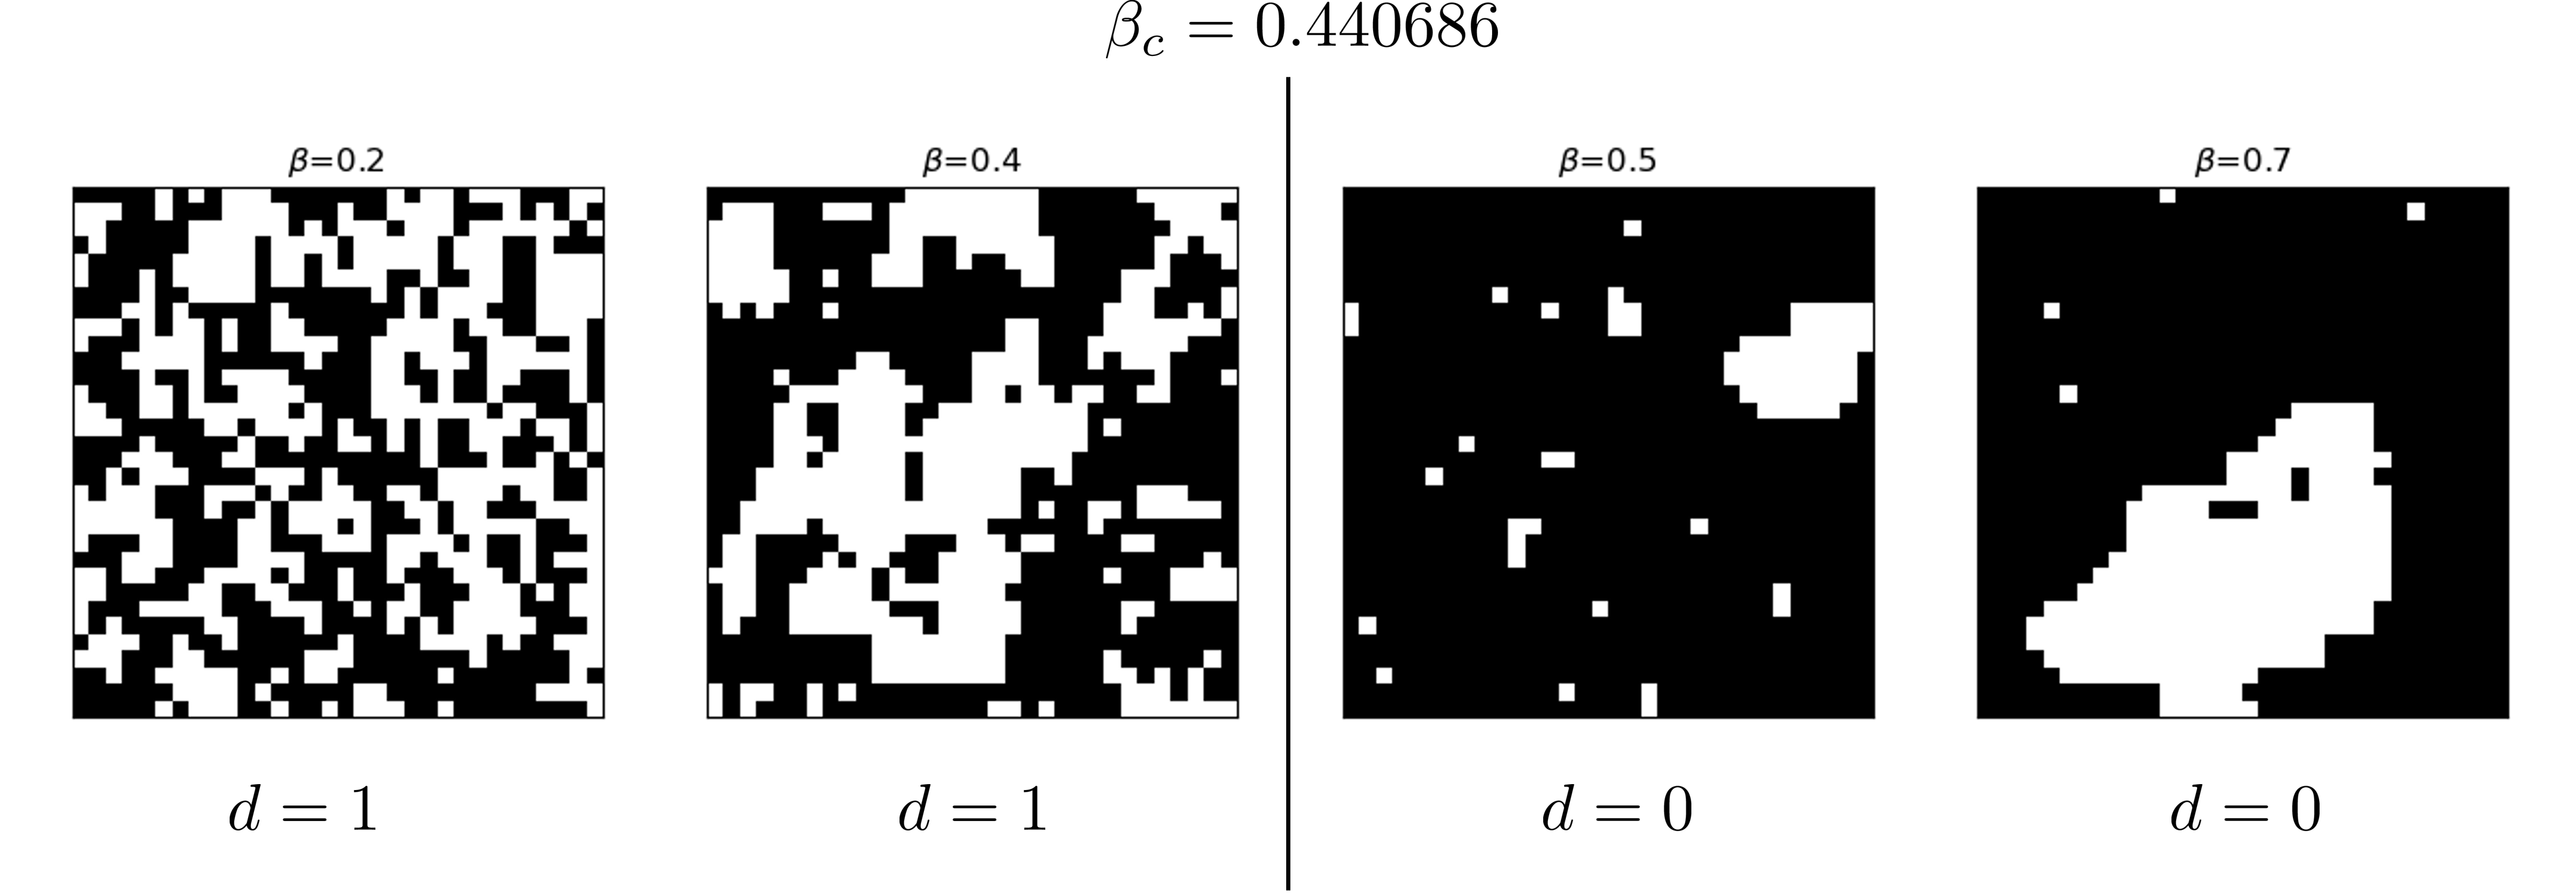
\includegraphics[width=\linewidth]{image/配位ラベルと相転移ラベル.png}
       \caption{2次元正方イジング模型のサンプルデータの例}
       \label{相の分類器データセット}
   \end{center}
\end{figure}
$\beta=0.4$と$\beta=0.5$でスピンの揃い具合に大きく違いが表れているのが見てとれる.これは2つの温度間2次元正方イジング模型の相転移点$\beta_c = 0.44086$が存在するからである.理論的にはこの温度より高いとき(逆温度の値が小さいとき)スピンはバラバラになり,低いとき(逆温度の値が大きいとき)スピンは揃う.\par
今回は,次のように相転移点周りの20個の逆温度ラベル設定した.
\begin{align*}
  \{\beta_i\} 
  = \{ &0.00,0.05,0.10,0.15,0.20,0.25,0.30,0.35,0.40,0.42,\\
  &0.47,0.5,0.55,0.60,0.65,0.70,0.75,0.80,0.85,0.90 \}
\end{align*}
そして,格子サイズを$32 \times 32$としメトロポリス法を用いて各ラベルに対して,90個のスピン配位をサンプルした.つまり全データ数は1800になる.\par
\subsubsection*{三角イジング模型}
また,三角イジング模型に対しても同様な方法でデータを生成した.ただし,三角イジング模型の相転移逆温度は$\beta \sim 0.2746$なので以下の20個の逆温度ラベルを用いた.
\begin{align*}
  \{\beta_i^{\text{tri}}\} 
  = \{ &0.00,0.03,0.06,0.09,0.12,0.15,0.18,0.21,0.23,0.25,\\
  &0.29,0.31,0.33,0.36,0.39,0.42,0.45,0.48,0.51,0.54 \}
\end{align*}

\subsection{モデルの構築と学習}
前の節でデータセットの作成手順を説明したので次にデータセットを学習させるモデルを説明する.ここでは,2種類のニューラルネットワークを用いて学習を行った.1つ目は全結合層のみからなるニューラルネットワーク(以後,FCNモデルとよぶ).2つ目は畳み込み層を加えたニューラルネットワーク(以後,CNNモデルとよぶ)である.\par
まず,FCNモデルに構造ついて説明する.次のような順伝播を行うモデルで実験を行った.
\begin{equation}
  \left[
    \begin{aligned}
      & \mathcal{I} = \left\{ \{ \sigma_i \} \Big| \ \text{Ising configs on} \ L \times L \ \text{lattice.} \right\} \\
       & \downarrow
      \begin{cases}
        \text{Flatten} \\
        \text{Fully-connected layer} \\
        \text{ReLU activation}
      \end{cases} \\
       & x_i \in \mathbb{R}^{N_h} \ \text{: hidden units} \\
       & \downarrow
      \begin{cases}
        \text{Fully-connected layer} \\
        \text{Softmax activation}
      \end{cases} \\
       & y_K \in [0,1]^{2} \ \text{: output units}
    \end{aligned}
    \right]
\end{equation}
また,図$\ref{相分類FCNモデル}$はFCNモデル概要図である.

\begin{figure}[H]
  \begin{center}
    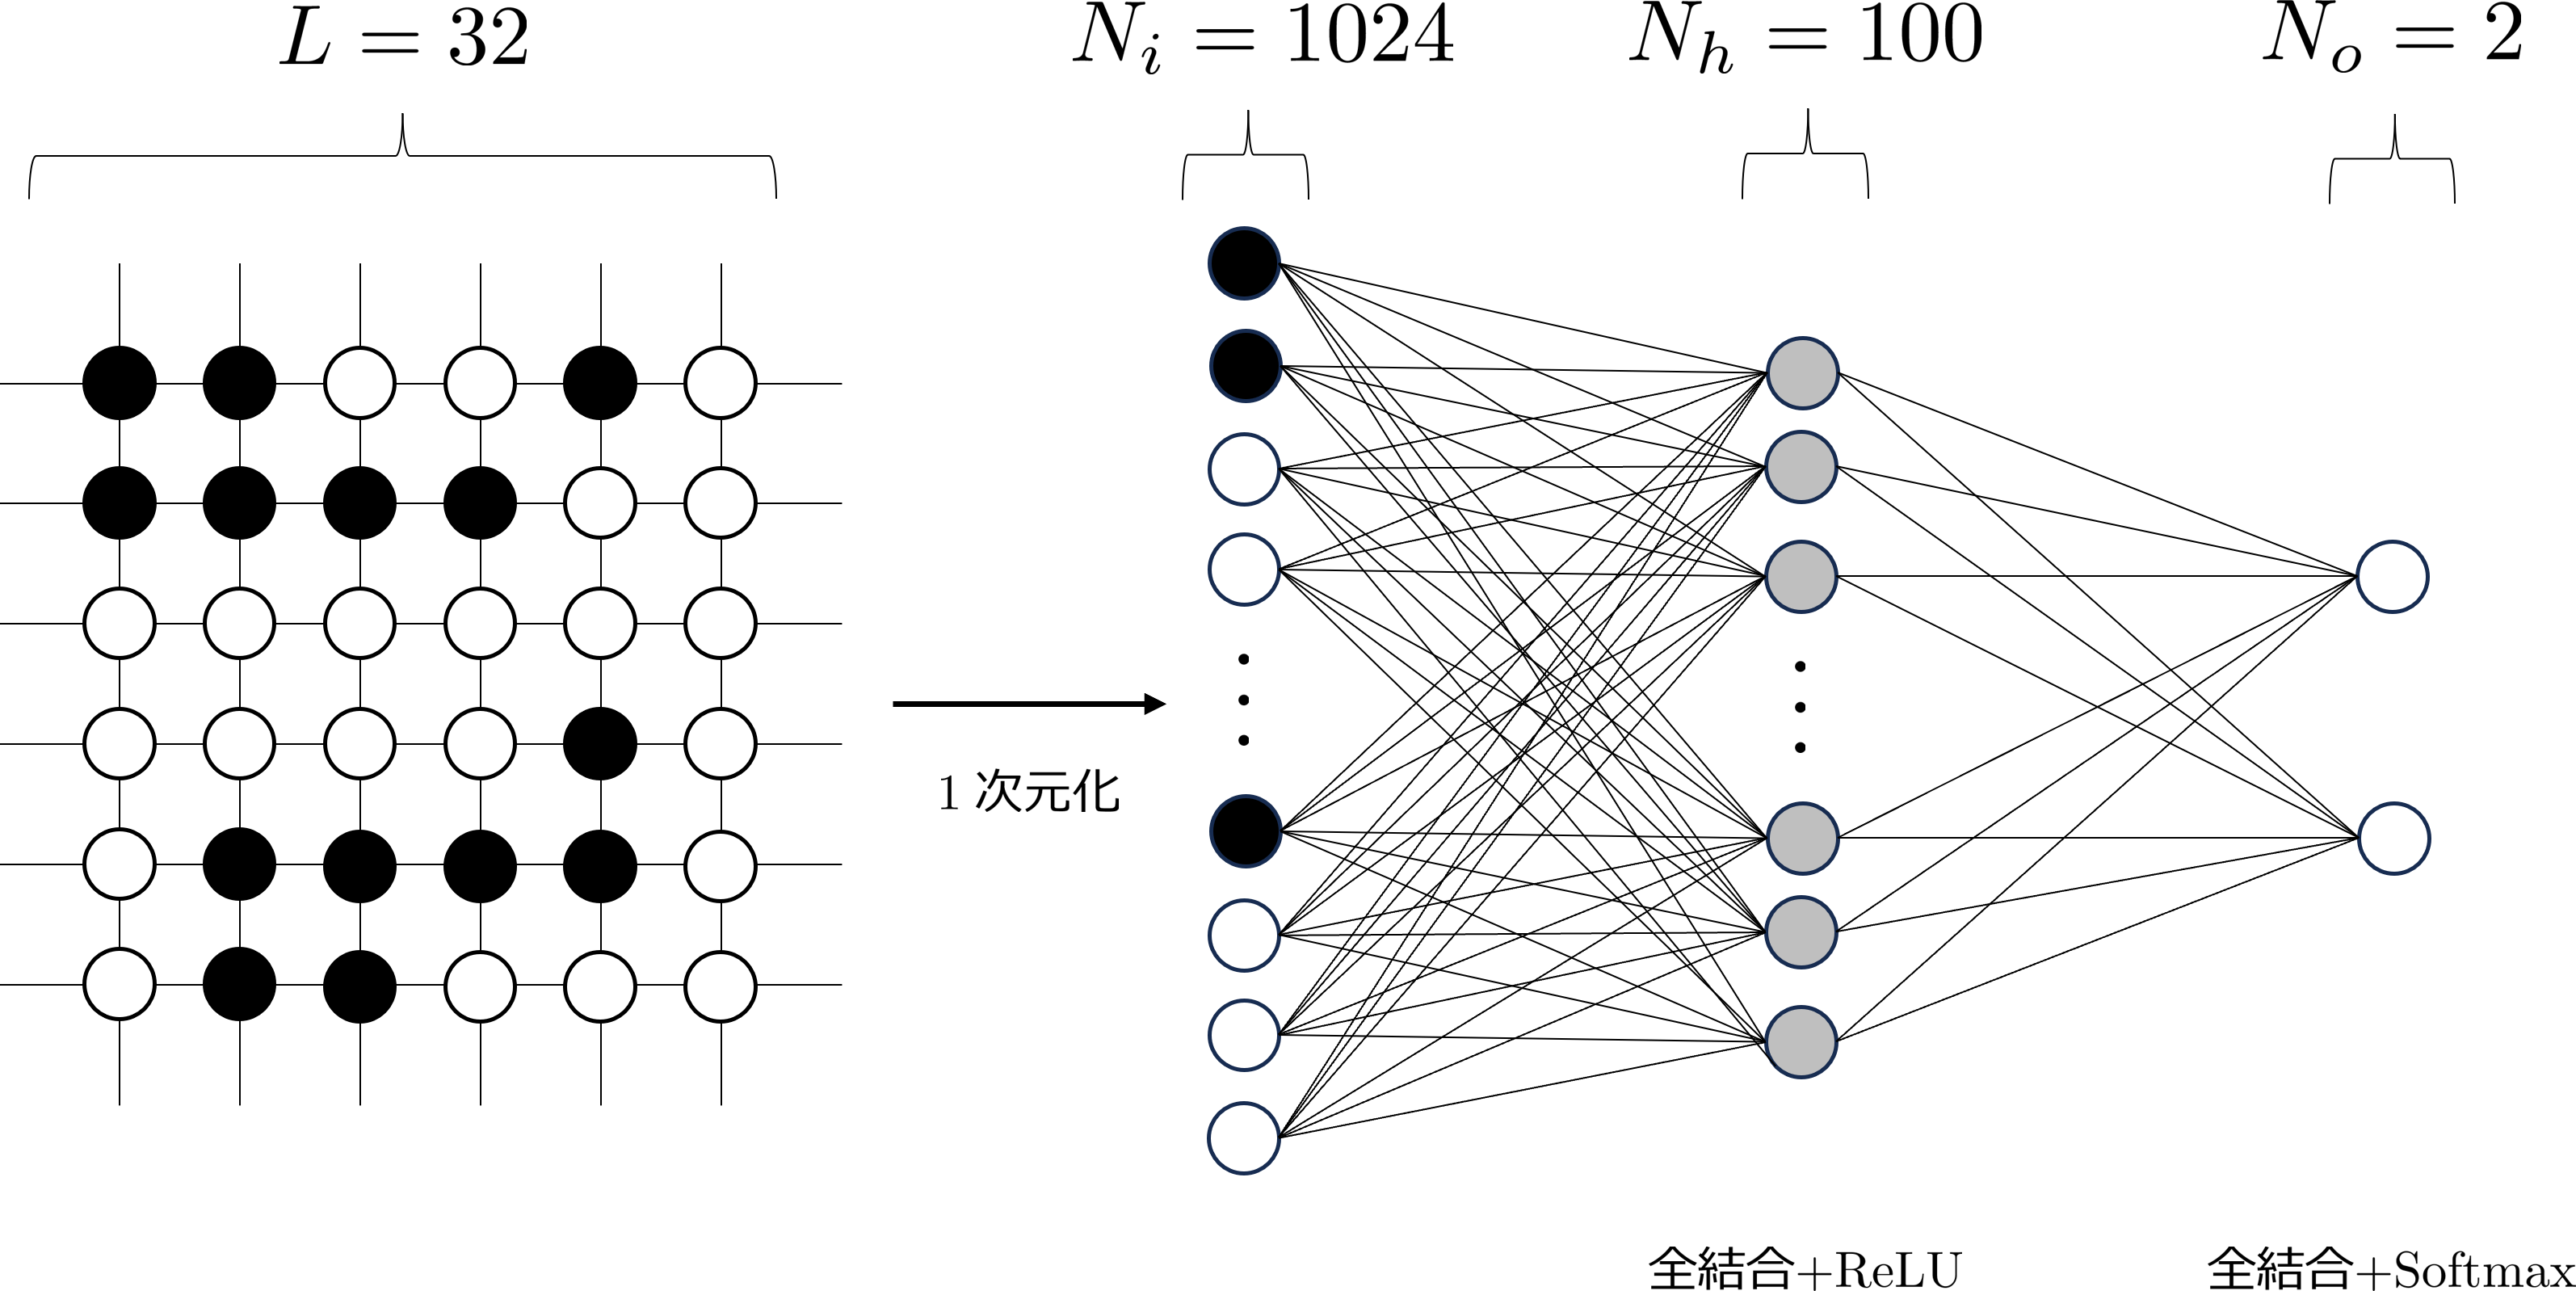
\includegraphics[height=7cm]{image/相分類FCNモデル.png}
    \caption{FCNモデル}
    \label{相分類FCNモデル}
  \end{center}
\end{figure}

2次元のスピン配位は適切な方法で一次元化を行ったあとにニューラルネットワークの入力層のユニットに入力させる.このニューラルネットワークは隠れ層が1層のシンプルな全結合ニューラルネットワークを採用した.
入力層は入力データが入力されるため,ユニットの数はスピン配位の数と等しい値にしなければならない.今回$32 \times 32 = 1024$個のスピン変数が入力されるため,1024個のユニットで設定した.次に隠れ層のユニット数であるが,これは任意に選ぶことができる.今回はユニット数100で設定した.また,隠れ層のユニットには活性化関数としてReLU関数を用いた.したがって,隠れ層での出力$z_i$は
\begin{equation}
  z_i 
  = \mathrm{max}\{0,u_i\}, \quad
  u_i^{(1)} = \sum_{j=1}^{1024} W_{ij}^{(1)} \sigma_j + b_i^{(1)}
\end{equation}
となる.最後に出力層のユニット数だが,今回,強磁性相か常磁性相かを判定する二値分類タスクであるため.ユニット数は2で設定する必要がある.また,0から1の確率で出力させるために.活性化関数はシグモイド関数を用いた.したがって最終的なモデルの出力は
\begin{equation}
  \hat{y}_i 
  = \frac{e^{u_i}}{1 + e^{u_i}}, \quad
  u_i^{(2)} = \sum_{j=1}^{100} w_{ij}^{(2)} z_j + b_i^{(2)}
\end{equation}
となる.

次に,CNNモデルについて説明する.次のような順伝播を行うモデルを構築した.
\begin{equation}
  \begin{bmatrix}
    \begin{aligned}
       & \mathcal{I} = \left\{ \{ \sigma_i \} \Big| \ \text{Ising configs on} \ L \times L \ \text{lattice.} \right\} \\
       & \downarrow
      \begin{cases}
        \text{Convolutional Layer}_{[N_f^2\text{-filter}, \ (s,s)\text{-stride}]} \\
        \text{ReLU activation} \\
        \text{Flatten}
      \end{cases} \\
       & z_i^{(1)} \in \mathbb{R}^{N_h^{(1)} = L^2/s^2} \ \text{: hidden units} \\
       & \downarrow
      \begin{cases}
        \text{Fully-connected layer} \\
        \text{ReLU activation}
      \end{cases} \\
       & z_i^{(2)} \in \mathbb{R}^{N_h^{(2)}} \ \text{: hidden units} \\
       & \downarrow
      \begin{cases}
        \text{Fully-connected layer} \\
        \text{Softmax activation}
      \end{cases} \\
       & y_K \in [0,1]^{2} \ \text{: output units}
    \end{aligned}
  \end{bmatrix}
\end{equation}
また,図$\ref{相分類CNNモデル}$はCNNモデル概要図である.

\begin{figure}[H]
   \begin{center}
       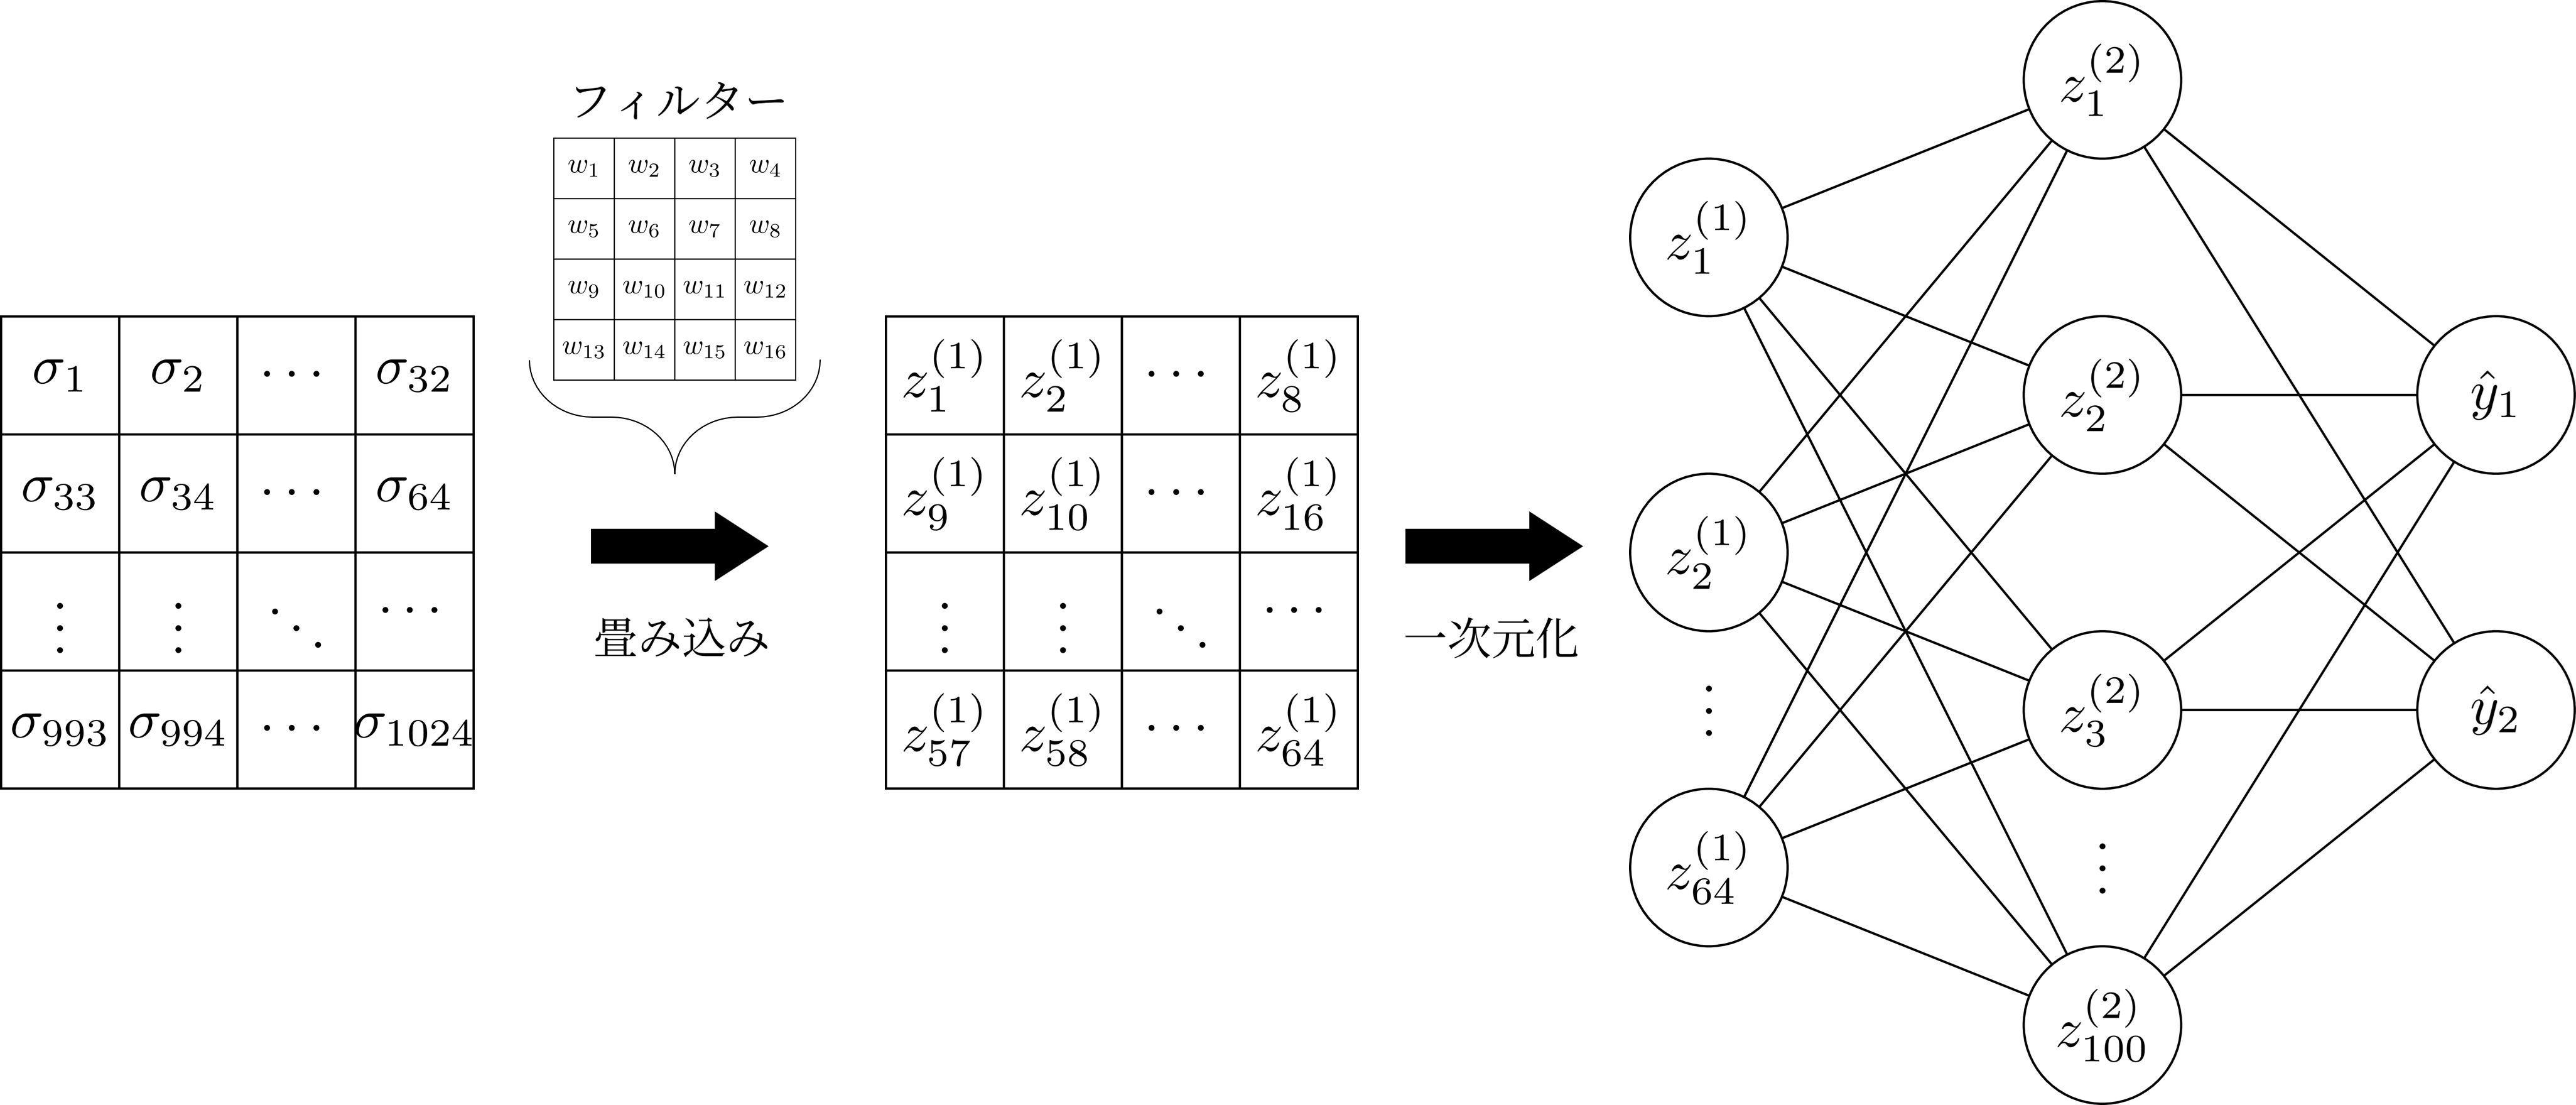
\includegraphics[width=\linewidth]{image/相分類CNNモデル.png}
       \caption{CNNモデル}
       \label{相分類CNNモデル}
   \end{center}
\end{figure}

FCNモデルとの違いは,一次元化を行う前にフィルタによる畳み込みを行っているということである.今回は$32 \times 32$のスピン配位に対して,$4 \times 4$のフィルターで畳み込みを行った.フィルターの数は1つにし,ストライドは$(4,4)$にした.また,パディングは行っていない.そのため,畳み込みを行った後,配位のサイズは$8 \times 8$に縮小する.各変数の値は次のようになる.
\begin{equation}
  z_{(i,j)}^{(1)}
  = \sum_{p,q=0}^{3} w_{p,q}^{(1)} \sigma_{4i+p,4j+q}^{(1)}
\end{equation}
ただし,畳み込み層ではバイアスを入れていない.畳み込みにより,配位のサイズが$8 \times 8$に縮小された後に,一次元化を行う.したがって,全結合部分の最初の層のユニット数は$8 \times 8 = 64$に設定する必要がある.それ以降の層はFCNモデルと全く同じに設定した.\par
この2種類のモデルを作成した1800個のデータセットを使って学習させる.今回,1800個あるデータを各ラベル45個ずつの900個のデータセット2つに分割し,片方を学習データ,もう片方をテストデータとして用いた.\par
学習データによるモデルを学習では,精度を向上させるためにいくつか工夫を行った.以下の表は実際の学習で用いたものである.

\begin{table}[]
  \centering
  \begin{tabular}{cc} \hline
    バッチサイズ & 32 \rule[0pt]{0pt}{1pt} \\ \hline
    エポック数 & 10(FCNモデル),\quad 20(CNNモデル) \rule[0pt]{0pt}{1pt} \\ \hline
    誤差関数 & 交差エントロピー誤差 \rule[0pt]{0pt}{1pt} \\\hline
    最適化アルゴリズム & Adam \rule[0pt]{0pt}{1pt} \\\hline
    学習率 & 0,001 \rule[0pt]{0pt}{1pt} \\\hline
  \end{tabular}
  \caption{学習の設定値}
  \label{学習で用いたもの}
\end{table}

今回,バッチサイズ32のミニバッチ学習で学習を行った.エポック数とは全学習データを何周学習させるかを表すパラメータである.この値は,学習の収束具合をみて設定する必要がある.今回はFCNモデルには10,CNNモデルには20で設定した.また,誤差関数は2値分類のタスクに最適な交差エントロピー誤差を採用し,最適化アルゴリズムにはAdamを使用し,学習率はどちらのモデルも0.001で設定した.\par
この設定で2種類のモデルを誤差逆伝播法よりパラメータ最適化を行った.学習を行っただけでは,過学習が起きている可能性があるため,テストデータで精度を確認しながら学習を行った.次の図\ref{正方イジングFCNloss},図\ref{正方イジングCNNloss}はそれぞれ,エポックごとの損失関数と精度の値を訓練データとテストデータに対してプロットしたグラフである.グラフを見てわかる通り,エポックが増えるごとに訓練データとテストデータどちらも損失関数の値が小さくなり,精度も上がっていることが見て取れる.これは,学習がうまく進んでいることを表している.

\begin{figure}[H]
  \begin{center}
    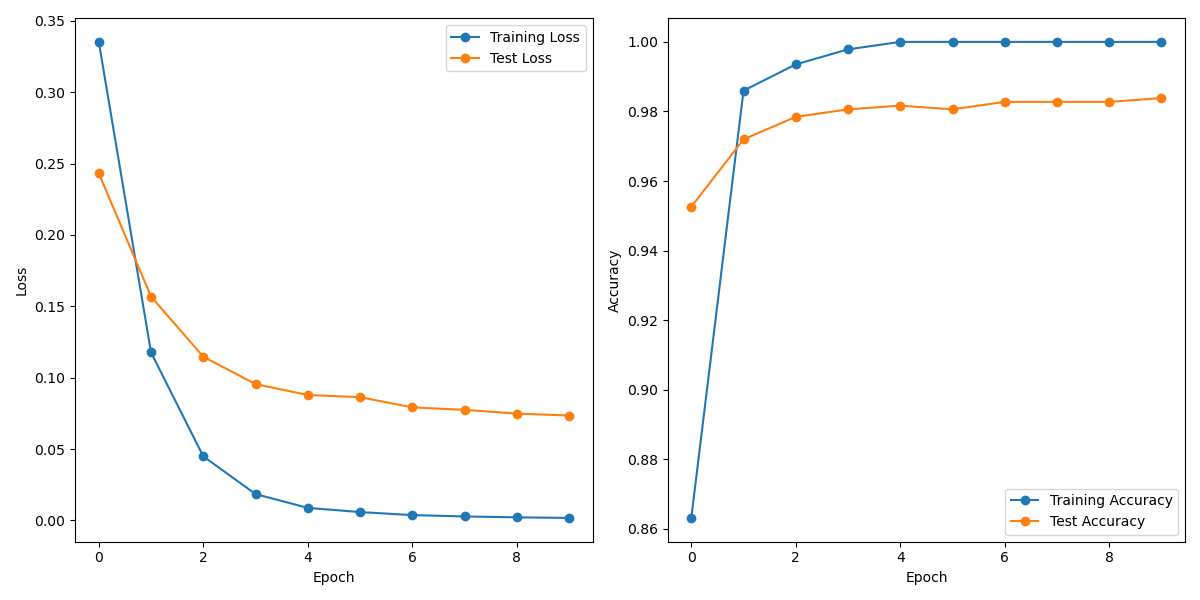
\includegraphics[width=\linewidth]{image/plot_square_FCNN_2.png}
    \caption{FCNモデルによる正方イジング模型のスピン配位の学習結果.横軸はエポック数である.縦軸は左の図は損失関数,右の図は精度である.}
    \label{正方イジングFCNloss}
  \end{center}
\end{figure}
\begin{figure}[H]
  \begin{center}
    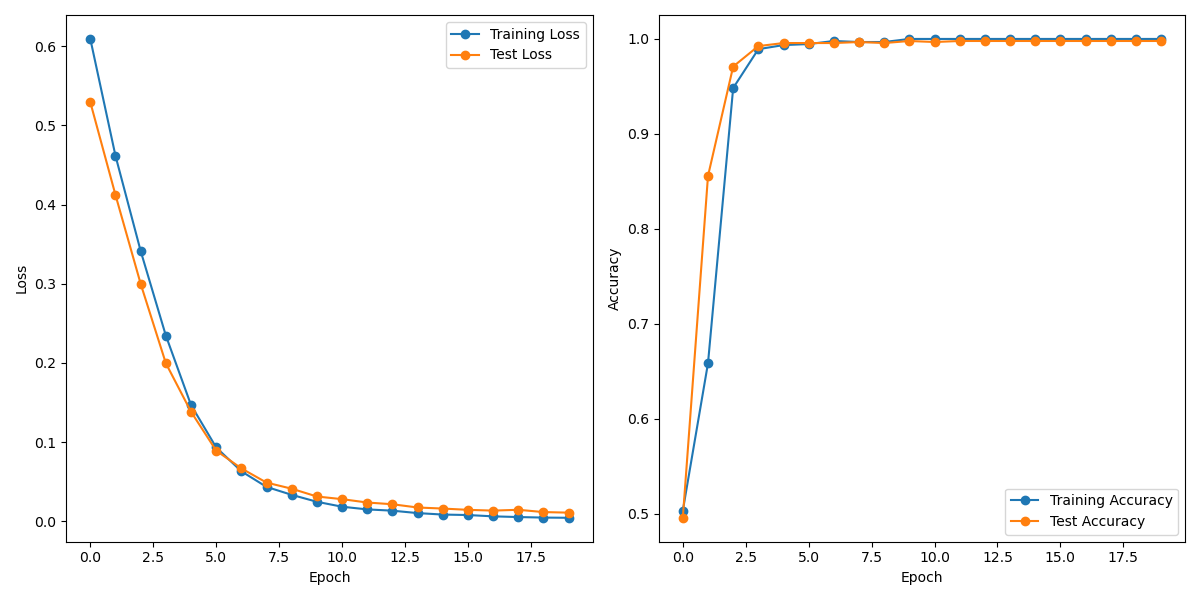
\includegraphics[width=\linewidth]{image/plot_square_CNN_2.png}
    \caption{CNNモデルによる正方イジング模型のスピン配位の学習結果.横軸はエポック数である.縦軸は左の図は損失関数,右の図は精度である.}
    \label{正方イジングCNNloss}
  \end{center}
\end{figure}

テストデータを用いて,各逆温度ラベルでモデルがどのような値を出力したか図\ref{相分類器FCN結果},図\ref{相分類器CNN結果}に示した.各ラベルでの値は,各レベルに対してすべてのテストデータ45に対する出力の平均を出力している.
\begin{figure}[H]
  \begin{minipage}[b]{0.45\linewidth}
    \begin{center}
      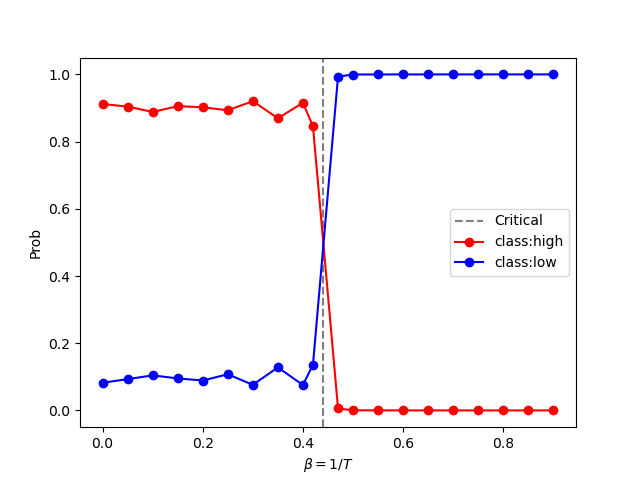
\includegraphics[keepaspectratio, scale=0.4]{image/plot_square_FCNN.png}
      \subcaption{FCN}
      \label{相分類器FCN結果}
    \end{center}
  \end{minipage}
  \begin{minipage}[b]{0.45\linewidth}
    \begin{center}
      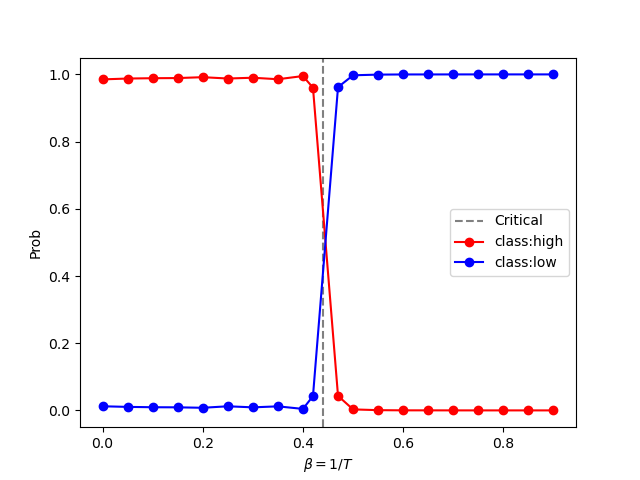
\includegraphics[keepaspectratio, scale=0.4]{image/plot_square_CNN.png}
      \subcaption{CNN}
      \label{相分類器CNN結果}
    \end{center}
  \end{minipage}
  \caption{各温度ラベルにおける出力値の平均をプロットした図.左の図はFCNモデルの結果,右の図はCNNモデルの結果である.また,赤のプロットは常磁性相である確率,青のプロットは強磁性相である確率にである.}
\end{figure}
図からわかるように,どちらのモデルの強磁性相か常磁性相かを正しく分類できていることがわかる.また,この実験では強磁性相はどちらのモデルも精度がほぼ100\%となり,常磁性相ではFCNモデルでは約90\%,CNNモデルではほぼ100\%という結果になった.画像に特化している畳み込み演算を加えたモデルのほうが精度が高いのは納得がいく.


% \subsection{三角イジング模型の相の分類}
% 正方イジング模型の相分類器のモデルをそのまま三角イジング模型から作成した教師ありデータで相の分類を行えるかの実験を行った.結果は以下のようになった.





\section{温度測定器による相転移自動検出}
相の分類器の実験でニューラルネットワークが2次元イジング模型のスピン配位に対して強磁性相か常磁性相を分類できることがわかった.しかし,この相の分類器の実験では,モデルに相転移の情報を与える必要があった.つまり,事前に系の相転移温度がわかっている場合でしか,この検出器は作れないということである.これでは,使える場面が限られてしまうので,どうにかしてモデルに相転移温度の情報を与えないで相の検出を行えるようにしたい.\par
2017年に富谷昭夫と田中章詞によって,ニューラルネットワークでスピン配位の温度を測定するモデルを学習することでイジング模型の相転移を検出することができることがわかった.この実験では,相転移を直接分類するのではなく,まずスピン配位からその配位の温度を予測するモデルを作成し,その学習されたモデルの重みパラメータの値から相転移点を予測することができるというものである.以下では,温度測定器による相転移の検出について説明する.

\subsection{学習データ}
今回の実験ではニューラルネットワークを用いて温度を測定するモデル構築するため,スピン配位と温度ラベルのデータセットを用いる.これは相の分類器のデータセット作成のときよりも簡単である.今回もメトロポリス法を用いて以下のような手順でデータを生成した.\par
\begin{enumerate}
  \item 逆温度ラベル$\beta_i, \ i=1,2,\dots,N_{\text{label}}$を設定する.
  \item 以下を$i=1,2,\dots,N_{\text{label}}$まで繰り返す.
  \begin{enumerate}
    \item メトロポリス法を用いて逆温度$\beta_i$のスピン配位$\bm{\sigma}$を$N$個サンプルする
    \item $(\bm{\sigma},\beta_i)$とする.
  \end{enumerate}
\end{enumerate}
今回,$8 \times 8, 16 \times 16$でそれぞれデータセットを作成した.すべて温度ラベル$\beta_i$は0.2から1までを100等分した値を使用し,各逆温度ラベルに対して,100個のスピン配位を生成した.つまり,それぞれ全データ数は10000になる.

\subsection{モデルの構築と学習}
データセットの生成について説明したので,次にモデルの構築とその学習手順について説明する.まず,今回も相の分類器のときと同様に全結合層のみからなるモデル(FCNモデル)と畳み込み層を加えたモデル(CNNモデル)の2種類のモデルで学習を行った.\par
各モデルについて詳細を説明する.まずFCNモデルは次のような順伝播を行うモデルを使用した.
\begin{equation}
  \left[
    \begin{aligned}
      & \mathcal{I} = \left\{ \{ \sigma_i \} \Big| \ \text{Ising configs on} \ L \times L \ \text{lattice.} \right\} \\
       & \downarrow
      \begin{cases}
        \text{Flatten} \\
        \text{Fully-connected layer} \\
        \text{ReLU activation}
      \end{cases} \\
       & x_a \in \mathbb{R}^{N_h} \ \text{: hidden units} \\
       & \downarrow
      \begin{cases}
        \text{Fully-connected layer} \\
        \text{Softmax activation}
      \end{cases} \\
       & y_K \in [0,1]^{N_o=100} \ \text{: output units}
    \end{aligned}
    \right]
\end{equation}
図\ref{温度測定器FCNモデル}はこの順伝播について図で表したものである.
\begin{figure}[H]
  \begin{center}
    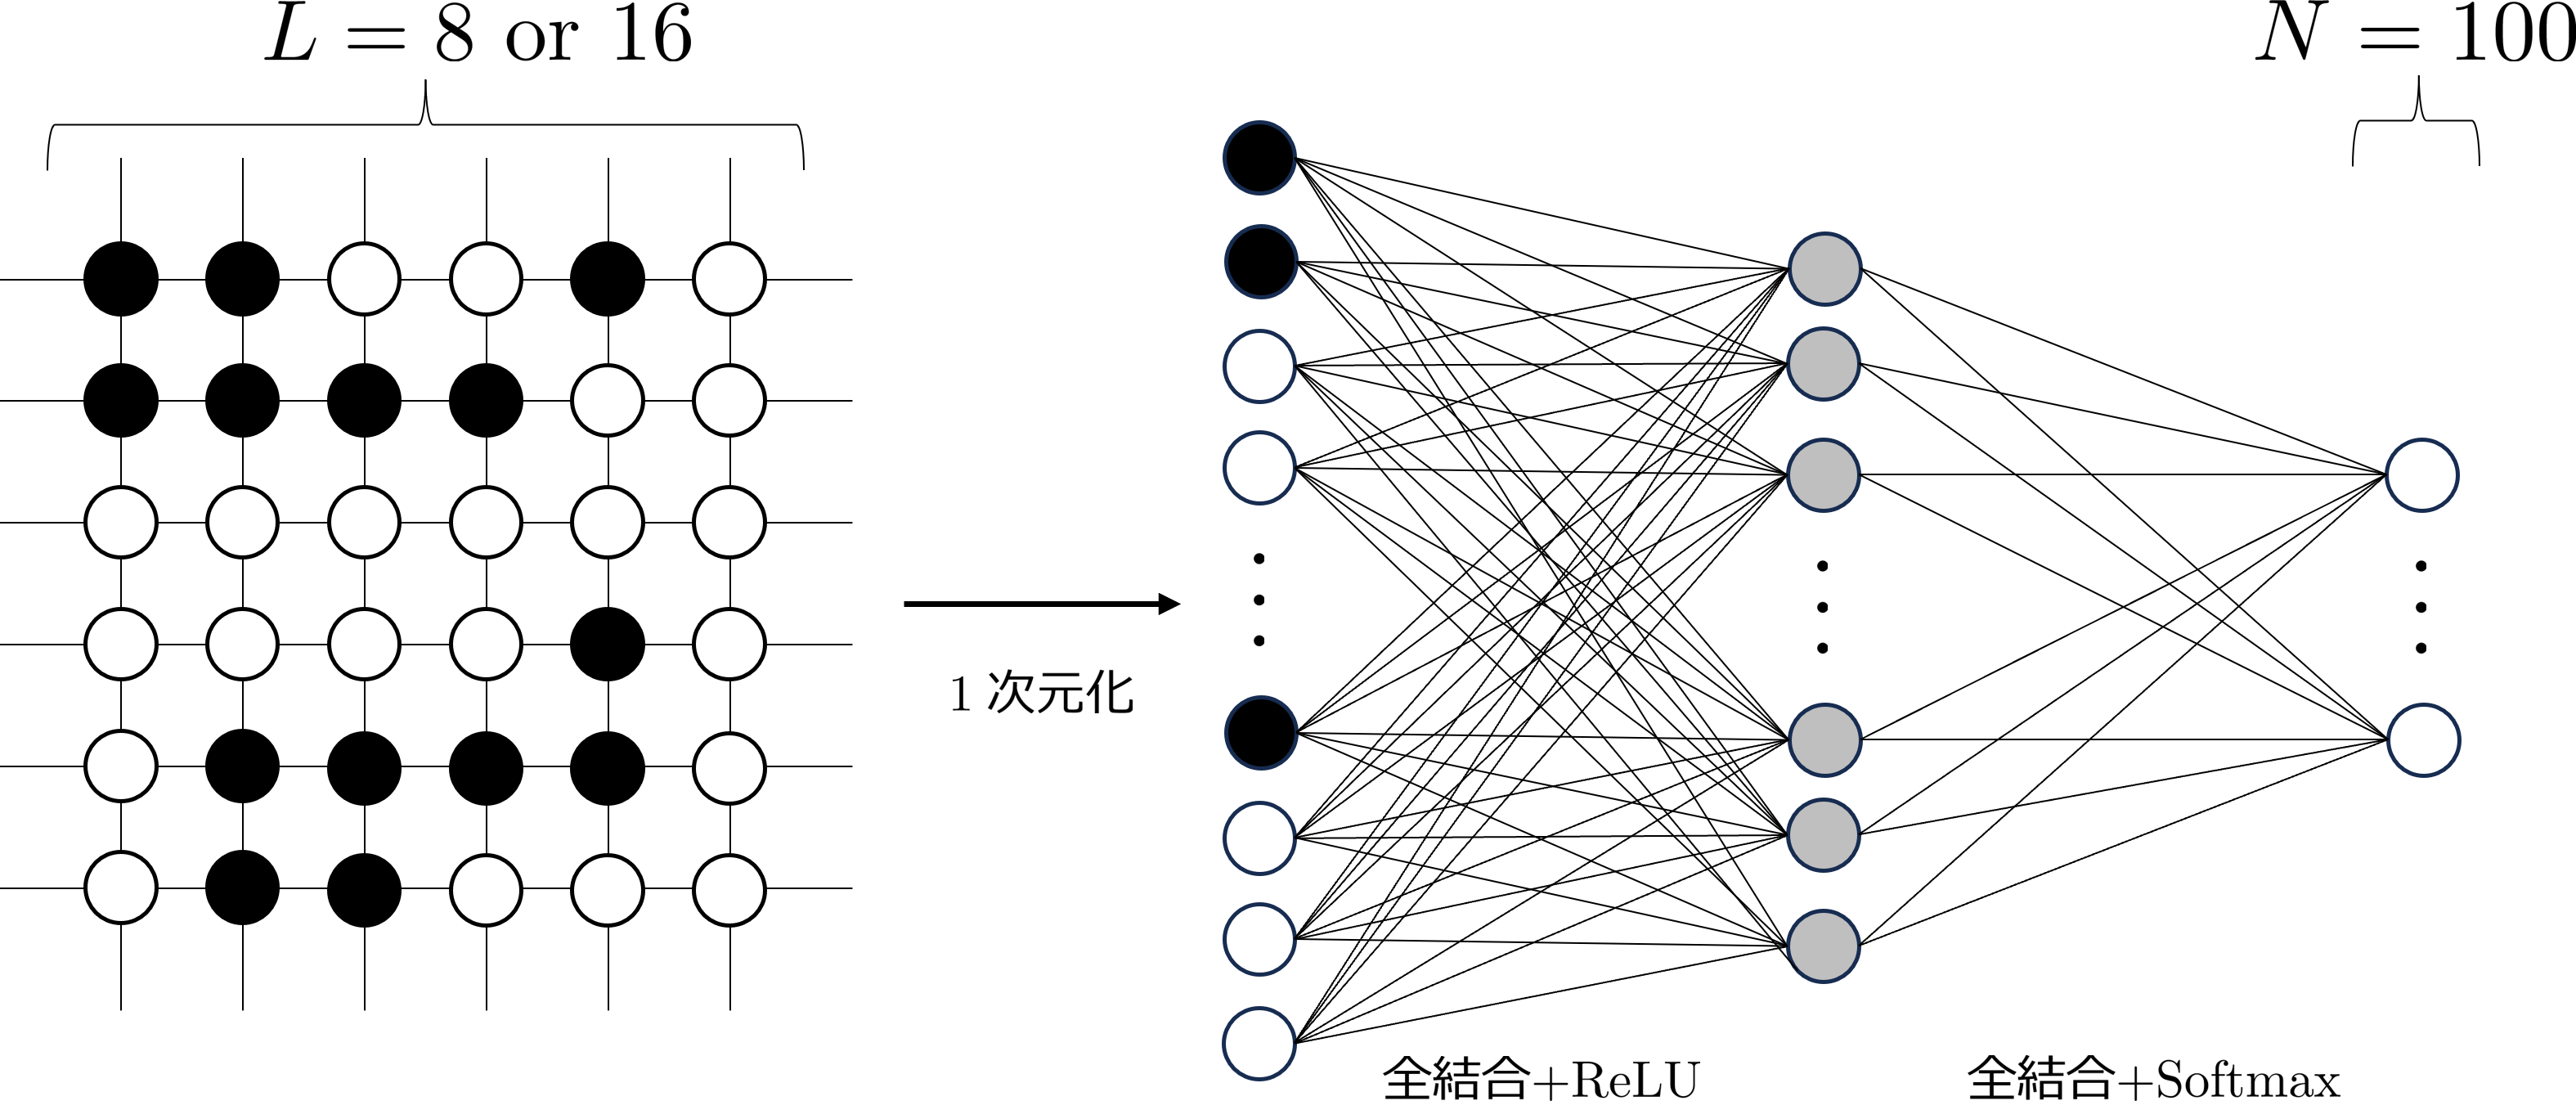
\includegraphics[height=5cm]{image/温度測定器FCN.png}
    \caption{FCNモデル}
    \label{温度測定器FCNモデル}
  \end{center}
\end{figure}
これは中間層が1層のシンプルな全結合ニューラルネットワークである.活性化関数は中間層でReLU関数,出力層では確率で出力するためにSoftmax関数を使用した.今回中間層のユニットの個数は$L=8$のとき$N_h=80$,$L=16$のとき$N_h=320$で学習を行った.\par
次にCNNモデルについて説明する.CNNモデルでは次のような順伝播を行うモデルを使用した.
\begin{equation}
  \begin{bmatrix}
    \begin{aligned}
       & \mathcal{I} = \left\{ \{ \sigma_i \} \Big| \ \text{Ising configs on} \ L \times L \ \text{lattice.} \right\} \\
       & \downarrow
      \begin{cases}
        \text{Convolutional Layer}_{[N_f^2\text{-filter}, \ (s,s)\text{-stride}, \ C_1\text{-channels}]} \\
        \text{ReLU activation} \\
        \hspace{2cm} \vdots \\
        \text{Convolutional Layer}_{[N_f^2\text{-filter}, \ (s,s)\text{-stride}, \ C_i\text{-channels}]} \\
        \text{ReLU activation} \\
        \text{Flatten}
      \end{cases} \\
       & x_a \in \mathbb{R}^{N_h = L^2/s^2 \times C_i} \ \text{: hidden units} \\
       & \downarrow
      \begin{cases}
        \text{Fully-connected layer} \\
        \text{Softmax activation}
      \end{cases} \\
       & y_K \in [0,1]^{N_o} \ \text{: output units}
    \end{aligned}
  \end{bmatrix}
\end{equation}
図\ref{温度測定器CNNモデル}はこの順伝播について図で表したものである.
\begin{figure}[H]
  \begin{center}
    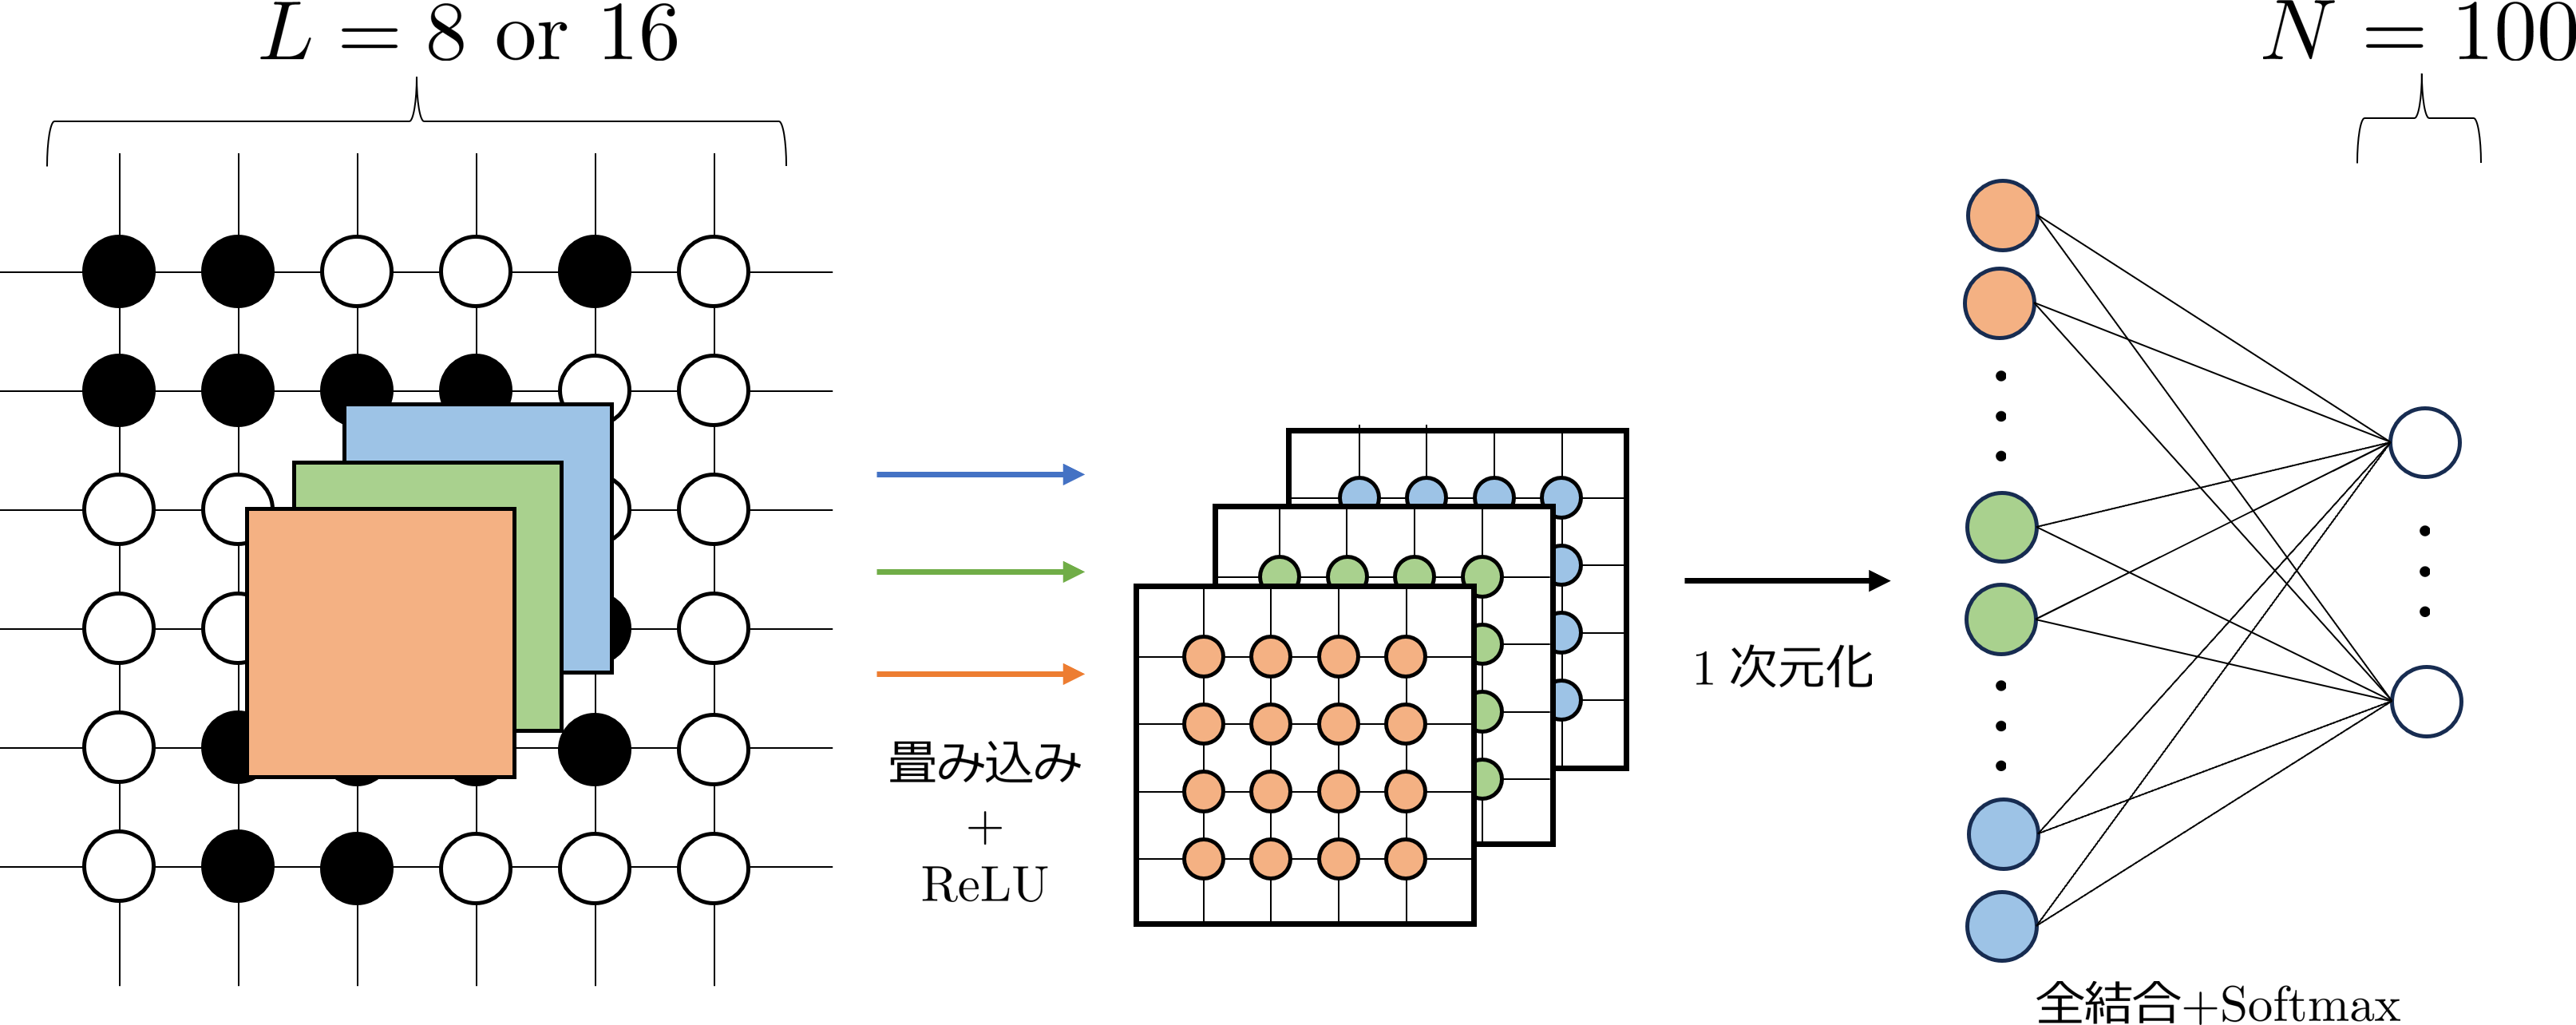
\includegraphics[height=5cm]{image/温度測定器CNN.png}
    \caption{CNNモデル}
    \label{温度測定器CNNモデル}
  \end{center}
\end{figure}
見てわかる通り,畳み込み層と全結合層からなる.こちらもシンプルなモデルを使用している.畳み込み層ではハイパーパラメータとして,カーネルサイズ,ストライド,パッディングサイズ,フィルタのチャンネル数を設定する必要がある.今回,$L=8$と$L=16$のときで以下のように値を設定した.
\begin{center}
  \begin{tabular}{|l|c|c|} \hline
    ハイパーパラメータ& $8 \times 8$ & $16 \times 16$ \\ \hline
    カーネルサイズ & 3 & 5 \\
    ストライド & 2 & 2 \\ 
    パディングサイズ & 1 & 2 \\ 
    チャンネル数 & 5 & 5 \\ \hline 
  \end{tabular}
\end{center}
このような値に設定することで,中間層のユニットの個数を$L=8$のときは80,$L=16$のときは320となり,FCNと同じ個数にすることができる.これにより,モデルの比較がしやすくなる.\par
これら2つのモデルを学習を行った.今回も相分類器の実験のときと同様な方法で10000あるデータを5000個の学習データと5000個のテストデータに分けて学習を行った.以下,学習で用いたパラメータや手法を表でまとめた.
\begin{table}[H]
  \centering
  \begin{tabular}{cc} \hline
    バッチサイズ & 1 \rule[0pt]{0pt}{1pt} \\ \hline
    エポック数 & 1 \rule[0pt]{0pt}{1pt} \\ \hline
    誤差関数 & 交差エントロピー誤差 \rule[0pt]{0pt}{1pt} \\\hline
    最適化アルゴリズム & Adam \rule[0pt]{0pt}{1pt} \\\hline
    学習率 & 0.0001 \rule[0pt]{0pt}{1pt} \\\hline
  \end{tabular}
  \caption{hoge}
  \label{学習で用いたもの2}
\end{table}


\begin{figure}[H]
  \begin{minipage}[b]{0.45\linewidth}
    \begin{center}
      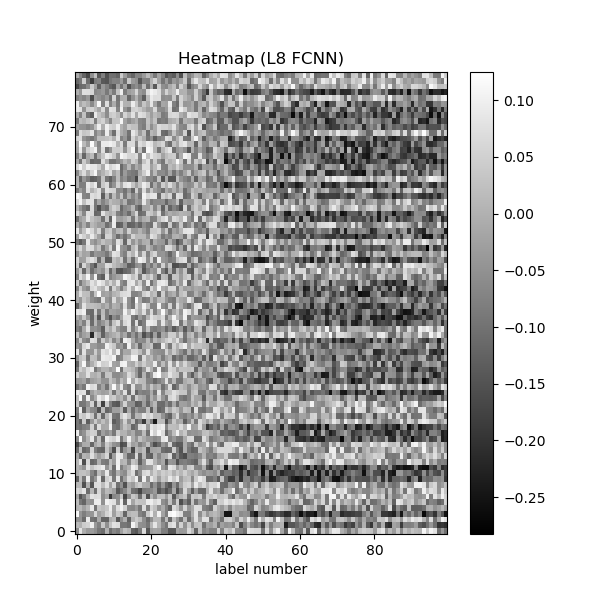
\includegraphics[keepaspectratio, scale=0.45]{image/L8_FCNN_weight.png}
      \subcaption{L8_FCN}
    \end{center}
  \end{minipage}
  \begin{minipage}[b]{0.45\linewidth}
    \begin{center}
      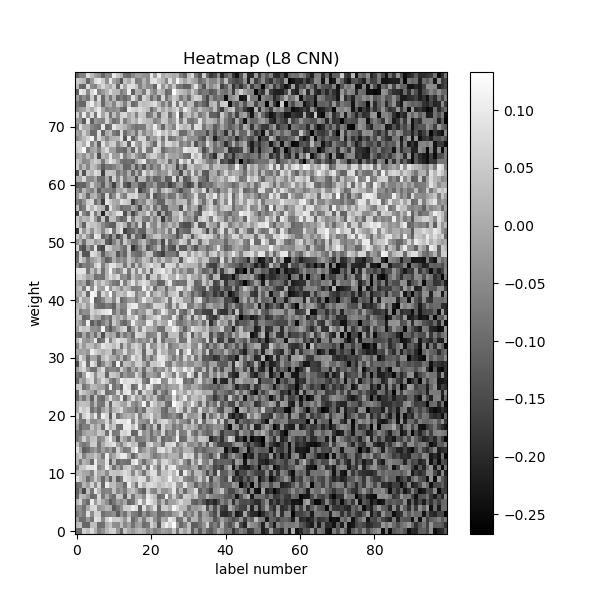
\includegraphics[keepaspectratio, scale=0.45]{image/L8_CNN_weight.png}
      \subcaption{L8_CNN}
    \end{center}
  \end{minipage}
\end{figure}


\begin{figure}[H]
  \begin{center}
    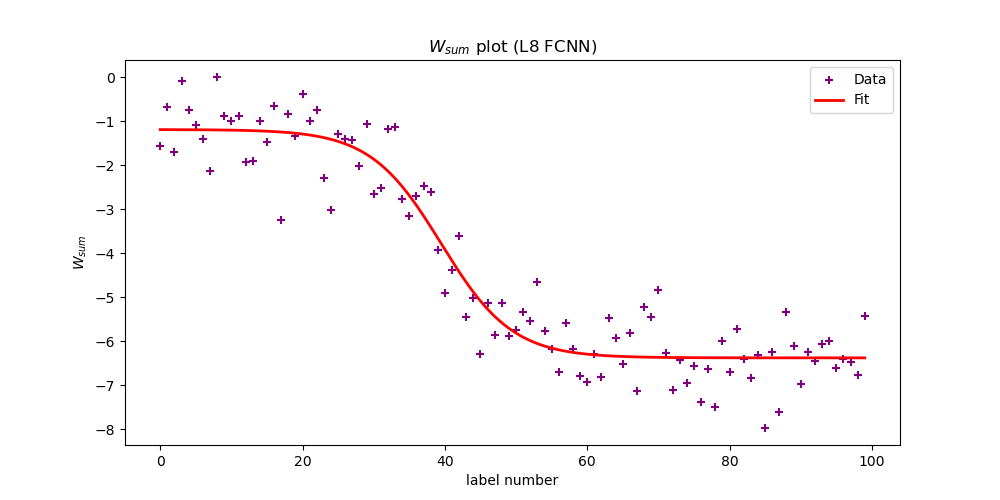
\includegraphics[width=\linewidth]{image/L8_FCNN_weight_sum.png}
    \subcaption{aaa}
    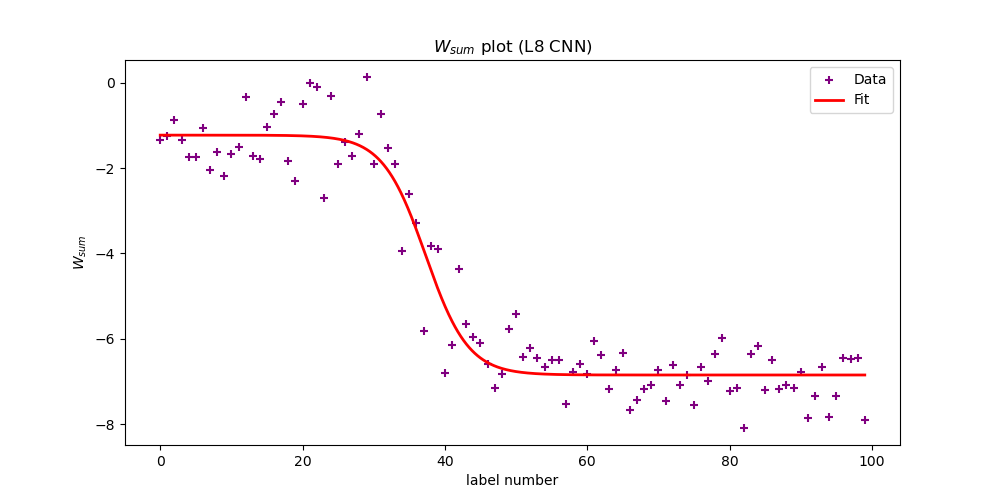
\includegraphics[width=\linewidth]{image/L8_CNN_weight_sum.png}
    \subcaption{bbb}
  \end{center}
  \caption{ccc}
\end{figure}

\begin{figure}[H]
  \begin{minipage}[b]{0.45\linewidth}
    \begin{center}
      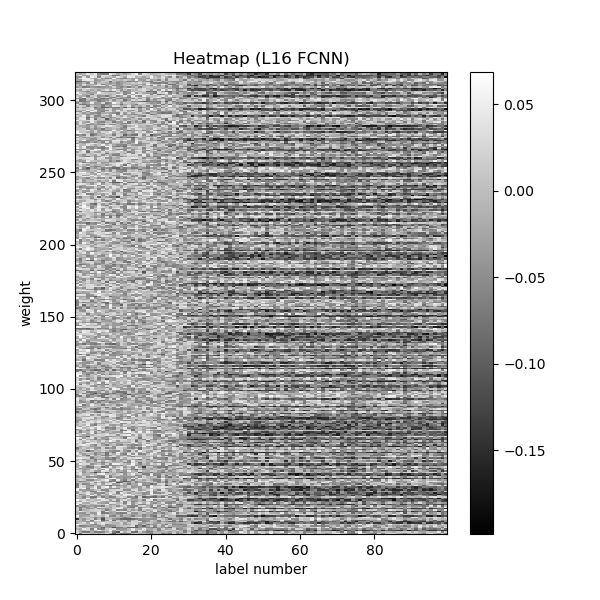
\includegraphics[keepaspectratio, scale=0.5]{image/L16_FCNN_weight.png}
      \subcaption{L16 FCN}
    \end{center}
  \end{minipage}
  \begin{minipage}[b]{0.45\linewidth}
    \begin{center}
      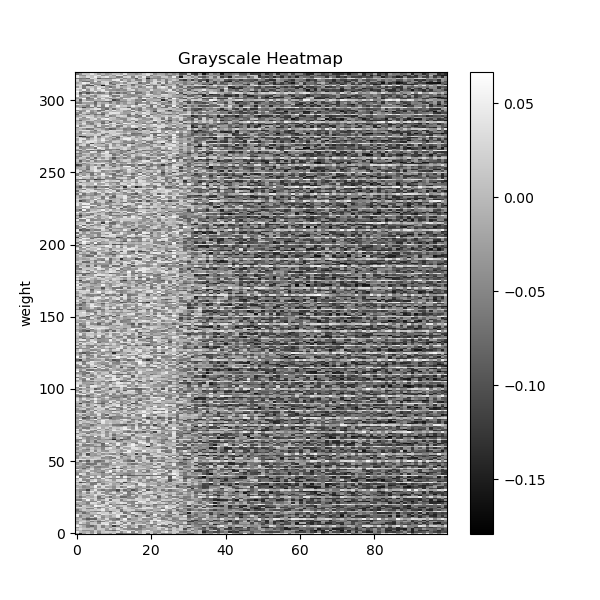
\includegraphics[keepaspectratio, scale=0.5]{image/L16_CNN_weight_2.png}
      \subcaption{L16 CNN}
    \end{center}
  \end{minipage}
\end{figure}

\begin{figure}[H]
  \begin{center}
    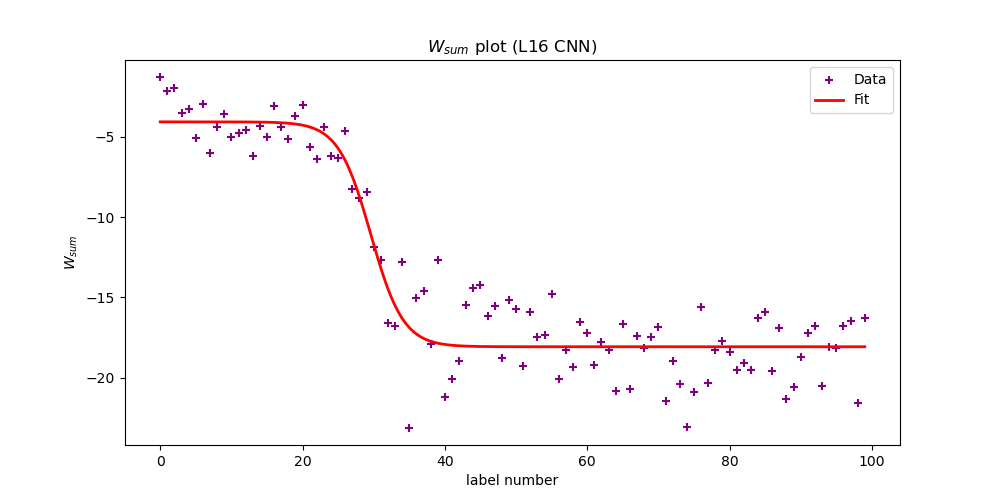
\includegraphics[width=\linewidth]{image/L16_FCNN_weight_sum.png}
    \subcaption{aaa}
    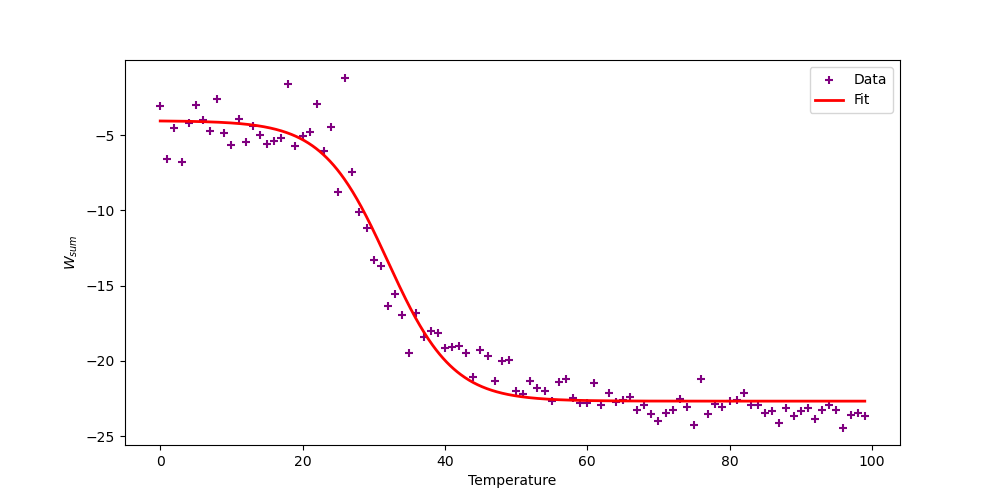
\includegraphics[width=\linewidth]{image/L16_CNN_weight_sum_2.png}
    \subcaption{bbb}
  \end{center}
  \caption{ccc}
\end{figure}



\section{相転移検出がなぜ可能なのか?}
\subsection{臨界温度予測}
2次元イジング模型を考える.ハミルトニアンは
\begin{equation*}
  H(\bm{\sigma}) = - J \sum_{\langle i,j \rangle} \sigma_i \sigma_j
\end{equation*}
ここで,$J$は結合定数,$\sigma_i \in \{ -1, 1 \}$は,サイズが$L \times L$の正方格子のサイトに存在するスピンの自由度(スピン変数)で,周期的境界条件が課されている.和は最近接に対するサイトにわたる.結合定数をボルツマン重みに吸収させて,$e^{-KH}/Z, \ \ K = \beta J$とすることで,ハミルトニアンを次のように再定義する.
\begin{equation}
  H(\bm{\sigma}) = - \sum_{\langle i,j \rangle} \sigma_i \sigma_j
\end{equation}
ここで,$Z = \sum_{\bm{\sigma}}e^{-KH(\bm{\sigma})}$は分配関数である.\par
私たちは,その2次相転移に関連する臨界温度を検出しようと試みている.しかしながら,最初は,教師あり順伝播ニューラルネットワークを用いて温度測定器を構築することを行う.その後,学習されたニューラルネットワークの重みとバイアスを調べ,2次元イジング模型と3状態のポッツ模型の臨界温度を特定しようと試みる.\par
メトロポリス・ヘイスティングス法を用いて,各温度で2000個のイジングスピン配位を生成する.これらは,20の目標温度と一緒にニューラルネットワークに供給される.私たちは,TENSORFLOWをバックエンドに使用したKERASパッケージを用いて,全結合ニューラルネットワークと畳み込みニューラルネットワークの2種類のアーキテクチャを実装した.\par
全結合ニューラルネットワーク:
\begin{equation}
  \left[
    \begin{aligned}
       & \mathcal{I} = \left\{ \{ \sigma_i \} \Big| \ \text{Ising configs on} \ L \times L \ \text{lattice.} \right\} \\
       & \downarrow
      \begin{cases}
        \text{Fully-connected (Dense) layer} \\
        \text{Softmax activation}
      \end{cases}                                                                            \\
       & x_a \in [0,1]^{N_h} \ \text{: hidden units}                                                                  \\
       & \downarrow
      \begin{cases}
        \text{Fully-connected (Dense) layer} \\
        \text{Softmax activation}
      \end{cases}                                                                            \\
       & y_K \in [0,1]^{N_o} \ \text{: output}
    \end{aligned}
    \right]
\end{equation}

入力の自由度は$\{ \sigma_i \} \ (i=1,2,\dots,L \times L)$で,イジングモデルの場合スピンに対応する.隠れ層のユニット$x_a \ (a=1,2,\dots,N_b)$は
\begin{equation}
  x_a = \text{softmax}(w_{ai}^{(1)}\sigma_i + b_a^{(1)})
  \equiv \frac{e^{w_{ai}^{(1)}\sigma_i + b_a^{(1)}}}{\sum_a e^{w_{ai}^{(1)}\sigma_i + b_a^{(1)}}}
\end{equation}
ここで,アインシュタインの縮約記法を使用していることに注意.2つ目の層は,重み$w_{\alpha a}^{(2)}$とバイアス$b_{\alpha}^{(2)}$に置き換えたものである.最終層の変数$y_K \ (K=1,2,\dots,N_o)$は隠れ層と同じ形をとる
\begin{equation}
  y_k = \text{softmax}(w_{ai}^{(2)}\sigma_i + b_a^{(2)})
\end{equation}
出力$\{ y_K \}$に基づいて,入力配位の温度は
\begin{equation}
  K^{\text{output}} = \underset{K} {\operatorname{argmax}} (y_K)
\end{equation}
で決定される.つまり,温度$\alpha$は確率分布$y_K$の中から最も値が高い成分が採用されるということである.学習は,Adamという最適化手法を用いて,交差エントロピー
\begin{equation}
  E(y_K,\bm{1}_{K=K_i^{\text{target}}}) = - \frac{1}{N_o}\sum_i \bm{1}_{K=K_i^{\text{target}}} \ln{y_k}
\end{equation}
という誤差関数を最小することによって実装した.ここで,$i$ は入力配位のラベルを示す.インジケーター関数は次のように定義される.\par
\begin{equation}
  \bm{1}_{K=K_i^{\text{target}}} =
  \begin{cases}
    1 & (K=K_i^{\text{target}}) \\
    0 & (\text{otherwize})
  \end{cases}
\end{equation}

畳み込みニューラルネットワークは3つの畳み込み層と最後の全結合層からなる構成をしており,式(\ref{conv model})である.これについての詳細はセクション3.2で説明する.\par
配位生成から相転移検出までの手順を以下に示す.
\begin{enumerate}
  \item マルコフ連鎖モンテカルロ法より,配位を生成:
  \item ニューラルネットワークを温度計として学習する.入力はスピン配位,出力は予測温度.
  \item ニューラルネットワークに現れる学習済みの重みとバイアスを分析する.マシンパラメーターに相転移の情報がどのように含まれるかについて説明する.
\end{enumerate}

\subsection{2次元イジング模型}
% \begin{figure}[hb]
%   \begin{center}
%     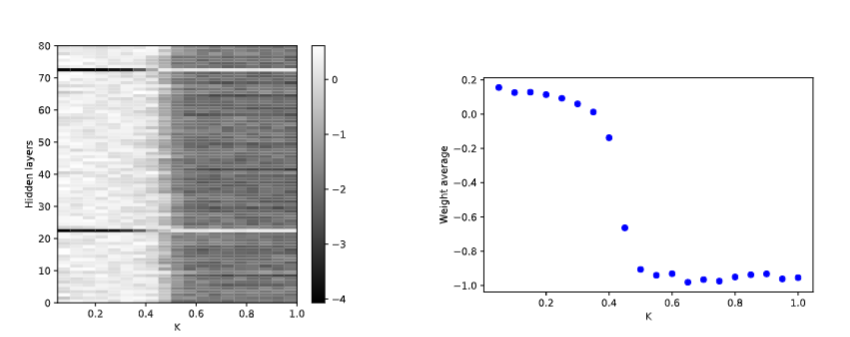
\includegraphics[height=5cm]{image/Figure1.png}
%     \caption{2次元イジング模型における学習後の全結合層での重みの値とそれらを平均した値.横軸はそれぞれ入力配位の温度$K$を表している.縦軸は左の図はニューラルネットワークの隠れ層につながるエッジにおける重みの値に対応し,右の図はその重みの値を$K$での平均をとったものである.重みの平均の値は,厳密な臨界温度$K_{\text{c}}^{\text{exact}}\simeq 0.4407$付近で大きく変化していることが見て取れる.}
%   \end{center}
% \end{figure}
最初に,[4] (田中さんと富谷さんの論文)で既に研究されている2D Ising模型を見ていく.このモデルは,100の目標温度で調査され,その重みは秩序変数のように振る舞い,すなわち自発的な磁化を示す.私たちの主な目的は臨界温度を定量的に推定することではなく,そのメカニズムを理解することなので,目標温度の数を20に減少させる.具体的には,$K = 0.05, 0.1, 0.15, \dots, 1.0$のような値である.ニューラルネットワークより教師あり機械学習を行った.

図1の2D Ising模型の場合,全結合層の重みおよびそれらの学習後の平均について説明する.横軸は入力配位の温度Kを表し,左のパネルの縦軸はニューラルネットワークの隠れユニットに接続された成分に対応している.右のパネルの縦軸は,各Kに対する重みの平均を示している.重みの平均値は,正確な臨界温度$K_e^{\text{exact}} \approx 0.4407$の周りで著しく変化している.


格子サイズは$L = 16$であり,隠れユニットの数は$N_h = 80$,そして$N_o = 20$はそれぞれ20の目標温度に対応している.臨界温度は正確に知られており,$K_c^{\text{exact}} = \frac{1}{2}\ln{\sqrt{2}+1} \approx 0.4407$である.学習後の2層目の重みが図1である([4]より).臨界温度は重みの和を$c_1 \tanh{[c_2(K-K_c)]}$でフィッティングしてパラメータ$c_1,c_2,c_3$を導くことで予想する.実験では格子サイズ$L=8,16,32$で行った.実際,最終的な重みの平均は秩序変数のように振る舞うようです(図1の右パネル).次のセクションで重みの詳細な構造について議論する.

\subsection{ニューラルネットワークでエンコードされた磁化}
% \begin{figure}[H]
%   \begin{center}
%     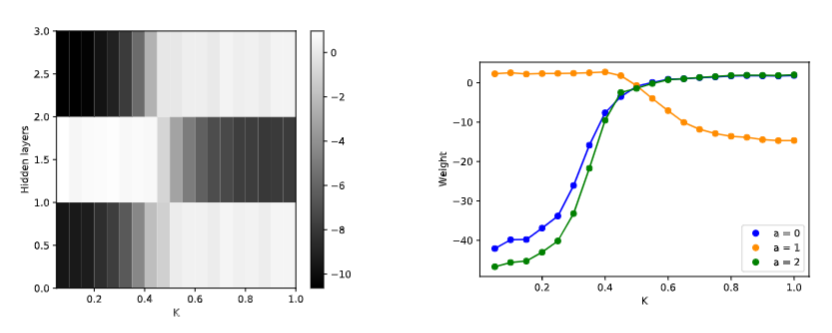
\includegraphics[height=5cm]{image/Figure3.png}
%     \caption{隠れ層のユニットが3つ$(N_h=3)$の学習済みニューラルネットワークにおける全結合層の重み$w_{Ka}^{(2)}$の値.横軸は2次元イジング模型での温度$K$を表している.臨界温度付近で構造に変化が起きていることがわかる.真ん中の重みだけ値が反対になっている.}
%   \end{center}
% \end{figure}
% \begin{figure}[hb]
%   \begin{center}
%     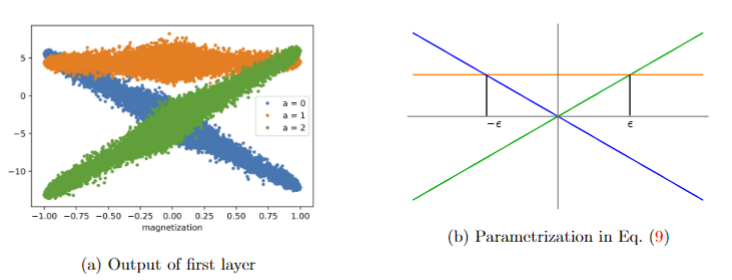
\includegraphics[height=5cm]{image/Figure4.png}
%     \caption{(a)第1層目の出力と入力配位の磁化の相関.横軸は入力配位の各サイトでの磁化,縦軸は$\tilde{x}_a=w_{ai}^{(1)}\sigma_i+b_a^{(1)}$である.(b)フィッティングしたもの.}
%   \end{center}
% \end{figure}
相転移の秩序変数が2D Ising模型において自発磁化であることから,学習後にはその情報がニューラルネットワークにエンコードされていることは自然なことと言える.定量的な論拠を示すために,2D Ising模型の場合において学習されたニューラルネットワークの重みとバイアスを調査して,簡略化されたモデルを構築する.最初に、簡略化のために(2)の中の隠れユニットの数を80から3に減少させる.図3に示されているように,それでも臨界温度を捉えていることに気づく.\par
第二層をモデリングする前に,まず最初の層の特性を調査する.図4は,式(3)の第一層の出力$\tilde{x}_a \equiv w_{ai}^{(1)}\sigma_i + b_a^{(1)}$と,入力のIsingスピン配位の磁化密度との相関を示している.この観察から,私たちはこれらの出力から,図4bに示すように,磁化$m(\{ \sigma \})$に対して線形な三つのラインでモデリングする.
\begin{equation}
  \tilde{x} =
  \begin{pmatrix}
    \tilde{x}_0 \\ \tilde{x}_1 \\ \tilde{x}_2
  \end{pmatrix}
  =
  \begin{pmatrix}
    -m \\ \epsilon \\ m
  \end{pmatrix}
\end{equation}
ここで,$\epsilon > 0$は定数である.さらに,活性化関数として,私たちの目的のためにsoftmaxの代わりに最大値を1,それ以外を0にする最大値関数を使用している.この変更は最終結果に影響を与えない.$x_a = \max{(\tilde{x}_a)}$は次のベクトルを生成する.
\begin{equation}
  m<-\epsilon : x=
  \begin{pmatrix}
    1 \\ 0 \\ 0
  \end{pmatrix}, \
  -\epsilon \leq m < \epsilon : x=
  \begin{pmatrix}
    0 \\ 1 \\ 0
  \end{pmatrix}, \
  \epsilon \leq m : x=
  \begin{pmatrix}
    0 \\ 0 \\ 1
  \end{pmatrix},
\end{equation}
パラメータ$\epsilon$は、強磁性相と常磁性相を分離する閾値磁化と解釈できる[3].\par
三つの隠れユニットの磁化依存性を理解したら,次に第二層を分析する.この層の重みは図3に示されている.温度を低温,臨界温度,高温の三つの部分に分割する.それぞれ以下のベクトルで表される.
\begin{equation}
  \text{Low} \ \text{K} :
  \begin{pmatrix}
    1 \\ 0 \\ 0
  \end{pmatrix}, \
  \text{Critical} \ \text{K} :
  \begin{pmatrix}
    0 \\ 1 \\ 0
  \end{pmatrix}, \
  \text{High} \ \text{K} :
  \begin{pmatrix}
    0 \\ 0 \\ 1
  \end{pmatrix},
\end{equation}
No-dimensional output spaceにおいて.この手法により,出力次元$N_o$を実質的に3に削減する.図3に従って,私たちは以下のように重みをパラメータ化する.
\begin{equation}
  w^{(2)} =
  \begin{pmatrix}
    -\Delta & 0       & -\Delta \\
    -\delta & -\delta & -\delta \\
    0       & -\Delta & 0
  \end{pmatrix}
\end{equation}
ここで,$\Delta > \delta > 0$.行列$w^{(2)}$の$Ka$成分は$w_{Ka}^{(2)}$に対応する.バイアスは重みよりもはるかに小さいため,無視する.厳密なパラメータ化は,以下の議論には必要ない.このとき,$y_K = \max{(\tilde{y}_K)}=\max{(w_{Ka}^{(2)}x_a+b_K^{(2)})}$は以下の出力を生む.
\begin{align}
  m<-\epsilon : y_K = \max(w_{K0}^{(2)}) =
  \begin{pmatrix}
    0 \\ 0 \\ 1
  \end{pmatrix}, \\
  -\epsilon \leq m < \epsilon : y_K = \max(w_{K1}^{(2)}) =
  \begin{pmatrix}
    1 \\ 0 \\ 0
  \end{pmatrix}, \\
  \epsilon \leq m : y_K = \max(w_{K2}^{(2)}) =
  \begin{pmatrix}
    0 \\ 0 \\ 1
  \end{pmatrix},
\end{align}
これらはそれぞれ,低温,高温,低温と予想される.$m<-\epsilon$と$m>\epsilon$のスピン配位は秩序相にあるため,正しく予想できている.また,$-\epsilon \leq m < \epsilon$もまた,正しく予想されている.ただし,この場合には中間温度,つまり臨界温度を検出することができない.さらに,式(\ref{}) に三つ以上の対象温度を導入しても,学習されたニューラルネットワークは順序/無秩序相内の異なる温度を区別することができない.なぜなら,図3で示されているように,重み(およびバイアス)の上部ブランチはそれぞれ$K_c$より上と下でほぼ温度に依存しないからである.したがって,高温または低温のみを区別することができる.\par
これは,三つの隠れユニットにより単一の閾値パラメータ$\epsilon$しか持たないことが原因かもれない.隠れユニットをさらに導入することで閾値パラメータの数を増やすことができる.しかし,これは温度の高い精度にはつながらない.実際,隠れユニットの数を増やしても、,二層の重みは温度依存性の二つのパターンしか示さない.つまり,多くは図3の青と緑の曲線のようにふるまい,残りはオレンジの振舞いを見せる.これは,図1で観察されている現象とまさに一致している.隠れユニットを増やすことは単に,すでに図3で観察された第二層の重みを複製する結果となり,その結果,導入された隠れユニットの数に関係なく,予測される温度は高いか低いかのどちらかとなる.\par
上記の分析から得られた結論は次の通りである.
ネットワークは,第一層の出力で示す磁化の情報を取得した.しかしながら,ニューラルネットワークは磁化に基づいて秩序相と無秩序相の違いを除いて,温度を区別することは難しい.機械学習パラメータの観点から見ると,これは第二層の重みが臨界温度の周りを除いて温度に依存しないという事実に起因している.

\subsection{エネルギーと温度の予測}
前のサブセクションで,2次元イジング模型の磁化が温度の教師あり全結合ニューラルネットワークに組み込まれていることがわかった.これにより,その重み構造から臨界温度を読み取ることが可能になる.臨界温度はうまく検出されているようだが,温度そのものの予測自体についてはまだ議論していない.興味深いことに,2次元イジング模型の場合,上記の設定で温度学習の精度は理論的に$40.1\%$と計算できる.これは機械学習による温度予測の精度の上限を示しています([32].詳細は付録Aを参照).ただし、全結合ニューラルネットワークによる温度予測のテスト精度は$16.8\%$であり,理論的に予測された$40.1\%$の精度にはほど遠い.これまで,磁化の特徴抽出による相転移の検出を見てきたが,温度測定の観点で学習を行うことでより良い学習ができるのではないか.温度の予測精度が向上するようなニューラルネットワークを構築できた場合,どのようなことが起こるのか?\par
この疑問に答えるために,次に示す畳み込みニューラルネットワークを使用して,より高い精度を実現した.
\begin{equation}
  \begin{bmatrix}
    \begin{aligned}
       & \mathcal{I} = \left\{ \{ \sigma_i \} \Big| \ \text{Ising configs on} \ L \times L \ \text{lattice.} \right\} \\
       & \downarrow
      \begin{cases}
        \text{Convolution}_{[(s_1,s_1)\text{-filter}, \ (s_1,s_1)\text{-stride}, \ C_1\text{-channels}]} \\
        \text{ReLU activation} \\
        \text{Convolution}_{[(s_2,s_2)\text{-filter}, \ (s_2,s_2)\text{-stride}, \ C_2\text{-channels}]} \\
        \text{ReLU activation} \\
        \text{Convolution}_{[(s_3,s_3)\text{-filter}, \ (s_3,s_3)\text{-stride}, \ C_3\text{-channels}]} \\
        \text{ReLU activation} \\
        \text{Flatten}
      \end{cases} \\
       & x_a \in [0,1]^{N_h = L^2/(s_1s_2s_3)^2 \times C_3} \ \text{: hidden units} \\
       & \downarrow
      \begin{cases}
        \text{Fully-connected (Dense) layer} \\
        \text{Softmax activation}
      \end{cases} \\
       & y_{\alpha} \in [0,1]^{N_t} \ \text{: output}
    \end{aligned}
  \end{bmatrix}
\end{equation} \label{conv model}
このネットワークは,3つの畳み込み層から配位されている.それぞれフィルタサイズ$(s_i,s_i)$,ストライド$(s_i,s_i)$,そして,チャンネル数$C_i$であり,それらの間にはReLU関数が入る.その後,出力は全結合層に渡される.この層の入力と出力は私たち興味の対象であり,詳細に分析される.第二最終層の出力,記号で$x_a$と示されるものは,以下のように表される.
\begin{equation}
  x_a = \text{ReLU}(\tilde{x}_a) = \text{Max}(\tilde{x}_a,0)
\end{equation}
これは$[0,\infty)$の範囲の値をとる.$\tilde{x}_a$は前の層のReLU関数の渡す前の出力である.その後、出力$x_a$は全結合層の入力として機能し,式(4)と(5)を通じて温度の予測を行う.\par
前のサブセクションに続き,私たちは,全結合層の入力として機能する3つの隠れユニットを配置し,学習の結果としてニューラルネットワークが何を学習するかを理解しようとする.この目的のために,パラメータは以下のように設定する:
\begin{equation}
  L = 16, \ \ (s_1, s_2, s_3) = (2, 2, 4), \ \ (C_1, C_2, C_3) = (64, 32, 3)
\end{equation}
これにより,隠れ層のユニット数を$N_{\text{h}}=3$にすることができる.このセットアップでは,テストデータセットにたいして$35.9\%$の精度を出すことができた.これは全結合層よりも2倍高いが,統計の不足と非常に少ない隠れユニット数のため,まだ境界に非常に近いわけではない.\par
% \begin{figure}[ht]
%   \begin{center}
%     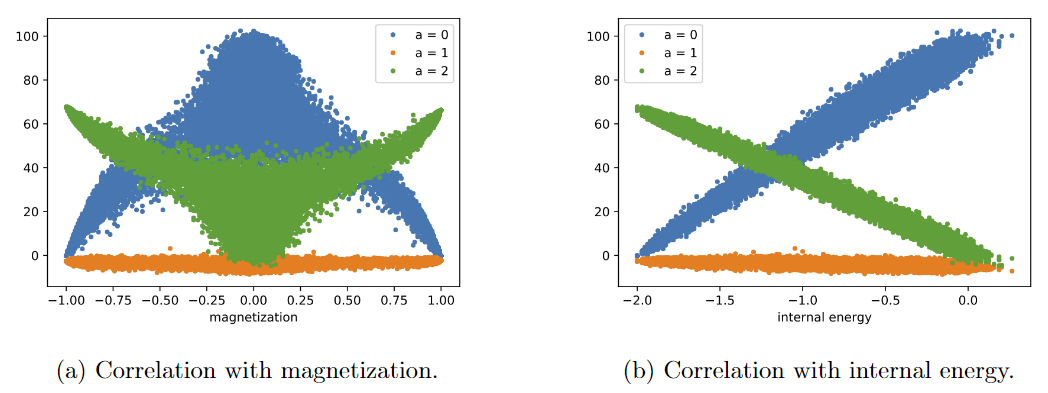
\includegraphics[height=5cm]{image/Figure5.png}
%     \caption{学習されたニューラルネットワークの全結合層の重みと物理量との相関を示すもので,それぞれが左パネルおよび右パネルの垂直軸に対応する5つの隠れユニットがある.(a) および (b) の水平軸は,それぞれ2D Ising 配位の磁化および内部エネルギーを示す.\label{correlation}}
%   \end{center}
% \end{figure}
図\ref{correlation}は,第1層の出力と磁化(図\ref{correlation}a)および内部エネルギー(図\ref{correlation}b)との相関を示している.はっきりとニューラルネットワークが学習した内容の変遷が見て取れる.第1層の出力は,今では入力配位の磁化よりももしろ内部エネルギーに比例している.また,第2層の重みは温度に対して穏やかな依存性を示しており,臨界温度の情報がぼやけていることに気付く(図7);すぐに見るように,振動するオレンジの線は温度の予測には関係ない.\par
次は,最後の2層の簡略なパラメータ設定に進む.ここで,$(w_{ai}^{(1)}, b_a^{(1)})$および$(w_{ai}^{(2)}, b_a^{(2)})$はそれぞれ,最後から2番目の層および最後の層の重みとバイアスを表す.すでに述べたように,および図\ref{correlation}bで確認したように,第1層の出力は入力配位$\{ \sigma_i \}$のエネルギー$E(\{ \sigma_i \})$に比例している.ReLU関数を通ると,
\begin{equation}
  x_a = \text{ReLU}(w_{ai}^{(1)}\sigma_i + b_a^{(1)}), \ \
  x = \begin{pmatrix} x_0 \\ x_1 \\ x_2 \end{pmatrix}
  = \begin{pmatrix} E+2\epsilon \\ 0 \\ -\phi E \end{pmatrix}
\end{equation}
ここで,$\epsilon$と$\phi$は正の定数である.$E$の定義域は、$x_a$が負の値を取らないように制限されている.\par
全結合層の入力が$E$に比例していることを観察したので,入力配位 $\{\sigma_i\}$の温度の最適な推定が何であるかを考えてみよう.配位$\{ \sigma_i \}$が温度$K$で現れる確率$P(\{ \sigma_i \} ; K )$は
\begin{equation}
  P(\{ \sigma_i \} ; K )
  = \frac{e^{-KE(\{ \sigma_i \})}}{Z(K)}
  = e^{-KE(\{ \sigma_i \}) - \ln{Z(K)}}
  = e^{-KE(\{ \sigma_i \}) + F(K)}
\end{equation}
と表せされる.したがって,${\sigma_i}$ が温度$K$で生成される尤度は,
次の「確率」で表される.
\begin{equation}
  y_K^{\text{theory}} = \frac{P(\{\sigma_i ; K \})}{\sum_{K'}P(\{\sigma_i ; K' \})} = \text{softmax}(-KE + F)
\end{equation}
ここで,$F = -\ln{Z(K)}$は自由エネルギーで$K'$はすべてのターゲット温度での足し上げを意味する.このとき,私たちが得る推定温度は
\begin{equation}
  K^{\text{output}} =
  \underset{K} {\operatorname{argmax}} \left[\text{softmax}(-KE + F)\right]
\end{equation}
となる.ここで注記するのは,自由エネルギーが温度$K$の関数であり,有限な系では真の特異性を示さないものの,相転移の情報を保持しているということである.\par
上記の考察に基づいて,私たちのニューラルネットワークの全結合の重みを,その結果の出力が(21)のように振る舞うように推測する.その後,学習されたネットワークの実際のパラメータと比較する,このために,重みを以下のようにパラメータ化する.
\begin{equation}
  w_{K0}^{(2)} = -\phi G(K) - pK + q, \ \
  w_{K2}^{(2)} = -G(K) + rK + s
\end{equation}
定数パラメータ$p,q,r,s$および共通の非線形関数$G(K)$を持つようにする.図7のオレンジの曲線,$w^{(2)}_{K1}$は,$x_1 = \text{ReLU}(\tilde{x}_1) = 0$となるため,私たちの考慮には関係ない.バイアスの値が重みの値よりもはるかに小さい場合,バイアスを無視するというシミュレーションからの観察を利用している.\par
それでは,$y_K = \text{softmax}(w_{Ka}^{(2)}x_a + b_K^{(2)})$で式(19)と(23)を用いると,次のような出力が得られる.
\begin{equation}
  y_K = \text{softmax}(-(p+r)KE - 2\epsilon(\phi G(K) + pK))
\end{equation}
ここで,$\text{max}$関数に影響を与えないため,$K$に依存しない項は落とした.この式は,実際に$-2\epsilon (\phi G(K) + pK) = (p + r)F$が満たされる場合,$y_K^{\text{theory}}$の形をとる.理論的に予測された重みを図6にプロットした.
\begin{equation}
  w_{K0}^{(2)} = \frac{p+r}{2\epsilon}F(K) + q, \ \
  w_{K2}^{(2)} = \frac{p+r}{2\epsilon \phi}F(K) + \left( \frac{p}{\phi} + r \right)K + s
\end{equation}
% \begin{figure}
%   \begin{center}
%     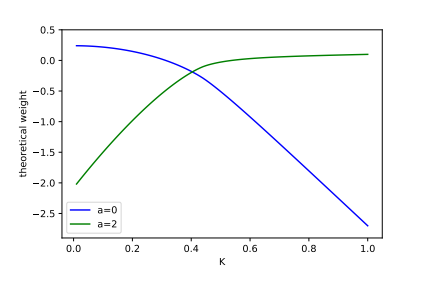
\includegraphics[height=4cm]{image/Figure6.png}
%     \caption{青,緑の線はそれぞれ式(23)の$w_{K0}^{(2)}$と$w_{K2}^{(2)}$を表している.水平軸は,入力の2D Ising配位の温度Kを表している.詳細は本文を参照.}
%   \end{center}
% \end{figure}
% \begin{figure}
%   \begin{center}
%     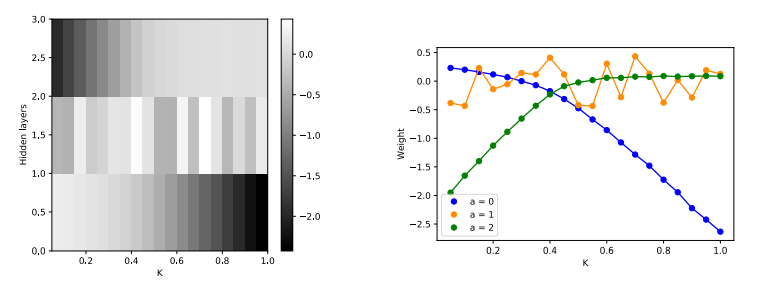
\includegraphics[height=4cm]{image/Figure7.png}
%     \caption{3つの隠れユニット$H_{\text{h}}=3$を持つ学習された畳み込みニューラルネットワークの全結合の重み.水平軸は,入力の2次元Ising模型の温度$K$を表している.最初と最後の重みの値は,以前のケースとは対照的に,温度が上昇するにつれて徐々に変化する.詳細な議論については本文を参照.}
%   \end{center}
% \end{figure}
$F(K)$は2次元Ising模型で解析的に計算された自由エネルギーである.これは,図7に示される学習されたニューラルネットワークから得られた実際の重みと非常によく一致している(青と緑の曲線).これらの考察に基づいて,相転移の情報は再び全結合の重みに符号化されていると結論する.なぜなら,式(23)の$G(K)$は直接的に自由エネルギーと関連しているからである.特に,臨界温度は,温度に関する重みの2階導関数の増加を検出することによって得られる.\par
上記で示したモデルや重みのパラメータ設定は,同じ温度予測を生じる多くの可能性のうちの一つであることに注意してほしい.たとえば.2次の$K$依存性は,重みではなく最後の層のバイアスから生じる可能性がある[32].その場合,相転移や自由エネルギーの情報はバイアスに符号化されるはずである.物理的な情報が機械のパラメータにどのように格納されるかは、隠れユニットの数や活性化関数などを含むニューラルネットワークのアーキテクチャに依存する\par
ニューラルネットワークの内部構造に対する洞察を得たことから,物理的な観点から畳み込みニューラルネットワークが完全に接続された層だけから成るネットワークよりも温度をより正確に予測できる理由について論じる.このセクションで観察したように,後者は中間層で磁化を捉えるが,前者は内部エネルギーを抽出し,それに基づいて温度を推測しようとする.ただし,Ising模型における磁化の温度依存性は,臨界温度周辺以外では内部エネルギーと比較して小さい.したがって,ニューラルネットワークがより正確な温度予測のために内部エネルギーの情報を抽出するのは妥当である.実際,畳み込みニューラルネットワークは内部エネルギーを成功裏に学習して,より高い精度を実現している.畳み込みニューラルネットワークの方が優れたパフォーマンスを発揮する理由は,畳み込み層がIsingスピンの空間的な相関などの空間構造を利用して,入力スピン構造の特徴を識別する能力があるためである.一方で,全結合層はその構造には無視されます.最後に,2次元Ising模型に対して与えられた議論は,3状態ポッツモデルにも当てはまることを触れておく.\par

\section{結論}
私たちは,温度による教師あり機械学習を用いて2次元Ising模型の相転移検出を再検証し,その基本的なメカニズムを明らかにした.\par
まず,全結合ニューラルネットワークが2次元Ising模型および3状態ポッツ模型の学習の結果として,第2層の重み構造に急激な変化を示すことを示した.3つの隠れユニットを持つニューラルネットワークを詳しく調べると,実際には第1層で磁化を捉えていることが明らかになった.相転移の検出は,臨界温度周辺以外の入力配位に対する温度の低い予測精度の結果である.\par
一方で,畳み込みニューラルネットワークを使用することで,温度予測の精度を向上させることに成功した.学習された畳み込みネットワークは,磁化ではなく入力配位の内部エネルギーを捉えていることが判明した.また,最後の全結合層の重みは,前者のケースとは対照的に値に急激な変化を示さず,これは最適な温度予測の観点から理解できます.この場合,重みは自由エネルギーに比例しており,したがって,臨界温度を含む物理的な情報が再びこれに符号化されている.\par
興味深いことに,学習されたニューラルネットワークは,どのように学習されたかによって異なる物理的な情報を抽出する.温度予測の観点から見て「悪い」ニューラルネットワークは,入力スピン構造の磁化を捉えようとしますが,これは臨界温度を検出するのに便利であることがある(これは秩序変数であるため).ネットワークアーキテクチャの改善により,「良い(より良い)」温度予測器を構築することができる.ただし,相転移の情報はネットワークにより暗黙的に符号化される.



% \chapter{機械学習と繰り込み群}
% \section{繰り込み群と特徴抽出}


\chapter*{まとめ}
研究のまとめを書く.

%=====================================================================================
\chapter*{謝辞} %章を付けずにタイトル表示
\addcontentsline{toc}{chapter}{謝辞} %章立てせずに目次に追加するおまじない
この修士論文を完成させるにあたり、多くの方々に支えられ、助言をいただきました。まず初めに、素粒子論研究の阪口教授,百武教授,藤原教授,そして山下助教に心より感謝申し上げます。機械学習ゼミにおいて、多大なるお世話になりました。お陰様で、機械学習やディープラーニングの基礎知識を深めることができ、研究において大きな成果を得ることができました。\par
特に、担当教員である藤原教授には、修論ゼミにおいて大変お世話になりました。緻密なアドバイスや示唆により、論文の進行や内容の向上に大いに貢献いただきました。深い感謝の意を表します。\par
また,同じ研究室の伊藤君には、研究分野が近しいこともあり、数々の相談に乗っていただきました。伊藤君の専門知識と経験から得られたアドバイスは、研究の方向性を明確にする上で非常に有益でした。心から感謝いたします。\par
最後に、私の研究活動において支えてくださったすべての関係者に感謝いたします。皆様のご協力なしでは、この論文の完成はあり得ませんでした。改めて、心より感謝いたします。

%=====================================================================================

% \addcontentsline{toc}{chapter}{参考文献} %章立てせずに目次に追加するおまじない
\renewcommand{\bibname}{参考文献} %これがないと,タイトルが「関連図書」になってしまう
\bibliography{reference} %bibtexファイルの読み込み
\bibliographystyle{junsrt} %本文に\cite{}を入れることで,参考文献表示

% 付録
\appendix
\renewcommand{\thechapter}{\Alph{chapter}}
\renewcommand{\thesection}{\Alph{chapter}.\arabic{section}}
\setcounter{section}{0}
\renewcommand{\theequation}{\Alph{chapter}.\arabic{equation}}
\setcounter{equation}{0}

\chapter{aaa}
aaa
\section{bbb}
bbb


\end{document}